\documentclass[letterpaper, 11pt, openany]{book}
\usepackage{amsthm}
\usepackage[margin=0.75in]{geometry}
\usepackage{enumitem}
\usepackage{fancyhdr}
\usepackage[T1]{fontenc}
\usepackage{newtxtext}
\usepackage[cmintegrals]{newtxmath}
\usepackage{inter}
\usepackage{authoraftertitle}
\usepackage{fontawesome5}
\usepackage{relsize}
\usepackage{xcolor}
\usepackage{bm}
\usepackage{tocloft}
\usepackage{parskip}
\usepackage[hidelinks]{hyperref}
\usepackage{bookmark}
\usepackage{multicol}
\usepackage{cellspace}
\usepackage{mathtools}
\usepackage{graphicx}
\usepackage{titlesec}
\usepackage{comment}

\faStyle{regular}

\vbadness=99999
\pagestyle{fancy}
\renewcommand\headrulewidth{0pt}
\renewcommand\footrulewidth{0pt}

\renewcommand{\chaptermark}[1]{\markboth{\thechapter \ ~ #1}{}}
\renewcommand{\sectionmark}[1]{\markright{\thesection \ ~ #1}}
\renewcommand{\subsectionmark}[1]{}
\renewcommand{\subsubsectionmark}[1]{}

\fancyhf{}
\setlength{\headheight}{18pt}
\setlength{\headsep}{18pt}
\setlength{\footskip}{32pt}

\fancyhead[LE]{\sffamily \textbf{\thepage} \qquad Chapter \leftmark}
\fancyhead[RO]{\sffamily Section \rightmark \qquad \textbf{\thepage}}

%\fancyhead[LO, RE]{\sffamily \textbf{\rightmark}}
%\fancyhead[RO, LE]{\sffamily \textbf{\thepage}}


\fancypagestyle{firstofchapter}{
    \fancyhead{}
    \fancyfoot[RO,LE]{\sffamily \textbf{\thepage}} 
}

\renewcommand \labelenumi{\textbf{\theenumi.}}
\renewcommand \labelenumii{\textbf{\theenumii.}}

\renewcommand \labelitemii{$\circ$}

\newcommand{\scdot}{\boldsymbol{\cdot}}
\newcommand{\redboxed}[1]{{\color{red}\boxed{\color{black}{#1}}}}
\newcommand{\pd}[2]{\frac{\partial #1}{\partial #2}}
\renewcommand{\qedsymbol}{\faSquare}
\newcommand{\curl}[1]{\operatorname{curl}\mathbf{#1}}
\newcommand{\divr}[1]{\operatorname{div}\mathbf{#1}}
\newcommand{\proj}[2]{\operatorname{proj}_{\mathbf{#2}}\mathbf{#1}}
\newcommand{\comp}[2]{\operatorname{comp}_{\mathbf{#2}}\mathbf{#1}}
\renewcommand{\Re}{\operatorname{Re}}
\renewcommand{\Im}{\operatorname{Im}}

\titleclass{\part}{top}
\titleclass{\chapter}{straight}

\titleformat{\part}{\sffamily\huge\fontseries{b}\selectfont}{\thepart}{1em}{}
\titlespacing{\part}{0pt}{18pt plus 0pt minus 18pt}{12pt plus 2pt minus 2pt}

\titleformat{\chapter}{\sffamily\LARGE\fontseries{b}\selectfont}{\thechapter}{1em}{}
\titlespacing{\chapter}{0pt}{18pt plus 0pt minus 18pt}{12pt plus 2pt minus 2pt}

\titleformat{\section}{\sffamily\Large\fontseries{b}\selectfont}{\thesection}{1em}{}
\titlespacing{\section}{0pt}{18pt plus 4pt minus 4pt}{12pt plus 2pt minus 2pt}

\titleformat{\subsection}{\sffamily\large\fontseries{b}\selectfont}{\thesubsection}{1em}{}
\titlespacing{\subsection}{0pt}{18pt plus 4pt minus 4pt}{12pt plus 2pt minus 2pt}

\titleformat{\subsubsection}{\sffamily\fontseries{b}\selectfont}{\thesubsubsection}{1em}{}
\titlespacing{\subsubsection}{0pt}{18pt plus 4pt minus 4pt}{2pt plus 2pt minus 2pt}

\renewcommand{\thefootnote}{\fnsymbol{footnote}}

\renewcommand{\thefigure}{\arabic{chapter}.\arabic{section}.\arabic{figure}}

\renewcommand{\arraystretch}{1.2}

\newtheoremstyle{mytheoremstyle}
    {3pt}{3pt}{\normalfont}{0pt}{\small \sffamily \fontseries{b}\selectfont}{.}{ }{}
\theoremstyle{mytheoremstyle}
\newtheorem{theorem}{Theorem}[section]
\newtheorem{definition}{Definition}[section]

\renewenvironment{proof}{{\par \sffamily \smaller \fontseries{b}\selectfont Proof}}{\hfill\qed}

\newtheoremstyle{myexamplestyle}
    {3pt}{3pt}{\normalfont}{0pt}{\small \sffamily \fontseries{b}\selectfont}{}{5mm}{}
\theoremstyle{myexamplestyle}
\newtheorem{example}{Example}[section]


\newenvironment{solution}{\paragraph{\sffamily \smaller \fontseries{b}\selectfont Solution}}{\hfill\faSquare}
\newenvironment{commentary}{\paragraph{\sffamily \smaller \fontseries{b}\selectfont Comment}}{}
% TODO: change this to a theorem style so it can be referenced and numbered properly
% \newenvironment{definition}{\paragraph{\sffamily \smaller \fontseries{b}\selectfont Definition}}{}

\setcounter{tocdepth}{1}

\setlength{\cftbeforepartskip}{12pt}
\setlength{\cftbeforechapskip}{12pt}
\setlength{\cftbeforesecskip}{0pt}
\setlength{\cftchapnumwidth}{4ex}
\setlength{\cftsecindent}{4ex}
\setlength{\cftsecnumwidth}{7ex}

\renewcommand{\cfttoctitlefont}{\sffamily\large\fontseries{b}\selectfont}
\renewcommand{\cftpartfont}{\sffamily\large\fontseries{b}\selectfont}
\renewcommand{\cftchapfont}{\sffamily\fontseries{b}\selectfont}
\renewcommand{\cftchappagefont}{\sffamily\fontseries{b}\selectfont}
\renewcommand{\cftpartpagefont}{\sffamily\fontseries{b}\selectfont}
\renewcommand{\cftsecfont}{\sffamily\selectfont}
\renewcommand{\cftsecpagefont}{\sffamily\selectfont}
\renewcommand{\cftsubsecfont}{\sffamily\selectfont}
\renewcommand{\cftsubsecpagefont}{\sffamily\selectfont}

\renewcommand{\cftsecdotsep}{\cftnodots}
\renewcommand{\cftsubsecdotsep}{\cftnodots}
\renewcommand{\cftsubsubsecdotsep}{\cftnodots}

%\setlist{leftmargin=*}
\setlist[1]{labelindent=\parindent}

\setlength\cellspacetoplimit{4pt}
\setlength\cellspacebottomlimit{4pt}

\newcommand\numberthisline{\addtocounter{equation}{1}\tag{\theequation}}

\title{Anzur's Calculus And DiffEq Notes}

\begin{document}

\frontmatter

\pagenumbering{gobble}

\begin{center}
    {\sffamily\huge\fontseries{b}\selectfont \MyTitle}
\end{center}

\pagestyle{empty}

\makeatletter
\@starttoc{toc}
\makeatother

\newpage

\mainmatter

\pagestyle{fancy}

\pagenumbering{arabic}

\part{Calculus I}
\thispagestyle{firstofchapter}
\chapter{Review of Transcendental Functions}
\section{Exponential and Logarithmic Functions}
\setcounter{figure}{0}
\subsection{Exponential Functions}
\begin{definition}\label{d:exponential-function}
    An \textbf{exponential function} has the form $f(x) = b^{x}, b > 0, b \neq 1$.
\end{definition}
Exponential functions have the following properties:
\begin{itemize}
    \item Always increasing!
    \item Defined on $\mathbb{R}$:
    \begin{itemize}
        \item If $x \in \mathbb{N}$, $a^{x} = \underbrace{a \cdot a \cdot \cdots \cdot a}_{x \text{ times}}$
        \item If $x = \frac{p}{q}, p,q \in \mathbb{N}$, $a^{p/q} = \sqrt[\leftroot{-1} \uproot{3} q]{a^{p}} = (\sqrt[\leftroot{-1} \uproot{3} q]{a})^{p}$
        \item $a^{-x} = \dfrac{1}{a^{x}}$
        \item $a^{0} = 1$
        \item If $x$ is irrational we need something a little different
        \item Say we want to calculate $2^{\sqrt{5}}$
        \item We can approximate $\sqrt{5} = 2.23607\ldots$ with rational numbers:
        \begin{align*}
            2.2 < \sqrt{5} < 2.3    &\Leftrightarrow 2^{2.2} < 2^{\sqrt{5}} < 2^{2.3}\\
            2.236 < \sqrt{5} < 2.237    &\Leftrightarrow 2^{2.236} < 2^{\sqrt{5}} < 2^{2.237}\\
            2.23607 < \sqrt{5} < 2.23608    &\Leftrightarrow 2^{2.23607} < 2^{\sqrt{5}} < 2^{2.23608}\\ 
        \end{align*}
        Note that all of the powers at the ends of the inequalities are rational numbers so we have a formula for them. We can then define $2^{\sqrt{5}}$ as the number that's always in between as the left and right exponents squeeze in to $\sqrt{5}$. ($2^{\sqrt{5}} \approx 4.7111$)
    \end{itemize}
    \item Continuous! (We'll define this more formally later)
\end{itemize}
Most of our exponential functions will have a base $b > 1$. Some example graphs are shown in Figure \ref{f:expfunctions}. Most of the time we will use \textbf{Euler's Number}, $e$, as the base. For now we will define this number the following way:
\begin{definition}\label{d:Eulers-number}
    \(e = 2.71828\ldots\) is the unique base of an exponential function for which the slope of the tangent to the graph at \((0,1)\) is exactly 1.
\end{definition}
We'll see other definitions (including the original one by Bernoulli) later.
\begin{figure}[htbp]
    \centering
        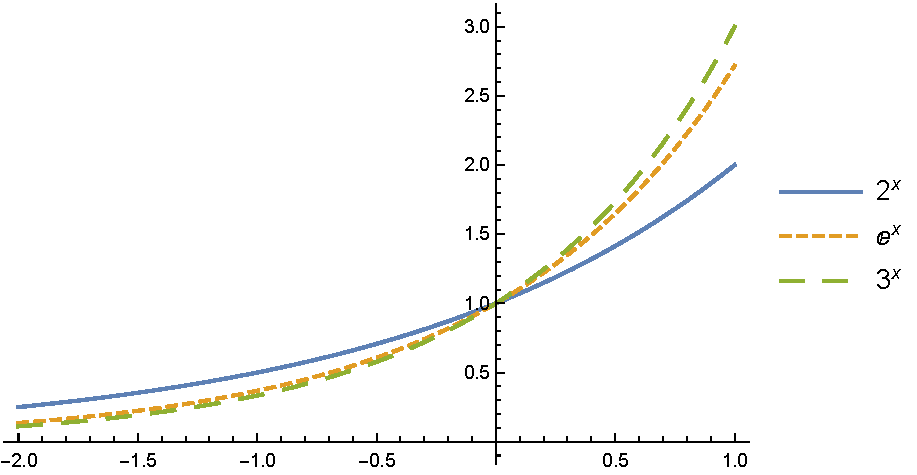
\includegraphics[width=0.6\textwidth]{Figures/expfunctions.pdf}
    \caption{Graphs of some exponential functions in the form $y = b^{x},b > 1$.}
    \label{f:expfunctions}
\end{figure}

\subsection{Logarithmic Functions}
Recall that a \textbf{function} is a relation between one set (domain) to another (range) such that for each $x$ in the domain there is exactly one $y = f(x)$. Also recall that a function is \textbf{one-to-one} if for every $a, b$ in the domain of $f$, $f(a) = f(b) \Rightarrow a = b$. This is equivalent to saying $a \neq b \Rightarrow f(a) \neq f(b)$, in other words, different things go in to $f$, different things come out. One-to-one functions are the only ones with \textbf{inverses}; these reverse the relation.

\begin{definition}\label{d:inverse-function}
    Let \(f\) be a one-to-one function. \textbf{Then the inverse of \(\bm{f}\)}, written \(f^{-1}\) \faFrown \ is defined as
    \[y = f^{-1}(x) \Leftrightarrow x = f(y)\]
\end{definition}
This basically switches the domain and range. The graph of $f^{-1}$ is the graph of $f$ mirrored about the line $y = x$.

Note that exponential functions are one-to-one! So they can have inverses!
\begin{definition}
    The \textbf{logarithm of \(\bm{x}\) base \(\bm{b}\)}, is defined as 
    \[y = \log_{b} x \Leftrightarrow x = b^{y}\]
\end{definition}
This means that $\log_{b} x$ is the power we need to put on $b$ to get $x$ as the result. Some example graphs are shown in Figure \ref{f:logfunctions}. Logarithmic functions have the following properties:
\begin{itemize}
    \item Domain: $(0, \infty)$; Range: $\mathbb{R}$
    \item Always increasing
    \item Vertical asymptote from the right at $x = 0$; note that as $x \to 0^{+}$, $\log_{b} x \to -\infty$
    \item As inverses, $\log_{b} b^{x} = x$ for $x \in \mathbb{R}$; $b^{\log_{b} x} = x$ for all $x > 0$
    \item $\log_{b} 1 = 0$ for all $b > 0$
\end{itemize}
One set of properties in particular, the \textbf{Laws of Logarithms}, will be of great help later:
\begin{itemize}
    \item $\log_{b} xy = \log_{b} x + \log_{b} y$
    \item $\log_{b} \frac{x}{y} = \log_{b} x - \log_{b} y$
    \item $\log_{b} x^{y} = y \log_{b} x$
\end{itemize}
The proof of the first is as follows: Let $u = \log_{b} x$ and $v = \log_{b} y$; then $x = b^{u}$ and $y = b^{v}$. Now $xy = b^{u}b^{v} = b^{u + v} \Rightarrow \log_{b} xy = u + v = \log_{b} x + \log_{b} y$. The others are similar.
We will almost always use $e$ as the base: $\log_{e} x = \ln x$, the \textbf{natural logarithm}.

\begin{figure}[htbp]
    \centering
        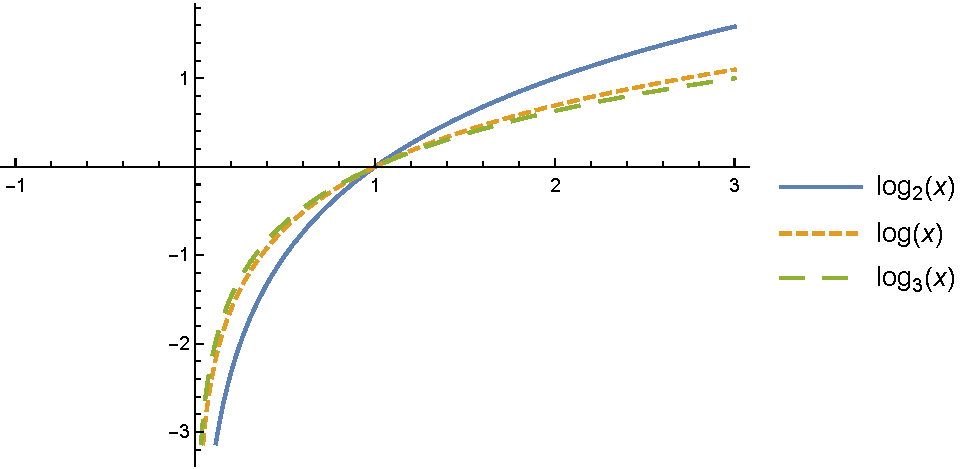
\includegraphics[width = 0.6\textwidth]{Figures/logfunctions.pdf}
    \caption{Graphs of some logarithmic functions in the form $y = \log_{b} x,b > 1$.}
    \label{f:logfunctions}
\end{figure}

\section{Inverse Trigonometric Functions}
\setcounter{figure}{0}
Trig functions are not 1-1! So how do we get inverses?! By restricting their domains! Note that $f(x) = \sin x$, $-\frac{\pi}{2} \leq x \leq \frac{\pi}{2}$ is 1-1 and covers the entire range. We can now define the \textbf{inverse trigonometric functions}:
\begin{itemize}
    \item $y = \sin^{-1} x \Leftrightarrow x = \sin y, -\frac{\pi}{2} \leq y \leq \frac{\pi}{2}$
    \item $y = \cos^{-1} x \Leftrightarrow x = \cos y, 0 \leq y \leq \pi$
    \item $y = \tan^{-1} x \Leftrightarrow x = \tan y, -\frac{\pi}{2} < y < \frac{\pi}{2}$
    \item $y = \sec^{-1} x \Leftrightarrow x = \sec y, 0 \leq y < \frac{\pi}{2}, \pi \leq y < \frac{3\pi}{2}$
\end{itemize}
Inverse secant, cosecant, and cotangent functions are rarely ever used. We are not going to worry about the graphs (shown in Figure \ref{f:invtrigfunctions}) too much with one exception: take note of the inverse tangent graph and the horizontal asymptotes at \(y = \pm \frac{\pi}{2}\).
\begin{figure}[htbp]
    \centering
        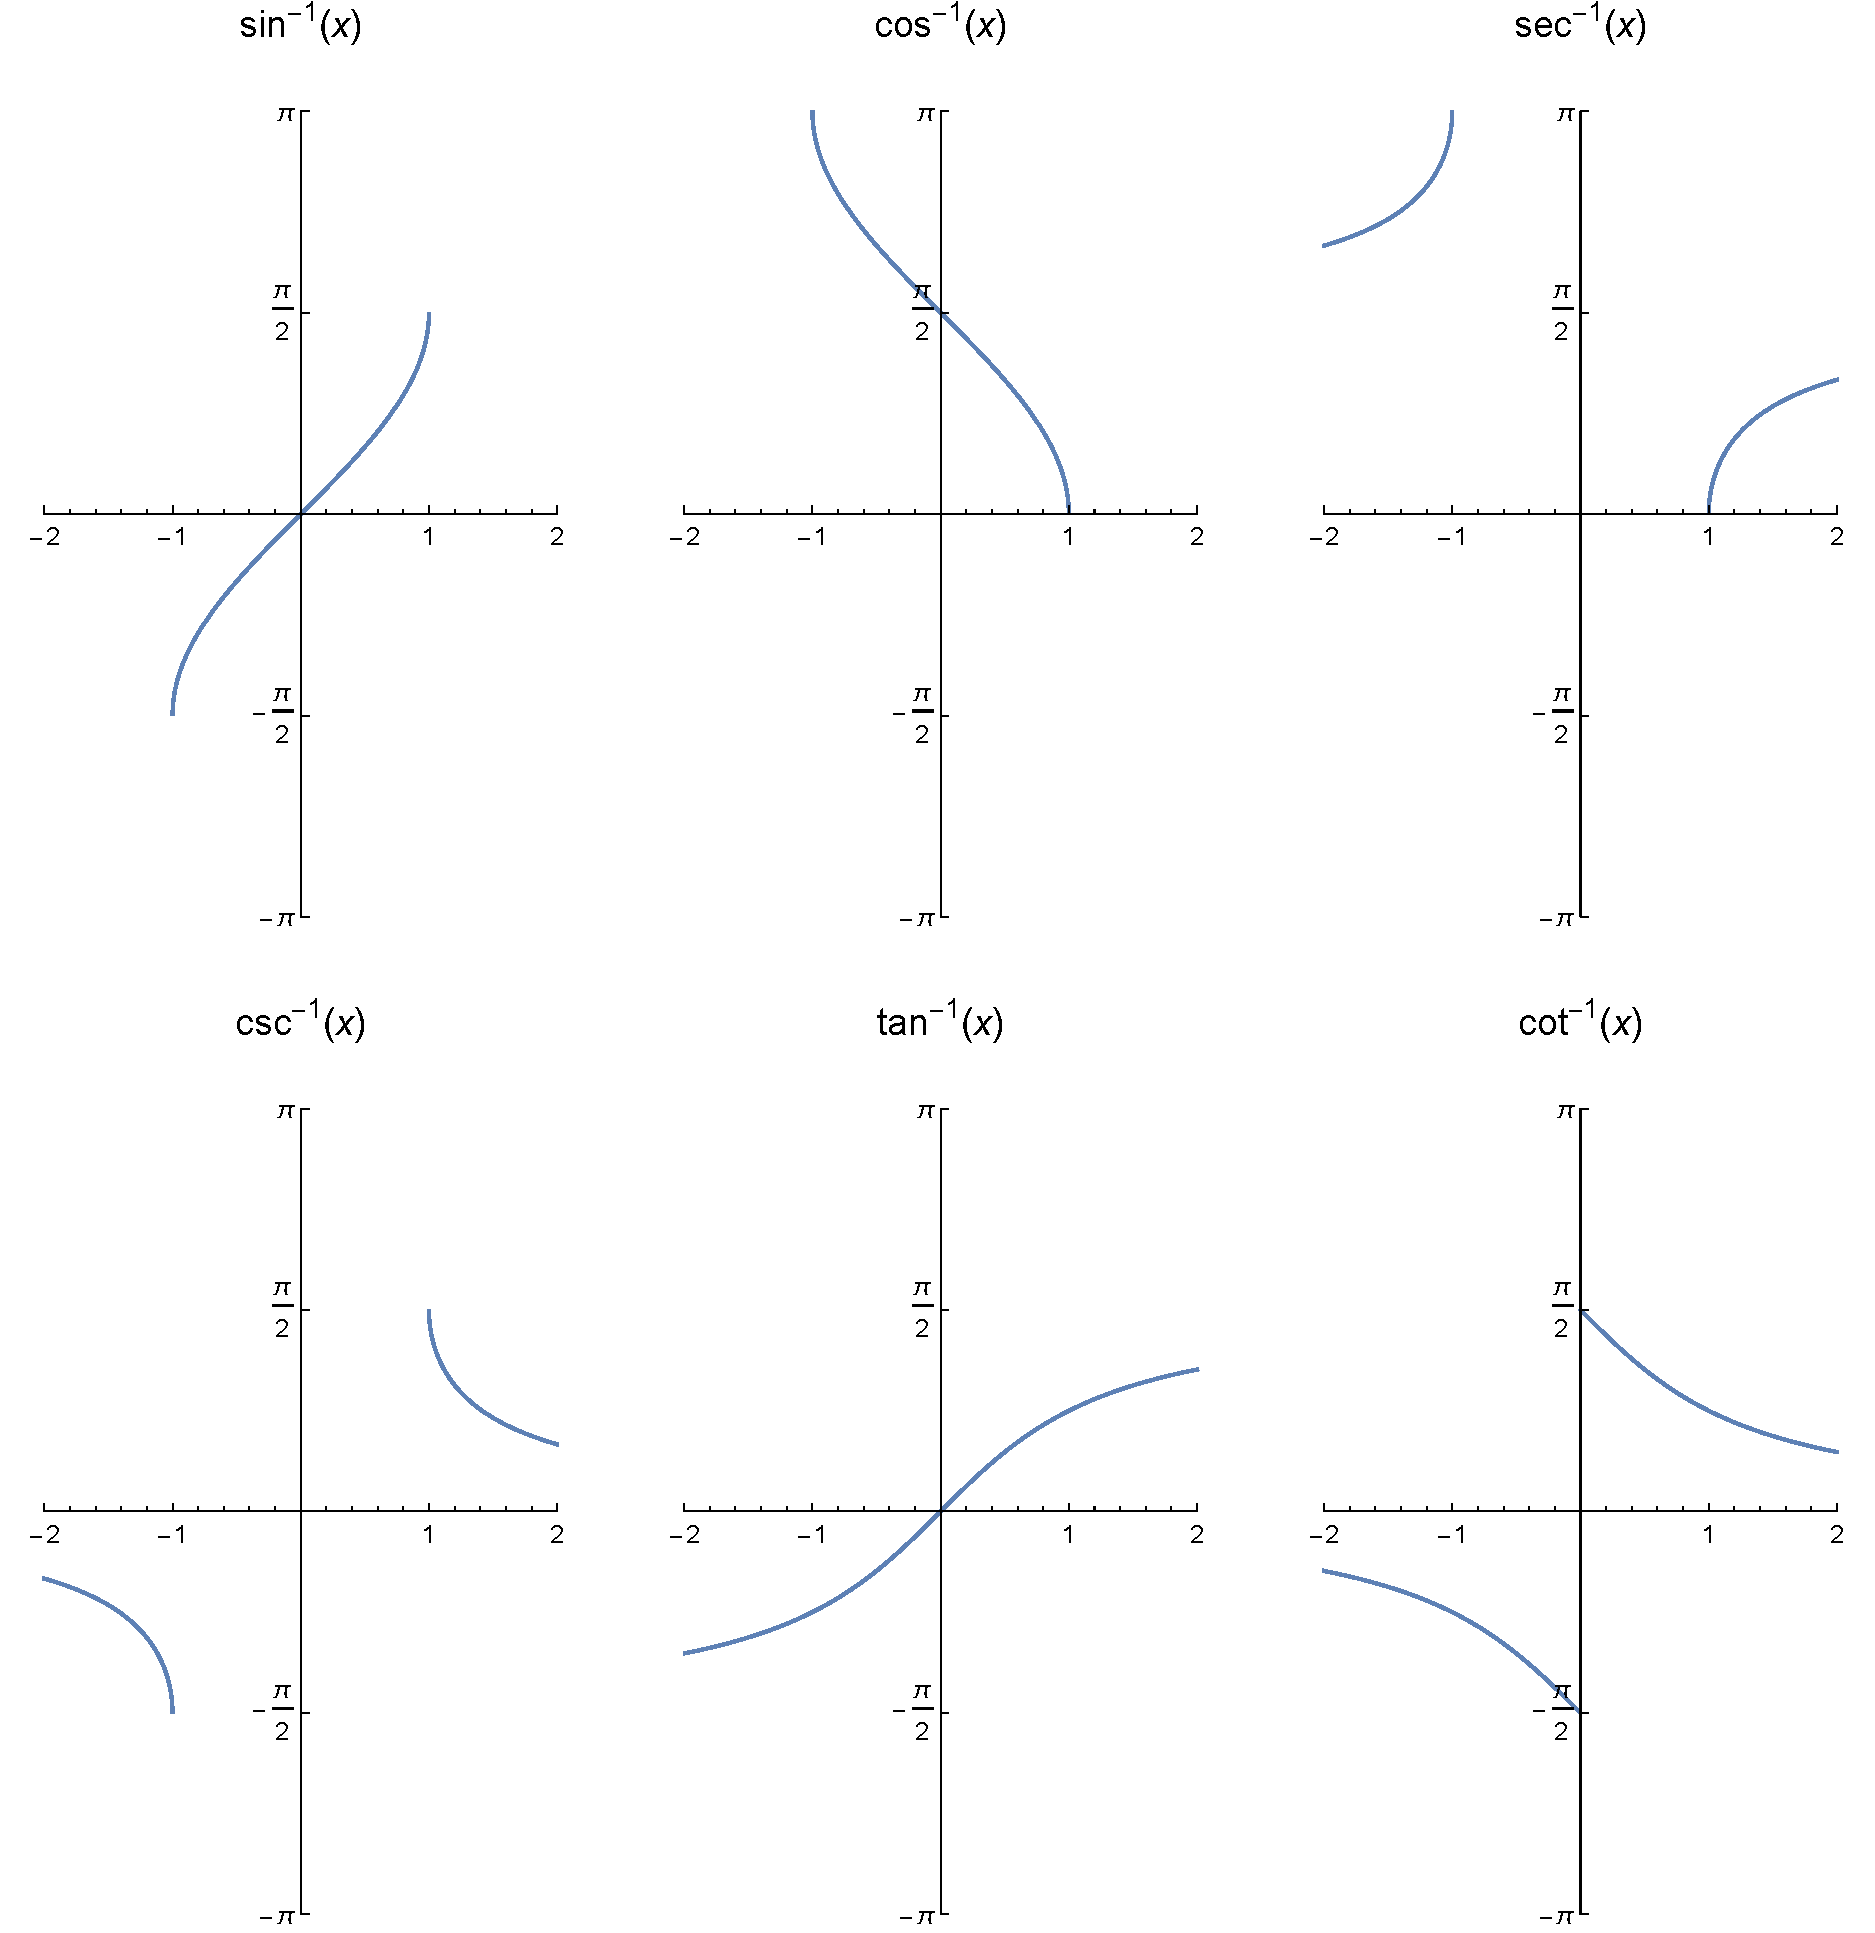
\includegraphics[width=\textwidth]{Figures/invtrigfunctions.pdf}
    \caption{Graphs of the Inverse Trigonometric Functions.}
    \label{f:invtrigfunctions}
\end{figure}

\newpage\thispagestyle{firstofchapter}
\chapter{Limits and Derivatives}
\section{Definition of a Limit}
\setcounter{figure}{0}

\begin{itemize}
    \item Let's look at $\displaystyle f(x) = \frac{x^{2} - 4}{x - 2}$
    \item For all $x \neq 2, f(x) = x + 2$; when $x = 2$ we just have a hole in the graph.
    \item When $x$ gets very close to 2, though, the values of $f(x)$ can be made arbitrarily close to 4. See figure \ref{f:deflimitplot} below.
    \item This shows the idea of a limit
\end{itemize}

\begin{definition}\label{d:limit}
    We say the \textbf{limit as $\bm{x}$ approaches $\bm{a}$ is $\bm{L}$}, written
    \[
        \lim_{x \to a} f(x) = L  
    \]
    if we can make $f(x)$ as close as we want to $L$ by making $x$ close enough (but not equal to) $a$.
\end{definition}

\begin{itemize}
    \item This is not the \textit{formal} definition of a limit but it's fine for us \faSmile
    \item Formal definition:
    \[
        \lim_{x \to a} f(x) = L \Leftrightarrow \forall \epsilon > 0, \exists \delta > 0, 0 < | x - a | < \delta \Leftarrow | f(x) - L | < \epsilon \text{ \faMeh} 
    \]
    \item This is mostly useful for math majors but take it from me, you will have forgotten by the time you need it again anyway \faSmile
    \item For now we will evaluate limits by looking at their graphs but in the next section we will introduce limit laws to evaluate given the function
\end{itemize}

\begin{figure}[htbp]
    \centering
        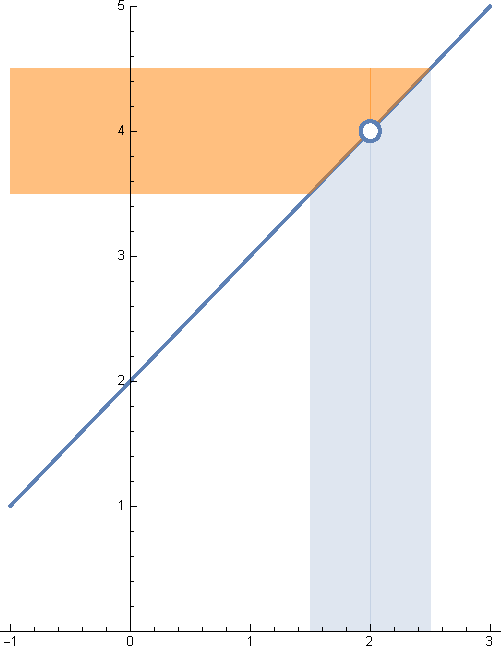
\includegraphics[width=0.4\textwidth]{Figures/deflimitplot.pdf}
    \caption{Graph and intervals for function $f(x) = \dfrac{x^{2} - 4}{x - 2}$.}
    \label{f:deflimitplot}
\end{figure}

\subsection{Infinite Limits}
\setcounter{figure}{0}

\begin{itemize}
    \item When the limit has the form of $\frac{\text{Not zero}}{0}$ the limit does not exist
    \item But can we say more?
    \item Vertical asymptotes are the most common way we will see limits not existing
\end{itemize}
\begin{definition}\label{d:infinite-limit}
    We say that \textbf{the limit as $\bm{x}$ approaches $\bm{a}$ is infinity}, written
    \[
        \lim_{x\to a} f(x) = \infty
    \]    
    if we can make $f(x)$ as large and positive as we want by making $x$ close enough (but not equal) to $a$.
\end{definition}
\begin{itemize}
    \item Do not try to find these by plugging in; think analytically
    \item What does the numerator approach? Positive or negative?
    \item From which direction does the denominator approach zero?
\end{itemize}

\begin{example}\label{e:inf-limit-one-side}
    Evaluate $\displaystyle \lim_{x \to 2^{-}} \frac{x+4}{x-2}$.
    \begin{solution}
        This limit initially has a form of $\frac{6}{0}$ (\emph{but is not equal to} $\frac{6}{0}$). This means it does not exist. But also we note that the numerator approaches 6 (which is positive) while the denominator approaches 0 through negative values. So we say the limit is equal to $-\infty$.
    \end{solution}
\end{example}

\begin{example}\label{e:inf-limit-one-side-2}
    Evaluate \( \displaystyle \lim_{x \to -1^{+}} \frac{2x}{x^{2} - 1} \).
    \begin{solution}
        The numerator approaches \(-2\); for the denominator, since \(x\) is approaching \( -1\) from the right, we have \(-1 < x < 0\) which means \(x^{2} < 1 \Rightarrow x^{2} - 1 < 0\) so the denominator approaches 0 through negative values. Thus the limit is equal to \(\infty\).
    \end{solution}
\end{example}

\section{Limit Laws}
\setcounter{figure}{0}

\subsection{Some Rules to Help Evaluate Limits}
\begin{itemize}
    \item Do not worry about memorizing these because memorization and math do not mix anyway
    \item We are mostly concerned with their application
    \begin{enumerate}
        \item $\displaystyle \lim_{x \to a} (f(x) + g(x)) = \lim_{x \to a} f(x) + \lim_{x \to a} g(x)$ (same for subtraction)
        \item $\displaystyle \lim_{x \to a} f(x)g(x) = \left( \lim_{x \to a} f(x) \right) \left( \lim_{x \to a} g(x) \right)$
        \item $\displaystyle \lim_{x \to a} \frac{f(x)}{g(x)} = \frac{\displaystyle \lim_{x \to a} f(x)}{\displaystyle \lim_{x \to a} g(x)}$ provided $\displaystyle \lim_{x \to a} g(x) \neq 0$
        \item $\displaystyle \lim_{x \to a} \left[ f(x) \right]^{n} = \left[ \lim_{x \to a} f(x) \right]^{n}$
        \item $\displaystyle \lim_{x\to a} \sqrt[n]{f(x)}  = \sqrt[n]{\lim_{x\to a} f(x)}$ assuming no negatives under roots, etc.
        \item $\displaystyle \lim_{x\to a} x = a$ \faMeh \; This really does require a proof though!
        \item $\displaystyle \lim_{x\to a} c = c$ \faMeh \; Again, seems obvious but there is a proof!
    \end{enumerate}
    \item We will look at others as we go but this is good for now
    \item Need not cite these step-by-step but will do one example with them step-by-step
\end{itemize}

\begin{example}\label{e:limit-justplugin}
    Evaluate $\displaystyle \lim_{x\to 2} \left( x^{2} + 3x - 4 \right)$.   
    \begin{solution}
        Here we go \faMeh
        \begin{align*}
            \lim_{x\to 2} \left( x^{2} + 3x - 4 \right)     &= \lim_{x\to 2} x^{2} + \lim_{x\to 2} 3x - \lim_{x\to 2} 4\\
                                                            &= \left(\lim_{x\to 2} x\right)^{2} + 3\lim_{x\to 2} x - 4\\
                                                            &= 2^2 + 3\cdot 2 - 4\\
                                                            &= 6
        \end{align*}
    But what did we just end up doing? Just plugging in 2 for $x$! \faMeh
    \end{solution}    
\end{example}
\begin{itemize}
    \item So these limit laws say if we have an algebraic function we should just try plugging in $a$ for $x$
    \item As long as we get a real number out of it we are good \faSmile
    \item But what if we are not, say, if we divide by zero? 
\end{itemize}
\subsection{Dividing by Zero and Indeterminate Forms}
\begin{itemize}
    \item If we plug in $a$ for $x$ and get any of the following: $\frac{0}{0}$, $\infty - \infty$, $\frac{\infty}{\infty}$, $1^{\infty}$, $0^{0}$, or $\infty^{0}$, we have an \textbf{indeterminate form}.
    \item This means that it depends on whether one function is moving significantly faster than the other
    \item May have to do one of many things to sort it out
    \item Will develop other techniques later
    \item If the limit has the form $\frac{\text{Not zero}}{0}$ the limit does not exist (DNE)
    \item Will go more into infinite limits in a later section
    \item[{\faExclamationTriangle[solid]}] Never ever say a limit is equal to any indeterminate form
\end{itemize}

\begin{example}\label{e:limit-factoring}
    Evaluate $\displaystyle \lim_{x\to -1} \frac{x^{2} -4x  -5}{x^{2} - 1}$ or show that it does not exist.
    \begin{solution}
        Plugging in gives the $\frac{0}{0}$ indeterminate form. Note that we can factor both the numerator and denominator:
        \begin{align*}
            \lim_{x\to -1} \frac{x^{2} -4x  -5}{x^{2} - 1}  &= \lim_{x\to -1} \frac{(x+1)(x-5)}{(x-1)(x+1)}\\
                                                            &= \lim_{x\to -1} \frac{x - 5}{x - 1}\\
                                                            &= \frac{-1 - 5}{-1 -1} = 3
        \end{align*}
    \end{solution}
    \begin{commentary}
        \faExclamationTriangle[solid] \; Note that we use "$\displaystyle \lim_{x\to -1}$" at every step until we can safely plug in
    \end{commentary}
\end{example}

\begin{example}\label{e:limitrationalize}
    Evaluate $\displaystyle \lim_{x\to 3} \frac{\sqrt{x + 13} - 4}{x - 3}$ or show that it does not exist.
    \begin{solution}
        This limit has the $\frac{0}{0}$ indeterminate form. We need to rationalize the numerator first, then combine some terms, then cancel. Then we can evaluate by plugging in.
        \begin{align*}
            \lim_{x\to 3} \frac{\sqrt{x + 13} - 4}{x - 3}   &= \lim_{x\to 3} \frac{\sqrt{x + 13} - 4}{x - 3} \cdot \frac{\sqrt{x + 13} + 4}{\sqrt{x + 13} + 4} \\
                                                            &= \lim_{x\to 3} \frac{(x + 13) - 16}{(x-3)\left( \sqrt{x + 13} + 4 \right)}\\
                                                            &= \lim_{x\to 3} \frac{x - 3}{(x-3)\left( \sqrt{x + 13} + 4 \right)}\\
                                                            &= \lim_{x\to 3} \frac{1}{ \sqrt{x + 13} + 4} = \frac{1}{\sqrt{3 + 13} + 4} = \frac{1}{8}
        \end{align*}
    \end{solution}
    \begin{commentary}
        Note that we do not expand the denominator; this would hide the factor $(x - 3)$ that we want to cancel.
    \end{commentary}
\end{example}

\begin{example}\label{e:limit-rational-functions}
    Evaluate $\displaystyle \lim_{x\to -2} \frac{\frac{1}{x - 2} + \frac{1}{4}}{x + 2}$ or show that it does not exist.
    \begin{solution}
        This limit has the $\frac{0}{0}$ indeterminate form. We will clear out the little denominators by multiplying through by the LCD:
        \begin{align*}
            \lim_{x\to -2} \frac{\frac{1}{x - 2} + \frac{1}{4}}{x + 2}  &= \lim_{x\to -2} \frac{\left(\frac{1}{x - 2} + \frac{1}{4}\right)}{x + 2} \cdot \frac{4(x - 2)}{4(x - 2)} \\
                                                                        &= \lim_{x\to -2} \frac{4 + (x-2)}{4(x-2)(x+2)} = \lim_{x\to -2}\frac{x + 2}{4(x-2)(x+2)}\\
                                                                        &= \lim_{x\to -2} \frac{1}{4(x-2)} = \frac{1}{4(-4)} = -\frac{1}{16}
        \end{align*} 
    \end{solution}
    \begin{commentary}
        Note that you can also combine the little quotients in the "main" numerator to get the same result.
    \end{commentary}
\end{example}
Sometimes we need a limit with a function involving the absolute value function.
\begin{definition}\label{d:abs-val}
    The \textbf{absolute value} of \(x, |x| \), is the distance from \(x\) to 0 on the real number line. Equivalently,
    \[ |x| = 
    \begin{cases}
        \phantom{-}x \; &\text{ if } x \ge 0\\
        -x \; &\text{ if } x < 0
    \end{cases}
    \]
\end{definition}
We can adjust this for other expressions.

\begin{example}\label{e:limit-absval}
    Evaluate \(\displaystyle \lim_{x \to 3^{-}} \frac{|x^{2} - 3x|}{x^{2}-9}\).
    \begin{solution}
        Use the fact that when \(x<3\), \(|x-3| = -(x-3)\):
        \[\lim_{x \to 3^{-}} \frac{|x^{2} - 3x|}{x^{2}-9} = \lim_{x \to 3^{-}} \frac{|x||x-3|}{(x-3)(x+3)} = \lim_{x \to 3^{-}} -\frac{|x|(x-3)}{(x-3)(x+3)} = \lim_{x \to 3^{-}} -\frac{|x|}{x+3} = -\frac{1}{2}\]
    \end{solution}
\end{example}

\subsection{The Squeeze Theorem}

\begin{theorem}[The Squeeze Theorem]\label{t:squuezethm}
    Suppose that \(f(x) \leq g(x) \leq h(x)\) when \(x\) is near \(a\) and \(\displaystyle \lim_{x \to a} f(x) = \lim_{x \to a} h(x) = L\). Then \(\displaystyle \lim_{x \to a} g(x) = L\).
\end{theorem}
\begin{figure}[htbp]
    \centering
        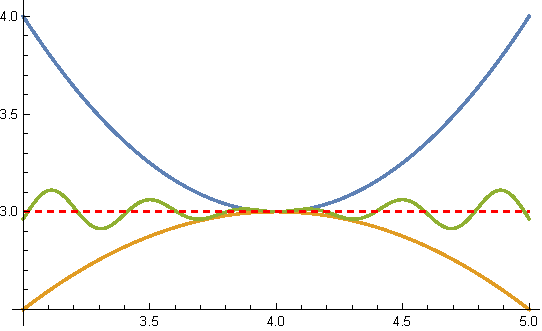
\includegraphics[width=0.4\textwidth]{Figures/squeezethm.pdf}
    \caption{Middle function is squeezed through the bottleneck.}
    \label{f:squeeze-thm}
\end{figure}
\begin{commentary}
    We will not use this for much directly but it will be helpful occasionally.
\end{commentary}

\section{Limits at Infinity}
\setcounter{figure}{0}

\begin{itemize}
    \item Calculus books always do this the hard way \faFrown
    \item We will do these the easy way \faSmile
\end{itemize}
\begin{definition}\label{d:limit-to-infty}
    We say the \textbf{limit as $\bm{x}$ approaches infinity of $\bm{f}$ is $\bm{L}$}, written
    \[
        \lim_{x \to \infty} f(x) = L    
    \]
    if we can make $f(x)$ as close as we want to $L$ by making $x$ large enough and positive.
\end{definition}
\subsection{Rational Functions}

\begin{itemize}
    \item These are nice; basic idea is to only look at dominant terms
    \item May use fact that \(\displaystyle \lim_{x \to \infty} \frac{1}{x^{n}} = 0, n \in \mathbb{Q}\)
    \item Dominant terms are only ones that matter, ignore everything else
\end{itemize}
\begin{example}\label{e:lim-at-inf-rational}
    Evaluate each limit.
    \begin{enumerate}
        \item \(\displaystyle \lim_{x \to \infty} \frac{x^{3} - 2x^{2} + 5}{4 x^{3}- x + 2} = \frac{1}{4}\)
        \item \(\displaystyle \lim_{x \to \infty} \frac{3x}{x^{3} - 1} = 0\)
        \item \(\displaystyle \lim_{x \to -\infty} \frac{1-x^{5}}{1+ x^{2}} = \infty\)
    \end{enumerate}
\end{example}

\subsection{Other Functions}
Can adapt idea of dominant terms to other functions
\begin{example}\label{e:lim-at-inf-algebraic}
    Evaluate each limit.
    \begin{enumerate}
        \item \(\displaystyle \lim_{x \to \infty} \frac{x}{\sqrt{x^{2} + 1}} = 1\)
        \item \(\displaystyle \lim_{x \to -\infty} \frac{x}{\sqrt{x^{2} + 1}} = -1\)
        \item  \(\displaystyle \lim_{x \to -\infty} \left(x + \sqrt{x^{2} - 3x}\right)\)
        \begin{solution}
            For this one we need to rationalize the numerator. What numerator? We make one! \faSmile \, So we get:
            \begin{align*}
                \lim_{x \to -\infty} \left(x + \sqrt{x^{2} - 3x}\right) &= \lim_{x \to -\infty} \left(x + \sqrt{x^{2} - 3x}\right) \cdot \frac{x - \sqrt{x^{2} - 3x}}{x - \sqrt{x^{2} - 3x}} \\
                                                                &= \lim_{x \to -\infty} \frac{x^{2} - (x^{2} - 3x)}{x - \sqrt{x^{2} - 3x}}\\
                \intertext{combining like terms and eliminating the non-dominant term in the denominator, we get:}
                                                                &= \lim_{x \to -\infty} \frac{3x}{x - \sqrt{x^{2}}}\\
                                                                &= \lim_{x \to -\infty} \frac{3x}{2x}\\
                                                                &= \frac{3}{2}
            \end{align*}
        \end{solution}
    \end{enumerate}
\end{example}
\section{Continuity}
\setcounter{figure}{0}

\begin{definition}\label{d:continuity}
    A function is \textbf{continuous at} \(\bm{a}\) if
    \[\lim_{x \to a} f(x) = f(a)\]
\end{definition}
Note that this means that the function must be defined at \(a\), the limit as \(x\) approaches \(a\) must exist, and the two must be equal.

If f and g are continuous at a, so are:
\begin{multicols}{2}
    \begin{itemize}
        \item \(f + g\)
        \item \(f - g\)
        \item \(fg\)
        \item \(f/g\) (provided that \(g(a) \neq 0\))
        \item \(f \circ g\)
    \end{itemize}
\end{multicols}

Note that with composition of functions, this means that if \(g\) is continuous at \(a\) and \(f\) is continuous at \(g(a)\) then \(f(g(x))\) is continuous at \(a\); this means that \(\displaystyle \lim_{x\to a} f(g(x)) = f\left(\lim_{x \to a} g(x) \right) = f(g(a))\).

A function is continuous on an interval if it is continuous at every point in the interval. These functions are continuous everywhere they are defined:
\begin{multicols}{2}
    \begin{itemize}
        \item Polynomials
        \item Rational functions
        \item Constant functions
        \item Trigonometric
        \item Inverse Trigonometric
        \item Exponential
        \item Logarithmic
        \item Root functions
    \end{itemize}
\end{multicols}

Continuity is also preserved through inverses as well.

\begin{example}
    Find the values \(a\) and \(b\) that make the function below continuous.
    \[f(x)= \begin{cases}
        -\frac{1}{x} &\text{ if } x < -1\\
        a x^2 + bx - 1 &\text{ if } -1 \leq x < 2\\
        x + a + b + 3 &\text{ if } x \geq 2
    \end{cases}\]
    \begin{solution}
        Setting limits from the left and right of \(-1, 2\) equal we get the following system of equations:
        \begin{align*}
            a - b &= 2\\
            3a + 6 &= 6
        \end{align*}
        which has the solution \(a=2, b=0\).
    \end{solution}
\end{example}

\subsection{The Intermediate Value Theorem}
We won't use this directly much but still important!
\begin{theorem}[Intermediate Value Theorem]\label{t:int-val-thm}
    Suppose \(f\) is continuous on \([a,b]\) and \(L\) is any number strictly between \(f(a)\) and \(f(b)\). Then there exists a \(c \in (a,b)\) such that \(f(c) = L\).
\end{theorem}
This makes sense; with continuity we have the cross the line \(y = L\) at some point (and that's the \(c\) mentioned in the theorem).

\begin{example}
    Use the Intermediate Value Theorem to show that there is a solution to the equation \(x e^x = 1\) in the interval \(\left[0, 1\right]\).
    \begin{solution}
        Let \(f(x) = x e^x\). Now \(f(0) = 0 < 1 < f(1) = e\); since \(f\) is continuous for all \(x\), it satisfies the conditions of the Intermediate Value Theorem, so there must be a value \(c\) in \((0,1)\) where \(f(c) = 1\). Note that this function cannot be solved for \(x\) in an exact form, but can be solved numerically to get \(x \approx 0.567143\).
    \end{solution}
\end{example}

\section{Definition of the Derivative}

Now it is time for the first big problem in calculus: the Tangent Problem!
\begin{itemize}
    \item Want to find the slope of the tangent line to the graph of \(y = f(x)\) at the point \( T(x, f(x))\)
    \item But we need two points for slope; to get another point we need the equation of the line; to get the equation we need the slope \faFrown
    \item But now we have calculus and limits! \faSmile
    \item Take another point on the graph at \(S(x+h, f(x+h))\) and form the \textbf{secant line} \(\overline{ST}\). See Figure \ref{f:tan-sec-lines}.
    \item Initially not that good \faFrown \, but if we move the second point closer and let \(h \to 0\) the approximation becomes exactly what we want \faSmile
    \item Define the slope of the tangent line to be the limit of the slope of the secant line as \(h \to 0\)
    \item We will let \(x\) stay a variable; note that this limit does not change \(x\) so the result (if it exists) will be a new function of \(x\)
    \item We call this new function \textbf{the derivative of \(\bm{f}\) with respect to \(\bm{x}\)}, \(f'(x)\).
\end{itemize}
\begin{definition}\label{d:derivative}
    \textbf{The derivative of \(\bm{f}\) with respect to \(\bm{x}\)} is
    \[f'(x) = \lim_{h \to 0} \frac{f(x+h) - f(x)}{h}\]
\end{definition}
\begin{itemize}
    \item More generally this is the rate of change in the function
    \item Finding \(f'(x)\) using the definition is a pain for even easy functions \faFrown \, but we will see shortcuts soon \faSmile
\end{itemize}
\begin{figure}[htbp]
    \centering
        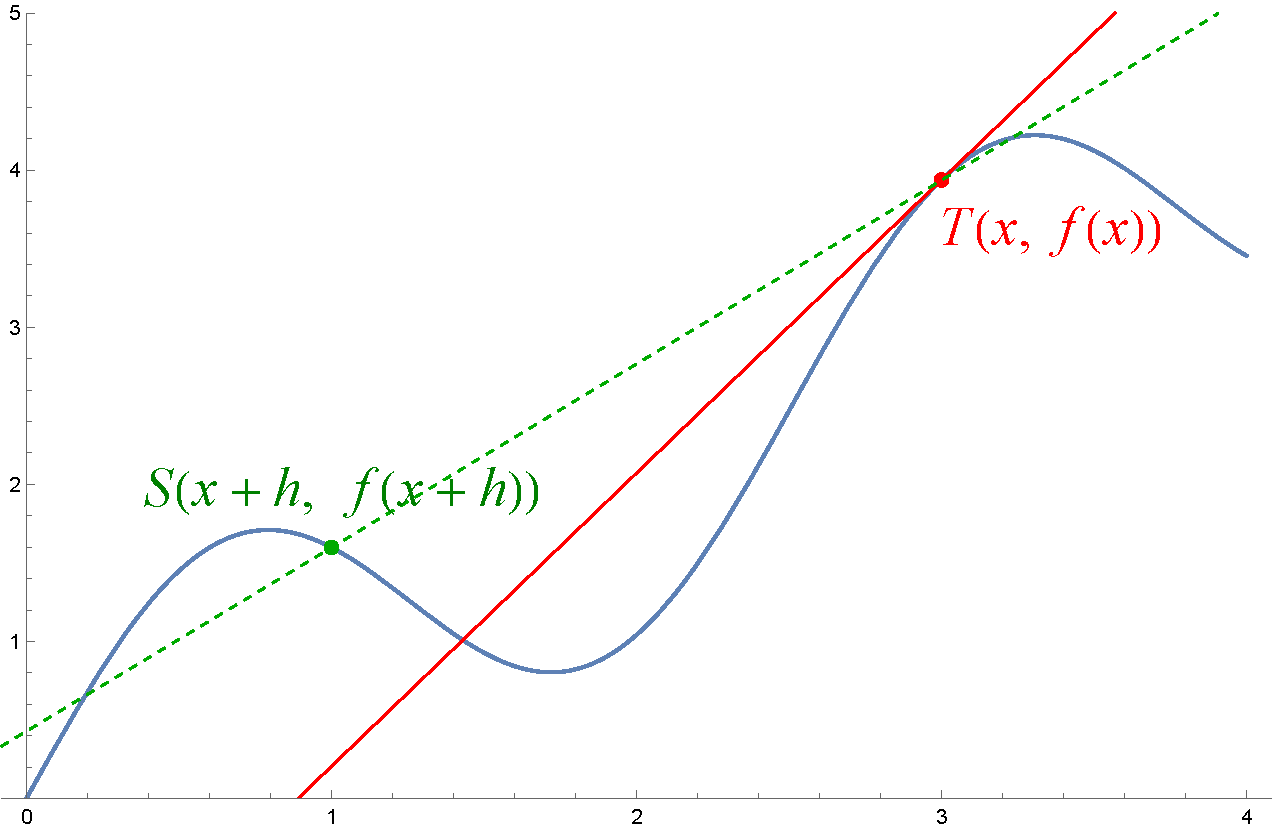
\includegraphics[width=0.4\textwidth]{Figures/tangentline.pdf}
    \caption{Curve with tangent line at point \(T\) and secant line \(\overline{ST}\).}
    \label{f:tan-sec-lines}
\end{figure}

\begin{example}\label{e:def-deriv-parabola}
    Find the derivative of \(f(x) = x^{2}\) then find the slope-intercept equation of the tangent line at the point \((2,4)\).
    \begin{solution}
        \begin{align*}
            f'(x)   &= \lim_{h \to 0} \frac{(x+h)^{2} - x^{2}}{h} = \lim_{h \to 0} \frac{x^{2} + 2xh + h^{2} - x^2}{h} \\
                    &= \lim_{h \to 0} \frac{2xh + h^{2}}{h} = \lim_{h \to 0} (2x + h) = 2x
        \end{align*}
    Now the slope of the tangent line is \(m = f'(2) = 4\); the point-slope form of the line is \(y - 4 = 4(x-2) \Rightarrow y = 4x - 4\).
    \end{solution}
\end{example}

\begin{example}\label{e:def-deriv-rational}
    Find the derivative of \(\displaystyle f(x) = \frac{x+1}{x-3}\).
    \begin{solution}
        \begin{align*}
            f'(x)   &= \lim_{h \to 0} \left(\frac{x+h+1}{x+h-3} - \frac{x+1}{x-3}\right)\cdot \frac{1}{h} \\
                    &= \lim_{h \to 0} \frac{(x+h+1)(x-3) - (x+1)(x+h-3)}{h(x+h-3)(x-3)} = \lim_{h \to 0} \frac{-4h}{h(x+h-3)(x-3)}\\
                    &= {-}\frac{4}{(x+3)^{2}}
        \end{align*}
    \end{solution}
\end{example}

\subsection{Higher Order Derivatives}
The derivative of a function gives us a new function. So who says we cannot take the derivative of a derivative? Nobody! \faSmile \ We can define the \textbf{second derivative} as \(f''(x) = \frac{d}{dx}f'(x)\). Why stop now? The third derivative is \(f'''(x) = \frac{d}{dx}f''(x)\). We can keep going! But usually once we get to the fourth derivative, we use \(f^{(4)}(x)\) because nobody wants to count all those primes.

We will do more with higher order derivatives once we see more efficient ways of finding them.

\begin{itemize}
    \item Other notation for derivative: \(f'(x) = y' = \frac{dy}{dx} = \frac{d}{dx}f(x) = D_{x} f(x) \)
    \item Differentiability implies continuity (but not other way; sharp points, vertical tangents)
\end{itemize}
\newpage\thispagestyle{firstofchapter}
\chapter{Derivative Rules}
\section{Basic Derivative Rules}
\begin{itemize}
    \item \( \frac{d}{dx} c = 0\) for any constant \(c\)
    \item (Power Rule) \(\frac{d}{dx} x^{n} = n x^{n-1}\) for all real \(n\)
    \begin{itemize}
        \item We will do a proof of this later; need some other tools first
        \item Proof for now in most texts only works for positive integers \(n\) and is messy
    \end{itemize}
\end{itemize}
\begin{example}\label{e:power-rule-basic}
    Find the derivative of each function.
    \begin{enumerate}
        \item \(f(x) = x^{5} \Rightarrow f'(x) = 5x^{4}\)
        \item \(f(x) = \sqrt{x} \Rightarrow f'(x) = \frac{1}{2}x^{-1/2}\)
        \item \(f(x) = \frac{1}{x^{6}} = x^{-6} \Rightarrow f'(x) = -6x^{-7} = -\frac{6}{x^{7}}\)
        \item \(f(x) = x  \Rightarrow f'(x) = 1\cdot x^{0} = 1\)
    \end{enumerate}
\end{example}
\begin{itemize}
    \item For any differentiable functions \(f\) and \(g\), \(\frac{d}{dx}\left(f(x) + g(x)\right) = f'(x) + g'(x)\)
    \item \(\frac{d}{dx} c f(x) = cf'(x)\)
    \item Now we can take derivatives of polynomials and more!
\end{itemize}

\begin{example}
    \begin{align*}
        f(x) = 4x^{3} - \tfrac{2}{3}x^{6} &\Rightarrow f'(x) = 12x^{12} - 4x^{5}\\
        f(x) = \frac{x^{4} + 6x - 1}{x} &\Rightarrow f'(x) = 3x^{2} + x^{-2}\\
        f(x) = (4x+1)(3x-2) = 12x^{2} - 5x - 2 &\Rightarrow f'(x) = 24x - 5
    \end{align*}
\end{example}

Earlier we defined Euler's number e as the value for which \(\displaystyle \lim_{h \to 0} \frac{e^{h} - 1}{h} = 1\). Now we can define the derivative of \(e^{x}\):

\[\frac{d}{dx} e^{x} = \lim_{h \to 0} \frac{e^{x+h} - e^{x}}{h} = e^{x} \lim_{h \to 0} \frac{e^{h} - 1}{h} = e^{x} \cdot 1 = e^{x}\]

My favorite derivative rule! \faSmile \, \faHeart

\section{Product and Quotient Rules}

\begin{theorem}[Product Rule]\label{t:product-rule}
    \(\dfrac{d}{dx} f(x)g(x) = f(x)g'(x) + g(x)f'(x)\)
\end{theorem}
Proof later! Much easier that way with Logarithmic Differentiation \faSmile \, Though right now there is not much we can do with this \faMeh

\begin{example}
    \begin{alignat*}{2}
        &f(x) = (x^{2} + 1)(4x-3)       &&\Rightarrow f'(x) = 2x(4x-3) + 4(x^{2} + 1) = 12x^{2} -6x + 4\\
        &f(x) = e^{x}(x^{3} + x + 1)    &&\Rightarrow f'(x) = e^x \left(x^3+3 x^2+x+2\right)
    \end{alignat*}
\end{example}


\begin{theorem}[Quotient Rule]\label{t:quotient-rule}
    \(\displaystyle \frac{d}{dx} \frac{f(x)}{g(x)} = \frac{g(x)f'(x) - f(x)g'(x)}{[g(x)]^{2}}\)
\end{theorem}
Again proof later

\begin{example}
    \begin{alignat*}{2}
        &f(x) = \frac{2x+1}{5x-3} &&\Rightarrow f'(x) = -\frac{11}{(5 x-3)^2}\\
        &f(x) = \frac{e^{x}}{e^{x} + 1} &&\Rightarrow f'(x) = \frac{e^x}{\left(e^x+1\right)^2}\\
        &f(x) = \frac{x^4-2 x-3}{x} &&\Rightarrow f'(x) = \frac{3 \left(x^4+1\right)}{x^2}\\
        &f(x) = \frac{\sqrt{x}}{x + 1} &&\Rightarrow f'(x) = \frac{1-x}{2 \sqrt{x} (x+1)^2}
    \end{alignat*}
\end{example}

\section{Derivatives of Trigonometric Functions}

\begin{itemize}
    \item Will need some special limits for proofs
    \item \(\displaystyle \lim_{x \to 0} \frac{\sin x}{x} = 1; \lim_{x \to 0} \frac{\cos x - 1}{x} = 0\)
    \item Will not prove these here
\end{itemize}

\begin{theorem}
    \(\dfrac{d}{dx} \sin x = \cos x\)
\end{theorem}
\begin{proof}
    \begin{alignat*}{2}
        \frac{d}{dx} \sin x     &= \lim_{h \to 0} \frac{\sin(x+h) - \sin x}{h} = \lim_{h \to 0} \frac{\sin(x+h) - \sin x}{h}\\
                                &= \lim_{h \to 0} \frac{\sin x \cos h + \sin h \cos x - \sin x}{h}\\
                                &= \lim_{h \to 0} \sin x\left(\sin x\frac{\cos h - 1}{h} + \frac{\sin h \cos x}{h}\right)\\
                                &= \cos x
    \end{alignat*}
\end{proof}
\begin{commentary}
    Proof for \(\frac{d}{dx} \cos x = -\sin x\) can be found similarly, then quotient rule for all others!
\end{commentary}

Here they are!
\begin{align*}
    \frac{d}{dx} \sin x &= \cos x           & \frac{d}{dx} \cos x &= -\sin x\\
    \frac{d}{dx} \tan x &= \sec^{2} x       & \frac{d}{dx} \cot x &= -\csc^{2} x\\
    \frac{d}{dx} \sec x &= \sec x \tan x    & \frac{d}{dx} \csc x &= -\csc x \cot x
\end{align*}
Just use these in the right place in the rule you are using.

\begin{example}
    \begin{alignat*}{2}
        &f(x) = x^{2}\cos x &&\Rightarrow f'(x) = 2x \cos x - x^{2}\sin x\\
        &f(x) = \frac{\tan x}{e^{x}} &&\Rightarrow f'(x) = \frac{\sec^{2}x - \tan x}{e^{x}}\\
        &f(x) = 2\csc x &&\Rightarrow f'(x) = -2\csc x \cot x
    \end{alignat*}
\end{example}

\section{Chain Rule}

This is where things really open up!

\begin{theorem}[Chain Rule]\label{t:chain-rule}
    \[\frac{d}{dx} f(g(x)) = f'(g(x))g'(x)\]
\end{theorem}

\begin{itemize}
    \item One way to think of this is that if, say, \(g\) is changing 2 times as fast as \(x\), and \(f\) is changing 3 times as hast as \(g(x)\) is, then \(f\) is changing 6 times as fast as \(x\).
    \item Combine with power rule: \(\frac{d}{dx} \left[f(x)\right]^{n} = n \left[f(x)\right]^{n-1}f'(x)\)
\end{itemize}

\begin{example}
    \begin{alignat*}{2}
        &f(x) =  (x^{2} + 4)^{5} && \Rightarrow f'(x) = 10x(x^{2} + 4)^{4}\\
        &f(x) =  \sqrt{\cos x} && \Rightarrow f'(x) = -\frac{\sin x}{2 \sqrt{\cos x}}\\
        &f(x) =  \tan^{2} x && \Rightarrow f'(x) = 2\tan x \sec^{2} x\\
        &f(x) =   \frac{1}{(4x+3)^{3}} = (4x+3)^{-3} && \Rightarrow f'(x) = -12(4x+3)^{-4} 
    \end{alignat*}
\end{example}

There are some special cases that come up frequently (assume \(a \neq 0\)):

\begin{alignat*}{2}
    \frac{d}{dx} e^{ax} &= a e^{ax}\\
    \frac{d}{dx} \sin ax &= a \cos ax\\
    \frac{d}{dx} \cos ax &= -a \sin ax
\end{alignat*}

\subsection{Exponential Functions}
We can use the Chain Rule now to find derivatives of exponential functions in general.

\begin{theorem}\label{t:deriv-exponential}
    \(\frac{d}{dx} b^{x} = b^{x}\ln b\).
\end{theorem}
\begin{proof}
    \(y = b^{x} = e^{\ln b^{x}} = e^{x\ln b} \Rightarrow y' = \ln b \cdot e^{x\ln b} = b^{x}\ln b\)
\end{proof}

\begin{example}
    Find the derivative of \(f(x) = 2^x \cos x\).
    \begin{solution}
        \(f'(x) = -2^x \sin x + 2^x \ln 2 \cos x\)
    \end{solution}
\end{example}


\section{Implicit Differentiation}

\begin{itemize}
    \item Not all relations between \(x\) and \(y\) are in the form of a function
    \item Unit circle: \(x^{2} + y^{2} = 1\); how to find slope of tangent?
    \item Could solve for \(y\) to get function but that is only half of the circle
    \item Instead we still treat \(y\) as a function of \(x\) and use the Chain Rule
\end{itemize}

\begin{example}\label{e:implicit-diff-unit-circle}
    Find the slope of the tangent line to the curve \(x^{2} + y^{2} = 1\) at the point \(\left(\frac{1}{2}, -\frac{\sqrt{3}}{2}\right)\).
\end{example}
\begin{solution}
    Just to show what is happening we will let \(y = f(x)\):
    \begin{align*}
        x^{2} + y^{2} &= 1\\
        x^{2} + \left[f(x)\right]^{2} &= 1\\
        \intertext{Taking the derivative of both sides with respect to \(x\):}
        2x + 2f(x)f'(x) &= 1\\
        f'(x) = y' = -\frac{x}{f(x)} &= -\frac{x}{y}
    \end{align*}
    This gives an expression of the slope of the tangent line in terms of both the \(x\) and \(y\) coordinates. So at the point \(\left(\frac{1}{2}, -\frac{\sqrt{3}}{2}\right)\) we have \(m = -\frac{\frac{1}{2}}{-\frac{\sqrt{3}}{2}} = \frac{1}{\sqrt{3}}\).
\end{solution}

\begin{itemize}
    \item Overall more flexible as we cannot always solve for \(y\) in terms of \(x\)
    \item Can still get messy though but we can use the Calc III method!
    \item Put equation in the form \(F(x,y) = C\)
    \item Then by the Multivariable Chain Rule we have \(\displaystyle \frac{dy}{dx} = - \frac{F_{x}}{F_{y}}\)
    \item This is almost always easier!
\end{itemize}

\begin{example}
    Find \(\frac{dy}{dx}\) if \(x^{2}y^{3} - xy + 2x - 3y = 0\).
\end{example}
\begin{solution}\label{e:implicit-diff-polynomial}
    Using Calc III with \(F(x,y) = x^{2}y^{3} - xy + 2x - 3y\):
    
    \[\frac{dy}{dx} = -\frac{2xy^{3} - y + 2}{3x^{2}y^{2} - x - 3}\]
   
\end{solution}

\begin{example}\label{e:implicit-diff-sine}
    Find \(\frac{dy}{dx}\) if \(\sin xy = x + y\).
\end{example}
\begin{solution}
    With \(F(x,y) = \sin xy - (x + y)\):
    \[ \frac{dy}{dx} = - \frac{y\cos xy - 1}{x\cos xy - 1} \]
\end{solution}

One thing that sometimes happens is that the original equation can be used to simplify the answer. This tends to happen when the equation has exponential or square root expressions.

\begin{example}\label{e:implicit-diff-sub}
    Find \(\frac{dy}{dx}\) if \(e^{2x+3y} = y\). 
\end{example}
\begin{solution}
    Calc III with \(F(x,y) = e^{2x+3y} - y\):
    \[\frac{dy}{dx} = - \frac{2e^{2x+3y}}{3e^{2x+3y} - 1} = -\frac{2y}{3y - 1}\]
\end{solution}

Sometimes (as in the first example) we just want to find the slope of the tangent line to a curve at one point. In that case, we do not need to solve for the general \(\frac{dy}{dx}\). Differentiate both sides of the equation then immediately plug in for \(x\) and \(y\), then solve the slope.

\begin{example}\label{e:implicit-diff-slope}
    Find an equation of the tangent line to the curve \(x^{3} - y^{3} - x - y = 8\) at the point \((2, -1)\).
\end{example}
\begin{solution}
    Taking the derivative of both sides we get:
    \begin{align*}
        3x^{2} - 3y^{2}y' - 1 - y' &= 0\\
        3(2)^{2} - 3(-1)^{2}m - 1 - m &= 0\\
        m &= \frac{11}{4}
    \end{align*}

    The Calc III way works fine too:
    \begin{align*}
        \frac{dy}{dx} &= - \frac{3x^{2} - 1}{-3y^{2} - 1}\\
        m &= - \frac{12-1}{-4} = \frac{11}{4}
    \end{align*}

    So either way we have the slope of the tangent line, now with the point \((2,-1)\) we can use the point-slope form of a line and simplify to get the equation \(y = \frac{1}{4} (11 x-26)\).
\end{solution}

We can take second derivatives too. We get the first derivative then take derivatives of both sides again.

\begin{example}
    Find \(y''\) if \(x^{3} + y^{3} = 8\).
\end{example}
\begin{solution}
    Using either method (I or III) for \(y'\):
    \[y' = \frac{dy}{dx} = - \frac{3x^{2}}{3y^{2}} = -\frac{x^{2}}{y^{2}}\]
    Now take derivative of both sides again (use Calc I):
    \[y'' = - \frac{2xy^{2} - 2x^{2}yy'}{y^{4}} = - \frac{2xy-2x^{2}y'}{y^{3}}\]
    But now we have \(y'\) in there! Plug in \(y' = -\frac{x^{2}}{y^{2}}\) in then simplify:
    \begin{align*}
        y'' &= - \frac{2xy-2x^{2}\left(-\frac{x^{2}}{y^{2}}\right)}{y^{3}}\cdot \frac{y^{2}}{y^{2}}\\
        &= - \frac{2xy^{3}+2x^{4}}{y^{5}} = - \frac{2x(y^{3} + x^{3})}{y^{5}}\\
        \intertext{And now use the original equation \(x^{3} + y^{3} = 8\):}
        y'' &= - \frac{16x}{y^{5}}
    \end{align*}
\end{solution}

\section{Derivatives of Logarithmic and Inverse Trigonometric Functions}


Now we can use this to find derivatives of logarithmic functions:

\begin{theorem}\label{t:deriv-ln-x}
    \(\frac{d}{dx} \log_{b} x = \frac{1}{x\ln b}\)
\end{theorem}
\begin{proof}
    \(y = \log_{b} x \Rightarrow x = b^{y}\); taking the derivative of both sides with respect to x and using \ref{t:deriv-exponential} above, we get \(1 = y'b^{y}(\ln b)y' \Rightarrow y' = \frac{1}{b^{y}\ln b} = \frac{1}{x\ln b}\).
\end{proof}

In particular this means
\[\frac{d}{dx} \ln x = \frac{1}{x} \text{\; \faSmile} \]
We combine with the Chain Rule to get
\[\frac{d}{dx} \ln f(x) = \frac{f'(x)}{f(x)}\]

\begin{example}
    \begin{alignat*}{2}
        &f(x) = x^{2}\ln x &\Rightarrow &f'(x) = 2x\ln x + 2x\\
        &f(x) = \ln (x^{4} + 1) &\Rightarrow &f'(x) = \frac{4x^{3}}{x^{4} + 1}
    \end{alignat*}
\end{example}

We will often need laws of logs!

\begin{example}\label{e:laws-of-logs}
    \begin{alignat*}{2}
        &f(x) = \ln \left(x^{3}\sqrt{x^{4} + 1}\right) = 3\ln x + \frac{1}{2} \ln (x^{4} + 1) &\Rightarrow f'(x) = \frac{3}{x} + \frac{2x^{3}}{x^{4}  + 1}\\
        &f(x) = \ln \frac{\sin x}{\sqrt{1-x}} = \ln \sin x - \frac{1}{2} \ln (1-x) &\Rightarrow f'(x) = \cot x + \frac{1}{2(1-x)}
    \end{alignat*}
\end{example}

\subsection{Logarithmic Differentiation}

We can now extend this to a new technique but taking the natural logarithm of both sides of an equation and use the Laws of Logarithms to make functions easier to work with and differentiate.

\begin{example}\label{e:log-diff-tower-function}
    \begin{alignat*}{3}
        f(x) = x^{x} &\Rightarrow \ln f(x) &&= \ln x^{x} = x\ln x\\
                    &\Rightarrow \frac{f'(x)}{f(x)} &&= x\cdot \frac{1}{x} + \ln x\\  
                    &\Rightarrow f'(x) = f(x) \left(1 + \ln x\right) &&= x^{x}\left(1 + \ln x\right) 
    \end{alignat*}
    \begin{commentary}
        This type of function is called a \textbf{tower function}. Note that it is neither a power function nor an exponential function, so neither of those rules apply to it!
    \end{commentary}
\end{example}

This also allows us to more easily prove the Power Rule!

\begin{theorem}[Power Rule]\label{t:power-rule}
    \(\frac{d}{dx} x^{n} = nx^{n-1}\).
    \begin{proof}
        \(y = x^{n} \Rightarrow \ln y = \ln x^{n} = n\ln x \Rightarrow \frac{y'}{y} = nx^{-1} \Rightarrow y' = nx^{-1}x^{n} = nx^{n-1}\).
    \end{proof}
\end{theorem}

Can use similar technique for Product and Quotient Rules!

\subsection{Derivatives of Inverse Trigonometric Functions}

We use the same idea we used for logarithmic functions. We'll work with the implicit equation and use some identities to get the derivative explicitly in terms of \(x\).

Definition of \(\sin^{1} x\): \(y = \sin^{1} x \Leftrightarrow x = \sin y, -\frac{\pi}{2} \leq y \leq \frac{\pi}{2} \)
So we use implicit differentiation:
\begin{align*}
    x &= \sin y\\
    1 &= (\cos y)\cdot y'\\
    y' &= \frac{1}{\cos y} 
\end{align*}

But now with \(x = \sin y \Rightarrow \cos y = \sqrt{1-x^{2}}\) so we have \(y' = \frac{1}{\sqrt{1 - x^{2}}}\). We can do the same for the other inverse trig functions to get:

\begin{align*}\label{inv-trig-deriv}
    \frac{d}{dx} \sin^{-1} x &= \frac{1}{\sqrt{1 - x^{2}}} & \frac{d}{dx} \cos^{-1} x &= -\frac{1}{\sqrt{1 - x^{2}}}\\
    \frac{d}{dx} \tan^{-1} x &= \frac{1}{1 + x^{2}} & \frac{d}{dx} \cot^{-1} x &= -\frac{1}{1 + x^{2}}\\
    \frac{d}{dx} \sec^{-1} x &= \frac{1}{x\sqrt{x^{2}-1}} & \frac{d}{dx} \csc^{-1} x &= -\frac{1}{x\sqrt{x^{2}-1}}
\end{align*}

Some books may use different definition for inverse secant but who cares no one uses it anyway \faLaugh

Now just like with trig functions we just use these wherever needed

\begin{example}\label{e:inv-trig-deriv}
    \begin{align*}
        f(x) = x^{2} \tan^{-1} x &\Rightarrow f'(x) = \frac{2x}{1 + x^{2}} + 2x \tan^{-1} x\\
        f(x) = \arcsin e^{x} &\Rightarrow f'(x) = \frac{e^{x}}{\sqrt{1 - e^{2x}}}
    \end{align*}
\end{example}

\section{Related Rates}

Time to put derivatives to use! We do these here since we are still working with implicit differentiation.

\begin{example}\label{e:rel-rates-sphere}
    A snowball rolls down a hill and collects snow at a constant rate of 10 cm\textsuperscript{3}/s. It keeps the shape of a sphere. Find the rate at which the radius of the snowball is increasing with the radius is 5 cm.
    \begin{solution}
            \(V = \frac{4}{3}\pi r^{3}\). Treat both \(V\) and \(r\) as functions of time!
            \begin{align*}
                V = \frac{4}{3}\pi r^{3} &\Rightarrow \frac{dV}{dt} = 4\pi r^{2} \frac{dr}{dt}\\
                \intertext{At the moment \(r = 5\) and \(\frac{dV}{dt} = 10\),}
                                        &10 = 4\pi (5)^{2}\frac{dr}{dt} \Rightarrow \frac{dr}{dt} = \frac{1}{10\pi} \text{cm/s}
            \end{align*}
    \end{solution}
\end{example}

\begin{example}\label{e:rel-rates-cone}
    Sand is poured in a pile that keeps the shape of a cone with a base diameter equal to the height. If sand is poured at a rate of 2 m\textsuperscript{3} per second, find the rate at which the height of the pile is increasing with the height is 5 m.
    \begin{solution}
        \(V_{\text{cone}} = \frac{1}{3}\pi r^2 h\); we know the rate of change in \(V\) and are looking for the rate of change in \(h\) but do not know anything about the rate of change in \(r\). But we have that \(2r = h \Rightarrow r = \frac{h}{2}\) so \(V = \frac{1}{3}\pi \left(\frac{h}{2}\right)^2 h = \frac{1}{12}\pi h^3\). so
        \begin{align*}
            V &= \frac{1}{12}\pi h^3 \\
            \frac{dV}{dt} &= \frac{1}{4}\pi h^2 \frac{dh}{dt}\\
            \intertext{and at the moment \(h=5\) and \(\frac{dV}{dt} = 2\),}
            2 &= \frac{1}{4} \pi (5)^2 \frac{dh}{dt} \Rightarrow \frac{dh}{dt} = \frac{8}{25\pi} \text{m/s}
        \end{align*}
    \end{solution}
\end{example}

\begin{example}\label{e:rel-rates-dog}
    A dog is sitting 120 feet from a model rocket launch pad along level ground. At the moment the rocket is 50 feet in the air, it is ascending at a rate of 20 feet per second.
    \begin{enumerate}
        \item At what rate is the distance from the dog to the rocket changing at this moment?
        \item At what rate is the angle between the ground and the line from the dog to the rocket changing at this moment?
    \end{enumerate}
    \begin{solution}
        \begin{enumerate}
            \item Let \(h\) be the height of the rocket at \(d\) be the distance from the dog to the rocket. Then by the good old Pythagorean Theorem, we have \(120^2 + h^2 = d^2 \Rightarrow 2h \frac{dh}{dt} = 2d \frac{dd}{dt}\). We can use similarity to the 5-12-13 right triangle or the Pythagorean Theorem to get that at this moment \(d=130\). Plugging this in and solving for \(\frac{dh}{dt}\) gives \(\frac{dh}{dt} = \frac{100}{13}\) feet per second.
            \item The best equation to use here is \(\tan \theta = \frac{h}{120} \Rightarrow \sec^2 \theta \frac{d\theta}{dt} = \frac{1}{120} \frac{dh}{dt}\). At this moment \(\sec \theta = \frac{13}{12}\), so plugging this in and solving for \(\frac{d\theta}{dt}\) gives \(\frac{d\theta}{dt} = \frac{60}{169}\) radians per second.
        \end{enumerate}
    \end{solution}
\end{example}

\begin{example}
    Water is being pumped from an upright cylindrical tank with a base radius of 1 m and a height of 2 m into a rectangular pool with a width of 3 m, length 2 m, and depth 1 m. If the water in the cylindrical tank is dropping at a rate of 1 meter per minute, at what rate is the water in the rectangular pool rising?

    \begin{solution}
        \(V_{c} = \pi (1)^2 h = \pi h; \; V_{p} = 6h \Rightarrow \frac{dV_c}{dt} = \pi \frac{dh_c}{dt} = -\pi\). Now the rate at which water flows out of the cylinder is the rate at which it flows in the pool, so we have \(\frac{dV_p}{dt} = 6 \frac{dh_p}{dt} \Rightarrow \pi = 6 \frac{dh_p}{dt} \Rightarrow \frac{dh_p}{dt} = \frac{\pi}{6}\) meters per minute.
    \end{solution}
\end{example}

\newpage\thispagestyle{firstofchapter}
\chapter{Applications of Derivatives}
\section{Maximum and Minimum Values}
\setcounter{figure}{0}

Here come the definitions!

\begin{definition}\label{d:extrema}
    \(f(a)\) is an \textbf{absolute maximum value} of \(f\) if \(f(a) \geq f(x)\) for all \(x\) in the domain of \(f\). \(f(a)\) is an \textbf{absolute minimum value} of \(f\) if \(f(b) \leq f(x)\) for all \(x\) in the domain of \(f\). \(f\) has a \textbf{local maximum} at \(c\) if \(f(c) \geq f(x)\) for all \(x\) in a neighborhood of \(c\). \(f\) has a \textbf{local minimum} at \(d\) if \(f(d) \leq f(x)\) for all \(x\) in a neighborhood of \(d\). 
\end{definition}

So how do we find these? Absolute extrema can occur at local extrema. So where do local extrema occur?

\begin{definition}\label{d:critical-point}
    A number \(c\) in the domain of a function \(f\) is a \textbf{critical point} of \(f\) if either \(f'(c) = 0\) or \(f'(c)\) does not exist.
\end{definition}

\begin{theorem}\label{t:local-extrema-conditions}
    If \(f\) has a local maximum or minimum at \(c\), then \(c\) is a critical point of \(f\).
\end{theorem}

\begin{theorem}[Extreme Value Theorem]\label{t:extreme-value}
    If \(f\) is continuous on \([a,b]\) then \(f\) attains an absolute maximum and absolute minimum value in \([a,b]\).
\end{theorem}

These absolute extrema may only occur at either a critical point of \(f\) or at the endpoints of the interval.

\begin{example}\label{absmaxmin-poly}
    Find the absolute maximum and absolute minimum values of $f(x) = 2x^{3} - 24x^{2} + 42x$ over the interval $[0, 3]$.
    \begin{solution}
        $f'(x) = 6x^{2} - 48x + 42 = 6(x^{2} - 8x + 7) = 6(x-1)(x-7)$; $f'(x) = 0$ when $x=1, 7$ but $x=7$ out of interval. So compare:
        \begin{align*}
            f(0) &= 0\\
            f(3) &= -36\text{\quad minimum}\\
            f(1) &= 20\text{\quad maximum}
        \end{align*}
    \end{solution}
\end{example}

\begin{example}\label{absmaxmin-rational}
    Find the absolute maximum and absolute minimum values of $f(x) = \dfrac{x^{2}}{x^{2}+1}$ over the interval $[-1, 2]$.
    \begin{solution}
        $f'(x) = \dfrac{2x}{(x^{2}+ 1)^{2}} \Rightarrow f'(x) = 0$ when $x=0$. Compare:
        \begin{align*}
            f(0) &= 0\text{\quad minimum}\\
            f(-1) &= \tfrac{1}{2}\\
            f(2) &= \tfrac{4}{5}\text{\quad maximum}
        \end{align*}
    \end{solution}
\end{example}

\begin{example}\label{absmaxmin-cuberoot}
    Find the absolute maximum and absolute minimum values of $f(x) = \frac{3}{2} (x-2)^{2/3}$ over the interval $[1, 10]$.
    \begin{solution}
        $f'(x) = \dfrac{1}{(x-2)^{1/3}}$ so $x=2$ is a critical point of $f$. Note that $f'(0)$ is undefined but $f(0)$ is. Now comparing values:
        \begin{align*}
            f(2) &= 0 \text{\quad minimum}\\
            f(1) &= \tfrac{3}{2} \\
            f(10) &= 6 \text{\quad maximum}
        \end{align*}
    \end{solution}
\end{example}

\begin{example}\label{absmaxmin-trig}
    Find the absolute maximum and absolute minimum values of $f(x) = \sin x \cos x$ over the interval $[0, \pi]$.
    \begin{solution}
        $f'(x) = \cos^{2} x - \sin^{2} x \Rightarrow f'(x) = 0$ when $x = \frac{\pi}{4}, \frac{3\pi}{4}$. Now compare:
        \begin{align*}
            f(\tfrac{\pi}{4}) &= \tfrac{1}{2} \text{\quad maximum}\\
            f(\tfrac{3\pi}{4}) &= -\tfrac{1}{2} \text{\quad minimum}\\
            f(0) &= 0\\
            f(\pi) &= 0
        \end{align*}
    \end{solution}
\end{example}
\section{The Mean Value Theorem}

\begin{theorem}[Rolle's Theorem]\label{mvt-rolles}
    If \(f\) is continuous on \([a,b]\), differentiable on \((a,b)\), and \(f(a) = f(b)\), then there exists a \(c\) in \((a,b)\) such that \(f'(c) = 0\).
\end{theorem}

So if we have a smooth, continuous curve over an interval that starts and ends at the same \(y\)-coordinate, then there has to be a critical point in there somewhere!

\begin{example}\label{e:rolles-thm}
    Show that the function \(f(x) = x^3-3 x^2-10 x+26\) satisfies Rolle's Theorem on \([-3,2]\) and then find the value(s) \(c\) in the interval that satisfy its conclusion.
    \begin{solution}
        Plug in to get \(f(-3) = f(2) = 2\); polynomial so continuous and differentiable everywhere. Now \(f'(c) = 3c^2 - 6c - 10 \Rightarrow f'(c) = 0\) when \(c = \frac{1}{3} \left(3 \pm \sqrt{39}\right)\); the negative solution is in the given interval.
    \end{solution}
\end{example}

\begin{theorem}[Mean Value Theorem]\label{mvt-mvt}
    If \(f\) is continuous on \([a,b]\) and differentiable on \((a,b)\), then there exists a \(c\) in \((a,b)\) such that \(f'(c) = \dfrac{f(b) - f(a)}{b-a}\).
\end{theorem}

This is saying that if \(f\) is continuous and differentiable over an interval then at some point within the interval the instantaneous rate of change is equal to the average rate of change over the interval. For example, if you drive 100 miles in 2 hours, your average speed is 50 mph, and so at some point the speedometer had to read 50 mph.

Here's an example similar to Example \ref{e:rolles-thm}.

\begin{example}\label{e:mvt}
    For the function \(f(x) = 1 + \frac{1}{x}\), find the value(s) \(c\) that satisfy the conclusion of the Mean Value Theorem on the interval \([1,4]\).

    \begin{solution}
        \(f'(c) = -\frac{1}{c^2}\) so we need to solve
        \[-\frac{1}{c^2} = \frac{\frac{5}{4} - 2}{3} = -\frac{1}{4} \Rightarrow c = \pm 2\]
        so the value \(c\) in the given interval is \(c = 2\). See Figure \ref{f:mvt-graph}.
    \end{solution}

    \begin{figure}[htbp]
        \centering
            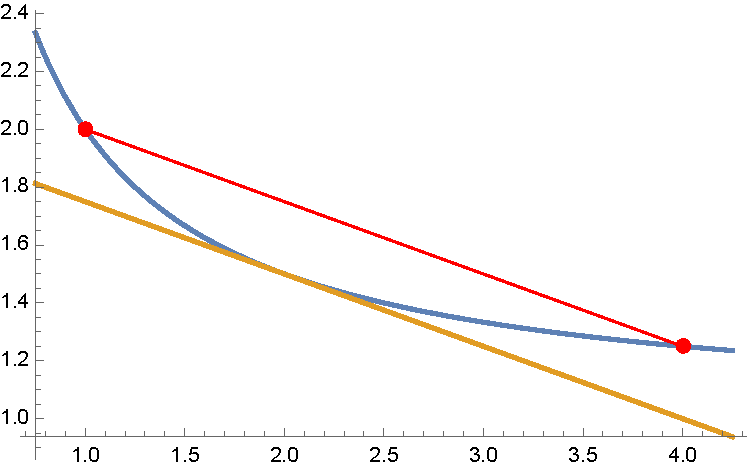
\includegraphics[width=0.4\textwidth]{Figures/mvt-graph.pdf}
        \caption{Tangent and secant lines for Example \ref{e:mvt}.}
        \label{f:mvt-graph}
    \end{figure}
\end{example}


\begin{theorem}\label{t:mvt-const-f}
    If \(f'(x) = 0\) over an interval, then f is constant over the interval.
\end{theorem}

We can use this to prove Euler's Formula!

\begin{theorem}\label{t:mvt-same-deriv}
    If \(f'(x) = g'(x)\) on an interval \(I\), then for all \(x\) in \(I\), \(f(x) = g(x) + C\), i.e. \(f\) and \(g\) differ by at most a constant.
\end{theorem}

This is the result we will end up using the most when we look at antiderivatives.

\section{L'Hospital's Rule}

Back to limits!

\begin{theorem}[L'Hospital's Rule]
    If \(\lim_{x \to a} \frac{f(x)}{g(x)}\) has the indeterminate form of either \(\frac{0}{0}\) or \(\frac{\infty}{\infty}\) then 
    \[\lim_{x \to a} \frac{f(x)}{g(x)} = \lim_{x \to a} \frac{f'(x)}{g'(x)}\]
    if the limit exists or is equal to \(\pm \infty\).
\end{theorem}
\begin{itemize}
    \item[{\faExclamationTriangle[solid]}] Note that this only applies to the \( \frac{0}{0}\) or \(\frac{\infty}{\infty}\) forms!
    \item  Main idea: functions look like their tangent lines when we zoom in close
\end{itemize}
\subsection{Basic Examples}
\begin{example}\label{e:lhr-basics}
    Evaluate each of the following limits using the most convenient and applicable method.
    \begin{enumerate}
        \item \(\displaystyle \lim_{x \to 3} \frac{x^{2} - 8x + 15}{x^{2} - 9} = \lim_{x \to 3} \frac{2x - 8}{2x} = -\frac{1}{3}\)
        \item \(\displaystyle \lim_{x \to -2} \frac{\ln(x+3)}{x + 2} = \lim_{x \to -2} \frac{\frac{1}{x+3}}{1} = 1\)
        \item May need to apply more than once: \(\displaystyle \lim_{x \to 0} \frac{e^{x} - x - 1}{x^{2}} = \lim_{x \to 0} \frac{e^{x} - 1}{2x} = \lim_{x \to 0} \frac{e^{x}}{2} = \frac{1}{2}\)
        \item \(\displaystyle \lim_{x \to \infty} \frac{x^{2} + x + 5}{3x^2 + 5x + 9} = \lim_{x \to \infty} \frac{2x + 1}{6x + 5} = \frac{2}{6} = \frac{1}{3}\) but we could have found this through dominant terms \faMeh
        \item \(\displaystyle \lim_{x \to \infty} \frac{x}{\sqrt{x^{2} + 1}} = \lim_{x \to \infty} \frac{1}{\frac{1}{2}(x^{2} + 1)^{-1/2}\cdot 2x} = \lim_{x \to \infty} \frac{\sqrt{x^{2} + 1}}{x} = \lim_{x \to \infty} \frac{x}{\sqrt{x^{2} + 1}}\) \faFrown \; unfortunately L'Hospital's Rule fails here. Use dominant terms instead.
    \end{enumerate}
\end{example}
\subsection{Indeterminate Products}
If the limit has the \(0 \cdot \infty\) form, then take:
\(\displaystyle \lim_{x \to a} f(x)g(x) = \lim_{x \to a} \frac{f(x)}{\frac{1}{g(x)}} \text{ or } \lim_{x \to a} \frac{g(x)}{\frac{1}{f(x)}}\)

Generally one of these will work and the other will not. May need trial-and-error. Usually you do not want to flip log functions.
\begin{example}
    Find \(\displaystyle \lim_{x \to 0^{+}} \sin x \ln x\).
    \begin{solution}
        \(\displaystyle \lim_{x \to 0^{+}} \sin x \ln x = \lim_{x \to 0^{+}} \frac{\ln x}{\csc x} = \lim_{x \to 0^{+}} \frac{\frac{1}{x}}{-\csc x \cot x} = - \lim_{x \to 0^{+}} \frac{\sin x \tan x}{x} = 0\)
    \end{solution}
\end{example}

\subsection{Indeterminate Differences}
This is the \(\infty - \infty\) form. What to do here just depends on the functions. Getting a common denominator if possible may help.

\begin{example}
    \(\displaystyle \lim_{x \to 0} \left(\csc x - \cot x\right) = 0\)
\end{example}

\subsection{Indeterminate Powers}
These are the \(0^{0}\), \(\infty^{0}\), and \(1^{\infty}\) forms. We generally proceed as follows:
\begin{align*}
    L       &= \lim_{x \to a} f(x)^{g(x)} \\
    \ln L   &= \ln \lim_{x \to a} f(x)^{g(x)}\\
            &= \lim_{x \to a} \ln f(x)^{g(x)}\\
            &= \lim_{x \to a} g(x)\ln f(x)
\end{align*}
This is guaranteed to be a \(0 \cdot \infty\) form, so evaluate the limit, then \(\displaystyle L = e^{\ln L} = e^{\lim_{x \to a} g(x)\ln f(x)}\) if the limit exists.

\begin{commentary}
    \textit{Usually} we will adopt the convention that \(0^0 = 1\). There's definitely a case for it! In a limit, though, we need to be a little more careful. Take the following two limits:
    \begin{align*}
        \lim_{x \to 0^+} \left(e^{-\frac{1}{x}}\right)^{x} &= e^{-1}\\
        \lim_{x \to 0^+} \left(e^{-\frac{1}{x}}\right)^{2x} &= e^{-2}
    \end{align*}
    Both of these have a \(0^0\) indeterminate form but different results. Most of the time, though, these forms will have a limit of 1.
\end{commentary}

\begin{example}
    Find each of the following limits.
    \begin{enumerate}
        \item \(\displaystyle \lim_{n \to \infty} \left(1 + \frac{1}{n}\right)^n = e\)
        \item \(\displaystyle \lim_{x \to 0^+} \ln (1 + \sin 3x)^{1/x} = 3\)
        \item \(\displaystyle \lim_{x \to \infty} (\cos x)^{1/x^2} = \frac{1}{\sqrt{e}}\)
    \end{enumerate}
\end{example}

\section{Graphing Functions Using Derivatives}
For tests, will break these down; do not have them do everything for one functions

\begin{example}\label{e:graph-polynomial}
    \(f(x) = x^3 - 3x^2 + 1\); \(f\) is increasing on \((-\infty, 0)\cup (2,\infty) \); decreasing on \((0,2)\); local maximum at \(x = 0\), local minimum at \(x=2\); concave up on \((1, \infty)\), concave down on \((\-\infty, 1)\), inflection point at \(x = 1\). See Figure \ref{f:graph-polynomial}.
    \begin{figure}[htbp]
        \centering
            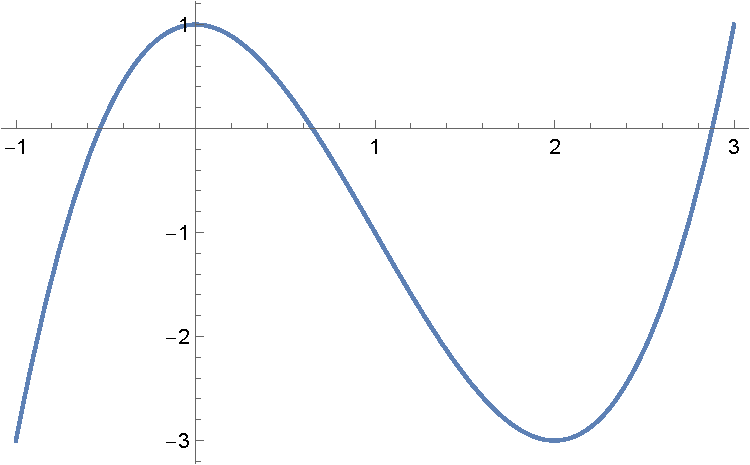
\includegraphics[width=0.4\textwidth]{Figures/graphing-polynomial.pdf}
        \caption{Graph for Example \ref{e:graph-polynomial}.}
        \label{f:graph-polynomial}
    \end{figure}
\end{example}

\begin{example}\label{e:graph-rational}
    \(\displaystyle f(x) = \frac{1}{x^2 - 1} \Rightarrow f'(x) = -\frac{2x}{(x^2 - 1)^2}, f''(x) = \frac{2 \left(3 x^2+1\right)}{\left(x^2-1\right)^3}\); Increasing on \((-\infty, -1)\cup (-1,0)\); decreasing on \((0,1)\cup(1,\infty)\); local maximum at \(x=0\) concave up on \((-\infty, -1) \cup (1, \infty)\), concave down on \((-1,1)\). No inflection point. See Figure \ref{f:graph-rational}.
    \begin{figure}[htbp]
        \centering
            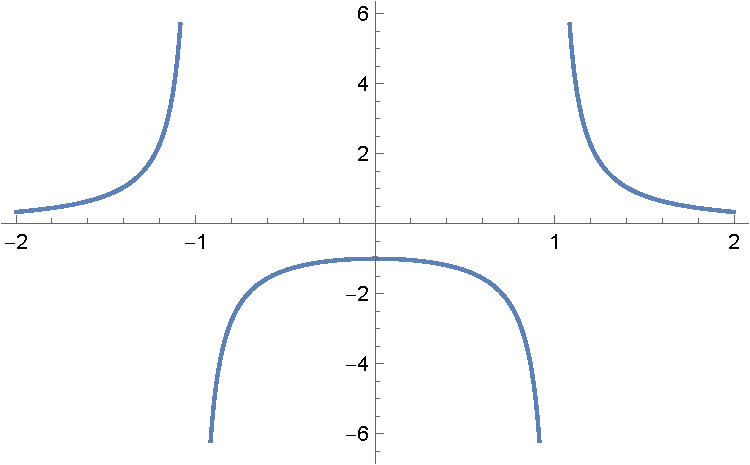
\includegraphics[width=0.4\textwidth]{Figures/graphing-rational.pdf}
        \caption{Graph for Example \ref{e:graph-rational}.}
        \label{f:graph-rational}
    \end{figure}
\end{example}

\begin{example}\label{e:graph-rational-oblique}
    \(\displaystyle f(x) = \frac{2 x^2-11 x+13}{x-4} =  2x - 3 +  \frac{1}{x-4} \Rightarrow f'(x) = 2-\frac{1}{(x-4)^2}, f''(x) = \frac{2}{(x-4)^3}\); Increasing on \(\left(-\infty, 4-\frac{1}{\sqrt{2}}\right)\cup \left(4+\frac{1}{\sqrt{2}}, \infty\right)\); decreasing on \(\left(4-\frac{1}{\sqrt{2}},4\right)\cup\left(4,4+\frac{1}{\sqrt{2}}\right)\); local maximum at \(x=4-\frac{1}{\sqrt{2}}\), local minimum at \(x=4+\frac{1}{\sqrt{2}}\)concave up on \(\left(4+\frac{1}{\sqrt{2}}, \infty\right)\), concave down on \(\left(-\infty,4-\frac{1}{\sqrt{2}}\right)\). No inflection point. See Figure \ref{f:graph-rational-oblique}.
    \begin{figure}[htbp]
        \centering
            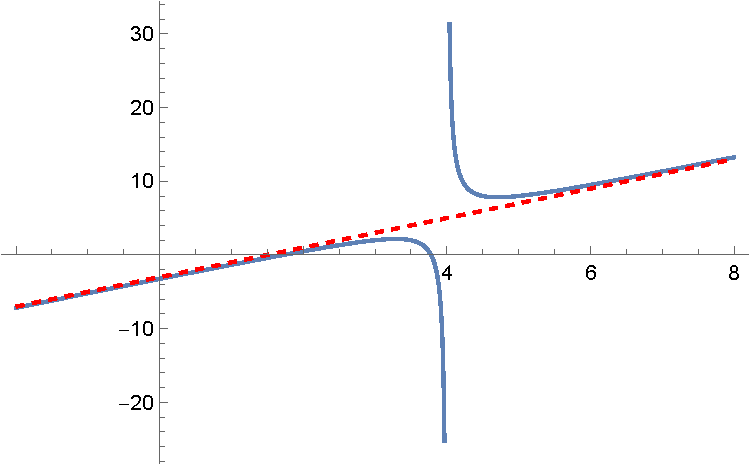
\includegraphics[width=0.4\textwidth]{Figures/graphing-rational-oblique.pdf}
        \caption{Graph for Example \ref{e:graph-rational-oblique}.}
        \label{f:graph-rational-oblique}
    \end{figure}
\end{example}


\begin{example}\label{e:graph-trig}
    \(f(x) = \cos^2 x - 2\sin x \Rightarrow f'(x) = -2 \cos x-2 \sin x \cos x, f''(x) = 2 \sin ^2 x + 2 \sin x -2 \cos ^2 x \); Increasing on \( \left(\frac{\pi}{2}, \frac{3\pi}{2}\right) \), decreasing on \( \left( 0, \frac{\pi}{2}\right) \cup \left( \frac{3\pi}{2}, 2\pi \right)\); local min at \(x = \pi/2\), local max at \(x = 3\pi /2\). Concave up on \(\left(0, \frac{5\pi}{6}\right)\), concave down on \(\left(\frac{5\pi}{6}, 2\pi\right)\). See Figure \ref{f:graph-trig}.
    \begin{figure}[htbp]
        \centering
            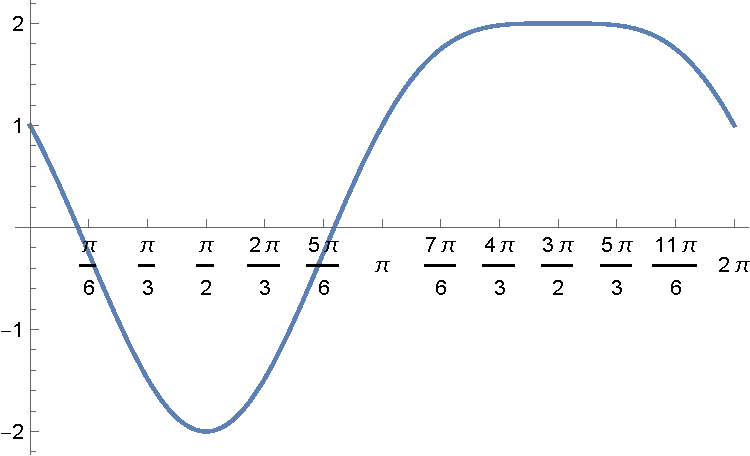
\includegraphics[width=0.4\textwidth]{Figures/graphing-trig.pdf}
        \caption{Graph for Example \ref{e:graph-trig}.}
        \label{f:graph-trig}
    \end{figure}
\end{example}

\section{Optimization Problems}
\begin{example}\label{optimize-core-problem}
    Find two real numbers whose difference is 100 and whose product is a minimum.
    \begin{solution}
        Let $x,y$ be the numbers; constraint is $x-y=100$ and we want to minimize $xy$. We can solve the constraining equation for either variable and sub in: $x = 100 + y \Rightarrow xy = (100+y)y = f(y) = 100y + y^{2}$. So we find the value of $y$ that minimizes $f(y)$. $f'(y) = 100 + 2y \Rightarrow f'(y) = 0$ when $y = -50 \Rightarrow x = 100 + (-50) = 50$. So the two numbers are 50 and $-50$.
    \end{solution}
\end{example}

\begin{example}\label{e:optimize-fence}
    A farmer wants to enclose a rectangular area with a fence with one side against a barn and subdivided into four rectangular areas using lengths of fence perpendicular to the barn wall. See Figure \ref{f:optimize-fence}.
    \begin{figure}[htbp]
        \centering
            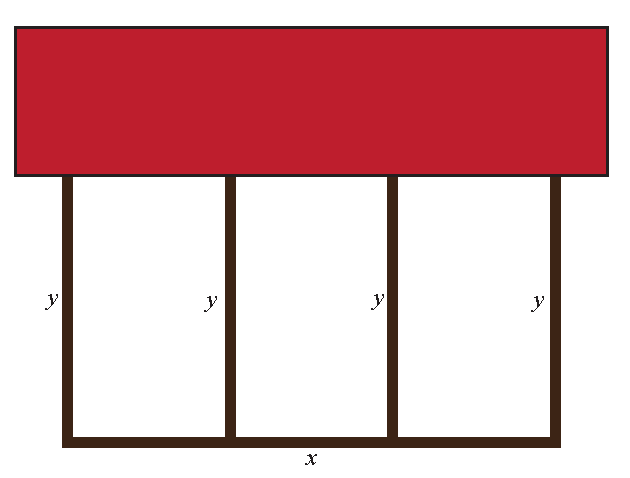
\includegraphics[width=0.3\textwidth]{Figures/opt-barn.pdf}
        \caption{Area setup for Example \ref{e:optimize-fence}.}
        \label{f:optimize-fence}
    \end{figure}
    \begin{enumerate}%[label=\bfseries\alph*.]
        \item If 200 m of fencing is available, what dimensions will maximize the enclosed area?
        \begin{solution}
            Want to maximize \(A(x,y) = xy\) subject to \(x + 4y = 200 \Rightarrow x = 200-4y\). Thus \(A(x) = (200-4y)y = 200y - 4y^{2}\); now \(A'(y) = 200 - 8y \Rightarrow A'(y) = 0\) when \(y = 25\). Note that \(A''(y) = -8 \Rightarrow A''(25) = 8 >0\) so this produces a maximum. So \(x = 200-4(25) = 100\) and the dimensions are 100 feet by 25 feet.
        \end{solution}
        \item Now suppose that the farmer wants to enclose an area of exactly 2000 square meters. What dimensions will minimize the fencing used?
        \begin{solution}
            Now we want to minimize \(f(x,y) = x + 4y = 200\) subject to \(xy = 2000 \Rightarrow y = \frac{2000}{x}\). So \(f(x) = x + \frac{8000}{x} \Rightarrow f'(x) = 1 - \frac{8000}{x^{2}} \Rightarrow A'(x) = 0\) when \(x^{2} = 8000 \Rightarrow x = 20\sqrt{20}\). Note that we omit the negative solution as we are dealing with lengths. Also \(f''(x) = \frac{16000}{x^{3}} \Rightarrow f''(20\sqrt{20}) = \frac{16000}{(20\sqrt{20})^{3}}> 0\) so we have a minimum at the critical point. So \(y = 10\sqrt{5}\) and the dimensions are \(40\sqrt{5}\) feet by \(10\sqrt{5}\) feet.
        \end{solution}
    \end{enumerate}
\end{example}

\begin{example}\label{e:optimize-dog-snow}
    A dog is sitting in a snow-covered yard 10 meters from a sidewalk. The sidewalk is clear of snow and dry. The dog wants to run to their friend that is standing 20 meters from the point on the sidewalk closest to the dog. The dog can run 4 m/s in the snow and 8 m/s along the sidewalk. Where should the dog run to to minimize the time it takes to get to his friend?
    \begin{solution}
        Let \(x\) be the distance from the point on the sidewalk closest to the dog to the point he wants to run to. Then:
        \begin{align*}
            t(x) &= \frac{\sqrt{x^{2} + 100}}{4} + \frac{20-x}{8}\\
            t'(x) &= \frac{x}{4 \sqrt{x^2+100}}-\frac{1}{8}
        \end{align*}
        Set \(t'(x) = 0\) and solve to get \(x = \frac{10}{\sqrt{3}}\). But here we have a closed interval of values to consider, \([0, 20]\). So we calculate \(t(x)\) at the critical point and endpoints:
        \begin{align*}
            t(0) &= 5\\
            t(20) &= \frac{5\sqrt{5}}{2} \approx 5.59\\
            t\left(\frac{10}{\sqrt{3}}\right) &= \frac{5}{4} \left(\sqrt{3}+2\right) \approx 4.67
        \end{align*}
    So the dog should run to the point on the sidewalk that is \(\frac{10}{\sqrt{3}}\) m from the point on the sidewalk closest to him. \faSmile \ Note that this saves about a third of a second from running straight to their friend, and about a second versus running straight to the road. \faMeh
    \end{solution}
\end{example}


\section{Antiderivatives}

\begin{definition}\label{d:antiderivative}
    We say that \(F\) is an \textbf{antiderivative} of \(f\) on an interval \(I\) if \(F'(x) = f(x)\) for all \(x\) in \(I\).
\end{definition}
\begin{itemize}
    \item Note that we say "an" antiderivative not "the" antiderivative
\end{itemize}
\begin{example}
    Say \(f(x) = 3x^{2}\). Then \(g(x) = x^{3}\) is an antiderivative of \(f\) because \(g'(x) = 3x^{2} = f(x)\). But for \(h(x) = x^{3} + 10\), \(h'(x) = 3x^{2}\) so \(h\) is also an antiderivative of \(f\). In fact any function of the form \(F(x) = x^{3} + C\), where \(C\) is any real number, has \(F'(x) = 3x^{2}\) so these are all antiderivatives of \(f\). We call this the \textbf{most general antiderivative} of \(f\).

    Are there any others that are different? Nope! By Theorem \ref{t:mvt-same-deriv} we know that if two functions have the same derivative (so they are both antiderivatives of the same function), they can differ by at most a constant. So this is it! \faSmile
\end{example}


\begin{table}[htbp]
    \centering\begin{tabular}{Sl Sl}
        \textbf{Function} & \textbf{Particular Antiderivative} \\ \hline
        \(f(x) \pm g(x)\)   & \(F(x) \pm G(x)\)\\
        \(cf(x)\)   & \(cF(x)\)\\
        \(x^{n}, n \neq -1\)    & \(\dfrac{x^{n+1}}{n+1}\)\\
        \(e^x\) & \(e^x\)\\
        \(b^x\) & \(\dfrac{b^x}{\ln b}\)\\
        \(\frac{1}{x}\) & \(\ln |x|\)\\
        \(\sin x\) & \(-\cos x\)\\
        \(\cos x\) & \(\sin x\)\\
        \(\sec^2 x\) & \(\tan x\)\\
        \(\sec x \tan x\) & \(\sec x\)\\
        \(\dfrac{1}{1 + x^2}\) & \(\tan^{-1} x\)\\
        \(\dfrac{1}{\sqrt{1 - x^2}}\) & \(\sin^{-1} x\)\\
        \(\dfrac{1}{x\sqrt{x^2 - 1}}\) & \(\sec^{-1} x\)\\ \hline
    \end{tabular}
    \caption{Antiderivative rules.}
    \label{tb:antiderivative}
\end{table}

\begin{example}
    Find the general antiderivative of each function.
    \begin{enumerate}
        \item \(f(x) = x^3-4 x^2-5 x+7 \Rightarrow F(x) = \frac{x^4}{4}-\frac{4 x^3}{3}-\frac{5 x^2}{2}+7 x + C \)
        \item \(f(x) = \sin x - 4\cos x + \sec^2 x \Rightarrow F(x) = -\cos x - 4\sin x + \tan x + C\)
        \item \(f(x) = (x+1)(x-4) = x^2 - 3x - 4 \Rightarrow F(x) = \frac{x^3}{3} - \frac{3}{2}x - 4x + C\)
        \item \(f(x) = \dfrac{x - x^2}{x^3} = x^{-2} + x^{-1}\Rightarrow F(x) = -x^{-1} + \ln |x| + C \)
     \end{enumerate}
\end{example}

So why would we even want these? We will see soon!

\subsection{Initial Value Problems}

Given the derivative of a function and one value of the function, we can find a unique solution! One way to interpret the derivative is that it tells what direction the graph goes in. So if we know where the graph "starts" and what direction it must go in from there, we know the function.

This can be extended to the problem where we know the second derivative and vales of the first derivative and the function.

\begin{example}\label{e:antiderivative-ivp}
    \begin{enumerate}
        \item \(f'(x) = 4x^3 + 6x, f(1) = -5 \Rightarrow f(x) = x^4+3 x^2-9\)
        \item \(f'(x) = e^x - 3\cos x, f(0) = 2 \Rightarrow f(x) = e^x-3 \sin x + 1 \)
        \item \(f''(x) = 12x^2 + 4e^{x}, f'(0) = 3, f(0) = -1 \Rightarrow f(x) = x^4-x+4 e^x-5\)
        \item \(f''(x) = 24x^3 - 6x, f(0) = -2, f(1) = 3 \Rightarrow f(x) = \frac{6 x^5}{5}-x^3+\frac{24 x}{5}-2\)
    \end{enumerate}
\end{example}

\newpage\thispagestyle{firstofchapter}
\chapter{Areas and Integrals}
\section{The Area Problem}
\begin{commentary}
    I generally do not do much with this just go over the basic idea that we do this by pretending the function is constant over a little interval then take a limit
\end{commentary}
\subsection{Sigma Notation}
Before getting into the area problem, we need to look at sigma notation first
\[\sum_{i=m}^{n} a_{i} = a_{m} + a_{m+1} + a_{m+2} + \cdots + a_{n}\]

This gives us a compact way to write a long sum.

\begin{example}\label{e:sigma-basic}
    \begin{enumerate}
        \item \(\displaystyle \sum_{i=1}^{6} 2i = 2 + 4 + 6 + 8 + 10 + 12 = 42\)
        \item \(\displaystyle \sum_{k=1}^{4} \frac{k}{k + 1} = \frac{1}{2} + \frac{2}{3} + \frac{3}{4} + \frac{4}{5} = \frac{163}{60}\)
    \end{enumerate}
\end{example}
Note that this is not unique; the last sum above can be written as \(\displaystyle \sum_{k=0}^{3} \frac{k + 1}{k + 2} \text{ or } \sum_{k=2}^{3} \frac{k - 1}{k}\) by shifting indices; of course letter used for index does not matter either.

We also have some nice properties and formulas we can use:

\begin{itemize}
    \item \(\displaystyle \sum_{i=m}^{n} a_i \pm \sum_{i=m}^{n} b_i = \sum_{i=m}^{n} (a_i \pm b_i)\) Note that this does not work for multiplication nor does it work for division
    \item \(\displaystyle c \sum_{i=m}^{n} a_i = \sum_{i=m}^{n} c a_i\)
    \item \(\displaystyle \sum_{i=1}^{n} 1 = n\)
    \item \(\displaystyle \sum_{i=1}^{n} i = \frac{n(n+1)}{2}\)
    \item \(\displaystyle \sum_{i=1}^{n} i^2 = \frac{n(n+1)(2n+1)}{6}\)
    \item \(\displaystyle \sum_{i=1}^{n} i^3 = \left(\frac{n(n+1)}{2}\right)^2\)
    
\end{itemize}

\subsection{Area Under A Curve}

Now the main problem: find the area bounded by the graph of a continuous function over a closed interval \(I = [a,b]\)!

\begin{itemize}
    \item Divide \(I\) into \(n\) equally spaced subintervals with width \(\Delta x = \frac{b-a}{n}\)
    \item Let \(x_0 = a, x_1 = x_0 + \Delta x, x_2 = x_1 + \Delta x, \ldots, x_n = b\)
    \begin{itemize}
        \item So \(i\)\textsuperscript{th} subinterval is \([x_{i-1}, x_i]\)
    \end{itemize}
    \item Pick sample point in each subinterval \(x_{i}^{*}\) and calculate \(f(x_{i}^{*})\)
    \item Now make a rectangle in each subinterval with width \(\Delta x \) and height \(f(x_{i}^{*})\)
    \item Sum areas of rectangles to get \(\displaystyle \sum_{i=1}^{n} f(x_{i}^{*}) \Delta x\), the \textbf{Riemann Sum}
    \item Now as we do in Calculus use a limit to make this what we want and get...
\end{itemize}
\[A = \lim_{n\to\infty} \sum_{i=1}^{n} f(x_{i}^{*}) \Delta x \]
\begin{center}
    \Huge \faMeh
\end{center}

This is hard to do even with nice functions. Fortunately there may be a much easier way! \faSmile

\section{The Definite Integral}
\begin{definition}\label{d:definite-integral}
    The \textbf{definite integral} from \(a\) to \(b\) of \(f\) with respect to \(x\) is
    \[\int_a^b f(x) \, dx = \lim_{n\to\infty} \sum_{i=1}^{n} f(x_{i}^{*}) \Delta x\]
\end{definition}

For now we will just interpret this as the net area (area above \(-\) area below) bounded by the graph of \(f\) and the \(x\)-axis

\begin{example}
    Evaluate each integral in terms of area bounded by the graph.
    \begin{enumerate}
        \item \(\int_{-4}^{4} (3x + 2) \, dx = 16\)
        \item \(\int_{-3}^{3} \sqrt{9-x^{2}} \, dx = \frac{9\pi}{2}\)
    \end{enumerate}
\end{example}

\subsection{Properties of the Definite Integral}
We will use these all at some point!

\begin{itemize}
    \item \(\displaystyle \int_a^a f(x) \, dx = 0\) \faMeh
    \item \(\displaystyle \int_a^b f(x) \, dx = - \int_b^a f(x) \, dx\)
    \item \(\displaystyle \int_a^b (f(x)  \pm g(x)) \, dx = \int_a^b f(x) \, dx \pm \int_a^b g(x) \, dx\)
    \item \(\displaystyle \int_a^b c f(x) \, dx = c \int_a^b f(x) \, dx\)
    \item \(\displaystyle \int_a^b f(x) \, dx = \int_a^c f(x) \, dx + \int_c^b f(x) \, dx\)
    \item \(\displaystyle \int_a^b c \, dx = c(b-a)\)
    \item If \(f(x) \leq g(x)\) on \([a,b]\) then \(\displaystyle \int_a^b f(x) \, dx \leq \int_a^b g(x) \, dx\)
    \item If \(m \leq f(x) \leq M\) on \([a,b]\) then \(\displaystyle m(b-a) \leq \int_a^b f(x) \, dx \leq M(b-a)\)
\end{itemize}
\section{The Fundamental Theorem of Calculus}
\begin{theorem}[Fundamental Theorem of Calculus, Part I]\label{t:FTOC-I}
    If \(f\) is continuous on \([a,b]\), then the function
    \[g(x) = \int_a^x f(t) \, dt\]
    is continuous on \([a,b]\), differentiable on \((a,b)\), and \(g'(x) = f(x)\).
\end{theorem}

This means that this integral function \(g\) is an antiderivative of \(f\)!

\begin{example}\label{e:ftoc-ptI}
    \begin{enumerate}
        \item \(\displaystyle \frac{d}{dx} \int_2^x \sin t \, dt = \sin x\)
        \item \(\displaystyle \frac{d}{dx} \int_x^4 (t^2 + 1) \, dt = -(x^2 + 1)\)
        \item Using the Chain Rule: \(\displaystyle \frac{d}{dx} \int_{1}^{e^x} \frac{1}{1 + t} \, dt = \frac{e^x}{1 + e^x}\)
    \end{enumerate}
\end{example}

\begin{theorem}[Fundamental Theorem of Calculus, Part II]\label{t:FTOC-II}
    If \(f\) is continuous on \([a,b]\) and \(F\) is any antiderivative of \(f\), then
    \[\int_a^b f(x) \, dx = F(x)\Big|_a^b = F(b) - F(a).\]
\end{theorem}

\begin{example}\label{e:ftoc-ptII}
    \begin{enumerate}
        \item \(\displaystyle \int_{-1}^2 \left(x^2-3 x+1\right) \, dx = \frac{3}{2}\)
        \item \(\displaystyle \int_{-\pi/4}^{\pi /2} 3 \sin (x) \, dx = \frac{3}{\sqrt{2}}\)
        \item \(\displaystyle \int_0^1 (x+3) (x-5) \, dx = -\frac{47}{3}\)
    \end{enumerate}
\end{example}

\section{More With Definite Integrals}

\subsection{Odd and Even Functions}
\begin{theorem}\label{t:odd-even-integrals}
    If \(f\) is even on \([a,b]\) then
    \[\int_{-a}^{a} f(x) \, dx = 2\int_{0}^{a} f(x) \, dx\]
    If \(f\) is odd on \([a,b]\) then
    \[\int_{-a}^{a} f(x) \, dx = 0\]
\end{theorem}

\begin{example}
    \begin{enumerate}
        \item \(\displaystyle \int_{-3}^{3} x^4 \tan x \, dx = 0\) \faSmile
        \item \(\displaystyle \int_{-1}^{1} \left(x^{19} + x^{13 }+ x^{7} + x^2\right) \, dx = \int_{-1}^{1} x^2 \, dx = \frac{2}{3}\)
    \end{enumerate}
\end{example}

\subsection{Average Value of a Function}
\begin{theorem}\label{t:avg-value-of-f}
    If \(f\) is continuous on \([a,b]\) then the average value of \(f\) over \([a,b]\) Is
    \[\bar{f} = \frac{1}{b-a} \int_a^b f(x) \, dx\]
\end{theorem}

\begin{example}
    Find the average value of \(f(x) = x^3 - x\) over the interval \([-3, 1] \).
    \begin{solution}
        \[\bar{f} = \frac{1}{4} \int_{-3}^{1} \left(x^3 - x\right) \, dx = 4\]
    \end{solution}
\end{example}

\subsection{Total Change}
Another way to write FToC Part II is to say
\[\int_a^b f'(x) dx = f(b) - f(a)\]
One way to interpret this is to keep in mind that for small \(h\), \(f(x+\Delta x) - f(x) \approx f'(x)\Delta x\); so when we divide \([a,b]\) in small subintervals of width \(\Delta x\), \textit{the total change in \(f\) over \([a,b]\) is the same as the sum of the little changes along the way}. In other words,
\[\int_a^b f'(x) dx \approx \sum f'(x) \Delta x \approx \sum \left(f(x+\Delta x) - f(x)\right)= f(b) - f(a)\]
\section{The Substitution Rule}

\subsection{Indefinite Integrals}

\begin{theorem}[Substitution Rule for Indefinite Integrals]\label{t:sub-rule-indef-int}
    \[\int f(g(x))g'(x)\, dx = \int f(u) \, du\]
    with the substitution \(u=g(x) \Rightarrow du = g'(x) \, dx\).
\end{theorem}

\begin{example}
    \begin{enumerate}
        \item \(\displaystyle \int 2 x \sqrt{x^2+1} \, dx = \frac{2}{3} \left(x^2+1\right)^{3/2} + C\)
        \item \(\displaystyle \int \frac{\sin (x)}{\cos ^3(x)} \, dx = \frac{\sec ^2 x}{2} + C\)
        \item \(\displaystyle \int x \sqrt{x+2} \, dx = \frac{2}{15} (x+2)^{3/2} (3 x-4) + C\)
        \item \(\displaystyle \int \frac{\log ^3(x)}{x} \, dx = \frac{\log ^4(x)}{4} + C\)
    \end{enumerate}
\end{example}

\subsection{Definite Integrals}

\begin{theorem}[Substitution Rule for Definite Integrals]\label{t:sub-rule-def-int}
    \[\int_{a}^{b} f(g(x))g'(x)\, dx = \int_{g(a)}^{g(b)} f(u) \, du\]
    with the substitution \(u=g(x) \Rightarrow du = g'(x) \, dx\).
\end{theorem}

\begin{example}
    \begin{enumerate}
        \item \(\displaystyle \int_0^1 2 x \left(3 x^2+1\right)^2 \, dx = 7\)
        \item \(\displaystyle \int_{e^2}^{e^5} \frac{1}{x \ln^2(x)} \, dx = \frac{3}{10}\)
        \item \(\displaystyle \int_0^2 \frac{x}{(x+2)^2} \, dx = -\frac{1}{2} + \ln 2\)
        \item \(\displaystyle \int_0^{\frac{\pi }{4}} \sin ^2(x) \, dx = \frac{\pi -2}{8}\)
        \item \(\displaystyle \int_0^1 \frac{1}{x^2+2 x+1} \, dx  = \frac{1}{2}\)
    \end{enumerate}
\end{example}

\subsection{Tangent and Secant Integrals}
\begin{theorem}
    The following both follow from substitution.
    \begin{enumerate}
        \item \(\displaystyle \int \tan x \, dx = \ln |\sec x| + C\)
        \item \(\displaystyle \int \sec x \, dx = \ln |\sec x + \tan x| + C\)
    \end{enumerate}
\end{theorem}


\newpage
\part{Calculus II}
\thispagestyle{firstofchapter}
\chapter{Applications of Integrals}
\section{Areas Between Curves}
\setcounter{figure}{0}

\begin{itemize}
    \item $\displaystyle A = \int_{a}^{b} \left| f(x) - g(x)\right|\, dx$
    \item Always look for where $f(x) = g(x)$ first, break up integral as needed
\end{itemize}

\begin{example}
    \label{e:arealineparabola} Find the area between the graphs of $f(x) = x^{2}$ and $g(x) = x + 2$, \(-1 \leq x \leq 2.\).
    \begin{figure}[htbp]
        \centering
            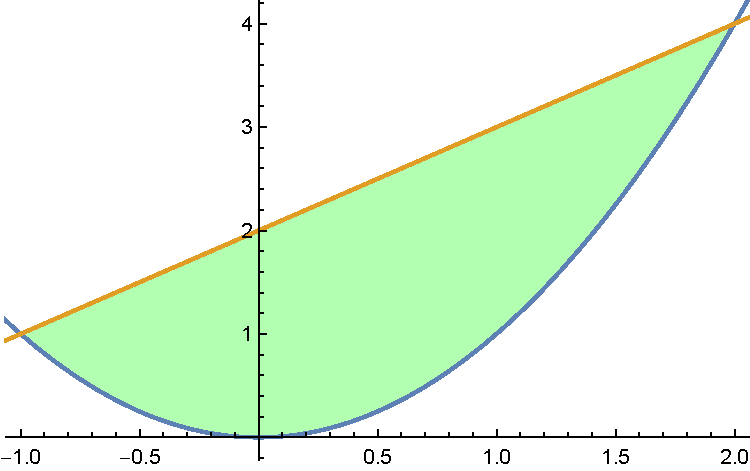
\includegraphics[width=0.4\textwidth]{Figures/arealineparabola.pdf}
        \caption{Region for Example \ref{e:arealineparabola}.}
        \label{f:arealineparabola}
    \end{figure}

    \begin{solution}
        $x^{2} = x + 2 \Rightarrow x = -1,2$ so the area is
        \[\int_{-1}^{2} \left( x + 2 - x^{2} \right)\, dx = \frac{9}{2}\]
    \end{solution}
\end{example}

\begin{example}
    \label{e:areasqrt} Find the area between the graphs of $f(x) = \sqrt{x}$ and $g(x) = x$, $0 \leq x \leq 2$.
    \begin{figure}[htbp]
        \centering
            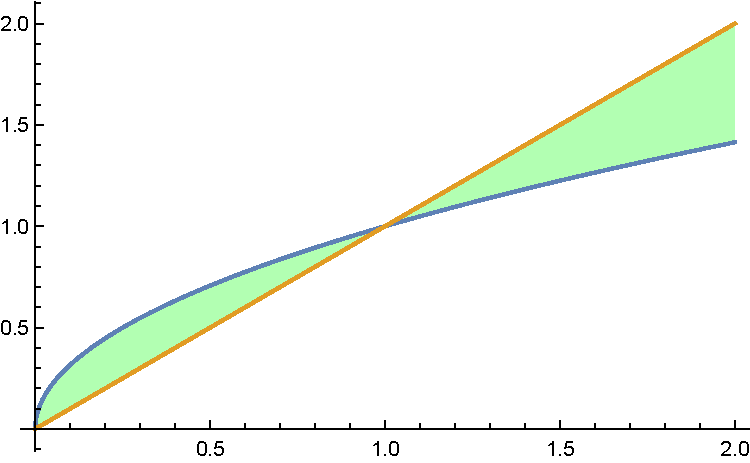
\includegraphics[width=0.4\textwidth]{Figures/areasqrt.pdf}
        \caption{Region for Example \ref{e:areasqrt}.}
        \label{f:areasqrt}
    \end{figure}   
    
    \begin{solution}
        $\sqrt{x} = x \Rightarrow x = 0, 1$ so the area is
        \[\int_{0}^{1} \left( \sqrt{x} - x \right)\, dx + \int_{1}^{2} \left( x - \sqrt{x} \right) \, dx = \frac{1}{3}\left( 7 - 4\sqrt{2} \right)\]
    \end{solution}
\end{example}

\begin{example}
    \label{e:areatrig2xident} Find the area between the graphs of $f(x) = \cos x$ and $g(x) = \sin 2x$, $0 \leq x \leq \frac{\pi}{2}$.
    \begin{figure}[htbp]
        \centering
            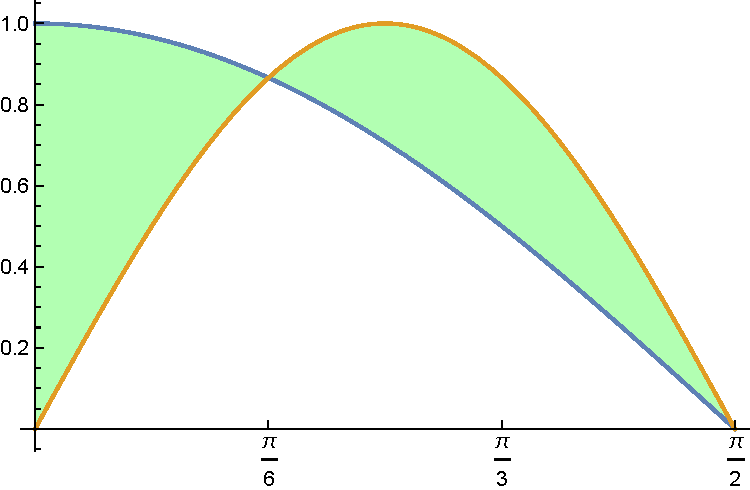
\includegraphics[width=0.4\textwidth]{Figures/areatrig2xident.pdf}
        \caption{Region for Example \ref{e:areatrig2xident}.}
        \label{f:areatrig2xident}
    \end{figure}
    
    \begin{solution}
        $\cos x = \sin 2x \Rightarrow \cos x = 2\sin x \cos x \Rightarrow x = \frac{\pi}{6}, \frac{\pi}{2}$, so the area is
        \[\int_{0}^{\pi /6} \left( \cos x - \sin 2x \right)\, dx + \int_{\pi/6}^{\pi/2} \left( \sin 2x - \cos x \right)\, dx = \frac{1}{2}\]
    \end{solution}
\end{example}

\begin{example}
    \label{e:areawrty} Find the area between $x = -\sin y$ and $x = \cos y$, $-\pi /4 \leq y \leq 3\pi/4$.
    \begin{figure}[htbp]
        \centering
            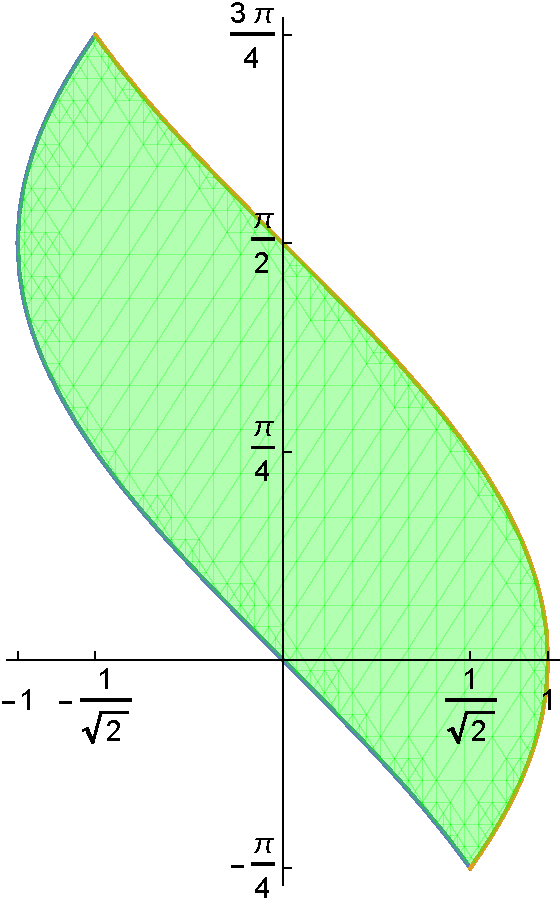
\includegraphics[width=0.2\textwidth]{Figures/areawrty.pdf}
        \caption{Region for Example \ref{e:areawrty}.}
        \label{f:areawrty}
    \end{figure}
    
    \begin{solution}
        Note that these are the two points of intersection near $y=0$; so the area is
        \[\int_{-\pi/4}^{3\pi/4} \left( \cos y + \sin y \right)\, dy = 2\sqrt{2}\] 
    \end{solution}  
\end{example}

\section{Volumes by Disks or Washers}
\setcounter{figure}{0}

    In general if we know the cross-sectional area of a solid $A(x)$ we can find the volume by taking
    \[V = \int_{a}^{b} A(x) \, dx\]
    If the solid was made by rotating the graph of $y = f(x), a\leq x \leq b$, the cross-sectional area is $A(x) = \pi [f(x)]^{2}$ so the volume is
    \[V = \pi \int_{a}^{b} [f(x)]^{2} \, dx\]
    If we want to rotate the region between $f(x)$ and $g(x)$, assuming $|f(x)| \geq |g(x)|$ on $[a,b]$, the volume is
    \[V = \pi \int_{a}^{b} \left[ (f(x))^{2} - (g(x))^{2} \right]\, dx\]

\begin{example}
    \label{e:volcsparabola} Find the volume of the solid made by revolving the given region $R$ about the given axis: \\$R = \left\{ (x,y) \ | \ 0 \leq x \leq 1, 0 \leq y \leq x^{2} \right\}$ about $y = 0$
    
    \begin{figure}[htbp]
    \centering
        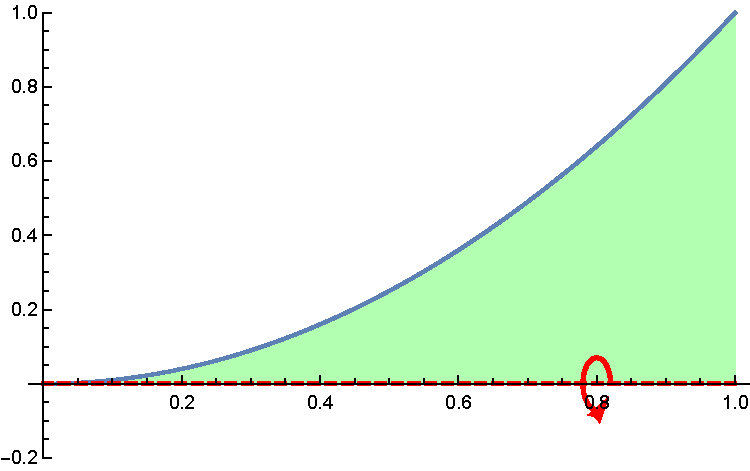
\includegraphics[width=0.4\textwidth]{Figures/volcsparabola.pdf}
    \caption{Region for Example \ref{e:volcsparabola}.}
    \label{f:volcsparabola}
    \end{figure}    
    
    \begin{solution}
        \[V = \pi \int_{0}^{1} (x^{2})^{2} x \, dx = \frac{\pi}{5}\]
    \end{solution}
\end{example}


\begin{example}
    \label{e:volcstrigshift} Find the volume of the solid made by revolving the given region $R$ about the given axis: \\$R = \left\{ (x,y) \ | \ 0 \leq x \leq \pi/2, 1 \leq y \leq 1 + \cos x \right\}$ about $y = 1$.
    
    \begin{figure}[htbp]
        \centering
            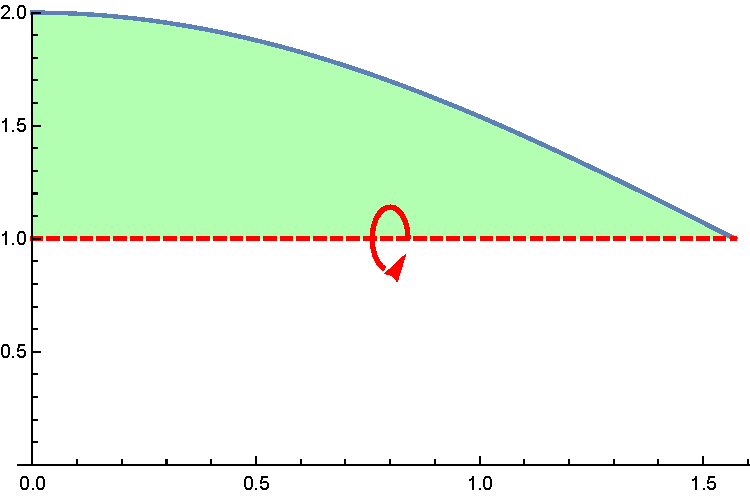
\includegraphics[width=0.4\textwidth]{Figures/volcstrigshift.pdf}
        \caption{Region for Example \ref{e:volcstrigshift}.}
        \label{f:volcstrigshift}
    \end{figure}

    \begin{solution}
        The half-angle identity $\cos^{2} x = \frac{1}{2}\left( 1 + \cos 2x \right)$ is needed here:
        \[V = \pi \int_{0}^{\pi/2} \cos^{2} x \, dx = \pi \int_{0}^{\pi/2} \frac{1}{2}\left( 1 + \cos 2x \right) x \, dx = \frac{\pi^{2}}{4}\]
    \end{solution}
\end{example}

\begin{example}
    \label{e:vol-disk-sqrt} Find the volume of the solid made by revolving the given region $R$ about the given axis: \\$R = \left\{ (x,y) \ | \ 0 \leq x \leq 16, 4 \leq y \leq 4 - \sqrt{x}  \right\}$ about $y = 4$.

    \begin{figure}[htbp]
        \centering
            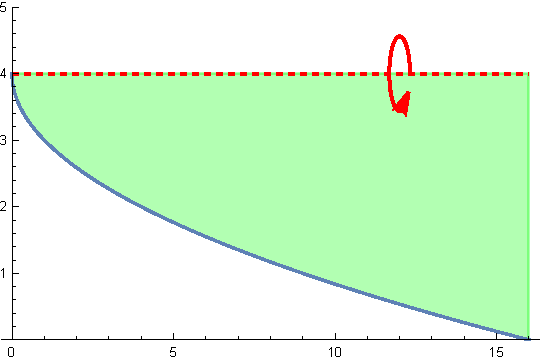
\includegraphics[width=0.4\textwidth]{Figures/vol-Disc-SQrt.pdf}
        \caption{Region for Example \ref{e:vol-disk-sqrt}.}
        \label{f:vol-disk-sqrt}
    \end{figure}

    \begin{solution}
        The distance from the axis of rotation to the boundary of the figure is \(4 - (4 - \sqrt{x}) = \sqrt{x}\) \faSmile \; so the volume is
        \[ V = \pi \int_{0}^{16} (\sqrt{x})^{2} \, dx = \pi \int_{0}^{16} x \, dx = 128\pi \]

    \end{solution}

\end{example}

\begin{example}
    \label{e:volscsqrtwrty} Find the volume of the solid made by revolving the given region $R$ about the given axis: \\$R = \left\{ (x,y) \ | \ 0 \leq x \leq y^{2}, 0 \leq y \leq 1 \right\}$ about $x = -1$
    
    \begin{figure}[htbp]
        \centering
            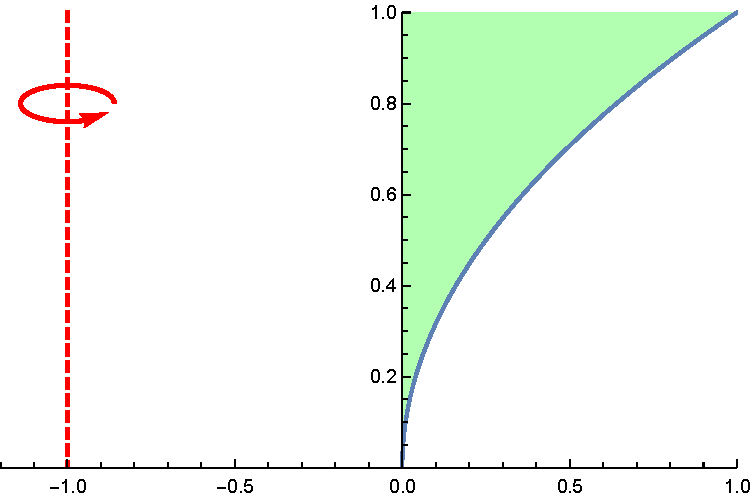
\includegraphics[width=0.4\textwidth]{Figures/volscsqrtwrty.pdf}
        \caption{Region for Example \ref{e:volscsqrtwrty}.}
        \label{f:volscsqrtwrty}
    \end{figure}
    
    \begin{solution}
        \[V = \pi \int_{0}^{1} \left[ \left( y^{2} + 1 \right)^{2} - 1 \right]\, dy = \pi \int_{0}^{1} \left( y^{4} + 2y^{2} \right)\, dy = \frac{13\pi}{15}\]
    \end{solution}
\end{example}
    
\begin{itemize}
    \item Above examples have consistent radii
    \item If $y = f(x)$ is not one-to-one and axis vertical? \faFrown
    \item Maybe Shell Method! \faSmile
\end{itemize}

\section{Volumes by Shells}
\setcounter{figure}{0}

\begin{itemize}
    \item Use cylindrical shells to approximate area
    \item Inner radius $r_{1}$, outer radius $r_{2}$, height $h$; makes volume of shell
    \[V_{\text{shell}} = \pi (r_{2}^{2} - r_{1}^{2}) h = \pi (r_{2}+r_{1})(r_{2} - r_{1})h = 2\pi \left( \frac{r_{2} + r_{1}}{2} \right)(r_{2} - r_{1})h  \]
    \item Note that $\frac{r_{2} + r_{1}}{2}$ is the average of the radii, so we let $x = \frac{r_{2} + r_{1}}{2}$; $r_{2} - r_{1}$ is the thickness of the shell, so let $\Delta x = r_{2} - r_{1}$; $h$ is the height of shell, so take $h = f(x)$. This makes the volume of the shell
    \[V_{\text{shell}} = 2 \pi x f(x) \Delta x  \]
    \item Add them up, take $\Delta x \to 0$ to get
    \[V = 2\pi \int_{a}^{b} x f(x) \, dx  \]
    \item More generally
    \[V = 2\pi \int_{a}^{b} \text{(Distance from axis to shell)(height of shell)}\, dx    \]
\end{itemize}

\begin{example}
    \label{e:volshparabola}$R = \left\{ (x,y) \ | \ 0 \leq x \leq 4, 0 \leq y \leq 4-\left( x - 2 \right)^{2} \right\}$ about the $y$-axis
    \begin{figure}[htbp]
        \centering
            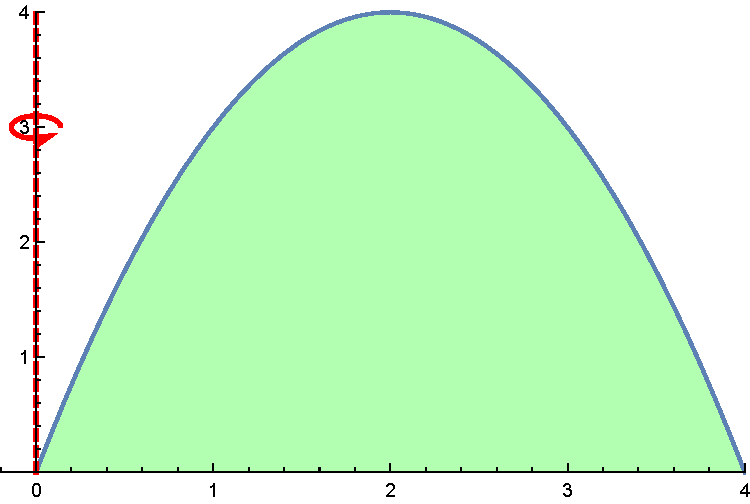
\includegraphics[width=0.4\textwidth]{Figures/volshparabola.pdf}
        \caption{Region for Example \ref{e:volshparabola}.}
        \label{f:volshparabola}
    \end{figure}
    
    \begin{solution}
        \[V = 2\pi \int_{0}^{4} x\left( 4-\left( x - 2 \right)^{2} \right) \, dx = 2\pi \int_{0}^{4} \left( 4x^{2} - x^{3} \right)\, dx = \frac{128\pi}{3}\]
    \end{solution}
\end{example}

\begin{example}
    \label{e:volshrecip}$R = \left\{ (x,y) \ | \ 1 \leq x \leq 2, 0 \leq y \leq \frac{1}{x} \right\}$ about $x = -2$
    \begin{figure}[htbp]
        \centering
            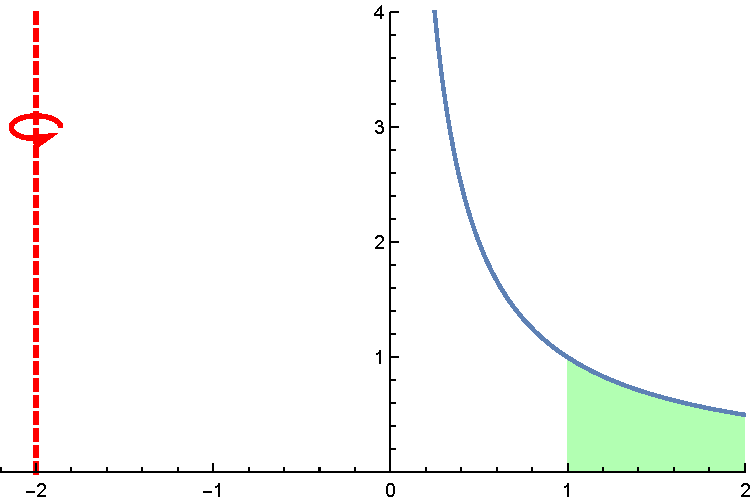
\includegraphics[width=0.4\textwidth]{Figures/volshrecip.pdf}
        \caption{Region for Example \ref{e:volshrecip}.}
        \label{f:volshrecip}
    \end{figure}
    
    \begin{solution}
        \[V = 2\pi\int_{1}^{2}\left( x+ 2 \right)\cdot\frac{1}{x}\, dx = 2\pi\int_{1}^{2} \left( 1 + \frac{2}{x} \right)\, dx = 2\pi \left( 1 + 2 \ln 2 \right)\]
    \end{solution}
\end{example}

\begin{example}
    \label{e:volshexp}$R = \left\{ (x,y) \ | \ 0 \leq x \leq 1, 0 \leq y \leq e^{-x^{2}} \right\}$ about $y$-axis
    \begin{figure}[htbp]
        \centering
            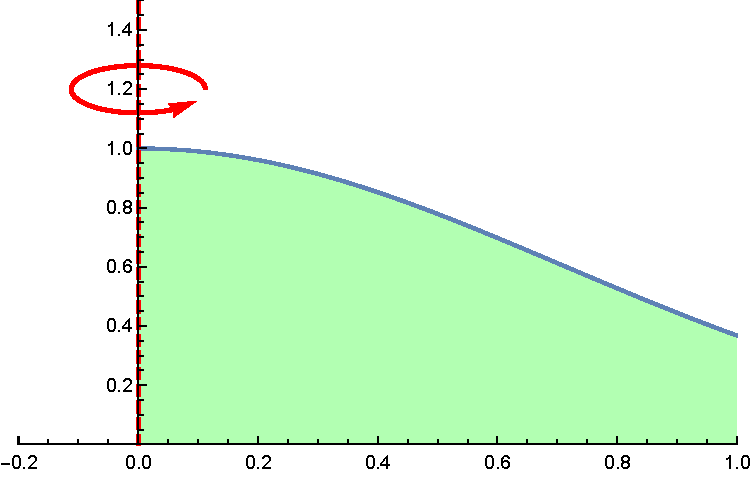
\includegraphics[width=0.4\textwidth]{Figures/volshexp.pdf}
        \caption{Region for Example \ref{e:volshexp}.}
        \label{f:volshexp}
    \end{figure}
    
    \begin{solution}
        \[V = 2\pi\int_{0}^{1} x e^{-x^{2}} \, dx = \pi \left( 1 - \frac{1}{e} \right)\]
    \end{solution}
\end{example}

\begin{example}
    \label{e:volshwrty}$R = \left\{ (x,y) \ | \ 0 \leq x \leq 3y^{2}, 0 \leq y \leq 1 \right\}$ about $y = -2$
    \begin{figure}[htbp]
        \centering
            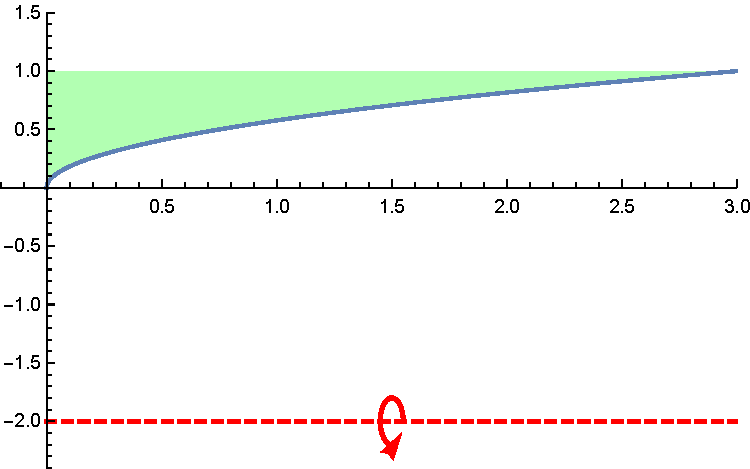
\includegraphics[width=0.4\textwidth]{Figures/volshwrty.pdf}
        \caption{Region for Example \ref{e:volshwrty}.}
        \label{f:volshwrty}
    \end{figure}
    
    \begin{solution}
        \[V = 2\pi\int_{0}^{1} (y+2)\cdot 3y^{2} \, dy = \frac{11\pi}{2}\]
    \end{solution}
\end{example}

\begin{example}
    \label{e:vol-shell-two-func-height}
    \(R = \left\{ (x,y) \ | \ 0 \leq x \leq 2, x \leq y \leq \sqrt{2x} \right\}\)
    \begin{figure}[htbp]
        \centering
            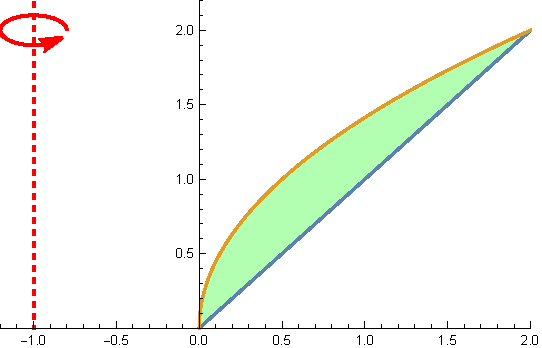
\includegraphics[width=0.4\textwidth]{Figures/volshtwofunc.pdf}
        \caption{Region for Example \ref{e:vol-shell-two-func-height}.}
        \label{f:vol-shell-two-func-height}
    \end{figure}
    \begin{solution}
        \[V = 2\pi \int_{0}^{2} (x + 2)(\sqrt{2x} - x) \, dx =  \left(\frac{2}{3} \sqrt{2} x^{3/2}+\frac{2}{5} \sqrt{2} x^{5/2}-\frac{x^3}{3}-\frac{x^2}{2}\right)\Bigg|_{0}^{2} = \frac{12\pi}{5}\]
    \end{solution}
\end{example}


\section{Physical Applications}
\setcounter{figure}{0}
\begin{itemize}
    \item Focusing on work, defined by $W = Fd$ in either J or ft $\cdot$ lb
    \item This is fine if force is constant, just multiply
    \item If $F$ not constant? Pretend it is over small distance $\Delta x$, take $\Delta x \to 0$
    \item $\displaystyle W = \int_{a}^{b} F(x) \, dx$
\end{itemize}

\subsection{Hooke's Law}
\begin{itemize}
    \item Force needed to stretch or compress a spring $x$ m or ft past its natural length is proportional to $x$, i.e. $F = kx$ where $k$ is the spring constant
    \item Only applies to relatively short distances
    \item Be careful with units and what the problem gives you
\end{itemize}

\begin{example}
    \label{e:workgivenforce}If it takes 300 N of force to compress a spring 5 m from its natural length, find the work done in compressing it one more meter.    
    
    \begin{solution}
        $k(5) = 300 \Rightarrow k = 60$ so the work done is
        \[W = \int_{5}^{6} 60x \, dx = 30x^{2}\Big|_{5}^{6} = 330 \text{ J}\]
    \end{solution}
\end{example}

\begin{example}
    \label{e:workgivenwork}If it takes 0.5 J of work to stretch a spring 20 cm past its natural length, find how much force is needed to stretch it 5 cm past its natural length.
        
    \begin{solution}
        \[0.5 = \int_{0}^{.2} kx \, dx \Rightarrow 0.5 = \frac{kx^{2}}{2}\Big|_{0}^{.2} \Rightarrow 0.5 =  0.02k \Rightarrow k = 25 \]
        so the force needed is $F = 25(0.05) = 1.25 \text{ N}$
    \end{solution}
\end{example}

\subsection{Rope and Weight}
\begin{itemize}
    \item $W_{\text{total}} = W_{\text{weight}} + W_{\text{rope}}$
    \item For weight just need $W = Fd$ \faSmile
    \item For rope need calculus \faMeh
\end{itemize}

\begin{example}
    \label{e:workropeandweight} A 10 m rope is hanging off of a tall building. The rope has constant density and has a mass of 2 kg. It has a 5 kg weight at the end. How much work is done in pulling up the rope and the weight?    
    
    \begin{solution}
        The density of the rope is $\rho = \frac{2}{10} = \frac{1}{5}$ kg/m. Let $g$ be acceleration due to gravity. Then the force required to lift an object of mass $m$ is $mg$. Let $y$ be the rope that has been pulled up; so $(10 - y)$ m of rope is still hanging with mass $\frac{1}{5}(10-y)$ kg, requiring $\frac{1}{5}(10-y)g$ N of force to lift. The total work done is then
        \[W = 10\cdot 5g + \int_{0}^{10} \frac{1}{5}(10-y)g \, dy = 60g \approx 588\text{ J}\] 
    \end{solution}  
\end{example}

\subsection{Draining Tanks}
\begin{itemize}
       \item Density of water: $\rho = 1000$ kg/m\textsuperscript{3}
       \item Divide up waters into layers with thickness $\Delta y$, volume of $i$\textsuperscript{th} layer is $A(y) \Delta y$ where $A(y)$ is the cross-sectional area at depth $y$ in the tank
       \item Calculate force required to lift, multiply by distance to get out to get work done
\end{itemize}

\begin{example}
    \label{e:worktriangletrough}A triangular trough with length 3 m, length 2 m, and height 1 m is full of water. How much work is done pumping all of the water out the top of the tank?       
    \begin{figure}[htbp]
        \centering
        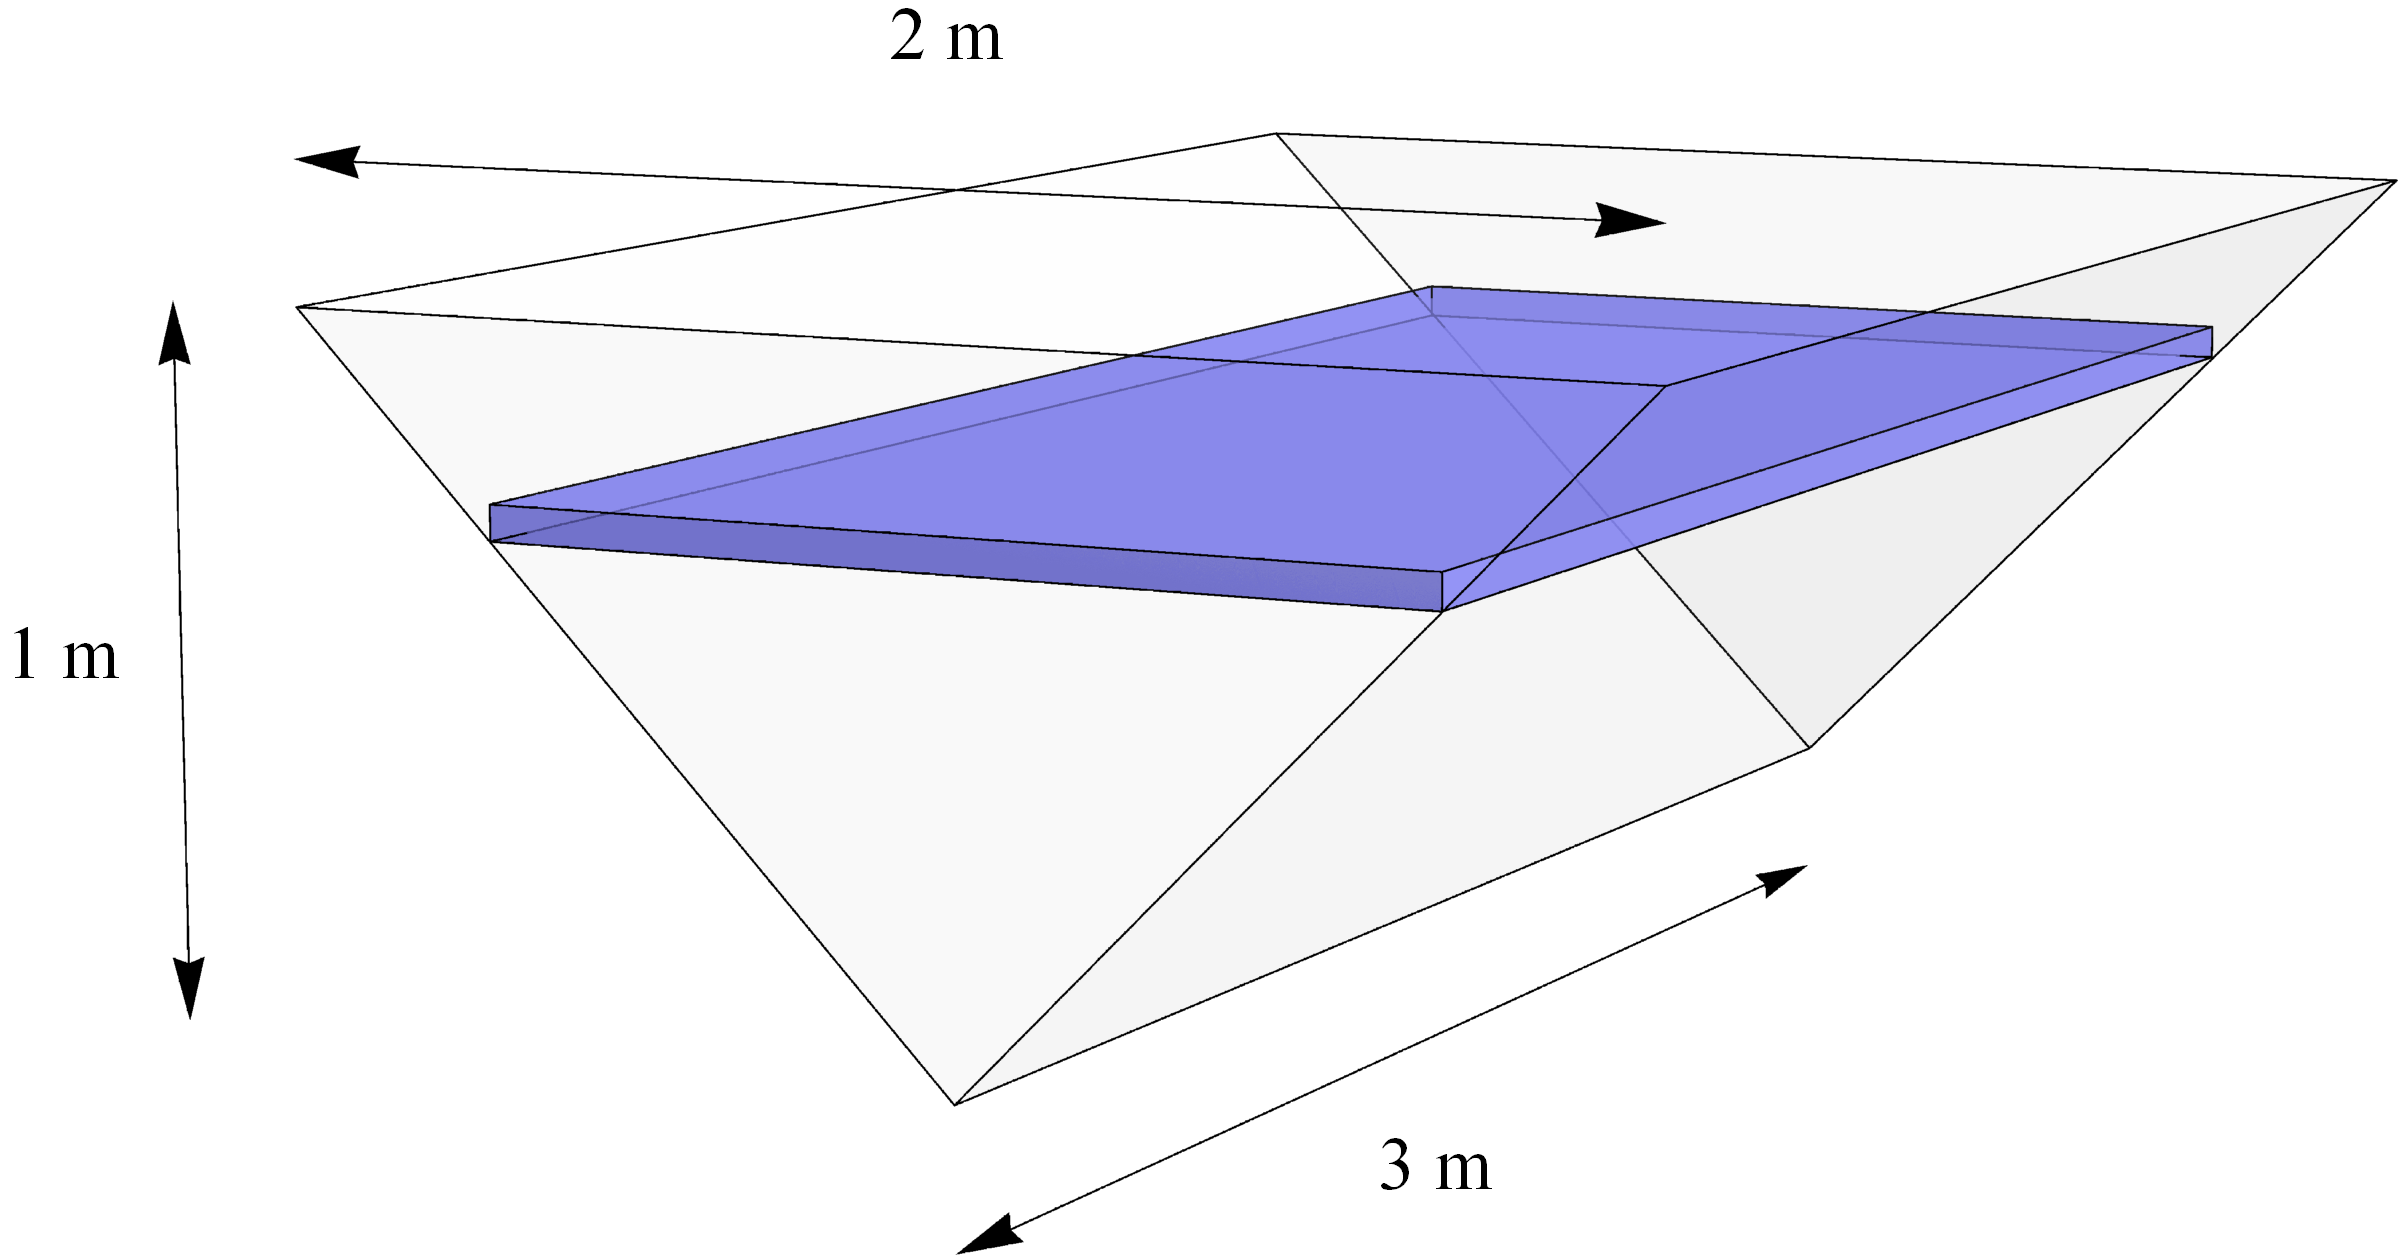
\includegraphics[width=0.5\textwidth]{Figures/prismtank.png}
        \caption{Trough in Example \ref{e:worktriangletrough}.}
        \label{f:worktriangletrough}
    \end{figure}
    
    \begin{solution}
        \begin{itemize}
            \item Layer is rectangular box at depth $y$ in the tank from the top with width $w$, length 3, and height $\Delta y$
            \item Need $w$ in terms of $y$
            \begin{itemize}
                \item By similar triangles, $\frac{w}{1-y} = \frac{2}{1} \Rightarrow w = 2(1-y)$
            \end{itemize}
        \end{itemize}
        Then we have
        \begin{align*}
            V_{\text{layer}} &= 3 \cdot 2(1-y)\Delta y = 6(1-y)\Delta y \text{ m\textsuperscript{3}}\\
            m_{\text{layer}} &= 6000(1-y)\Delta y \text{ kg}\\
            F_{\text{layer}} &= 6000g(1-y)\Delta y \text{ N}\\
            W_{\text{layer}} &= 6000g(1-y)y \Delta y \text{ J}
        \end{align*}
        Add up the work done on each layer, take $\Delta y \to 0$ to get
        \[
            W = \int_{0}^{1} 6000g(1-y)y \, dy = 1000g \approx 9807 \text{ J}
        \]
    \end{solution}
\end{example}

\begin{example}
    \label{e:workhemisphere} A bowl in the shape of a hemisphere with radius 0.2 m is filled with water. How much work is done pumping the water out of the top of the bowl?
    \begin{figure}[htbp]
        \centering
            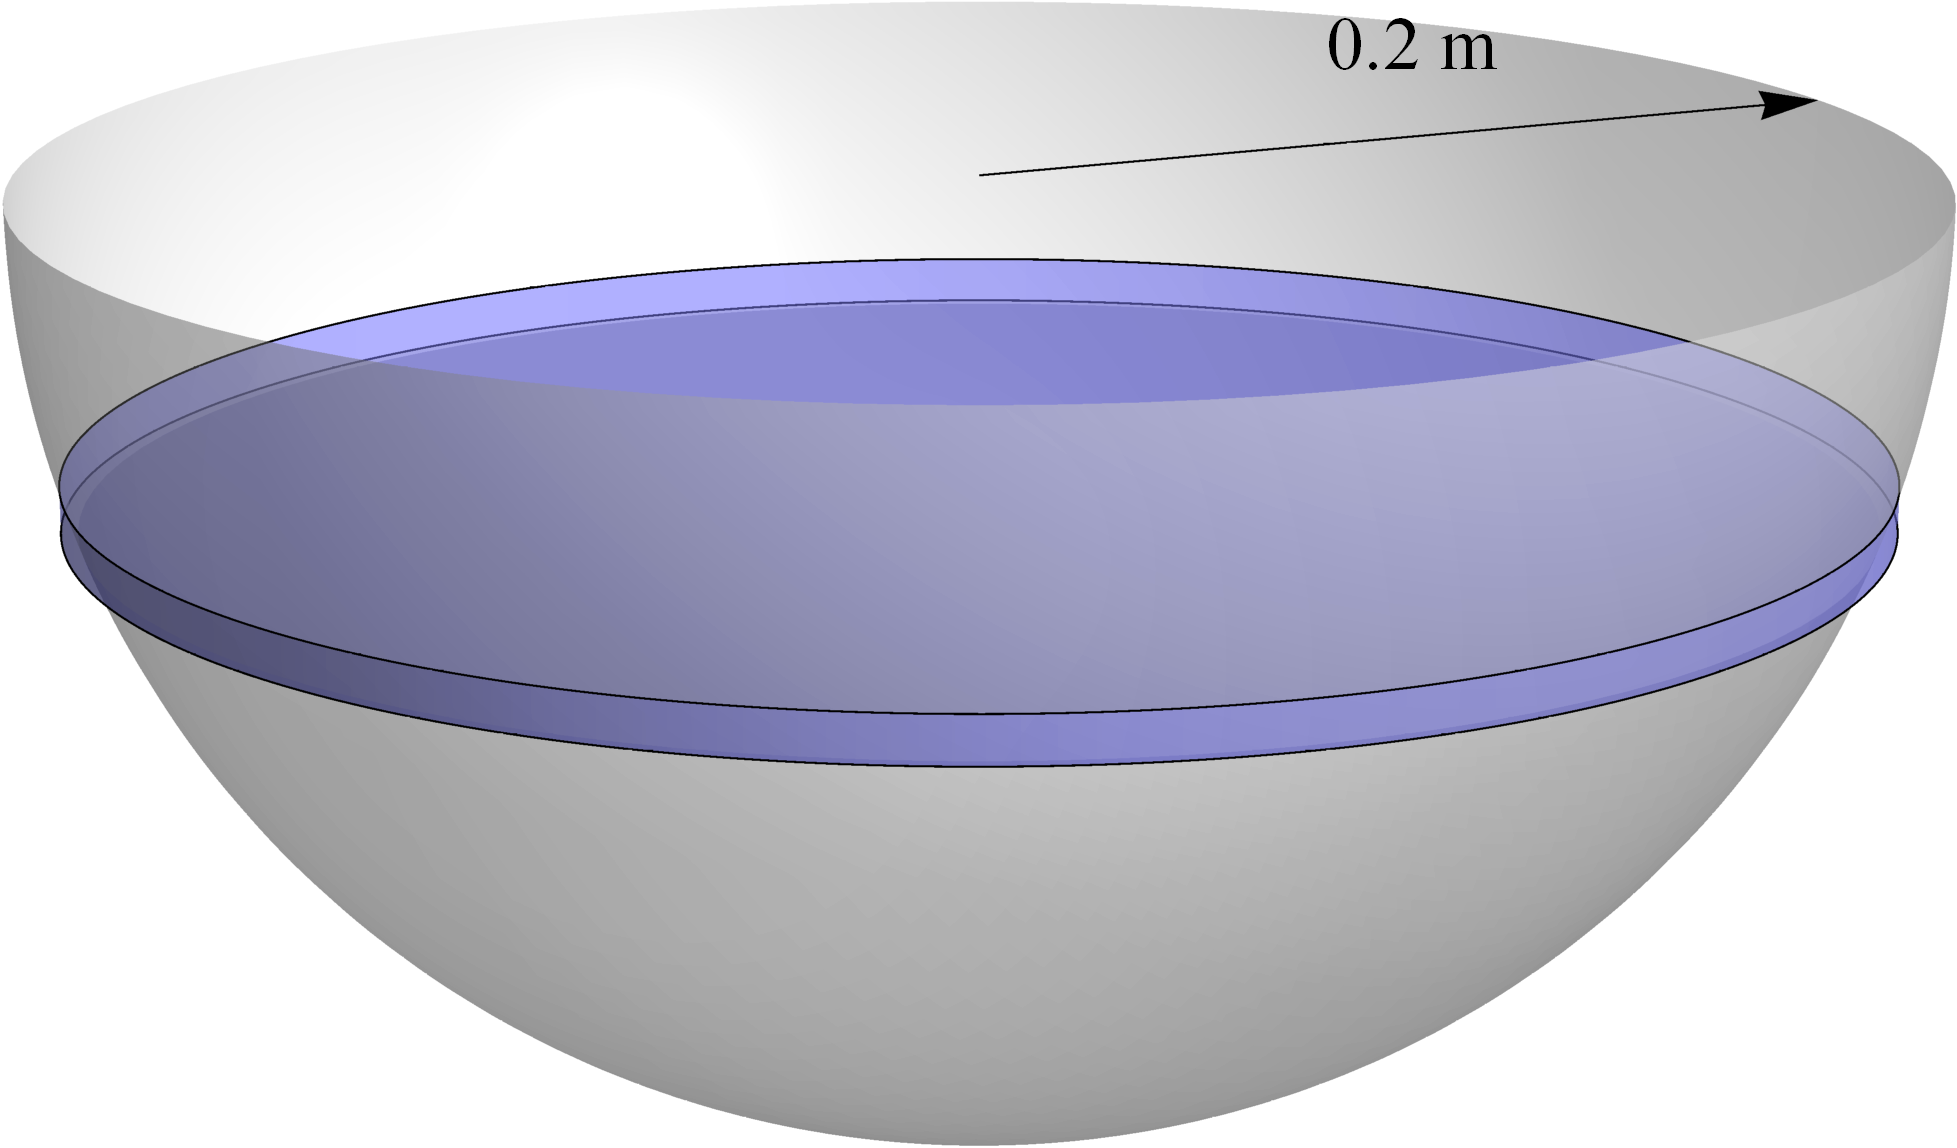
\includegraphics[width=0.4\textwidth]{Figures/workbowl.png}
        \caption{Bowl in Example \ref{e:workhemisphere}.}
        \label{f:workhemisphere}
    \end{figure}
    
    \begin{solution}
        \begin{itemize}
            \item Center bowl at origin, positive $y$ down
            \item $V_{\text{layer}} = \pi r^{2} h = \pi r^{2} \Delta y$
            \item Make equation of circumference $x^{2} + y^{2} = (0.2)^{2} \Rightarrow r = x = \sqrt{0.04 - y^{2}}$
        \end{itemize}
        So now
        \begin{align*}
            V_{\text{layer}} &= \pi (0.04 - y^{2}) \Delta y \text{ m\textsuperscript{3}}\\
            m_{\text{layer}} &= 1000 \pi (0.04 - y^{2}) \Delta y \text{ kg}\\
            F_{\text{layer}} &= 1000g \pi (0.04 - y^{2}) \Delta y \text{ N}\\
            W_{\text{layer}} &= 1000g \pi (0.04 - y^{2})y \text{ J}
        \end{align*}
        Add up the work done on each layer, take $\Delta y \to 0$ to get
        \[W = \int_{0}^{0.2} 1000g \pi (0.04 - y^{2})y = 0.4\pi g \approx  12.3\text{ J}\]
    \end{solution}
\end{example}

\newpage\thispagestyle{firstofchapter}
\chapter{More Integration Methods}
\section{Integration by Parts}
\setcounter{figure}{0}

Based on the Product Rule for derivatives:
\begin{align*}
    \frac{d}{dx} u(x) v(x) &= u(x)\frac{dv}{dx} + v(x) \frac{du}{dx}\\
    \intertext{Integrating both sides with respect to $x$ we get}
    u(x)v(x) &= \int u(x)\frac{dv}{dx} \, dx + \int v(x) \frac{du}{dx} \, dx\\
    uv &= \int u \, dv + \int v \, du\\
    \intertext{which gives us}
    \int u \, dv &= uv - \int v\, du
\end{align*}
which is the \textbf{integration by parts} formula. Note that we are \textit{kind of} cancelling out the \(dx\) differentials. We can say \(u'(x) dx = du\) and \(v'(x) dx = dv\) like we do for substitution.
\begin{itemize}
    \item Idea is to break down a hard integral into an easy one
    \item $u$ should usually be a function whose derivative is "simpler"
    \item $dv$ should be something we can integrate
\end{itemize}

\subsection{Indefinite Integrals}
\begin{example}\label{e:ibpexp}
Evaluate the integral: $\displaystyle \int x e^{x}\, dx$

\begin{solution}
    Let $u = x \Rightarrow du = dx$, $dv = e^{x}\, dx \Rightarrow v = e^{x}$;
    \[\int x e^{x}\, dx = x e^{x} - \int e^{x}\, dx = x e^{x} - e^{x} + C\]
\end{solution}
\end{example}

\begin{example}\label{e:ibpexp3x}
Evaluate the integral: $\displaystyle \int x^{3} e^{x}\, dx$

\begin{solution}
    Instead of integration by parts three times \faMeh \ we will use the Tabular Method \faSmile
    
    \begin{table}[htbp]
    	\centering
    	\caption{Tabular method for Example \ref{e:ibpexp3x}.}
    	\begin{tabular}{ccc}
    		\hline
    		$+/-$ & $u$ & $dv$ \\ \hline
    		$+$ & $x^{3}$ & $e^{x}$ \\
    		$-$ & $3x^{2}$ & $e^{x}$ \\
    		$+$ & $6x$ & $e^{x}$ \\
    		$-$ & $6$ & $e^{x}$ \\
    		$+$ & $0$ & $e^{x}$ \\ \hline
    	\end{tabular}
    \end{table}
    \[\int x^{3} e^{x}\, dx = x^{3}e^{x} - 3x^{2} e^{x} + 6x e^{x} - 6e^{x} + C\]
\end{solution}
\end{example}

\begin{example}\label{e:ibp-x3lnx}
    Evaluate the integral: $\displaystyle \int x^{3} \ln x \, dx$
    \begin{solution}
        At first this looks like another we will need to do more than once but it's fine \faSmile; let $u = \ln x \Rightarrow du = \frac{1}{x}\, dx$, $dv = x^{3} \, dx \Rightarrow v = \frac{x^{4}}{4}$. So that $v$ looks worse now but\dots
        \begin{align*}
            \int x^{3} \ln x \, dx  &= \frac{x^{4}\ln x}{4} - \int \frac{x^{3}}{4} \, dx \\
                                    &= \frac{x^{4}\ln x}{4} - \frac{x^{4}}{16} + C
        \end{align*}
    \end{solution}
\end{example}

\begin{example}\label{e:ibp-expsin}
    Evaluate the integral: $\displaystyle \int e^{x}\sin x \, dx$
    
    \begin{solution}
        Can do either way, but we will let $u = e^{x} \Rightarrow dx = e^{x} \, dx$, $dv = \sin x \, dx \Rightarrow v = -\cos x$. This gives
        \begin{align*}
            \int e^{x}\sin x \, dx  &= -e^{x}\cos x + \int e^{x}\cos x \, dx
            \intertext{but we need to integrate by parts again to get}
            \int e^{x}\sin x \, dx  &= -e^{x}\cos x + e^{x} \sin x - \int e^{x} \sin x \,dx 
        \end{align*}
        \ldots but now we are back where we started. But we can add the desired integral to both sides!
        \begin{align*}
            2 \int e^{x}\sin x \, dx &= -e^{x}\cos x + e^{x} \sin x \\
            \int e^{x}\sin x \, dx &= \frac{1}{2}\left(e^{x} \sin x -e^{x}\cos x  \right) + C
        \end{align*}
    \end{solution}
\end{example}

\begin{example}\label{e:ibplnx}
    Evaluate the integral: $\displaystyle \int \ln x \, dx$
    
    \begin{solution}
        Use $u = \ln x \Rightarrow du = \frac{1}{x}\, dx$, $dv = dx \Rightarrow v = x$:
        \begin{align*}
            \int \ln x \, dx = x\ln x - \int x\cdot \frac{1}{x}\, dx = x\ln x - \int dx = x\ln x - x + C
        \end{align*}
    \end{solution}
\end{example}

\subsection{Definite Integrals}
In general
\[\int_{a}^{b} u \, dv = uv\bigg|_{a}^{b} - \int_{a}^{b} v\, du\]
\begin{example}\label{e:ibpdefintexp}
    Evaluate the integral: $\displaystyle \int_{0}^{1} (x+ 2) e^{-x} \, dx$
    
    \begin{solution}
        Let $u = x + 2 \Rightarrow du = dx$, $dv = e^{-x}\, dx \Rightarrow v = -e^{-x}$:
        \begin{align*}
            \int_{0}^{1} (x+ 2) e^{-x} \, dx    &= -(x+2)e^{-x}\bigg|_{0}^{1} + \int_{0}^{1} e^{-x}\, dx\\
                                                &= 3 - \frac{4}{e}
        \end{align*}
    \end{solution}
\end{example}

\begin{example}\label{e:ibpdefintinvsin}
    Evaluate the integral: $\displaystyle \int_{0}^{1/2} \sin^{-1} x \, dx$
 
\begin{solution}
        Use $u = \sin^{-1} x \Rightarrow du = \frac{1}{\sqrt{1 - x^{2}}} \, dx$, $dv = dx \Rightarrow v = x$;
        \begin{align*}
            \int_{0}^{1/2} \sin^{-1} x \, dx    &= x\sin^{-1} x \bigg|_{0}^{1/2} + \int_{0}^{1/2} \frac{x}{\sqrt{1 - x^{2}}} \, dx \\
                                                &= -1 + \frac{\sqrt{3}}{2} + \frac{\pi}{12}
        \end{align*}
\end{solution}
\end{example}

\section{Trigonometric Integrals}
\setcounter{figure}{0}
\subsection{Sine and Cosine Functions}
\begin{itemize}
    \item Odd power of sine or cosine \faSmile
    \begin{itemize}
        \item Split off one factor of odd power
        \item Substitution; may need Pythagorean identity
    \end{itemize}
    \item Only even powers? \faMeh
    \begin{itemize}
        \item Will likely need half-angle identity
    \end{itemize}
\end{itemize}

\begin{example}\label{e:trigint-sin3}
    Evaluate the integral: $\displaystyle \int \sin^{3} x\, dx$
    
    \begin{solution}
        \begin{align*}
            \int \sin^{3} x\, dx &= \int \sin^{2} x \sin x \, dx = \int \left( 1 - \cos^{2} x \right) \sin x \, dx
            \intertext{Now use $u = \cos x \Rightarrow du = -\sin x \, dx$}
            \int \left( 1 - \cos^{2} x \right) \sin x \, dx &= -\int  \left( 1 - u^{2} \right)\, du = -u + \frac{1}{3} u^{3} + C\\
                                 &= -\cos x + \frac{1}{3}\cos^{3} x + C
        \end{align*}
    \end{solution}
\end{example}

\begin{example}\label{e:trigint-cos4}
    Evaluate the integral: $\displaystyle \int \cos^{4} x\, dx$
    
    \begin{solution}
        \begin{align*}
            \int \cos^{4} x\, dx    &= \int \left( \cos^{2} x \right)^{2} \, dx = \int \left( \tfrac{1}{2}\left( 1 + \cos 2x \right) \right)^{2} \, dx \\
                                    &= \frac{1}{4}\int \left( 1 + 2\cos 2x + \cos^{2} 2x \right)\, dx \\
                                    &= \frac{1}{4}\left( x + \sin 2x \right) + \frac{1}{4} \int \cos^{2}2x \, dx\\
                                    &= \frac{1}{4}\left( x + \sin 2x \right) + \frac{1}{8} \int \left( 1 + \cos 4x \right)\, dx \\
                                    &= \frac{1}{4}\left( x + \sin 2x \right) + \frac{1}{8} x + \frac{1}{32}\sin 4x + C\\
                                    &= \frac{3}{8}x + \frac{1}{4}\sin 2x + \frac{1}{32}\sin 4x + C
        \end{align*}
    \end{solution}
\end{example}

\subsection{Tangent and Secant}
\begin{itemize}
    \item Even secant or odd tangent with secant? \faSmile
    \begin{itemize}
        \item Even secant: split off $\sec^{2}x$ for $du$
        \item Odd tangent with secant: split off $\sec x \tan x$ for $du$
    \end{itemize}
    \item Otherwise \faMeh
    \begin{itemize}
        \item Depends on rest of function
    \end{itemize}    
\end{itemize}

\begin{example}\label{e:trigint-sec4}
    Evaluate the integral: $\displaystyle \int \sec^{4} x\, dx$.

\begin{solution}
        \begin{align*}
            \int \sec^{4} x\, dx    &= \int \sec^{2} x \sec^{2} x \, dx = \int \left( 1 + \tan^{2} x \right) \sec^{2} x \, dx
            \intertext{With $u = \tan x \Rightarrow du = \sec^{2} x \, dx$ we get}
            \int \left( 1 + \tan^{2} x \right) \sec^{2} x \, dx &= \int \left( 1 + u^{2} \right)\, du\\
            &= u + \frac{1}{3} u^{3} + C \\
            &= \tan x + \frac{1}{3}\tan^{3} x + C
        \end{align*}
\end{solution}
\end{example}

\begin{example}\label{e:trigint-tan3sec3}
    Evaluate the integral: $\displaystyle \int \tan^{3}x \sec^{3} x\, dx$.

\begin{solution}
    \begin{align*}
        \int \tan^{3}x \sec^{3} x\, dx
            &= \int \left( \sec^{2} x - 1 \right)\sec^{2} x \sec x \tan x \, dx
        \intertext{With $u = \sec x \Rightarrow du = \sec x \tan x \, dx$:}
        \int \left( \sec^{2} x - 1 \right)\sec^{2} x \sec x \tan x \, dx &= \int \left( u^{2} - 1 \right) u^{2}\, du\\
            &= \frac{1}{5}u^{5} - \frac{1}{3}u^{3} + C \\
            &= \frac{1}{5}\sec^{5} x -\frac{1}{3} \sec^{3} x + C
    \end{align*}
\end{solution}
\end{example}

\begin{example}\label{e:trigintsectandefint}
    Evaluate the integral: $\displaystyle \int_{\pi / 4}^{\cos^{-1}\frac{1}{4}} \tan^{2} \theta \sec^{2}\theta \, d\theta$
\begin{solution}
       
        Let $u = \tan x \Rightarrow du = \sec^{2} x \, dx, u\left(\cos^{-1}\frac{1}{4}\right) = \sqrt{15}, u(\pi / 4) = 1$
        \[
            \int_{\pi / 4}^{\cos^{-1}\frac{1}{4}} \tan^{2} \theta \sec^{2}\theta \, d\theta = \int_{1}^{\sqrt{15}} u^{2} \, du = \frac{1}{3} u^{3} \bigg|_{1}^{\sqrt{15}} = \frac{15\sqrt{15} - 1}{3}
        \]    
\end{solution}
\end{example}

\begin{example}\label{e:trigintsec3}
    Evaluate the integral: $\displaystyle \int \sec^{3}x \, dx$
    
    \begin{solution}
        We will need integration by parts with $u = \sec x \Rightarrow du = \sec x \tan x$ and $dv = \sec^{2} x \Rightarrow v = \tan x$:
        \begin{align*}
            \int \sec^{3}x \, dx &= \sec x \tan x - \int \tan^{2} x \sec x \, dx
            \intertext{with the identity $\tan^{2} x = \sec^{2} x - 1$ we have}
            \int \sec^{3}x \, dx &= \sec x \tan x - \int \left( \sec^{2} x - 1 \right)\sec x \, dx\\
            \int \sec^{3}x \, dx &= \sec x \tan x - \left( \int \sec^{3} x \, dx - \int \sec x \, dx \right)
            \intertext{so again we have the desired integral on both sides of the equation. Adding it to both sides gives us}
            2 \int \sec^{3}x \, dx &= \sec x \tan x + \int \sec x \, dx \text{, so now}\\
            \int \sec^{3}x \, dx &= \frac{1}{2}\left(\sec x \tan x + \ln | \sec x + \tan x | \right) + C
        \end{align*}
    \end{solution}   
\end{example}

\subsection{Other cases}
\begin{itemize}
    \item May need power reduction formulas (see text)
    \item May use product-to-sum formulas
\end{itemize}

\section{Trigonometric Substitution}
\setcounter{figure}{0}
\begin{table}[htbp]
	\centering
	\caption{Trig subs}
	\begin{tabular}{lll}		
		\textbf{Expression} & \textbf{Substitution} & $\bm{\theta}$ \\ \hline
		$a^{2} - x^{2}$     & $x = a \sin \theta$   & $-\pi/2 \leq \theta \leq \pi /2$ \\[0.75ex]
		$a^{2} + x^{2}$     & $x = a \tan \theta$   & $-\pi/2 < \theta < \pi /2$ \\[0.75ex]
		$x^{2} - a^{2}$     & $x = a \sec \theta$   & $0 \leq \theta < \pi /2$, $\pi \leq \theta < 3\pi/2$ \\ 
	\end{tabular}
\end{table}

\subsection{Indefinite Integrals}
\begin{example}\label{e:trigsubtan}
    Evaluate the integral: $\displaystyle \int \frac{1}{\sqrt{x^{2} + 1}}\, dx$
    
    \begin{solution}
        Use $x = \tan \theta \Rightarrow dx = \sec^{2} \theta\, d\theta$, $\sqrt{x^{2} + 1} = \sec \theta$:
        \begin{align*}
            \int \frac{1}{\sqrt{x^{2} + 1}}\, dx &= \int \sec \theta \, d\theta = \ln \left| \sec \theta + \tan \theta \right| + C\\
            &= \ln \left| \sqrt{x^{2} + 1} + x \right| + C\\
        \end{align*}
    \end{solution}
\end{example}

\begin{example}\label{e:trigsubsec}
    Evaluate the integral: $\displaystyle \int \frac{\sqrt{x^{2} - 25}}{x}\, dx$
    
    \begin{solution}
        Use $x = 5\sec \theta \Rightarrow dx = 5\sec \theta \tan \theta \, d\theta$, $\sqrt{x^{2} - 25} = 5\tan \theta$:
        \begin{align*}
            \int \frac{\sqrt{x^{2} - 25}}{x}\, dx &= \int 5 \tan^{2} \theta \, d\theta = 5 \int \left( \sec^{2} \theta - 1 \right)\, d\theta \\        
            &= 5 \left( \tan \theta - \theta \right) + C \\
            &=  \sqrt{x^{2} - 25} - 5\sec^{-1} \left(\frac{x}{5}\right)  + C
        \end{align*}
    \end{solution}
\end{example}

\begin{example}\label{e:trigsubsin}
    Evaluate the integral: $\displaystyle \int \frac{1}{x^{2} \sqrt{1-x^{2}}}\, dx$
    
    \begin{solution}
        Use $x = \sin \theta \Rightarrow dx = \cos \theta \, d\theta$, $\sqrt{1 - x^{2}} = \cos \theta$:
        \begin{align*}
            \int \frac{1}{x^{2} \sqrt{1-x^{2}}}\, dx &= \int \csc^{2} \theta \, d\theta \\
            &= -\cot \theta + C \\
            &= -\frac{\sqrt{1-x^{2}}}{x} + C
        \end{align*}
    \end{solution}
\end{example}

\begin{example}\label{e:trigsubprelimsub}
    Evaluate the integral: $\displaystyle \int \! \frac{1}{(16 - 9x^{2})^{3/2}}\, dx$
    
    \begin{solution}
        We can't do a trig substitution just yet but we can do a regular substitution first. Let $u = 3x \Rightarrow du = 3 dx$ to get
        \[
            \int \! \frac{1}{(16 - 9x^{2})^{3/2}}\, dx = \frac{1}{3} \int \frac{1}{(16 - u^{2})^{3/2}} \, du
        \]
        Now we can do a trig substitution with $u = 4\sin \theta \Rightarrow du = 4\cos \theta$, $(16-u^{2})^{3/2} = (16\cos^{2} \theta)^{3/2} = 64\cos^{3} \theta$:
        \begin{align*}
            \frac{1}{3} \int \frac{1}{(16 - u^{2})^{3/2}} \, du &= \frac{1}{48}\int \sec^{2}\theta \, d\theta \\
            &= \frac{1}{48}\tan \theta + C \\
            &= \frac{u}{48\sqrt{16-u^{2}}} + C =  \frac{x}{16\sqrt{16-9x^{2}}} + C
        \end{align*}
    \end{solution}
\end{example}

\begin{example}\label{e:trigsubcompsq}
    Evaluate the integral: $\displaystyle \int \frac{1}{\sqrt{x^{2} + 4x + 8}}\, dx$
    
    \begin{solution}
        The polynomial in the denominator cannot be factored over $\mathbb{R}$ but we can complete the square to get $x^{2} + 4x + 8 = (x+2)^{2} + 4$. Now we can do a preliminary substitution with $u = x + 2 \Rightarrow du = dx$.
        \[
            \int \frac{1}{\sqrt{x^{2} + 4x + 8}}\, dx = \int \frac{1}{\sqrt{(x+2)^{2} + 4}} \, dx = \int \frac{1}{\sqrt{u^{2} + 4}}\, du
        \]
        Now we're good to go for a trig substitution with $u = 2\tan \theta \Rightarrow du = 2\sec^{2} \theta \, d\theta$, $u^{2} + 4 = 4\sec \theta$:
        \begin{align*}
            \int \frac{1}{\sqrt{u^{2} + 4}}\, du &= \int \sec \theta \, d\theta \\
            &= \ln |\sec \theta + \tan \theta| + C \\
            &= \ln \left| \frac{\sqrt{u^{2} + 4}}{2} + \frac{u}{2}\right| + C \\
            &= \ln \left| \frac{\sqrt{x^{2} + 4x + 8}}{2} + \frac{x + 2}{2}\right| + C\\
            &= \ln \left| \frac{1}{2}\left(\sqrt{x^{2} + 4x + 8} + x + 2\right)\right|\\
            &= \ln \left| \sqrt{x^{2} + 4x + 8} + x + 2\right| + \ln \frac{1}{2} + C\\
            &= \ln \left| \sqrt{x^{2} + 4x + 8} + x + 2\right| + D
        \end{align*}
    \end{solution}
\end{example}

\subsection{Definite Integrals}

\begin{example}\label{e:trigsubnotneed}
    Evaluate the integral: $\displaystyle \int_{0}^{1} x^{3}\sqrt{1-x^{2}} \, dx$
    
    \begin{solution}
        \faExclamationTriangle[solid] \ We do not need a trig sub here! But let's try it anyway and see what happens. Use $x = \sin \theta \Rightarrow dx = \cos \theta \, d\theta$, $\sqrt{1-x^{2}} = \cos \theta$; $1 = \sin \theta \Rightarrow \theta = \frac{\pi}{2}$, $0 = \sin \theta \Rightarrow \theta = 0$:
        \begin{align*}
            \int_{0}^{1} x^{3}\sqrt{1-x^{2}} \, dx &= \int_{0}^{\pi/2} \sin^{3}\theta \cos^{2}\theta \, d\theta \\
            &= \int_{0}^{\pi/2} \left( 1 - \cos^{2} \theta \right) \cos^{2}\theta \sin \theta \, d\theta
            \intertext{\ldots and now we need a substitution. \faMeh \ Use $u = \cos \theta \Rightarrow du = -\sin \theta \, d\theta$; $u(0) = 1, u(\pi/2) = 0$:}
            \int_{0}^{\pi/2} \left( 1 - \cos^{2} \theta \right) \cos^{2}\theta \sin \theta \, d\theta &=-\int_{1}^{0}\left( 1- u^{2} \right)u^{2} \, du = \frac{2}{15}
        \end{align*}
        But we could have avoided this at the beginning by letting $u = 1 - x^{2} \Rightarrow x^{2}= 1- u, du = -2x\, dx$; $u(0) = 1, u(1) = 0 $:
        \begin{align*}
            \int_{0}^{1} x^{3}\sqrt{1-x^{2}} \, dx &= -\frac{1}{2}\int_{1}^{0}(1-u)\sqrt{u}\, du = \frac{2}{15} \text{ \faSmile}
        \end{align*}
    \end{solution}
\end{example}

\begin{example}\label{e:trigsubdiv}
    Evaluate the integral: $\displaystyle \int_{0}^{1} \frac{x^{4}}{1+x^{2}} \, dx$
    
    \begin{solution}
        \faExclamationTriangle[solid] \ Note that again we really don't need a trig substitution. We can do some polynomial division first. But let's do a trig substitution anyway! Let $x = \tan \theta \Rightarrow dx = \sec^{2}\theta \, d\theta$, $1 + x^{2} = \sec^{2} \theta$, $1 = \tan \theta \Rightarrow \theta = \frac{\pi}{4}$, $0 = \tan \theta \Rightarrow \theta = 0$:
        \begin{align*}
            \int_{0}^{1} \frac{x^{4}}{1+x^{2}} \, dx &= \int_{0}^{\pi/4} \tan^{4} \theta \, d\theta = \int_{0}^{\pi/4} \tan^{2} \theta \tan^{2} \theta \, d\theta = \int_{0}^{\pi/4} \left( \sec^{2} \theta - 1 \right) \tan^{2} \theta \, d\theta \\
            &= \int_{0}^{\pi/4} \tan^{2} \theta \sec^{2} \theta\, d\theta  - \int_{0}^{\pi/4} \tan^{2} \theta \, d\theta = \int_{0}^{\pi/4} \tan^{2} \theta \sec^{2} \theta\, d\theta - \int_{0}^{\pi/4} \left( \sec^{2}\theta - 1 \right)\, d\theta \\
            \intertext{Using $u = \tan \theta \Rightarrow du = \sec^{2}\theta \, d\theta$, $u(\pi/4) = 1$, $u(0)= 0$ on the first integral gives}
            &= \int_{0}^{1} u^{2} \, du - \left( \tan x - x \right)\Big|_{0}^{\pi/4}  = \frac{1}{3} - \left( 1 - \frac{\pi}{4} \right) = \frac{\pi}{4} - \frac{2}{3}
        \end{align*}
        But that was a lot of work. \faMeh
    
        Instead we could have done some polynomial division!
        \[\frac{x^{4}}{1 + x^{2}} = x^{2} - 1 - \frac{1}{1+x^{2}}  \]
        We can integrate all of these as-is.
        \[\int_{0}^{1} \frac{x^{4}}{1+x^{2}} \, dx = \int_{0}^{1} \left( x^{2} - 1 - \frac{1}{1+x^{2}} \right) \, dx = \left( \frac{x^{3}}{3}  - x + \tan^{-1}x \right)\Bigg|_{0}^{1} = \frac{\pi}{4} - \frac{2}{3}\]
        That was much easier! \faSmile
    \end{solution}
    
\end{example}

\begin{example}\label{e:trigsubdintsec}
    Evaluate the integral: $\displaystyle \int_{5/2}^{5\sqrt{3}/2} \frac{x^{2}}{\sqrt{25 - x^{2}}} \, dx$
    
    \begin{solution}
        Use $x = 5\sin \theta \Rightarrow dx = 5 \cos \theta \, d\theta$, $\sqrt{25-x^{2}} = 5 \cos \theta$, $\frac{5}{2} = 5\sin \theta \Rightarrow \theta = \frac{\pi}{6}$, $\frac{5\sqrt{3}}{2} = 5\sin \theta \Rightarrow \theta = \frac{\pi}{3}$:
        \begin{align*}
            \int_{5/2}^{5\sqrt{3}/2} \frac{x^{2}}{\sqrt{25 - x^{2}}} \, dx &= 25 \int_{\pi/6}^{\pi/3} \sin^{2} \theta \, d\theta \\
            &= \frac{25}{2} \int_{\pi/6}^{\pi/3} \left( 1 - \cos 2\theta \right)\, d\theta \\
            &= \frac{25}{2} \left( \theta - \frac{1}{2}\sin 2\theta \right)\bigg|_{\pi/6}^{\pi/3} = \frac{25\pi}{12}
        \end{align*}
    \end{solution}
\end{example}

\begin{example}\label{e:trigsubtandefint}
    Evaluate the integral: $\displaystyle \int_{\sqrt{2}}^{\sqrt{6}} \frac{\sqrt{x^{2}+2}}{x^{2}} \, dx$
    \begin{solution}
        Use $x = \sqrt{2}\tan \theta \Rightarrow dx = \sqrt{2} \sec^{2} \theta \, d\theta$, $\sqrt{x^{2}+ 2} = \sqrt{2} \sec \theta$, $\sqrt{6} = \sqrt{2} \tan  \theta \Rightarrow \theta = \frac{\pi}{3}$, $\sqrt{2} = \sqrt{2} \tan  \theta \Rightarrow \theta = \frac{\pi}{4}$:
        \[
            \int_{\sqrt{2}}^{\sqrt{6}} \frac{\sqrt{x^{2}+2}}{x^{2}} \, dx = \int_{\pi/4}^{\pi/4} \frac{\sec^{3}\theta}{\tan^{2}\theta}\, d\theta
        \]
    Let's simplify this a little first:
    \[\frac{\sec^{3}\theta}{\tan^{2}\theta} = \frac{1}{\cos^{3}\theta} \frac{\cos^{2}\theta}{\sin^{2}\theta} = \frac{1}{\cos \theta} \frac{1}{\sin^{2}\theta} = \sec \theta \csc^{2}\theta = \sec \theta (1 + \cot^{2} \theta) = \sec \theta + \csc \theta \cot \theta\]
    Now we have
        \begin{align*}
            \int_{\pi/4}^{\pi/3} \frac{\sec^{3}\theta}{\tan^{2}\theta}\, d\theta &= \int_{\pi/4}^{\pi/3} \left( \sec \theta + \csc \theta \cot \theta \right) \, d\theta \\
            &= \left(\ln \left| \sec \theta + \tan \theta \right| - \csc \theta \right) \bigg|_{\pi/4}^{\pi/3} \\
            &= \sqrt{2}-\frac{2}{\sqrt{3}}-\ln \left(\sqrt{2}+1\right) + \ln\left(\sqrt{3}+2\right)
        \end{align*}
    \end{solution}
\end{example}



\section{Partial Fractions}
\setcounter{figure}{0}
\begin{itemize}
    \item For rational functions
    \item Fundamental Theorem of Algebra
    \begin{itemize}
        \item If $f$ is a polynomial with complex coefficients, then $f$ has a complex root
        \item This extends to factoring $f$ over linear complex factors        
    \end{itemize}
    \item If all coefficients of a polynomial are real, can be factored to linear and irreducible quadratic factors
\end{itemize}
\begin{table}[htbp]
	\centering
	\caption{Contributions to Decomposition}
	\begin{tabular}{ll}
		\textbf{Factor} & \textbf{Terms} \\ \hline \\[-1em]
        $(ax + b)$ & $\dfrac{A}{ax + b}$ \\[2.5ex]
        $(ax + b)^{n}, n \geq 2$ & $\dfrac{A_{1}}{ax + b} + \dfrac{A_{2}}{(ax + b)^{2}} + \cdots + \dfrac{A_{n}}{(ax + b)^{n}}$\\[2.5ex]
        $(ax^{2} + bx + c)$, $b^{2} - 4ac < 0$ & $\dfrac{Ax + B}{ax^{2} + bx + c}$ \\[2.5ex]
		$(ax^{2} + bx + c)^{n}$, $b^{2} - 4ac < 0$, $n \geq 2$ & $\dfrac{A_{1}x + B_{1}}{ax^{2} + bx + c} + \dfrac{A_{2}x + B_{2}}{(ax^{2} + bx + c)^{2}} + \cdots + \dfrac{A_{n}x + B_{n}}{(ax^{2} + bx + c)^{n}}$ \\ \hline
	\end{tabular}
\end{table}

\subsection{Distinct Linear Factors}
\begin{itemize}
    \item In these cases its easier to choose values of $x$ to plug in and make terms disappear
    \item Will use shortcut:
    \[\int \frac{1}{ax + b} \, dx = \frac{1}{a} \ln |ax + b| + C  \]
    \item[{\faExclamationTriangle[solid]}] \ Do not overuse the above rule; general rule is $\int \frac{g'(x)}{g(x)}\, dx = \ln |g(x)| + C$
    \item[{\faExclamationTriangle[solid]}] \ In general $\int \frac{1}{g(x)}\, dx \neq \ln |g(x)| + C$    
\end{itemize}

\begin{example}\label{e:parfracdlin}
    Evaluate the integral: $\displaystyle \int \frac{x+18}{x^2+x-12} \, dx$
    
    \begin{solution}
        \begin{align*}
            \frac{x+18}{x^2+x-12} &= \frac{A}{x-3} + \frac{B}{x+4}\\[2ex]
            x + 18 &= A(x+4) + B(x-3)
        \end{align*}
        With $x=3$ we get $21 = 7A \Rightarrow A = 3$; with $x=-4$ we get $14 = -7B \Rightarrow B = -2$. So we integrate
        \[\int \left( -\frac{2}{x+4} + \frac{3}{x-3} \right)\, dx = -2\ln |x  + 4| + 3 \ln |x - 3| + C\]
    \end{solution}
\end{example}

\begin{example}\label{e:parfracimprop}
    Evaluate the integral: $\displaystyle \int \frac{2x^{3}- 5 x^{2} - 8x + 9}{x^{2} - 3x - 4} \, dx$
    
    \begin{solution}
        This is an "improper" \faFrown \ rational function, so we need polynomial division first. Dividing we get
        \[\frac{2x^{3}- 5 x^{2} - 8x + 9}{x^{2} - 3x - 4} = 2x + 1 + \frac{3x + 13}{x^{2} - 3x - 4} = 2x + 1 + \frac{3x + 13}{(x-4)(x+1)}\]
        Now we decompose the "proper" \faMeh \ rational function.
        \begin{align*}
            \frac{3x + 13}{(x-4)(x+1)} &= \frac{A}{x-4} + \frac{B}{x+1} \\[2ex]
            3x + 13 &= A(x+1) + B(x-4)
        \end{align*}
        With $x = -1$ we have $10 = -5B \Rightarrow B = -2$; with $x = 4$ we have $25 = 5A \Rightarrow A = 5$. So we integrate
        \[\int \left( 2x + 1 +  \frac{5}{x-4} - \frac{2}{x+1}\right) \, dx = x^{2} + x + 5\ln |x-4| -2\ln |x + 1| + C\]  
    \end{solution}
\end{example}

\begin{example}\label{e:parfracdlin2}
    Evaluate the integral: $\displaystyle \int \frac{4x^{2} + x + 1}{x^{3} - x} \, dx$
    
    \begin{solution}
        \begin{align*}
            \frac{4x^{2} + x + 1}{x^{3} - x} &= \frac{A}{x} + \frac{B}{x-1} + \frac{C}{x+1}\\[2ex]
            4x^{2} + x + 1 &= A(x-1)(x+1) + Bx(x+1) + Cx(x-1)
        \end{align*}
        With $x = 0$ we have $1 = -A \Rightarrow A = -1$; with $x=1$ we have $6 = 2B \Rightarrow B = 3$; with $x = -1$ we have $4 = 2C \Rightarrow C = 2$. So we integrate
        \[\int \left( -\frac{1}{x} + \frac{3}{x-1} + \frac{2}{x+1} \right)\, dx = -\ln |x| + 3\ln |x - 1| + 2\ln |x + 1| + K\]
    \end{solution}    
    \begin{commentary}
        \faExclamationTriangle[solid] \ Note that we need a different constant as the usual $C$ has already been used.
    \end{commentary}
    \end{example}

\subsection{Repeated Linear Factors}
\begin{example}\label{e:parfracreplin}
    Evaluate the integral: $\displaystyle \int \frac{4x + 11}{(x + 4)^{2}} \, dx$
    
    \begin{solution}
        \begin{align*}
            \int \frac{4x + 11}{(x + 4)^{2}} &= \frac{A}{x + 4} + \frac{B}{(x + 4)^{2}}\\[2ex]
            4x + 11 &= A(x+4) + B
        \end{align*}
        With $x = -4$, we have $-5 = B$ \faSmile \ ; with $x = 0$ we have $11 = 4A + B = 4A - 5 \Rightarrow A = 4$. So we integrate
        \[\int \left( \frac{4}{x + 4} - \frac{5}{(x + 4)^{2}} \right) \, dx = 4\ln |x + 4| + \frac{5}{x  + 4} + K\]
    \end{solution}
\end{example}

\begin{example}\label{e:parfracreplin2}    
    Evaluate the integral: $\displaystyle \int \frac{-4x^{2} + 27x - 32}{(x - 2)^{2} (x + 1)} \, dx$
    
    \begin{solution}
        \begin{align*}
            \frac{-4x^{2} + 27x - 32}{(x - 2)^{2} (x + 1)} &= \frac{A}{x-2} + \frac{B}{(x-2)^{2}} + \frac{C}{x + 1}\\[2ex]
            -4x^{2} + 27x - 32 & = A(x - 2)(x + 1) + B(x + 1) + C(x-2)^{2}
        \end{align*}
    
    With $x = 2$ we have $6 = 3B \Rightarrow B = 2$; with $x = -1$ we have $-63 = 9C \Rightarrow C = -7$; with $x = 0$ we have $-32 = -2A + 2 - 28 \Rightarrow A = 3$. So we integrate
    \[\int \left( \frac{3}{x-2} + \frac{2}{(x-2)^{2}} - \frac{7}{x + 1} \right)\, dx = 3\ln |x - 2| - \frac{2}{x - 2} - 7\ln |x + 1| + K\]
    \end{solution}
\end{example}

\subsection{Distinct Irreducible Quadratic Factors}
\begin{example}\label{e:parfracdirred}
    Evaluate the integral: $\displaystyle \int \frac{3x^{2} + 2x + 3}{3x\left( x^{2} + 1 \right)} \, dx$
    
    \begin{solution}
        \begin{align*}
            \frac{3x^{2} + 2x + 3}{3x\left( x^{2} + 1 \right)} &= \frac{A}{3x} + \frac{Bx + C}{x^{2} + 1}\\[2ex]
            3x^{2} + 2x + 3 &= A(x^{2} + 1) + 3(Bx + C)x
        \end{align*}
        With $x = 0$ we have $3 = A$ \faSmile \ ; with $x = 1$ we have $8 = 6 + 3B + 3C \Rightarrow 3B + 3C = 2$; with $x = -1$ we have $4 = 6 + 3B - 3C \Rightarrow 3B - 3C = -2$. So we need to solve the system    
        \begin{alignat*}{3}
            3B & {}+{} & 3C & {}={} &2 \\
            3B & {}-{} & 3C & {}={} -&2
        \end{alignat*}
        with solutions $B = 0, C = \frac{2}{3}$. So we integrate
        \[\int \left( \frac{1}{x} + \frac{2}{3(x^{2} + 1)} \right) \, dx = \ln |x| + \frac{2}{3} \tan^{-1}x  + K\]
    \end{solution}
\end{example}

\begin{example}\label{e:parfracdirred2}
    Evaluate the integral: $\displaystyle \int \frac{7x^{2} + 8x + 6}{(x + 1)(x^{2} + x + 1)} \, dx$
    
    \begin{solution}
        \begin{align*}
            \frac{7x^{2} + 8x + 6}{(x + 1)(x^{2} + x + 1)} &= \frac{A}{x + 1} + \frac{Bx + C}{x^{2} + x + 1}\\[2ex]
            7x^{2} + 8x + 6 & = A(x^{2} + x + 1) + (Bx + C)(x + 1)
        \end{align*}
        With $x = -1$ we have $5 = A$ \faSmile \ ; with $x = 0$ we have $6 = 5 + C \Rightarrow C = 1$; with $x = 1$ we have $21 = 15 + (B + 1)(2) \Rightarrow B = 2$. So we integrate
        \[\int \left( \frac{5}{x + 1} + \frac{2x + 1}{x^{2} + x + 1} \right)\, dx = 5\ln |x + 1| + \ln |x^{2} + x + 1| + K\]
    \end{solution}
\end{example}

\subsection{Repeated Irreducible Quadratic Factors}
\begin{example}\label{e:parfracrepirred}
    Evaluate the integral: $\displaystyle \int \frac{2x^{2} - x + 8}{(x^{2} + 4)^{2}} \, dx$
    
    \begin{solution}
        \begin{align*}
            \frac{2x^{2} - x + 8}{(x^{2} + 4)^{2}} &= \frac{Ax + B}{x^{2} + 4} + \frac{Cx + D}{(x^{2} + 4)^{2}}\\[2ex]
            2x^{2} - x + 8 &= (Ax + B)(x^{2} + 4) + Cx + D
        \end{align*}
        Here the plug in for \(x\) method results in a system of equations that is not pleasant to work by hand \faFrown:    
        \begin{alignat*}{7}
            x = 0 &: & {} {} &4B {} {}  & {}+{} &D &{}={} &8\\
            x = -1 &: &-5A {}+{} &5B {}-{} &C {}+{} &D &{}={} &11\\
            x = 1&: &5A {}+{} &5B {}+{} &C {}+{} &D &{}={} &9\\
            x = 2 &: &16A {}+{} &8B {}+{} &2C {}+{} &D  &{}={} &14
        \end{alignat*}
        This system has the solution set $A = 0, B = 2, C = -1, D = 0$. We can get this same solution set more easily by instead expanding the polynomial equation and matching coefficients:
        
        \begin{align*}
            2x^{2} - x + 8  &= (Ax + B)(x^{2} + 4) + Cx + D\\
                            &= Ax^{3} + Bx^{2} + (4A + C)x + (4B+D)
        \end{align*}
        Matching the coefficients (using 0 for any missing term) we get (freebies! \faSmile) \(A = 0, B = 2, C = -1\); then with \(B=2, 4B+D = 8 \Rightarrow D = 0\), the same solution set with a small fraction of the effort.

        So we integrate
        \[\int \left( -\frac{x}{(x^{2} + 4)^{2}} + \frac{2}{x^{2} + 4} \right) \, dx = \frac{1}{2(x^{2} + 4)} + \tan^{-1} \frac{x}{2} + K\]
    \end{solution}
\end{example}

\subsection{Substitutions to Rationalize Functions}
We can sometimes make a substitution to make a function have a rational function form, then use partial fractions to integrate.
\begin{example}
    Evaluate the integral: $\displaystyle \int \frac{1}{e^{x} + 2} \, dx$
    \begin{solution}
        Let \(u = e^{x} \Rightarrow du = e^{x}dx \Rightarrow dx = \frac{du}{e^{x}} = \frac{du}{u}\):
        \begin{align*}
            \int \frac{1}{e^{x} + 2} \, dx  &= \int \frac{1}{u(u+2)}\, du\\
                                            &= \int \left(\frac{1}{2 u}-\frac{1}{2 (u+2)}\right)\, du\\
                                            &= \frac{1}{2}\ln |u| - \frac{1}{2}\ln |u+2| + K\\
                                            &= \frac{1}{2}\ln |e^{x}| - \frac{1}{2}\ln |e^{x}+2| + K\\
                                            &= \frac{1}{2} x - \frac{1}{2} \ln (e^{x} + 2) + K
        \end{align*}
    \end{solution}
\end{example}

\section{Summary so Far of Integration Techniques}
\setcounter{figure}{0}
\begin{itemize}
    \item Look for substitution first; usually easiest
    \item Integration by parts is good for:
    \begin{itemize}
        \item Products of functions where one has a simpler derivative
        \item Inverse functions
    \end{itemize}
    \item Trig functions? Use identities
    \item Rational function? Partial fractions
    \item If integrand has trig sub expressions, try that as a last resort \faMeh
\end{itemize}

\begin{example}\label{e:intsummexpsub}
    Evaluate the integral: $\displaystyle \int e^{\sqrt{x}} \, dx$.
    \begin{solution}
        Initially this doesn't look like something we can use substitution on but we can! Let $u = \sqrt{x} \Rightarrow du = \frac{1}{2}x^{-1/2}\, dx$. While this doesn't look like it will work we note that $du = \frac{1}{2}x^{-1/2}\, dx \Rightarrow dx = 2\sqrt{x}\, du = 2u\, du$. Now we can plug these in to get
        \[\int e^{\sqrt{x}} \, dx = 2\int u e^{u} \, du = 2(u e^{u} - e^{u}) + C = 2\sqrt{x} e^{\sqrt{x}} - 2e^{\sqrt{x}} + C\]
        where the last integral is done with integration by parts as in Example \ref{e:ibpexp}.
    \end{solution}
\end{example}

\begin{example}\label{e:int-sub-then-invsin}
    Evaluate the integral: $\displaystyle \int_{4}^{6} \frac{1}{\sqrt{8x - x^{2}}} \, dx$.
    \begin{solution}
        The quadratic under the root suggests completing the square. Doing this gives $8x - x^{2} = 16 - (x - 4)^{2}$. Now we do the substitution $u = x - 4 \Rightarrow du = dx$ with $u(6) = 2, u(4) = 0$ to get
        \[\int_{4}^{6} \frac{1}{\sqrt{8x - x^{2}}} \, dx = \int_{0}^{2} \frac{1}{\sqrt{16 - u^{2}}} \, du\]
        Now we can use the general integration formula
        \[ \int \frac{du}{\sqrt{a^{2} - u^{2}}} = \sin^{-1} \frac{u}{a} + C, a \neq 0 \]
        to get
        \[\int_{0}^{2} \frac{1}{\sqrt{16 - u^{2}}} \, du  = \sin^{-1} \frac{u}{4}\bigg|_{0}^{2} = \frac{\pi}{6}\]
    \end{solution}
    \begin{commentary}
        This is a good example of why is it so important to change the limits of integration as you go instead of getting an antiderivative with respect to $x$ then plugging in the original limits of integration. If we went back to $x$ the antiderivative is
        \[\int \frac{1}{\sqrt{8x - x^{2}}} \, dx = -2\arcsin \sqrt{1 - \frac{x}{8}} + C\]
        and this is less pleasant to deal with. \faMeh
    \end{commentary}
\end{example}

\begin{example}
    Evaluate the integral: $\displaystyle \int (\sec x - \cos x)^{2} \, dx$.
    \begin{solution}
        We  expand this out first:         
        \[(\sec x - \cos x)^{2} = \sec^{2} x - 2 + \cos^{2} x\]
        The first two terms are regular integration, but for the third term we need the half-angle identity $\cos^{2} x = \frac{1}{2} \left( 1 + \cos 2x \right) = \frac{1}{2} + \frac{1}{2} \cos 2x$. Combining these and integrating term-by-term we get
        \[\int (\sec x - \cos x)^{2} \, dx = \int \left( \sec^{2} x - \frac{3}{2} + \frac{1}{2} \cos 2x \right) \, dx = \tan x - \frac{3}{2}x + \frac{1}{4} \sin 2x + C\]
    \end{solution}
\end{example}

\begin{example}
    Evaluate the integral: $\displaystyle \int \frac{1}{1 + e^{x}} \, dx$.
    \begin{solution}
        This one takes some creativity. As-is, none of the methods we have at our disposal will work. What we need to do is add and subtract $e^{x}$ in the numerator, separate terms, then use a simple substitution:
        \[\int \frac{1}{1 + e^{x}} \, dx =  \int \frac{(1 + e^{x}) - e^{x}}{1 + e^{x}} \, dx = \int  \left( 1  - \frac{e^{x}}{1 + e^{x}} \right) \, dx = x - \ln \left( 1 + e^{x} \right) + C\]
    
    \end{solution}
    \begin{commentary}
        Note that the absolute value function is not needed here as $1 + e^{x} > 0$ for all real $x$.
    \end{commentary}
\end{example}

\section{Improper Integrals}
\setcounter{figure}{0}
\subsection{Infinite Limits of Integration}
\begin{itemize}
    \item Sounds odd but it is possible to take an integral to $-/+ \infty$
    \item Function needs to "pinch" in to $x$-axis "fast enough"
    \item Necessary that $f(x)\to 0$ as $x \to -/+ \infty$
    \item In general
    \begin{align*}
        \int_{a}^{\infty} f(x)\, dx &= \lim_{b \to \infty} \int_{a}^{b} f(x) \, dx \\[1ex]
        \int_{-\infty}^{b} f(x)\, dx &= \lim_{a \to -\infty} \int_{a}^{b} f(x) \, dx   
    \end{align*}
    \item If the limit exists we say the integral \textbf{converges}; otherwise \textbf{diverges}
    \item If $f$ is continuous on $\mathbb{R}$ then we can integrate over $\mathbb{R}$ by splitting up at any $c \in \mathbb{R}$:
    \begin{align*}
        \int_{-\infty}^{\infty} f(x)\, dx   &= \int_{-\infty}^{c} f(x)\, dx + \int_{c}^{\infty} f(x)\, dx\\
                                            &= \lim_{a \to -\infty} \int_{a}^{c} f(x) \, dx + \lim_{b \to \infty} \int_{c}^{b} f(x) \, dx 
    \end{align*}
    Usually best to use $c = 0$ \faSmile
    \item Integrals of the form $\displaystyle \int_{a}^{\infty} \frac{1}{x^{p}}\, dx$:    
    \begin{align*}
    \int_{a}^{\infty} \frac{1}{x^{p}}\, dx  &= \lim_{b \to \infty} \int_{a}^{b} \frac{1}{x^{p}}\, dx\\
                                            &= \lim_{b \to \infty} \frac{1}{(p-1)x^{p - 1}}\bigg|_{a}^{b} = \lim_{b \to \infty} \frac{1}{1 - p} \left( \frac{1}{b^{p-1}} - \frac{1}{a^{p-1}} \right)
    \end{align*}
    If $p=1$ we divide by 0 so that is out. \faFrown \ Also the integral needs the power in the denominator to be positive to converge, so to converge it needs $p > 1$. So assuming $p > 1$ the integral evaluates to
    \[
        \int_{a}^{\infty} \frac{1}{x^{p}}\, dx = \frac{a^{1-p}}{p - 1}
    \]
    It's probably better to evaluate this rather than memorize.
    \item Comparison Test for Convergence
    \begin{itemize}
        \item Let $0 \leq f(x) \leq g(x)$, both continuous on $[a, \infty)$. Then:
        \begin{itemize}
            \item If $\displaystyle \int_{a}^{\infty} f(x)\, dx$ diverges, so does $\displaystyle \int_{a}^{\infty} g(x)\, dx$
            \item If $\displaystyle \int_{a}^{\infty} g(x)\, dx$ converges, so does $\displaystyle \int_{a}^{\infty} f(x)\, dx$
        \end{itemize}
        \item Works with $-\infty$ limit of integration too
        \item Allows us to determine convergence of tough integrals
    \end{itemize}
\end{itemize}
    
\begin{figure}[htbp]
    \centering
        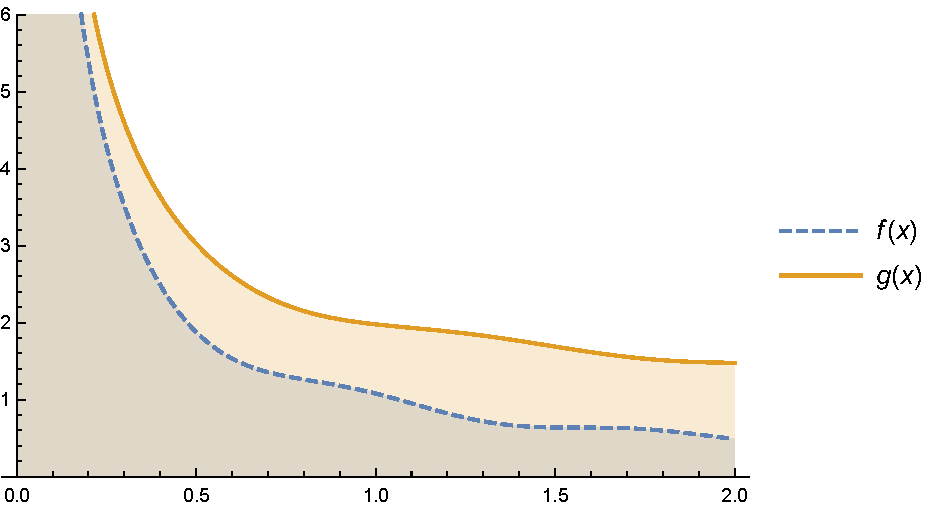
\includegraphics[width=0.5\textwidth]{Figures/improperComp.pdf}
    \caption{Comparing two improper integrals.}
    \label{f:improperintComp}
\end{figure}

\begin{example}\label{e:impintcomp}
    Determine whether the integral $\displaystyle \int_{1}^{\infty} \frac{1}{1+x^{9}}\, dx$ converges.
    
    \begin{solution}
        It's easy to show that for $x \geq 1$ that $0 \leq \frac{1}{1+x^{9}} \leq \frac{1}{x^{9}} \Leftrightarrow 1 + x^{9} \geq x^{9}$. So the integral converges. The actual antiderivative of the function is really messy.
    \end{solution}
\end{example}

\begin{example}\label{e:impintsub}
    Determine if the integral converges or diverges. If it converges, evaluate it: $\displaystyle \int_{-\infty}^{0} \frac{2x}{e^{x^{2}}} \, dx$
    
    \begin{solution}
        \begin{align*}
            \int_{-\infty}^{0} \frac{2x}{e^{x^{2}}} \, dx   &= \lim_{a \to -\infty} \int_{a}^{0} \frac{2x}{e^{x^{2}}} \, dx\\
                                                        &=  -\lim_{a \to \infty} \int_{-a^{2}}^{0} e^{u}\, du \\
                                                        &=  -\lim_{a \to \infty} e^{u} \bigg|_{-a^{2}}^{0}\\
                                                        &= -\lim_{a \to \infty} \left( 1 - \frac{1}{e^{a^{2}}} \right) = -1
        \end{align*}
    \end{solution}
\end{example}

\begin{example}\label{e:impintdiv}
    Determine if the integral $\displaystyle \int_{e}^{\infty} \frac{1}{x\ln x} \, dx$ converges or diverges. If it converges, evaluate it. 
    
    \begin{solution}
        \begin{align*}
            \int_{e}^{\infty} \frac{1}{x\ln x} \, dx    &= \lim_{b \to \infty} \int_{e}^{b} \frac{1}{x\ln x} \, dx\\
                                                        &= \lim_{b \to \infty} \int_{1}^{\ln b} \frac{1}{u} \, du\\
                                                        &= \lim_{b \to \infty} \ln u \Big|_{1}^{\ln b}\\
                                                        &= \lim_{b \to \infty} \left( \ln\left( \ln b \right) \right) = \infty
        \end{align*}
        So the integral diverges.
    \end{solution}
\end{example}

\begin{example}\label{e:impintdouble}
    Determine if the integral $\displaystyle \int_{-\infty}^{\infty} \frac{1}{1 + x^{2}} \, dx$ converges or diverges. If it converges, evaluate it.
    \begin{solution}
        \begin{align*}
            \int_{-\infty}^{\infty} \frac{1}{1 + x^{2}} \, dx   &= \int_{-\infty}^{0} \frac{1}{1 + x^{2}} \, dx + \int_{0}^{\infty} \frac{1}{1 + x^{2}} \, dx \\
                                                                &= \lim_{a \to -\infty} \int_{a}^{0} \frac{1}{1 + x^{2}} \, dx + \lim_{b \to \infty} \int_{0}^{b} \frac{1}{1 + x^{2}} \, dx \\
                                                                &= \lim_{a \to -\infty} \tan^{-1} x \Big|_{a}^{0} + \lim_{b \to \infty} \tan^{-1} x \Big|_{0}^{b}\\
                                                                &= \lim_{a \to -\infty} \left( \tan^{-1} 0 - \tan^{-1} a \right) + \lim_{b \to \infty} \left( \tan^{-1} b - \tan^{-1} 0 \right)\\
                                                                &= \frac{\pi}{2} + \frac{\pi}{2} = \pi
        \end{align*}    
    \end{solution}        
\end{example}

\begin{example}\label{e:impintsub2}
    Determine if the integral converges or diverges. If it converges, evaluate it:
    \[
        \int_{3}^{\infty} \frac{1}{\left( 4x - 1 \right)^{2}} \, dx
    \]    
    \begin{solution}
        \begin{align*}
            \int_{3}^{\infty} \frac{1}{\left( 4x - 1 \right)^{2}} \, dx &= \lim_{b \to \infty} \int_{3}^{b} \frac{1}{\left( 4x - 1 \right)^{2}} \, dx\\
                                                                    &= \frac{1}{4} \lim_{b \to \infty} \int_{11}^{4b - 1} \frac{1}{u^{2}} \, du\\
                                                                    &= -\frac{1}{4} \lim_{b \to \infty} \frac{1}{u}\Big|_{11}^{4b - 1}\\
                                                                    &= -\frac{1}{4} \lim_{b \to \infty} \left( \frac{1}{\left( 4b - 1 \right)^{2}} - \frac{1}{11}\right) \, dx = \frac{1}{44}
        \end{align*}
    \end{solution}
\end{example}

\subsection{Vertical Asymptotes at Limits of Integration}
\begin{itemize}
    \item Basically same idea; function may "pinch" the vertical asymptote "fast enough" to converge
    \item Direction we approach from matters!
    \item Integrals of form $\displaystyle \int_{0}^{b} \frac{1}{x^{p}} \, dx$:
    \begin{align*}
        \int_{0}^{b} \frac{1}{x^{p}} \, dx  &= \lim_{a \to 0^{+}} \int_{a}^{b} \frac{1}{x^{p}} \, dx\\
                                            &= \lim_{a \to 0^{+}} \frac{1}{(p-1)x^{p - 1}}\bigg|_{a}^{b} = \lim_{a \to 0^{+}} \frac{1}{1 - p} \left( \frac{1}{b^{p-1}} - \frac{1}{a^{p-1}} \right)\\
    \intertext{Now we need $p < 1$ for this limit to exist. Assuming this we have}
    \int_{0}^{b} \frac{1}{x^{p}}\, dx  &= \frac{1}{(1 - p)b^{p-1}}
    \end{align*}
    Again, better to work out than memorize.
\end{itemize}

\begin{example}\label{e:impintasymp}
    Determine if the integral converges or diverges. If it converges, evaluate it: $\displaystyle \int_{2}^{4} \frac{1}{\sqrt{8-2x}} \, dx$
    
    \begin{solution}
        \begin{align*}
            \int_{2}^{4} \frac{1}{\sqrt{8-2x}} \, dx    &= \lim_{b \to 4^{-}} \int_{2}^{b} \frac{1}{\sqrt{8-2x}} \, dx\\
                                                        &= -\frac{1}{2} \lim_{b \to 4^{-}} \int_{4}^{8-2b} \frac{1}{\sqrt{u}}\, du\\
                                                        &= -\lim_{b \to 4^{-}} \sqrt{u}\Big|_{4}^{8-2b}\\
                                                        &= -\lim_{b \to 4^{-}} \left( \sqrt{8-2b} - 2 \right) = 2
        \end{align*}
    \end{solution}
\end{example}



\newpage\thispagestyle{firstofchapter}
\chapter{More Applications of Integrals}
\section{Arc Length}
\setcounter{figure}{0}
\begin{itemize}
    \begin{figure}[htbp]
        \centering
            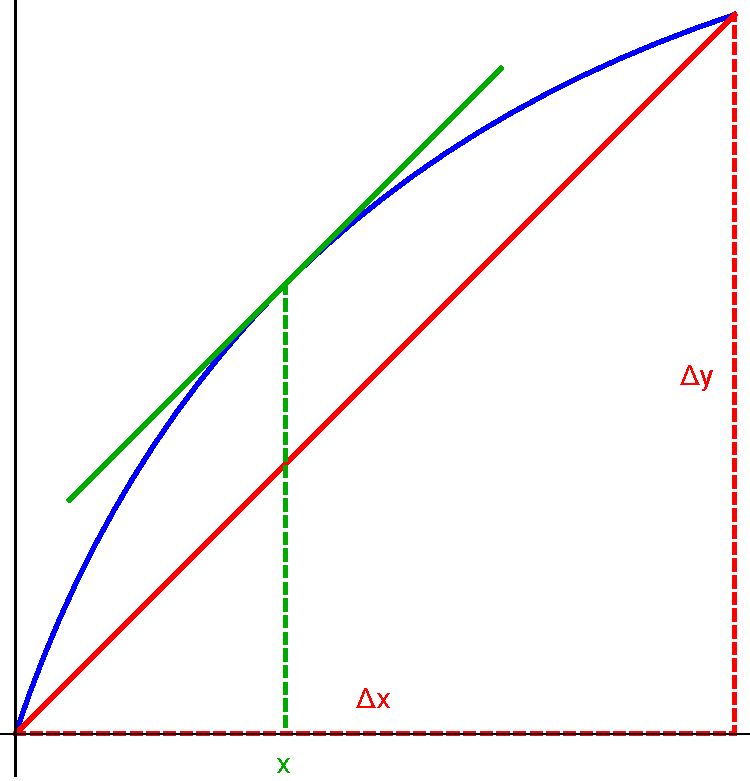
\includegraphics[width=0.25\textwidth]{Figures/arclengthfunc.pdf}
        \caption{Set up arc length integral}
        \label{f:arclengthfunc}
    \end{figure}
    \item Want to find the length along the graph of $y = f(x), a \leq x \leq b$
    \item Use line segments to approximate length of curve
    \item Let $\Delta x$ be the change in $x$, $\Delta y$ the change in $y$ along a segment. Then
    \begin{align*}
        \Delta L    &= \sqrt{(\Delta x)^{2} + (\Delta y)^{2}}\\
                    &= \sqrt{\left(\frac{(\Delta x)^{2}}{(\Delta x)^{2}} + \frac{(\Delta y)^{2}}{(\Delta x)^{2}}\right)(\Delta x)^{2}}\\
                    &= \sqrt{1 + \left(\frac{\Delta y}{\Delta x}\right)^{2}} \Delta x \\
    \end{align*}
    \item $\frac{\Delta y}{\Delta x}$ is the slope of the secant line along this segment
    \item Mean Value Theorem guarantees that there is an $x$ in this interval such that $f'(x) = \frac{\Delta y}{\Delta x}$ giving us
    \[\Delta L = \sqrt{1 + [f'(x)]^{2}} \Delta \]
    \item Do the usual; add them up, take $\Delta x \to 0$ and we get
    \[L = \int_{a}^{b} \sqrt{1 + [f'(x)]^{2}} \, dx\]
    \item In practice these really need to be done with a CAS; some even require different integration techniques
\end{itemize}

\begin{example}\label{e:arc-length-exp}
    Find the length along the graph of $f(x) = \frac{1}{2} \left( e^{x} + e^{-x} \right)$, $-\ln 2 \leq x \leq \ln 2$.
    
    \begin{solution}
        This integrand is a little more complicated:
        \begin{align*}
            f'(x) &= \frac{1}{2}\left( e^{x} - e^{-x} \right)  = \frac{1}{2} e^{x} - \frac{1}{2} e^{-x}        \\
            [f'(x)]^{2} &= \frac{1}{4}e^{2x} - \frac{1}{2} + \frac{1}{4}e^{-x}\\
            1 + [f'(x)]^{2} &= \frac{1}{4}e^{2x} + \frac{1}{2} + \frac{1}{4}e^{-x} = \frac{1}{4} \left( e^{x} + e^{-x} \right)^{2}\\
            \sqrt{1 + [f'(x)]^{2}} &= \frac{1}{2} \left( e^{x} + e^{-x} \right) = f(x) \text{ \faMeh}
        \end{align*}
    
        So the length along the arc is
        \begin{align*}
            L   &= \int_{-\ln 2}^{\ln 2}  \frac{1}{2} \left( e^{x} + e^{-x} \right) \, dx \\
                &= \frac{1}{2}\left( e^{x} - e^{-x} \right)\bigg|_{-\ln 2}^{\ln 2} = \frac{3}{2}
        \end{align*}
        The plot of this part of the curve is in Figure \ref{f:arc-length-exp} but it is not interesting \faMeh
    \end{solution}
    \begin{figure}[htbp]
        \centering
            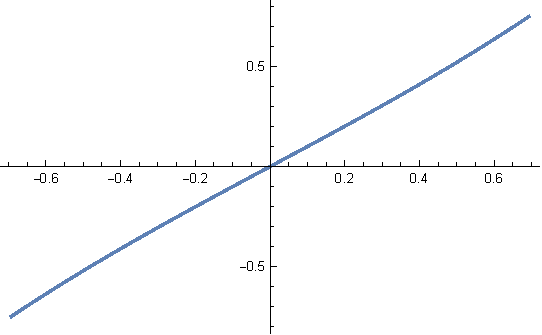
\includegraphics[width=0.4\textwidth]{Figures/arclengthexp.pdf}
        \caption{Plot of function in Example \ref{e:arc-length-exp}}
        \label{f:arc-length-exp}
    \end{figure}    
    \begin{commentary}
        This problem is easier if you recognize $f(x) = \cosh x$ and know the properties $f'(x) = \sinh x$ and $\cosh^{2} x = 1 + \sinh^{2} x$ \faSmile
    \end{commentary}
\end{example}

\begin{example}\label{e:arc-length-lncos}
    \faExclamationCircle[solid] \; This uses the antiderivative of \(\sec x\) and they may not know this depending on text used!

    Find the length along the graph of \(f(x) = \ln (\cos x)\), \(0 \leq x \leq \frac{\pi}{4}\).

    \begin{solution}
        Here \(f'(x) = -\dfrac{\sin x}{\cos x} = -\tan x \Rightarrow \sqrt{1 + [f'(x)]^{2}} = \sqrt{1 + \tan^{2} x} = \sec x\) since \(\sec x\) is positive on \(0 \leq x \leq \frac{\pi}{4}\). So the length is
        \[
            L = \int_{0}^{\pi/4} \sec x \, dx = \ln |\sec x + \tan x|\Big|_{0}^{\pi /4} = \ln (1 + \sqrt{2})
        \]
    The curve is plotted in Figure \ref{f:arc-length-lncos}.
    \end{solution}
    \begin{figure}[htbp]
        \centering
            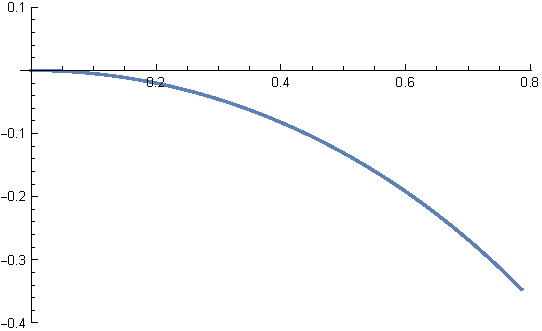
\includegraphics[width=0.4\textwidth]{Figures/arclengthlncos.pdf}
        \caption{Plot of function in Example \ref{e:arc-length-lncos}}
        \label{f:arc-length-lncos}
    \end{figure}
\end{example}

\begin{example}\label{e:trig-sub-arclen}
    Find the length along the graph of $y = x^{2}$, $0 \leq x \leq 1$.
    
    \begin{solution}
        \[L = \int_{0}^{1} \sqrt{1 + 4x^{2}} \, dx \]
        Now we need a substitution first; let $u = 2x \Rightarrow du = 2dx$, $u(0) = 0$, $u(1) = 2$; now we have
        \[\int_{0}^{1} \sqrt{1 + 4x^{2}} \, dx = \frac{1}{2} \int_{0}^{2} \sqrt{1 + u^{2}}\, du\]
        We now make the trig substitution $u = \tan \theta \Rightarrow du \sec^{2} \theta \, d\theta$, $\sqrt{1+u^{2}} = \sec \theta$, $0 = \tan \theta \Rightarrow \theta = 0$, $2 = \tan \theta \Rightarrow \theta = \tan^{-1} 2$:
        \[\frac{1}{2} \int_{0}^{2} \sqrt{1 + u^{2}}\, du = \frac{1}{2} \int_{0}^{\tan^{-1} 2} \sec^{3} \theta \, d\theta\]
        This integral needs integration by parts, but we already did this in Example \ref{e:trigintsec3}. \faSmile \ There we found
        \[\int \sec^{3}\theta \, d\theta = \frac{1}{2}\left(\sec \theta \tan \theta + \ln | \sec \theta + \tan \theta | \right) + C\]
        so now we can just plug away. We will need to use $\tan \theta = 2 \Rightarrow \sec \theta = \sqrt{5}$:
        \begin{align*}
            \frac{1}{2} \int_{0}^{\tan^{-1} 2} \sec^{3} \theta \, d\theta &= \frac{1}{4} \left( \sec \theta \tan \theta + \ln | \sec \theta + \tan \theta | \right)\bigg|_{0}^{\tan^{-1} 2} \\
            &= \frac{\sqrt{5}}{2} + \frac{1}{4}\ln\left( \sqrt{5} + 2 \right)
        \end{align*}
    \end{solution}
\end{example}

\section{Surface Area of Revolution}
\setcounter{figure}{0}
\begin{figure}[htbp]
    \centering
        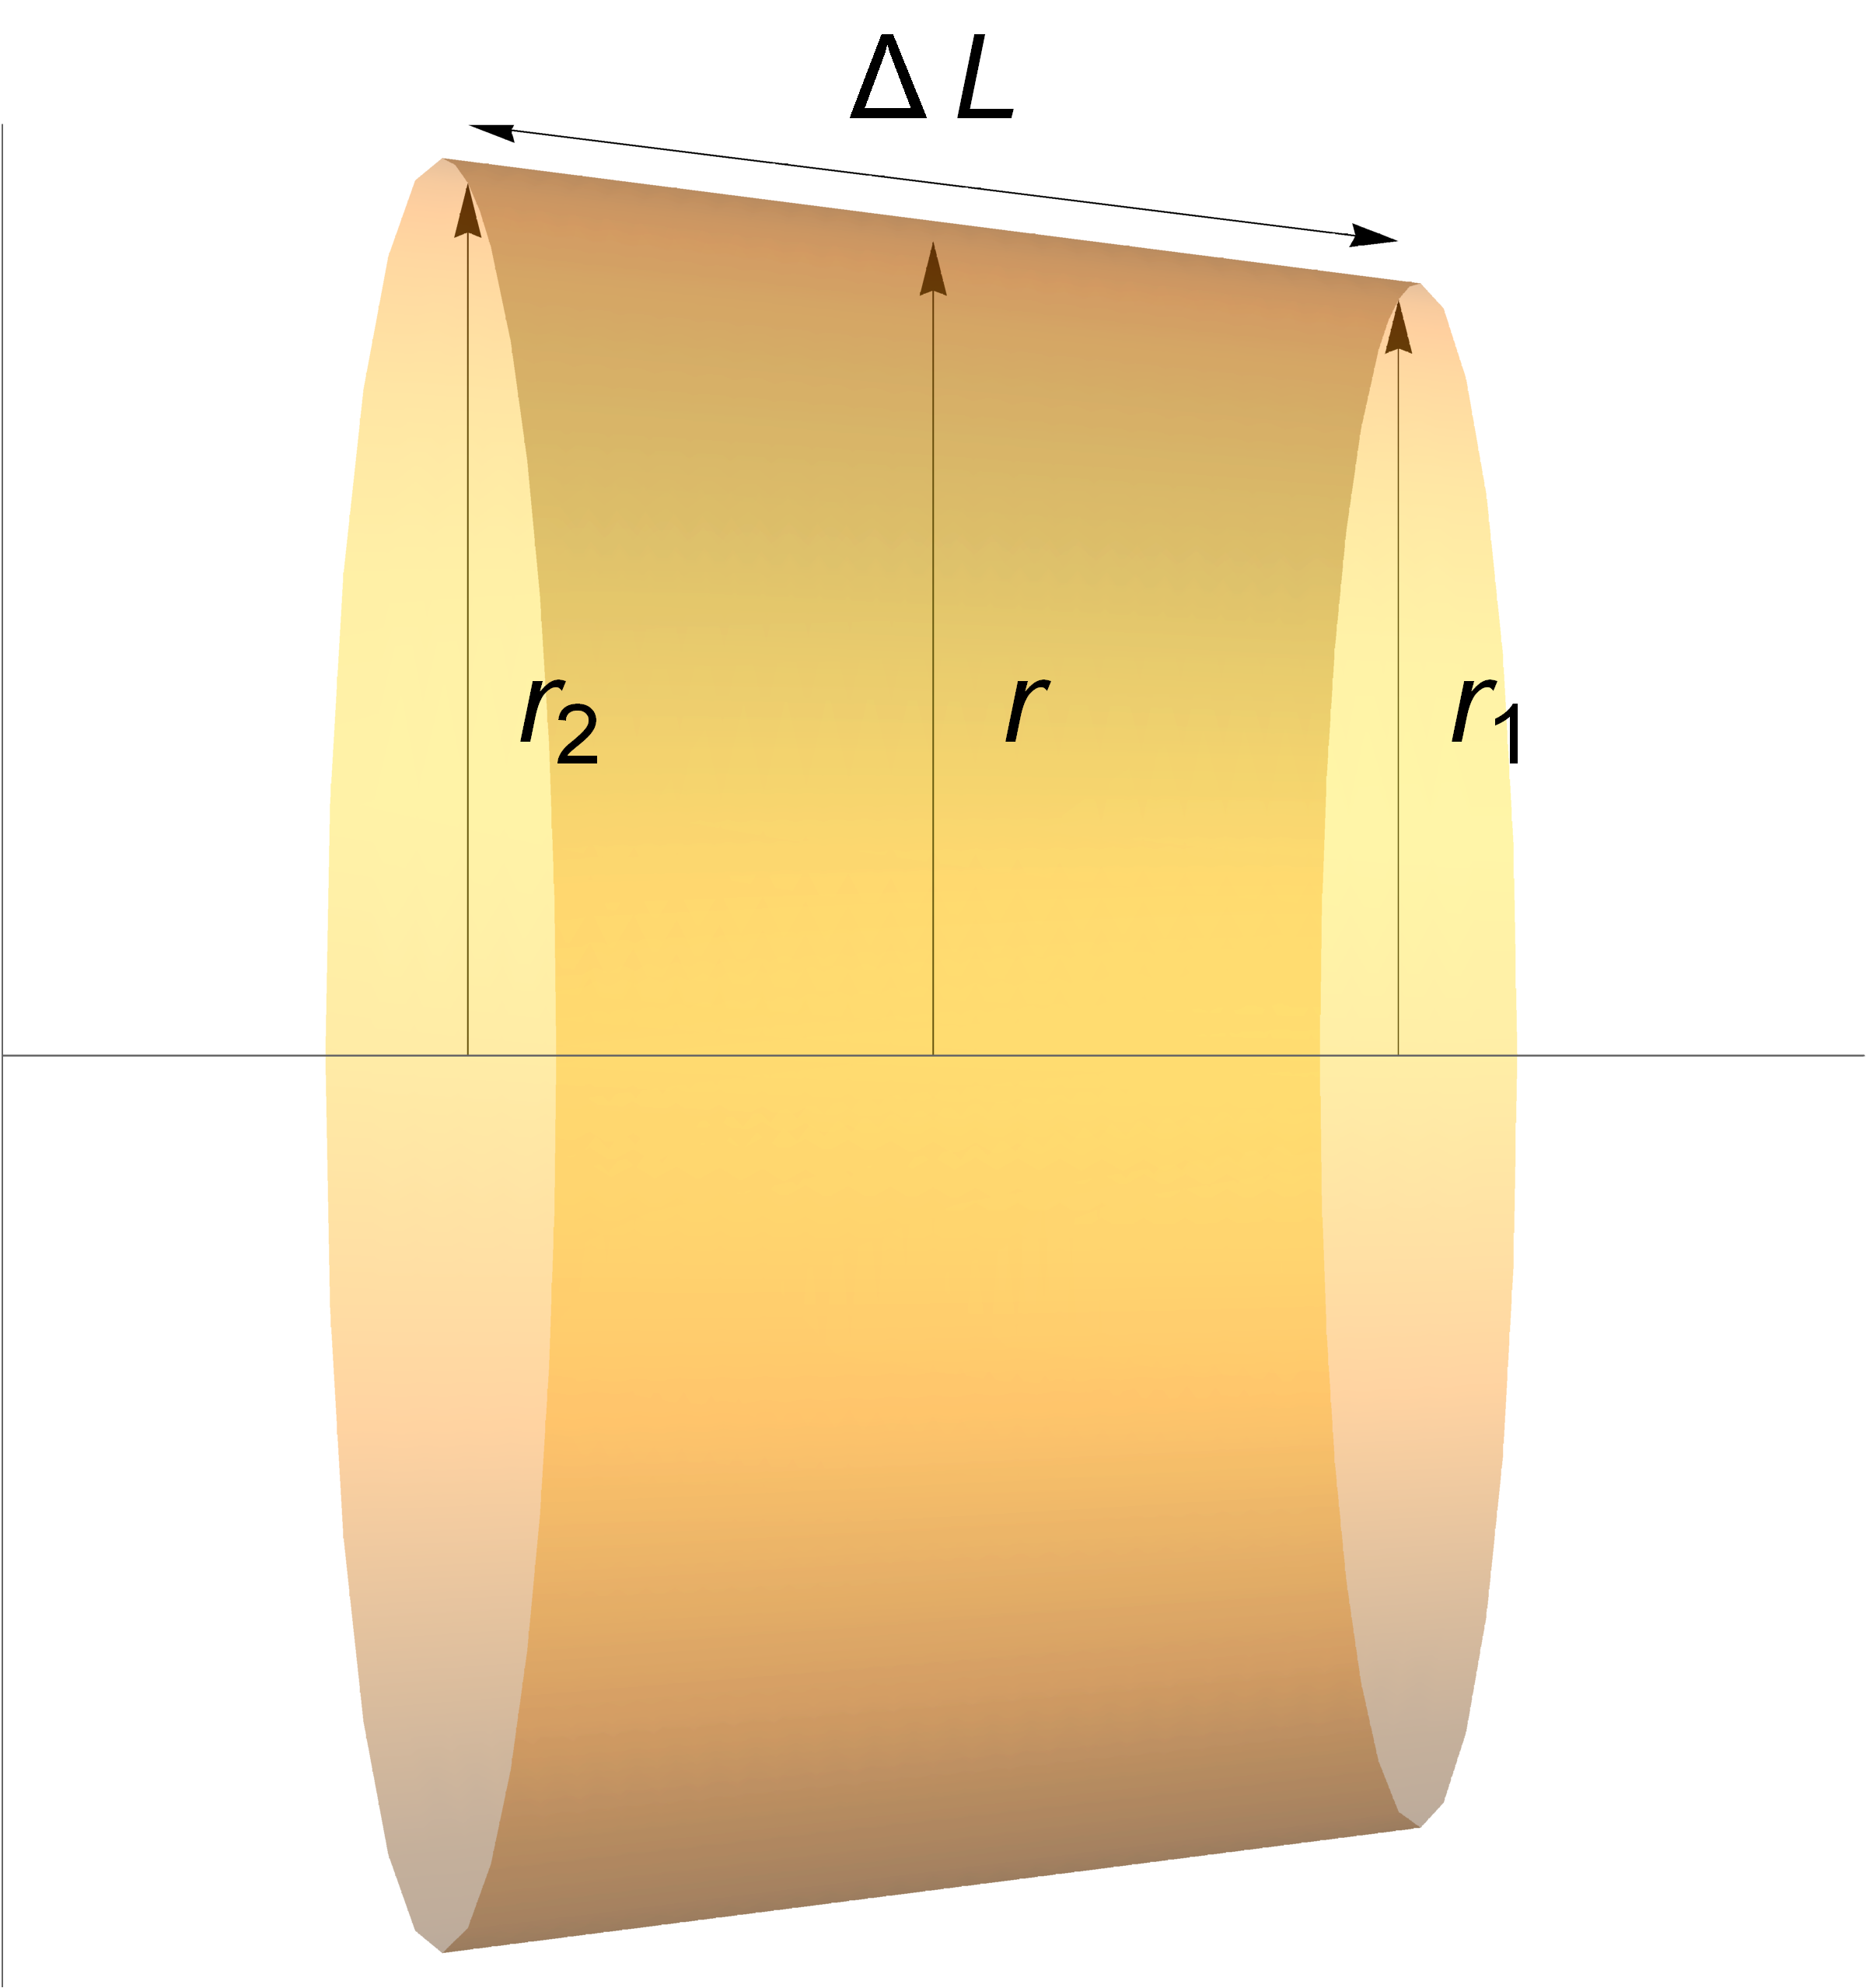
\includegraphics[width=0.25\textwidth]{Figures/surfarearev.png}
    \caption{Frustum of a cone used to approximate surface area of revolution.}
    \label{f:surfarearev}
\end{figure}
\begin{itemize}
    \item Start with revolving $y = f(x)$, $a \leq x \leq b$, about the $x$-axis
    \item Surface area of the frustum of a cone with radii $r_{1} < r_{2}, r = \frac{r_{1} + r_{2}}{2}$ and lateral length $l$: $S = 2\pi r l$
    \item Surface area piece: $\Delta S = 2\pi r \Delta L$
    \item For $r$ we use $f(x)$
    \begin{itemize}
        \item Same $\Delta L$ from arc length!
        \item $\Delta L = \sqrt{1 + [f'(x)]^{2}} \Delta x$
    \end{itemize}
    \item Do the usual adding up area of pieces and take $\Delta x \to 0$ to get the integral:
    \[S = 2\pi \int_{a}^{b} f(x)\sqrt{1 + [f'(x)]^{2}}\, dx\]
    \item If about the $y$-axis, need $x = g(y)$, $c \leq y \leq d$:
    \[S = 2\pi \int_{c}^{d} g(y)\sqrt{1 + [g'(y)]^{2}}\, dy\]
\end{itemize}

\begin{example}
    Find the surface area of revolution formed by taking the graph of $y = x^{3}$, $0 \leq x \leq 1$, about the $x$-axis.
    
    \begin{solution}
        \begin{align*}
            S &= 2 \pi \int_{0}^{1} 9x^{3} \sqrt{1 + 9x^{4}} \, dx
            \intertext{with $u = 1 + 9x^{4}\Rightarrow du = 36x^{2}\, dx, u(0)=1, u(1) = 10$ we get}
            \int_{0}^{1} 9x^{3} \sqrt{1 + 9x^{4}} \, dx &= \frac{\pi}{18} \int_{1}^{10} \sqrt{u}\, du\\
            &= \frac{\pi}{27}\left( 10\sqrt{10} - 1 \right)
        \end{align*}
    \end{solution}
\end{example}

\begin{example}
    Find the surface area of revolution formed by taking the graph of $f(x) = \sqrt{e^{x} + 1}$, $0 \leq x \leq 1$, about the $x$-axis.
    
    \begin{solution}
        First we put together $2\pi f(x) \sqrt{1 + [f'(x)]^{2}}$:
        \begin{align*}
            f'(x) &= \frac{e^{x}}{2\sqrt{e^{x} + 1}}\\
            [f'(x)]^{2} &= \frac{e^{2x}}{4\left( 1 + e^{x} \right)}\\
            1 + [f'(x)]^{2} &= \frac{4\left( 1 + e^{x} \right)}{4\left( 1 + e^{x} \right)} + \frac{e^{2x}}{4\left( 1 + e^{x} \right)}\\
            & = \frac{e^{2x} + 4e^{x} + 4}{4\left( 1 + e^{x} \right)}\\
            &= \frac{(e^{x} + 2)^{2}}{4\left( 1 + e^{x} \right)}\\
            \sqrt{1 + [f'(x)]^{2}} &= \frac{e^{x} + 2}{2\sqrt{e^{x} + 1}}\\
            2\pi f(x) \sqrt{1 + [f'(x)]^{2}} & = 2\pi \sqrt{e^{x} + 1} \cdot \frac{e^{x} + 2}{2\sqrt{e^{x} + 1}} \\
            &= \pi \left( e^{x}  + 2 \right) \text{ \faSmile}
        \end{align*}
        So the surface area is
        \[S = \pi \int_{0}^{1} \left( e^{x}  + 2 \right)\, dx = \pi \left( e + 1 \right)\]
    \end{solution}
\end{example}

\subsection{Volume and Surface Area of Infinite Horn (Optional)}
\begin{itemize}
    \item Make a horn with an infinitely long stem by taking $f(x) = \frac{1}{x}$ on $[1, \infty)$ and rotating about the $x$-axis
    \item Volume of the horn using disks:
    \[V = \pi \int_{1}^{\infty} \left( \frac{1}{x} \right)^{2} \, dx = \pi\]
    \item Surface area of the horn is
    \[S = 2\pi \int_{1}^{\infty} \frac{1}{x} \sqrt{1 + \frac{1}{x^{4}}}\, dx    \]
    This is not a fun antiderivative to find. \faFrown \ But we can do a comparison test by noting that for all $x \geq 1$, $\sqrt{1 + \frac{1}{x^{4}}} > 1$ so $\frac{1}{x} \sqrt{1 + \frac{1}{x^{4}}} > \frac{1}{x}$; but we know that $\displaystyle \int_{1}^{\infty} \frac{1}{x}\, dx$ is divergent, so the surface area integral must be divergent too!
    \begin{itemize}
        \item Side note: the antiderivative is $-2 \sqrt{\frac{1}{x}+1}-\ln \left(1-\sqrt{\frac{1}{x}+1}\right)+\ln
        \left(\sqrt{\frac{1}{x}+1}+1\right)$ \faMeh
    \end{itemize}
    \item So we have a horn with finite volume but infinite surface area!
    \item Seems like a paradox but as usual it really isn't since the "surface" here has zero thickness:
    \begin{itemize}
        \item Volume can be spread over an infinite surface in $\mathbb{R}^{3}$
        \item For example, take a unit cube; slice it into $n$ equally thick slices and you cover $n$ square units of area
        \item As $n \to \infty$, $S \to \infty$
    \end{itemize}
\end{itemize}


\newpage\thispagestyle{firstofchapter}
\chapter{Sequences and Series}
\setcounter{figure}{0}
\section{Sequences}
\begin{itemize}
    \item A \textbf{sequence} is a function $a_{n}: \mathbb{N} \rightarrow \mathbb{R}$; usually $a_{n} = f(n)$
    \item Less formally, a sequence is an infinite ordered list of real numbers
    \item Notation: $\left\{a_{n}\right\}_{n=1}^{\infty} = a_{1}, a_{2}, a_{3}, \ldots$
    \item Can leave off limits usually
    \item Can be defined recursively (in terms of previous terms)
    \begin{itemize}
        \item Fibonacci Sequence: $f_{1} = 1, f_{2} = 1$; $f_{n} = f_{n-1} + f_{n-2}$ for $n \geq 3$
    \end{itemize}
    \item \textbf{Limit} of a sequence
    \begin{itemize}
        \item $\displaystyle \lim_{n \to \infty} a_{n} = L$ means we can make $a_{n}$ as close as we want to $L$ by making $n$ a large enough positive integer
        \item Most all limit laws from Calc I apply except, technically, L'Hospital's Rule (but we can work around this)
        \item If $\displaystyle \lim_{x \to \infty} f(x) = L$ and $ \forall n \in \mathbb{N}, f(n) = a_{n}$ then $\lim_{n \to \infty} a_{n} = L$.
        \item If limit exists, \textbf{convergent}. Else \textbf{divergent}.
        \item Note that $\displaystyle \lim_{n \to \infty} |a_{n}| = 0 \Rightarrow \lim_{n \to \infty} a_{n} = 0$.
        \item Can often use the dominant terms method
    \end{itemize}    
\end{itemize}

\begin{example}\label{e:seqalt}
    Determine if the following sequences converges or diverges: $\displaystyle \left\{ \frac{(-1)^{n}(2n+3)}{4n^{2}-1}\right\}_{n = 1}^{\infty}$
    
    \begin{solution}
        \[\lim_{n \to \infty} \left| \frac{(-1)^{n}(2n+3)}{4n^{2}-1} \right| = \lim_{n \to \infty} \frac{2n+3}{4n^{2}-1} = 0\]
        and the sequence converges to 0.
    \end{solution}
\end{example}

\begin{example}\label{e:seq-alternating-limit}
    Determine if the following sequences converges or diverges: \(\displaystyle \left\{ \frac{(-1)^{n}(3n+2)}{n+1}\right\}_{n = 1}^{\infty}\)
    \begin{solution}
        Note that the alternating factor \((-1)^{n}\) does not affect the magnitude of the expression, just the sign. The non-alternating part has \(\displaystyle \lim_{n\to \infty} \frac{3n+2}{n+1} = 3\), so as \(n\to \infty\) the expression is alternating between values very close to \(\pm 2\) but do not settle down on one value. So this limit does not exist.
    \end{solution}
\end{example}

\begin{example}\label{e:seqexp}
    Determine if the following sequences converges or diverges: $\displaystyle \left\{ \frac{2^{n}}{3^{n} + 1} \right\}_{n = 0}^{\infty}$
    
    \begin{solution}
        \[\lim_{n \to \infty}\frac{2^{n}}{3^{n} + 1} = \lim_{n \to \infty}\frac{\frac{2^{n}}{3^{n}}}{1 + \frac{1}{3^{n}}} = 0\]
        and the sequence converges.
    \end{solution}
\end{example}

\begin{itemize}
    \item $n! = n(n-1)(n-2)\cdots (2)(1)$, $n \geq 1$
    \item $0! = 1$ by definition
\end{itemize}

\begin{example}\label{e:seqfac}
    Determine if the following sequences converges or diverges: $\displaystyle \left\{ \frac{n!}{n^{n}} \right\}_{n = 0}^{\infty}$
    
    \begin{solution}
        Note that
        \[0 < \frac{n!}{n^{n}} = \frac{1\cdot 2 \cdots n}{n \cdot n \cdots n} < \frac{1}{n}\]
        so by the Squeeze Theorem, $\displaystyle \lim_{n \to \infty}\frac{n!}{n^{n}} = 0$.
    \end{solution}
\end{example}

\begin{itemize}
    \item A sequence $\left\{a_{n}\right\}$ is \textbf{bounded above} if $\exists M, a_{n} \leq M\; \forall n\in \mathbb{N}$
    \item A sequence $\left\{a_{n}\right\}$ is \textbf{bounded below} if $\exists m, m \leq a_{n}\; \forall n\in \mathbb{N}$
    \item A sequence is \textbf{bounded} if it is bounded above and below
    \item A sequence is \textbf{monotonic} if it is either non-increasing or non-decreasing
    \item Sequences that are bounded and monotonic are convergent.
    \begin{itemize}
        \item Proof uses Completeness Axiom
        \item Every subset of $\mathbb{R}$ that is bounded above has a least upper bound, the \textbf{supremum} of the set
    \end{itemize}
\end{itemize}

\section{Series}
\setcounter{figure}{0}
\begin{itemize}
    \item A \textbf{series} is the sum over a sequence:
    \[\sum_{n=1}^{\infty} a_{n} = a_{1} + a_{2} + a_{3} + \cdots\]
    \item The $n$\textsuperscript{th} partial sum, $s_{n}$, is the sum of the first $n$ terms of the series:
    \[s_{n} = \sum_{k=1}^{n} a_{k}\]
    \item If $\displaystyle \lim_{n \to \infty} s_{n} = S$ where $S$ is a real number, we say the series \textbf{converges} and its sum is $S$. If this limit does not exist we say the series \textbf{diverges}.
    \item If a series converges, then $\displaystyle \displaystyle \lim_{n \to \infty} a_{n} = 0$.
    \begin{itemize}
        \item[{\faExclamationTriangle[solid]}] Note that the converse is not true in general!
    \end{itemize}
    \item Even better: if $\displaystyle \lim_{n \to \infty} a_{n} \neq 0$, then $\sum a_{n}$ diverges.
    \item Properties of convergent series:
    \begin{itemize}
        \item $\displaystyle \sum c a_{n} = c \sum a_{n}$
        \item $\displaystyle \sum (a_{n} + b_{n}) = \sum a_{n} + \sum b_{n}$
    \end{itemize}
    \item[{\faExclamationCircle[solid]}] Note that we do not care about the first finitely many terms of a series, i.e. $\displaystyle \sum_{n = 1}^{\infty} a_{n}$ converges iff $\displaystyle \sum_{n = k}^{\infty} a_{n}$ converges.
\end{itemize}

\begin{example}\label{e:seriesexp}
    Determine if the series $\displaystyle \sum_{n=1}^{\infty} \frac{1}{2^{n}}$ converges or diverges. If it converges, find its sum.
    
    \begin{solution}
        In general, $\displaystyle s_{n} = \frac{2^{n} - 1}{2^{n}}$; $\displaystyle \lim_{n \to \infty} \frac{2^{n} - 1}{2^{n}} = 1$ So the series is convergent and the sum is 1.
    \end{solution}
\end{example}

\begin{example}\label{e:seriestelsum}
    Determine if the series $\displaystyle \sum_{n=1}^{\infty} \left( \frac{1}{n} - \frac{1}{n+1} \right)$ converges or diverges. If it converges, find its sum.
    
    \begin{solution}
        This is a telescoping sum. Note that
        \begin{align*}
            s_{n}   &= \left( 1 - \frac{1}{2} \right) + \left( \frac{1}{2} - \frac{1}{3} \right) + \left( \frac{1}{3} - \frac{1}{4} \right) + \cdots +  \left( \frac{1}{n-1} - \frac{1}{n} \right) + \left( \frac{1}{n} - \frac{1}{n+1} \right)\\
                    &= 1 - \frac{1}{n+1}
        \end{align*}
        And then we have $\displaystyle \lim_{n \to \infty} \left( 1 -  \frac{1}{n+1}\right) = 1$ so the series is convergent and the sum is 1.
    \end{solution}
\end{example}

\subsection{Geometric Series}
\begin{itemize}
    \item A \textbf{geometric series} has the form
    \[\sum_{n=0}^{\infty} a r^{n} = a + ar + ar^{2} + ar^{3} + \cdots\]
    \item Converges iff $|r| < 1$:
    \begin{alignat*}{5}
        &s_{n}          & &= a {}&{}+{}  &ar {}+{} ar^{2} + \cdots + ar^{n-1} &{}\\
        -r&s_{n}        & &=     {}&{}-{}&ar {}-{} ar^{2} - \cdots              &-ar^{n}\\
        s_{n} - r&s_{n} & &= a &{}&{} &-ar^{n}
    \end{alignat*}
    So $s_{n}(1-r) = a - ar^{n} \Rightarrow s_{n} = \frac{a(1-r^{n})}{1-r}$. If  $|r| < 1$ then as $n \to \infty, r^{n} \to 0$ and we have
    \[S = \lim_{n \to \infty} \frac{a(1-r^{n})}{1-r} = \frac{a}{1 - r}\]
    The limit does not exist if $|r| \geq 1$.
\end{itemize}

\begin{example}\label{e:seriesgeo}
    Determine if the series $\displaystyle \sum_{n=0}^{\infty} 3 \left( \frac{2}{5} \right)^{n}$ converges or diverges. If it converges, find its sum.
    
    \begin{solution}
        Here $r = \frac{2}{5}$ so the series converges and $S = \frac{3}{1 - \frac{2}{5}} = 5$.
    \end{solution}
\end{example}

\begin{example}\label{e:seriesgeoconv}
    Determine if the series $\displaystyle \sum_{n=1}^{\infty} 2\left( -\frac{3}{4} \right)^{n}$ converges or diverges. If it converges, find its sum.
    
    \begin{solution}
        Not quite geometric! Starts at $n=1$! But $r = -\frac{3}{4}$ so the series converges. The first "few" terms of a series don't matter with convergence. The "full" series starting with $n=0$ has the sum $\frac{2}{1 + \frac{3}{4}} = \frac{8}{7}$ so we can just subtract the $n=0$ term to get
        \[\sum_{n=1}^{\infty} 2\left( -\frac{3}{4} \right)^{n} = \sum_{n=0}^{\infty} 2\left( -\frac{3}{4} \right)^{n} - 2 = -\frac{6}{7}\]
    \end{solution}
\end{example}

\begin{example}\label{e:seriesGrandis}
    Determine if the series $\displaystyle \sum_{n=0}^{\infty} \left( -1 \right)^{n}$ converges or diverges. If it converges, find its sum.
    
    \begin{solution}
        The terms of this series just toggle from 1 to $-1$. The limit of the terms is not 0, so the series diverges (\textit{and don't let anybody tell you different}). Note also $r=-1$.
    \end{solution}
\end{example}

\begin{example}\label{e:seriesxvals}
    For what values of $x$ does the series $\displaystyle \sum_{n=0}^{\infty} \left( 2(x-3) \right)^{n}$ converge?
    
    \begin{solution}
        We need $|2(x-3)| < 1 \Rightarrow \frac{5}{2} < x < \frac{7}{2}$.
    \end{solution}
\end{example}

\begin{example}\label{e:seriesdectofrac}
    Write $0.\overline{64} = 0.64646464\ldots$ as an exact fraction.
    
    \begin{solution}
        \begin{align*}
            0.\overline{64} &= \frac{64}{100} + \frac{64}{10000} + \frac{64}{1000000} + \cdots \\
                            &= \frac{64}{100} \left( 1 + \frac{1}{100} + \frac{1}{10000} + \cdots \right)\\
                            &= \frac{64}{100} \left( 1 + \frac{1}{100} + \left( \frac{1}{100} \right)^{2} + \cdots \right) \\
                            &= \frac{64}{100} \sum_{n=0}^{\infty} \left( \frac{1}{100} \right)^{n}\\
                            &= \frac{64}{100} \cdot \frac{1}{1-\frac{1}{100}} = \frac{64}{99}
        \end{align*}
    \end{solution}
\end{example}

\begin{example}\label{e:seriesdectofrac1}
    Write $0.\overline{9} = 0.99999\ldots$ as an exact fraction.
    
    \begin{solution}
        \begin{align*}
            0.\overline{9}  &= \frac{9}{10} + \frac{9}{100} + \frac{9}{1000} + \frac{9}{10000} + \frac{9}{100000} + \cdots\\
                            &= \frac{9}{10} \left( 1 + \frac{1}{10} + \frac{1}{100} + \frac{1}{1000} + \frac{1}{10000} + \cdots \right)\\
                            &= \frac{9}{10} \sum_{n=0}^{\infty} \left( \frac{1}{10} \right)^{n}\\
                            &= \frac{9}{10} \cdot \frac{10}{9} = 1 \text{ \faSmile}
         \end{align*}
         This does not seem right since $0.\overline{9}$ looks like it is less than 1 but it's equal to 1! If $0.\overline{9} \neq 1$ then there is a real number in between them. What could its decimal representation be? \faSmile
    \end{solution}
\end{example}

\begin{example}\label{e:seriesKochcurve}
    The \textbf{Koch snowflake curve} is made by:
    \begin{enumerate}
        \item Start with an equilateral triangle
        \item Divide each side into three segments of equal length
        \item Use middle segment as base of equilateral triangle pointing out
        \item Remove base of the new triangle
        \item Go to step 2
    \end{enumerate}
    This repeats ad infinitum and creates a fractal curve. The first few iterations of the curve is show in Figure \ref{f:snowflakes}.
    \begin{figure}[htbp]
        \centering
            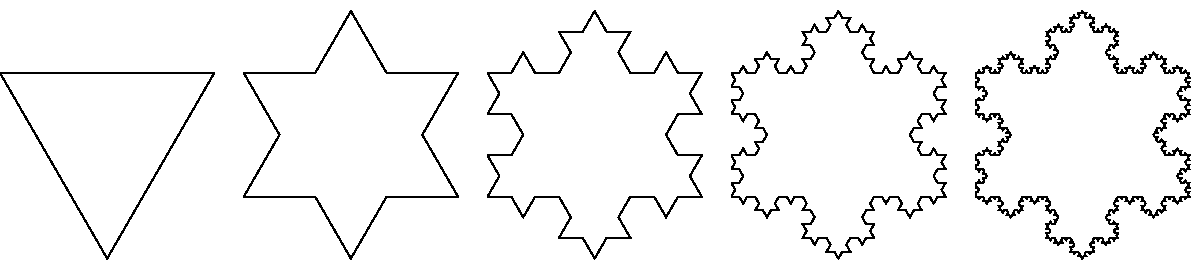
\includegraphics[width=\textwidth]{Figures/snowflaskes.pdf}
        \caption{First four iterations of the snowflake curve.}
        \label{f:snowflakes}
    \end{figure}
    \begin{enumerate}
        \item Find the area of the snowflake curve if we start with an equilateral triangle with side length 1.        
        
        \begin{solution}
            \begin{itemize}
                \item The starting triangle has a base of 1 and a height of $\frac{\sqrt{3}}{2}$ so the starting area is $a_{0} = \frac{1}{2}\cdot 1 \cdot \frac{\sqrt{3}}{2} = \cdot \frac{\sqrt{3}}{4}$
                \item On each iteration, each existing side adds a new triangle in the middle third; we start with \(S_{0} = 3\) sides; after \(n\) iterations we have \(S_{n} = 3 \cdot 4^{n}\) sides
                \item The number of new triangles we add on the \(n\)\textsuperscript{th} iteration is \(t_{n} = S_{n-1} = 3\cdot 4^{n-1}\)
                \item Each new triangle added after $n$ iterations has an area of $a_{n} = \frac{1}{9}a_{n-1} = \frac{\sqrt{3}}{4} \cdot \frac{1}{9^{n}}$
                \item The total new area after $n$ iterations is
                \[A_{n} = a_{n} t_{n} = \frac{\sqrt{3}}{4}\cdot \frac{1}{9^{n}} \cdot 3 \cdot 4^{n-1} = \frac{\sqrt{3}}{4} \cdot \frac{3}{4}\left( \frac{4}{9} \right)^{n}\]
                \item The total area of the curve then is
                \begin{align*}
                    A   &= A_{0} + \sum_{n=1}^{\infty} A_{n} = \frac{\sqrt{3}}{4} + \frac{\sqrt{3}}{4} \sum_{n=1}^{\infty} \frac{3}{4}\left(\frac{4}{9} \right)^{n}\\
                        &= \frac{\sqrt{3}}{4} \left( 1 +  \sum_{n=1}^{\infty} \frac{3}{4}\left( \frac{4}{9} \right)^{n} \right) = \frac{\sqrt{3}}{4} \left( 1 + \frac{3}{4}\sum_{n=0}^{\infty} \left( \frac{4}{9} \right)^{n+1} \right)\\
                        &= \frac{\sqrt{3}}{4} \left( 1 + \frac{1}{3}\sum_{n=0}^{\infty} \left( \frac{4}{9} \right)^{n} \right) = \frac{\sqrt{3}}{4} \left( 1 + \frac{3}{5} \right) = \frac{2\sqrt{3}}{5}
                \end{align*}
            \end{itemize}
        \end{solution}
        
        \item Find the perimeter of the snowflake curve.        
        
        \begin{solution}
            The number of sides after $n$ iterations is $S_{n} = 3 \cdot 4^{n-1}$ and each side has length $l_{n}=\left( \frac{1}{3} \right)^{n-1}$. So the perimeter is
            \[P = \lim_{n\to\infty} S_{n} l_{n} = \lim_{n\to\infty} 3\cdot \left( \frac{4}{3} \right)^{n-1} = \infty\]
        \end{solution}
    \end{enumerate}

The curve has a finite area and an infinite perimeter! Further, there are no tangent lines to the curve!
\end{example}

\begin{itemize}
    \item For the most part finding the sum of a convergent series is difficult
    \item There are some series we do not even know whether or not they are convergent!
    \begin{itemize}
        \item $\displaystyle \sum_{n=1}^{\infty} \frac{1}{n^{3} \sin^{2} n}$; none of our tests will work \faFrown
    \end{itemize}
\end{itemize}

\section{The Integral Test}
\setcounter{figure}{0}

\begin{itemize}
    \item From now on we are just going to see if a series converges or diverges
    \item If $f$ is continuous, positive, and decreasing when $x \geq 1$ and $a_{n} = f(n)$ when $n \in \mathbb{N}$ then the \textbf{integral test} states that
    \[\sum_{n=1}^{\infty} a_{n} \text{ converges} \Leftrightarrow \int_{1}^{\infty} f(x) \, dx \text{ converges}\]
    Illustrations as to why are given in Figures \ref{f:inttestconv} and \ref{f:inttestdiv}.
    \item Basic idea: if there is finite area under the curve, finite area in boxes; infinite area under curve, infinite area in boxes
    \item[{\faExclamationCircle[solid]}] This test is usually toughest and usually there are better tests
    \item Not too many situations where this is the best test to use
    \item [{\faExclamationTriangle[solid]}] If the integral converges, its value is not necessarily (really, almost never) the sum of the series
\end{itemize}

\begin{figure}[htbp]%
    \centering
    \begin{minipage}{0.45\textwidth}%
        \centering
        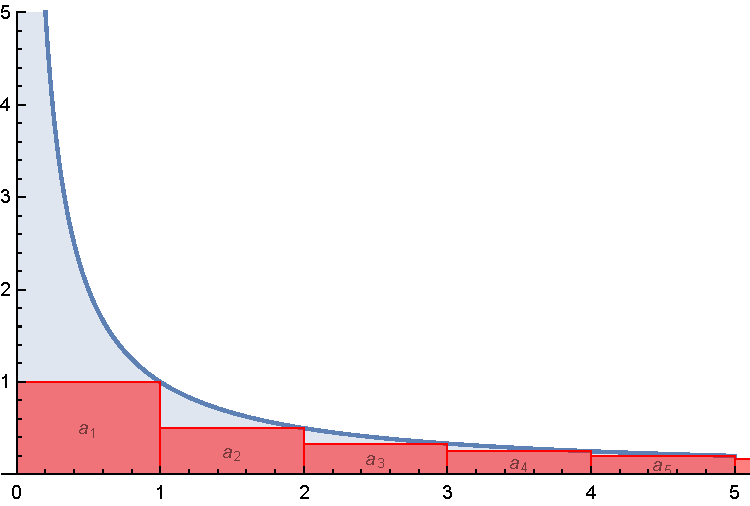
\includegraphics[width=0.9\textwidth]{Figures/inttestconv.pdf}%
        \caption{Sum of series versus value of integral when both converge}%
        \label{f:inttestconv}
    \end{minipage}\hfill
    \begin{minipage}{0.45\textwidth}%
        \centering
        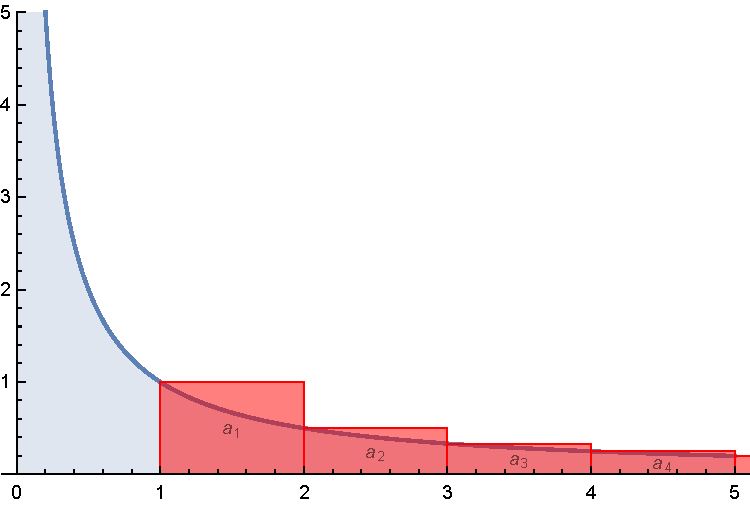
\includegraphics[width=0.9\textwidth]{Figures/inttestdiv.pdf}%
        \caption{Sum of series versus value of integral when both diverge}%
        \label{f:inttestdiv}
    \end{minipage}\hfill
\end{figure}

\begin{example}\label{e:seriesinttestpseries}
    Determine the values of $p$ for which the series  $\displaystyle \sum_{n=1}^{\infty} \frac{1}{n^{p}}$ converges.
    
    \begin{solution}
        This is a $\bm{p}$\textbf{-series} and we already got this. This is just what we had back in Improper Integrals. This series will converge when $p>1$ and diverge when $p \leq 1$.
        Some particular examples:
        \begin{itemize}
            \item $\displaystyle \sum_{n=1}^{\infty} \frac{1}{n}$ diverges. This is known as the \textbf{harmonic series}.
            \item $\displaystyle \sum_{n=1}^{\infty} \frac{1}{n^{2}} = \frac{\pi^{2}}{6}$; this was the Basel Problem and we will see a proof of this later
            \item $\displaystyle \sum_{n=1}^{\infty} \frac{1}{n^{4}} = \frac{\pi^{4}}{90}$
            \item Nobody knows exactly what $\displaystyle \sum_{n=1}^{\infty} \frac{1}{n^{3}}$ converges to \ \faFrown \ We can use various methods to estimate convergent series, though, and this is about equal to 1.20206.
        \end{itemize}
    \end{solution}
\end{example}

\begin{example}\label{e:seriesinttest2}
    Determine whether the series $\displaystyle \sum_{n=1}^{\infty} \frac{2n}{n^{4} + 1}$ converges or diverges.
    
    \begin{solution}
        While we'll see a better test for this later, we will use the convergence of the series here for something else. First, make sure this series meets the conditions. All terms are positive. Is it decreasing? It might be easier to show that for $\displaystyle f(x) = \frac{2x}{x^{4} + 1}$ that $f'(x)<0$ when $x \geq 1$.
        \[f'(x) =  \frac{2-6 x^4}{\left(x^4+1\right)^2} \Rightarrow f'(x) < 0 \text{ when } x \geq \frac{1}{\sqrt[4]{3}} \text{ \faSmile}\]
        So it meets the conditions. But now we still need to perform the test! \ \faMeh
        \begin{align*}
            \int_{1}^{\infty} \frac{2x}{x^{4} + 1} \, dx                &= \lim_{b \to \infty} \int_{1}^{b} \frac{2x}{x^{4} + 1} \, dx
            \intertext{With $u = x^{2} \Rightarrow du = 2x\, dx$, $u(b) = b^{2}, u(1) = 1$ we get}
            \lim_{b \to \infty} \int_{1}^{b} \frac{2x}{x^{4} + 1} \, dx &= \lim_{b \to \infty} \int_{1}^{b^{2}} \frac{1}{u^{2} + 1} \, du\\
                                                                        &= \lim_{b \to \infty} \tan^{-1} u \Big|_{1}^{b^{2}}\\
                                                                        &= \lim_{b \to \infty} \left( \tan^{-1} b^{2} - \frac{\pi}{4} \right)\\
                                                                        &= \frac{\pi}{2}- \frac{\pi}{4} = \frac{\pi}{4}
        \end{align*}
        so the series converges.
    \end{solution}
\end{example}

\subsection{Estimating Sums}
\begin{itemize}
    \item[{\faExclamationCircle[solid]}] Much of this requires a calculator/CAS
    \item Sometimes cannot find sum or it is too messy to be helpful
    \item Use partial sums to estimate sum of series
    \item How close are we to the sum of the full series by using $s_{n}$?
    \item If $\displaystyle \sum a_{n} = S$ converges, let the $\bm{n}$\textbf{\textsuperscript{th} Remainder} be $R_{n} = S - s_{n} = a_{n + 1} + a_{n + 2} + \cdots$
    \item We will get upper bounds on $R_{n}$
    \item For integral test, we have $\displaystyle \int_{n+1}^{\infty} f(x) \, dx \leq R_{n} \leq \int_{n}^{\infty} f(x) \, dx$ (see Figure below)
\end{itemize}

\begin{figure}[htbp]
    \centering
    \begin{minipage}{0.45\textwidth}
        \centering
        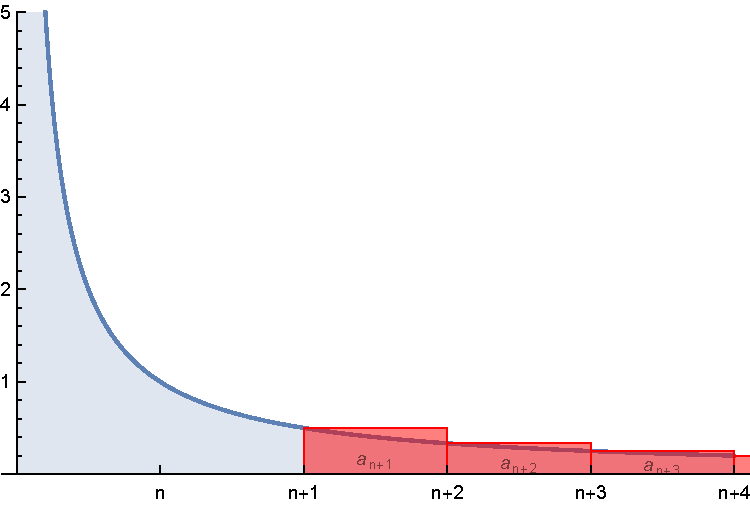
\includegraphics[width=0.9\textwidth]{Figures/intttestremainderlb.pdf}
        \caption{Lower bound on remainder.}
        \label{f:intttestremainderlb}
    \end{minipage}\hfill
    \begin{minipage}{0.45\textwidth}
        \centering
        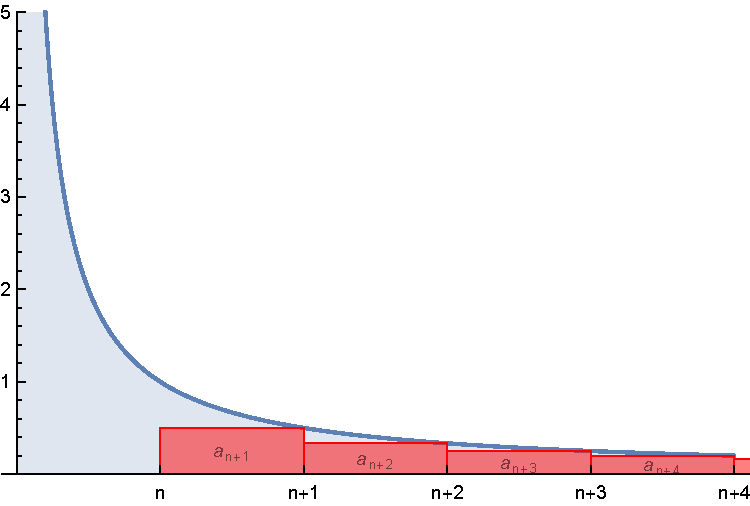
\includegraphics[width=0.9\textwidth]{Figures/intttestremainderub.pdf}
        \caption{Upper bound on remainder.}
        \label{f:intttestremainderub}
    \end{minipage}\hfill
\end{figure}

\begin{example}\label{e:seriesinttestestsum}
    \begin{enumerate}
        \item Find an upper bound on the error in using $s_{10}$ to approximate $\displaystyle \sum_{n=1}^{\infty} \frac{2n}{n^{4} + 1}$.
        \item How many terms are needed to ensure that \(R_n < 0.0005\)? 
    \end{enumerate}     
   
   \begin{solution}
    \begin{enumerate}
        \item  We already did most of the work here, fortunately; we have $\displaystyle R_{n} \leq \int_{n}^{\infty} \frac{2x}{x^{4} + 1} \, dx = \frac{\pi}{2} - \tan^{-1} n^{2}$ so we have the upper bound $R_{10} \leq \frac{\pi}{2} - \tan^{-1} 100 \approx 0.00999967$.
    
        $s_{10} \approx 1.37929645$; according to Mathematica the sum of the entire series to 8 decimal places is $S \approx 1.38834604$, so $R_{10} \approx 0.00904959$. So it did indeed come within the upper bound but not by much!

        \item We need to solve \(\frac{\pi}{2} - \tan^{-1} n^{2} < 0.0005\) which requires a CAS; per Mathematica, we need \(n \geq 45\) terms. \faMeh \ Here \(s_{45} \approx 1.38786\) so with rounding it does get the sum correct to three decimal places, and \(R_{45} \approx 0.00048\).
    \end{enumerate}     
   \end{solution}
\end{example}

\subsection{Removing Terms from Divergent Series (Optional)}
\begin{itemize}
    \item We already know $\displaystyle \sum_{n=1}^{\infty} \frac{1}{n}$ diverges
    \item But what if we remove all of the terms where the digit 9 appears in the denominator?
    \item Suppose $n$ has $d$ digits. There are $9 \cdot 10^{d-1}$ $d$-digit numbers. Of those, $8 \cdot 9^{d-1}$ do not have a 9. If \(n\) has \(d\) digits, \(n \geq 10^{d-1} \Rightarrow \frac{1}{n} \leq \frac{1}{10^{d-1}}\).
    \item So the sum of reciprocals all $d$-digit numbers with no 9 is at most $8\cdot \left( \frac{9}{10} \right)^{d-1}$
    \item Summing over $d$ we get the sum of all of these reciprocals is at most
    \[8 \sum_{d=1}^{\infty} \left( \frac{9}{10} \right)^{d-1} = \frac{8}{1 - \frac{9}{10}} = 80\]
    \item Of course the sum is greater than 0 so the partial sums are bounded; further the partial sums are monotonic so they are convergent! Removing all of the terms with a 9 made what was a divergent series converge!
    \item Exact value of this series is not known but is approximately 22.921
    \item The "Frivolous Theorem of the Natural Numbers" states that most natural numbers are \textit{really} large \faSmile
    \item But if $n$ is very large, it's very unlikely that it does not have every digit
    \item The proportion of $d$-digit numbers with no 9 is
    \[\frac{8 \cdot 9^{d-1}}{9 \cdot 10^{d-1}} = \frac{8}{9} \left( \frac{9}{10} \right)^{d-1}\]
    \item Note that as $d \to \infty$, $\left( \frac{9}{10} \right)^{d-1} \to 0$
\end{itemize}

\section{Comparison Tests}
\setcounter{figure}{0}
\begin{itemize}
    \item We can use other known series to compare against others like we did for improper integrals
    \item Still need all positive terms
\end{itemize}

\subsection{Direct Comparison Test}
\begin{itemize}
    \item This one is less desirable but sometimes necessary \faMeh
    \item Suppose that $0 < a_{n} \leq b_{n}$ for all $n \in \mathbb{N}$. Then:
    \begin{itemize}
        \item If $\sum a_{n}$ diverges, so does $\sum b_{n}$.
        \item If $\sum b_{n}$ converges, so does $\sum a_{n}$.
    \end{itemize}
    \item[{\faExclamationTriangle[solid]}] Must establish the inequality $0 < a_{n} \leq b_{n}$ for all $n$ in index range of the series in your work!
    \item[{\faExclamationTriangle[solid]}] If you cannot show this inequality you cannot use this test! 
    \item Basic idea is that one series will either "lift up" or "squish down" the other
    \item This is much better than the Integral Test but still not as good as most in most cases
    \item For rational terms take the dominant terms to make a comparison series
\end{itemize}

\begin{example}\label{e:seriescomptestpseries}
    Determine whether the series $\displaystyle \sum_{n=1}^{\infty} \frac{3n}{n^{5} +  1}$ converges or diverges.
    
    \begin{solution}
        This would be very unpleasant with the Integral Test \faFrown \ but comparing with $\sum \frac{3}{n^{3}}$ (known convergent $p$-series) we have, for $n \geq 1$,
        \[0 < \frac{3n}{n^{5} + 1} \leq \frac{3}{n^{4}} \Leftrightarrow 3n^{5}  \leq 3n^{5} + 3 \Leftrightarrow 0 \leq 3\]
        which of course is true whatever $n$ is. So the given series is convergent.
    \end{solution}
\end{example}

\begin{example}\label{e:seriescomptestexp}
    Determine whether the series $\displaystyle \sum_{n=1}^{\infty} \frac{2^{1/n}}{n^{3}}$ converges or diverges.
    
    \begin{solution}
        Note that for all $n \geq 1$, $0< 2^{1/n} \leq 2 \Rightarrow 0 < \frac{2^{1/n}}{n^{3}} \leq \frac{2}{n^{3}}$; and we know $\sum \frac{2}{n^{3}}$ is convergent. So by Direct Comparison, the given series is convergent.
    \end{solution}
\end{example}

\begin{example}\label{e:seriescomptestdiv}
    Determine whether the series $\displaystyle \sum_{n=2}^{\infty} \frac{1}{\sqrt{n - 1}}$ converges or diverges.
    
    \begin{solution}
        We compare with the series $\sum \frac{1}{\sqrt{n}}$ and compare:
        \[0 < \frac{1}{\sqrt{n}} \leq \frac{1}{\sqrt{n - 1}} \Leftrightarrow \sqrt{n - 1} \leq \sqrt{n}\]
        which is true for all $n \geq 1$. So the given series is divergent.
    \end{solution}
\end{example}

\begin{example}\label{e:seriescomptestfail}
    Determine whether the series $\displaystyle \sum_{n=2}^{\infty} \frac{1}{\sqrt{n + 1}}$ converges or diverges.
    
    \begin{solution}
        (Well, maybe not\dots) We cannot use Direct Comparison here because it is \textit{not} true that $\displaystyle \frac{1}{\sqrt{n}} \leq \frac{1}{\sqrt{n + 1}}$ for $n \geq 2$. \faFrown \ We need something else!
    \end{solution}
\end{example}

\subsection{Limit Comparison Test}
\begin{itemize}
    \item Main idea: if two series' terms do the "same thing" as $n \to \infty$, then the series behave the same way
    \item Now if the terms do not approach 0 don't even bother; the series is divergent
    \item But if the terms go to zero, we compare with a similar series to see if its terms shrink to 0 at the same rate
    \item Suppose $\sum a_{n}$ and $\sum b_{n}$ are series with all positive terms. Then:
    \begin{itemize}
        \item If $\displaystyle \lim_{n \to \infty} \frac{a_{n}}{b_{n}} = L, 0 < L < \infty$, then both series converge or both series diverge
        \item If $\displaystyle \lim_{n \to \infty} \frac{a_{n}}{b_{n}} = 0$ and $\sum b_{n}$ converges, then $\sum a_{n}$ converges.
        \item If $\displaystyle \lim_{n \to \infty} \frac{a_{n}}{b_{n}} = \infty$ and $\sum b_{n}$ diverges, then $\sum a_{n}$ diverges.
    \end{itemize}
\end{itemize}

\begin{example}\label{e:seriescomptestdirectsqrt}
     Determine whether the series $\displaystyle \sum_{n=2}^{\infty} \frac{1}{\sqrt{n + 1}}$ converges or diverges.
    
    \begin{solution}
         Now we can solve this problem. \faSmile \ Comparing with the divergent $p$-series $\sum \frac{1}{\sqrt{n}}$ we get
         \[\lim_{n \to \infty}  \frac{\frac{1}{\sqrt{n + 1}}}{\frac{1}{\sqrt{n}}} = \lim_{n \to \infty} \frac{1}{\sqrt{n + 1}} \cdot \frac{\sqrt{n}}{1} = 1 > 0 \]
         so both series diverge. \faThumbsUp
    
         In fact, if the terms are algebraic, then we really just need to examine the dominant terms. If the power of the dominant term in the denominator is more than 1 more than that in the numerator, the series will converge. Otherwise it diverges.
    \end{solution}
\end{example}

\begin{example}\label{e:seriescomptestdirectln}
    Determine whether the series $\displaystyle \sum_{n=1}^{\infty} \frac{1}{2^{\ln n}}$ converges or diverges.
    
    \begin{solution}
        Compare to the divergent series $\sum_{n = 1}^{\infty} \frac{1}{n}$. With the Limit Comparison Test we have
        \[\lim_{n \to \infty} \frac{\frac{1}{2^{\ln n}}}{\frac{1}{n}} = \lim_{n \to \infty} \frac{n}{2^{\ln n}} = \lim_{n \to \infty} \frac{e^{\ln n }}{2^{\ln n}} = \lim_{n \to \infty} \left( \frac{e}{2} \right)^{\ln n} = \infty \text{ because } e > 2\]
        so the given series diverges.
    \end{solution}
\end{example}

\subsection{Estimating Sums}
\begin{itemize}
    \item If $\sum a_{n}$ is convergent by \textit{direct} comparison with the convergent series $\sum b_{n}$, then we can use the upper bound for the error on $\sum b_{n}$ (or the sum itself if known)
    \item i.e. If $T_{n} = b_{n+ 1} + b_{n + 2} + \cdots$ then $R_{n} < T_{n}$
\end{itemize}

\begin{example}\label{e:seriescomptestestsumrational}
    Estimate the error in using $s_{10}$ to estimate the sum of $\displaystyle \sum_{n = 1}^{\infty} \frac{1}{n^{5} + n}$.
    
    \begin{solution}
        Note that $0 < \frac{1}{n^{5} + n} < \frac{1}{n^{5}}$ and $\sum \frac{1}{n^{5}}$ is a convergent $p$-series. So we can use the upper bound on the error for $\sum \frac{1}{n^{5}}$:
        \[T_{n} < \int_{n}^{\infty} \frac{1}{x^{5}} \, dx = \frac{1}{4n^{4}}\]
        so $R_{10} < \frac{1}{4(10)^{4}} = \frac{1}{40000} = 0.000025$; $S \approx 0.535035; s_{10} \approx 0.535014$; so $R_{10} \approx 0.000020413$.
    \end{solution}
\end{example}

\begin{example}\label{e:seriescomptestestsumexp}
    Find the error in using $s_{5}$ to approximate $\displaystyle \sum_{n=0}^{\infty} \frac{1}{4^{n} + n}$.
    
    \begin{solution}
        Here the comparison series is the geometric series $\sum \left( \frac{1}{4} \right)^{n}$; but we know the exact sum! \faThumbsUp \ $\sum \left( \frac{1}{4} \right)^{n} = \frac{1}{1-\frac{1}{4}} = \frac{4}{3}$.
        
        So $T_{5} = \displaystyle \sum_{n=5}^{\infty} \left( \frac{1}{4} \right)^{n} = \sum_{n=0}^{\infty} \left( \frac{1}{4} \right)^{n} - \sum_{n=0}^{4} \left( \frac{1}{4} \right)^{n} = \frac{4}{3} - \frac{341}{256} = \frac{1}{768} \approx 0.00130208$. $S \approx 1.27562404$ and $s_{5} \approx 1.2743271$ so the actual error is $R_{5} = 0.00129695$.
    \end{solution}
\end{example}

\section{Alternating Series}
\setcounter{figure}{0}
\subsection{Absolute and Conditional Convergence}

\begin{itemize}
    \item The series $\sum a_{n}$ is \textbf{absolutely convergent} if $\sum |a_{n}|$ is convergent
    \item If a series is absolutely convergent, it is convergent:
    \begin{itemize}
        \item Main idea: $|a_{n}|$ is the distance from $a_{n}$ to 0
        \item If $|a_{n}|$ approaches 0 "fast enough" as $n \to \infty$ then $a_{n}$ does too since it differs by at most a negative
    \end{itemize}
    \item If a series is convergent but not absolutely convergent, we say it is \textbf{conditionally convergent}.
    \item It helps to think about the series we are testing first; unless it is obviously divergent (e.g. $\displaystyle \lim_{n \to \infty} a_{n} \neq 0$) it is usually best to check for absolute convergence first
    \item Conditional convergence requires two things to be shown:
    \begin{itemize}
        \item Series $\displaystyle \sum a_{n}$ as given is convergent
        \item $\displaystyle \sum |a_{n}|$ is also divergent
        \item[{\faExclamationTriangle[solid]}] Must show both in work!
    \end{itemize}
\end{itemize}

\subsection{Alternating Series Test}

\begin{itemize}
    \item An \textbf{alternating series} is a series where the terms alternate between positive and negative
    \item Usually we will have them in the form $\displaystyle \sum_{n=1}^{\infty} (-1)^{n-1} a_{n}$ where $a_{n} > 0$ for all $n$.
    \item Alternating Series Test: If both
    \begin{enumerate}
        \item $\displaystyle \lim_{n \to \infty} a_{n} = 0$ and
        \item $a_{n} \geq a_{n+1}$ for all $n \geq 1$
    \end{enumerate}
    then the series $\displaystyle \sum_{n=1}^{\infty} (-1)^{n-1} a_{n}$ converges.
    \item If first condition does not hold, series diverges
    \item If first holds but second does not, inconclusive
    \item[{\faExclamationTriangle[solid]}] Both of these must be shown in your work
    \item[{\faExclamationTriangle[solid]}] This test does not show absolute convergence
    \item Basic idea of test shown in Figure \ref{f:altseriestest}
\end{itemize}

\begin{figure}[htbp]
    \centering
        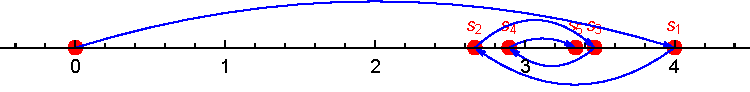
\includegraphics[width=0.8\textwidth]{Figures/altseriestest.pdf}
    \caption{Convergence to sum in the Alternating Series Test.}
    \label{f:altseriestest}
\end{figure}

\begin{example}\label{e:altseriesdiv}
    Determine if the series $\displaystyle \sum_{n = 0}^{\infty} \frac{(-1)^{n}(2n+3)}{5n + 3}$ converges absolutely, converges conditionally, or diverges.

    \begin{solution}
        Note that $\displaystyle \lim_{n \to \infty} \frac{2n+3}{5n+3} = \frac{2}{5} \neq 0$ so by the Alternating Series Test the series diverges.
    \end{solution}
\end{example}

\begin{example}\label{e:altseriesrational}
    Determine if the series $\displaystyle \sum_{n = 0}^{\infty} \frac{(-1)^{n}}{n^{2} + 1}$ converges absolutely, converges conditionally, or diverges.
    \begin{solution}
        Note that $\displaystyle \left| \frac{(-1)^{n}}{n^{2} + 1} \right| = \frac{1}{n^{2} + 1}$ and $\displaystyle 0 < \frac{1}{n^{2} + 1} \leq \frac{1}{n^{2}}$. We know that $\displaystyle \sum_{n=1}^{\infty} \frac{1}{n^{2}}$ is a convergent $p$-series, so by direct comparison $\displaystyle \sum_{n=1}^{\infty} \frac{1}{n^{2} + 1}$ converges so the given series is absolutely convergent.
    \end{solution}
\end{example}

\begin{example}\label{e:altharmonicseries}
    Determine whether the series $\displaystyle \sum_{n=1}^{\infty} \frac{(-1)^{n-1}}{n}$ converges absolutely, converges conditionally, or diverges.
    \begin{solution}
        First we note that $\displaystyle \left| \frac{(-1)^{n-1}}{n} \right| = \frac{1}{n}$ and we know that $\displaystyle \sum_{n=1}^{\infty}\frac{1}{n}$ is a divergent $p$-series, so the given series is not absolutely convergent. However, we do have that $\displaystyle \lim_{n \to \infty} \frac{1}{n} = 0$ and $\displaystyle \frac{1}{n+1} < \frac{1}{n}$ for all $n \geq 1$ so by the Alternating Series Test the given series is convergent. Since it is convergent but not absolutely convergent, it is conditionally convergent.
    \end{solution}
\end{example}

\begin{example}\label{e:Liebnizpiseries}
    Determine whether the series $\displaystyle \sum_{n=1}^{\infty} \frac{4(-1)^{n-1}}{2n -1} = 4 - \frac{4}{3} + \frac{4}{5} - \frac{4}{7} + \cdots$ converges absolutely, converges conditionally, or diverges.
    \begin{solution}
        This is similar to the previous problem; note that $\displaystyle \lim_{n \to \infty} \frac{1}{2n-1} = 0$ and $\displaystyle \frac{1}{2(n+1) - 1} = \frac{1}{2n+1} < \frac{1}{2n-1}$ for all $n \geq 1$. So by the Alternating Series Test, the series is convergent. However, note that by comparison (limit works fine) with $\frac{1}{n}$, a divergent $p$-series, the series is not absolutely convergent so it is conditionally convergent.
    \end{solution}    
    \begin{commentary}
        The reason this one is notable is that, as we will see, the sum is equal to $\pi$! It converges to $\pi$ very slowly, though, as we will see soon.
    \end{commentary}
\end{example}

\subsection{Estimating Sums}

\begin{itemize}
    \item If the series $\sum (-1)^{n-1}a_{n}$ converges by the Alternating Series Test, then $|R_{n}| \leq a_{n+1}$.
    \begin{itemize}
        \item Basic idea:
        \begin{align*}
            R_{n}   &= (-1)^{n}a_{n+1} + (-1)^{n+1}a_{n+2} + (-1)^{n+2}a_{n+3} + (-1)^{n+3}a_{n+4} + \cdots \\
                    &= (-1)^{n}\left( a_{n+1} - a_{n+2} + a_{n+3} - a_{n+4} + \cdots \right)\\
                    &= (-1)^{n}\left( a_{n+1} - \left( a_{n+2} - a_{n+3} + a_{n+4} - \cdots \right) \right) \leq (-1)^{n} a_{n+1}
        \end{align*}
        \item Basically uses the same idea in proof of Alternating Series Test; partial sums will always ping-pong over the sum and the distance to the sum keeps decreasing
    \end{itemize}
\end{itemize}

\begin{example}\label{e:altseriesestsum}
    Find the error in using $s_{10}$ to approximate $\displaystyle \sum_{n=1}^{\infty} \frac{4(-1)^{n-1}}{2n -1}$.
    \begin{solution}
        Here $a_{11} = \frac{4}{21} \approx 0.190476$ so even 10 terms may not get the sum correct to 1 decimal place! 
    \end{solution}

    \begin{commentary}
        We will see later that the sum of this series is exactly $\pi$. Here $s_{10} = 3.04184$ so indeed, it is not even close. To make sure this gets the correct sum to just two decimal places, we would need $\displaystyle a_{n+1} = \frac{4}{2n+1} < 0.005 \Rightarrow n \geq 400$. That's too many for such in imprecise answer. This series converges slowly.
    \end{commentary}    
\end{example}

\subsection{Rearranging Terms of Conditionally Convergent Series}
\begin{itemize}
    \item The alternating harmonic series is
    \[\sum_{n=1}^{\infty} \frac{(-1)^{n-1}}{n}= 1 - \frac{1}{2} + \frac{1}{3} - \frac{1}{4} + \frac{1}{5} - \frac{1}{6} + \cdots = \ln 2.\]
    \item If we multiply each term by $\frac{1}{2}$ we get
    \[\frac{1}{2}\sum_{n=1}^{\infty} \frac{(-1)^{n-1}}{n} = \frac{1}{2} - 	\frac{1}{4} +	 \frac{1}{6} -	 \frac{1}{8} + \frac{1}{10} - \frac{1}{12} + \cdots= \frac{1}{2}\ln 2\]
    \item But if we pad the sum with zeroes (which doesn't change the sum) we get
    \[0 + \frac{1}{2} + 0 -\frac{1}{4} + 0 + \frac{1}{6} + 0 - \frac{1}{8} + 0 + \frac{1}{10} + 0 - \frac{1}{12} + \cdots = \frac{1}{2}\ln 2.\]
    \item Now we add this with the original alternating harmonic series to get:
	\begin{equation*}
		\begin{alignedat}{13}
			&0 + &&\frac{1}{2} + &&0 -				&&\frac{1}{4} + &&0 + 			&&\frac{1}{6} + &&0 - 			&&\frac{1}{8}  + \cdots &&= \frac{1}{2}\ln 2 \\
			+&1 - &&\frac{1}{2} + &&\frac{1}{3} - 	&&\frac{1}{4} + &&\frac{1}{5} - &&\frac{1}{6} + &&\frac{1}{7} - &&\frac{1}{8} + \cdots  &&= \ln 2 \\
			=&1 + &&0 + 		&&\frac{1}{3} -&&\frac{1}{2} + &&\frac{1}{5} + 		&&0 + && \frac{1}{7} - &&\frac{1}{4} + 	\cdots &&= \frac{3}{2}\ln 2
		\end{alignedat}
    \end{equation*}
    \item Now remove the zero terms and note that the resulting series has the same terms of the alternating harmonic series, just in a different order, and gets a different sum!
    \[
        1 + \frac{1}{3} -\frac{1}{2} + \frac{1}{5} + \frac{1}{7} - \frac{1}{4} + \cdots = \frac{3}{2}\ln 2
    \]
    \item Riemann proved that it is possible to make a conditionally convergent series equal to any real number with a suitable rearrangement of terms.
\end{itemize}        

\section{The Ratio and Root Tests}
\setcounter{figure}{0}
\subsection{The Ratio Test}
\begin{enumerate}
    \item If $\displaystyle \lim_{n \to \infty} \left| \frac{a_{n+1}}{a_{n}} \right| < 1$ then $\displaystyle \sum a_{n}$ is absolutely convergent.
    \item If $\displaystyle \lim_{n \to \infty} \left| \frac{a_{n+1}}{a_{n}} \right| > 1$ or equals \(\infty\)then $\displaystyle \sum a_{n}$ is divergent.
    \item If $\displaystyle \lim_{n \to \infty} \left| \frac{a_{n+1}}{a_{n}} \right| = 1$ then the test is inconclusive. \faFrown
\end{enumerate}
\begin{itemize}
    \item This test is great for series with factorial and/or exponential parts in the terms \faSmile
    \item[{\faExclamationTriangle[solid]}] Never use this for rational/algebraic terms! It will always be inconclusive! \faThumbsDown
    \item Generally if all of the terms are positive we need not take the absolute value of the ratio in the test \faSmile
    \item Technically can be used on geometric series \faMeh \ but why do that?
\end{itemize}

\begin{example}\label{e:ratiotestgeolike}
    Determine if the series $\displaystyle \sum_{n=1}^{\infty} \frac{n\cdot 4^{n}}{5^{n}}$ converges absolutely, converges conditionally, or diverges.
    \begin{solution}
        All positive terms \faSmile \ so we take
        \[\lim_{n \to \infty} \frac{(n+1)4^{n+1}}{5^{n+1}} \cdot \frac{5^{n}}{n\cdot 4^{n}} = \lim_{n \to \infty} \frac{4}{5} \cdot \frac{n+1}{n} = \frac{4}{5} < 1\]
        so the series is absolutely convergent.
    \end{solution}
\end{example}

\begin{example}\label{e:ratiotestfact}
    Determine if the series $\displaystyle \sum_{n=1}^{\infty} \frac{n!}{n^{n}}$ converges absolutely, converges conditionally, or diverges.
    \begin{solution}
        Again, all terms are positive \faSmile \ so we take
        \[\lim_{n \to \infty} \frac{(n+1)!}{(n+1)^{n+1}} \cdot \frac{n^{n}}{n!} = \lim_{n \to \infty} \frac{n^{n}}{(n+1)^{n}} = \lim_{n \to \infty} \left( \frac{n+1}{n} \right)^{-n} = \left( \lim_{n \to \infty} \left( 1 + \frac{1}{n} \right)^{n} \right)^{-1} = e^{-1} < 1\]
        so the series is absolutely convergent.
    \end{solution}
\end{example}

\subsection{The Root Test}
\begin{enumerate}
    \item If $\displaystyle \lim_{n \to \infty} \sqrt[n]{|a_{n}|} < 1$ then $\displaystyle \sum a_{n}$ is absolutely convergent.
    \item If $\displaystyle \lim_{n \to \infty} \sqrt[n]{|a_{n}|} > 1$ or equals \(\infty\) then $\displaystyle \sum a_{n}$ is divergent.
    \item If $\displaystyle \lim_{n \to \infty} \sqrt[n]{|a_{n}|} = 1$ then the test is inconclusive. \faFrown
\end{enumerate}
\begin{itemize}
    \item This is basically a specialized case of the Ratio Test that can save some time if terms are to $n$\textsuperscript{th} (or similar, like $n^{2}$) power
\end{itemize}

\begin{example}\label{e:roottestrational}
    Determine if the series $\displaystyle \sum_{n=1}^{\infty} \left( \frac{2n+1}{3n-1} \right)^{n}$ converges absolutely, converges conditionally, or diverges.
    \begin{solution}
        \[\lim_{n \to \infty} \sqrt[n]{\left| \left( \frac{2n+1}{3n-1} \right)^{n} \right|} = \lim_{n \to \infty} \frac{2n+1}{3n-1} = \frac{2}{3} < 1\]
        so the given series is absolutely convergent.
    \end{solution}
\end{example}

\begin{example}\label{e:roottestindetpower}
    Determine if the series $\displaystyle \sum_{n=1}^{\infty} \frac{(-3)^{n}}{n^{4}}$ converges absolutely, converges conditionally, or diverges.
    \begin{solution}
        \[\lim_{n \to \infty} \sqrt[n]{\left| \frac{(-3)^{n}}{n^{4}} \right|} = \lim_{n \to \infty} \frac{3}{(n^{1/n})^{4}} = 3 > 1\]
        (See below for work on $\displaystyle \lim_{n \to \infty} n^{1/n} = 1$. We will use this as a general "known" limit from now on) The series diverges.
    \end{solution}
    \begin{commentary}
        The Root Test works out somewhat nicer here. While on one hand we need to know the special limit, it does save us the trouble of expanding out $(n+1)^{4}$ using the Ratio Test.

        As for $\displaystyle \lim_{n \to \infty} n^{1/n}$, this has the indeterminate form $\infty^{0}$ but we may use L'Hospital's Rule as follows. Let $L = \lim_{n \to \infty} n^{1/n}$. Then
        \begin{align*}
            L       &= \lim_{n \to \infty} n^{1/n} \\
            \ln L   &= \ln \lim_{n \to \infty} n^{1/n}\\
                    &= \lim_{n \to \infty} \ln n^{1/n} \text { (by continuity)}\\
                    &= \lim_{n \to \infty} \tfrac{1}{n}\ln n = \lim_{n \to \infty} \frac{\ln n}{n}\\
            \intertext{ Now this limit has the $\frac{\infty}{\infty}$ for so we use L'Hospital's Rule:}
            \ln L   &= \lim_{n \to \infty} \frac{1}{n} = 0\\
        \end{align*}
        and if $\ln L = 0 \Rightarrow L = e^{0} = 1$.
    \end{commentary}    
\end{example}

\section{Summary of Convergence Tests and Test Strategy}
\setcounter{figure}{0}
\begin{itemize}
    \item Need to pick an appropriate but easy test
    \item What to look for in the terms:
    \begin{itemize}
        \item Geometric? Use that test
        \item Alternating? Use that but look for absolute convergence if asked
        \item Factorial/exponential? Ratio Test
        \item Algebraic with all positive terms? Comparison, usually Limit Comparison
        \item Has an $n$\textsuperscript{th} power? Root Test
        \item Last resort if conditions met and integrable: Integral Test
    \end{itemize}
\end{itemize}

\begin{example}\label{e:seriestestsgeolike}
    Determine if the series $\displaystyle \sum_{n=0}^{\infty} \frac{2^{n}}{3^{n} + 5^{n}}$ converges absolutely, converges conditionally, or diverges.
    \begin{solution}
        This is not a geometric series but we can compare it with one. But this time we might want to use direct comparison. Note that for all $n \geq 1$, $\displaystyle 0 < \left( \frac{2}{3} \right)^{n} = \frac{2^{n}}{3^{n}} < \frac{2^{n}}{3^{n} + 5^{n}}$. So by direct comparison the series is convergent. Further, all of the terms are positive so the series is absolutely convergent.
    \end{solution}
\end{example}

\begin{example}\label{e:seriestestsroot}
    Determine if the series $\displaystyle \sum_{n=0}^{\infty} \frac{n^{3}}{e^{n^{4}}}$ converges absolutely, converges conditionally, or diverges.
    \begin{solution}
        You could use the Integral Test here but justifying it gets messy. \faFrown \ The Ratio Test is better, but still a little messy. \faMeh \ The Root Test is the least messy. \faSmile \ So we take
        \[\lim_{n \to \infty} \sqrt[n]{\left| \frac{n^{3}}{e^{n^{4}}} \right|} = \lim_{n \to \infty} \frac{n^{3/n}}{e^{n^{3}}} = \lim_{n \to \infty} \frac{\left(n^{1/n}\right)^{3}}{e^{n^{3}}} = 0\]
        We use the special limit from Example \ref{e:roottestindetpower}; the numerator approaches 1 as $n \to \infty$. Note that the denominator goes to $\infty$ as $n \to \infty$. Thus the series is absolutely convergent.
    \end{solution}    
\end{example}

\begin{example}\label{e:series-tests-fact}
    Determine if the series $\displaystyle \sum_{n=0}^{\infty} \frac{3^{n}(n!)^{2}}{(2n)!}$ converges absolutely, converges conditionally, or diverges.
    \begin{solution}
        With the factorials present we should try the Ratio Test. Note that
        \[(n!)^{2} = n^{2} \cdot (n-1)^{2} \cdot (n-2)^{2} \cdot \cdots \cdot 2^{2} \cdot 1^{2}\]
        Taking the limit in the Ratio Test and cancelling we get
        \[\lim_{n \to \infty} \frac{3^{n+1}((n+1)!)^{2}}{(2n+2)!} \cdot \frac{(2n)!}{3^{n}(n!)^{2}} = \lim_{n \to \infty} \frac{3(n+1)^{2}}{(2n+2)(2n+1)} = \frac{3}{4} < 1\]
        so the series is absolutely convergent.
    \end{solution}
\end{example}

\begin{example}\label{e:series-tests-factorial-diff}
    Determine if the series $\displaystyle \sum_{k=1}^{\infty} \frac{1}{(k+1)! - k!}$ converges absolutely, converges conditionally, or diverges.
    \begin{solution}
        We need to do some work on the terms first. Note that $(k+1)! - k! = (k+1)k! - k! = k!(k+1-1) = k \cdot k!$. Now we can more easily apply the Ratio Test:
        \[\lim_{n \to \infty} \frac{1}{(k+1)(k+1)!} \cdot \frac{k \cdot k!}{1} = \lim_{n \to \infty} \frac{k}{(k+1)^{2}} = 0 < 1\]
        so the series is absolutely convergent by the Ratio Test.
    \end{solution}
\end{example}

\begin{example}\label{e:seriestestssqrt}
    Determine if the series $\displaystyle \sum_{n=1}^{\infty} \frac{(-1)^{n-1}n}{\sqrt{n^{4} + 1}}$ converges absolutely, converges conditionally, or diverges.

\begin{solution}
    Check for absolute convergence first: looking at the dominant parts of $a_{n} = \frac{n}{\sqrt{n^{4} + 1}}$ we get $b_{n} = \frac{n}{\sqrt{n^{4}}} = \frac{1}{n}$; we know $\sum \frac{1}{n}$ is a divergent $p$-series. Limit comparison will show that the series is not absolutely convergent.

    Now to check for convergence through the Alternating Series Test. First we take the limit of the non-alternating part:
    \[\lim_{n \to \infty} \frac{n}{\sqrt{n^{4} + 1}} = \lim_{n \to \infty} \frac{1}{n} = 0 \text{\; \faThumbsUp}\]
    Now we need to check if the non-alternating part is non-increasing. It will be relatively easier to use derivatives. Let $\displaystyle f(x) = \frac{x}{\sqrt{x^{4} + 1}}$; then
    \[f'(x) = \frac{(x^{4} + 1)^{1/2} - \frac{1}{2}x\cdot(x^{4} + 1)^{-1/2}(4x^{3})}{x^{4} + 1} = \frac{1-3x^{4}}{(x^{4} + 1)^{3/2}}\]
    so we have $f'(x) < 0$ when $x \geq 1$ so the magnitude of the terms is non-increasing. So by the Alternating Series Test, the series is convergent. It is not absolutely convergent, so the series is conditionally convergent.
\end{solution}
\end{example}

\begin{example}\label{e:seriestestsinvtan}
    Determine if the series $\displaystyle \sum_{n=0}^{\infty} \left( \tan^{-1}(n+2) - \tan^{-1} n \right)$ converges absolutely, converges conditionally, or diverges.
    \begin{solution}
        Note that all of the terms are positive. But with each term of the series being a difference we should check for a telescoping sum. The $n$\textsuperscript{th} partial sum is        
        \begin{align*}            
                s_{n}   {}={}   &\sum_{k = 0}^{n-1} \left( \tan^{-1}(k+2) - \tan^{-1} k \right)\\
                        {}={}   &\left( \tan^{-1} 2 - \tan^{-1} 0 \right) + \left( \tan^{-1} 3 - \tan^{-1} 1 \right) + \left( \tan^{-1} 4 - \tan^{-1} 2\right) + \cdots\\
                                & + \left( \tan^{-1}  n  - \tan^{-1} \left( n - 2 \right) \right) + \left( \tan^{-1} \left( n + 1 \right) - \tan^{-1} \left( n - 1 \right) \right)\\
                        {}={}   &\tan^{-1} \left( n + 1 \right) + \tan^{-1}  n - \tan^{-1} 1 = \tan^{-1} \left( n + 1 \right) + \tan^{-1}  n - \frac{\pi}{4}
        \end{align*}
        and now we can take the limit of the partial sum, noting that $\displaystyle \lim_{x \to \infty} \tan^{-1} x = \frac{\pi}{2}$:
        \[S = \lim_{n \to \infty} s_{n} = \lim_{n \to \infty} \left(  \tan^{-1} \left( n + 1 \right) + \tan^{-1}  n - \frac{\pi}{4} \right) = \frac{\pi}{2} + \frac{\pi}{2} - \frac{\pi}{4} = \frac{3\pi}{4}\]
        So the series is absolutely convergent and as a bonus we found its sum \faSmile
     \end{solution}
\end{example}

\begin{example}\label{e:seriestestslog}
    Determine if the series $\displaystyle \sum_{n=3}^{\infty} \frac{(-1)^{n}\ln n}{n}$ converges absolutely, converges conditionally, or diverges.
    \begin{solution}
        First we check for absolute convergence; note that $n \geq 3 > e \Rightarrow \ln n \geq \ln 3 > \ln e = 1$, so $0 < \frac{1}{n} < \frac{\ln n}{n}$ for $n \geq 3$. By direct comparison with the divergent $p$-series $\sum \frac{1}{n}$ the series is not absolutely convergent. (Limit comparison works fine too.) To see if the given series is conditionally convergent we use the Alternating Series Test.

        First we see that $\displaystyle \lim_{n \to \infty} \frac{\ln n}{n} = \lim_{x \to \infty}\frac{\frac{1}{x}}{1} = 0$ by L'Hospital's Rule. Now let $f(x) = \frac{\ln x}{x}$. Taking the derivative we get
        \[f'(x) = \frac{x\cdot \frac{1}{x} - \ln x}{x^{2}} = \frac{1 - \ln x}{x^{2}}   \]
        Remember, $e = 2.71828\ldots < 3$ so with $x \geq 3$ we have $1 - \ln x < 0$ , so $f'(x) < 0$ for all $x \geq 3$. So the magnitude of the terms is non-increasing. The series is convergent by the Alternating Series Test but not absolutely convergent so it is conditionally convergent.
    \end{solution}
\end{example}

\section{Power Series}
\setcounter{figure}{0}
\subsection{Definition, Interval and Radius of Convergence}
\begin{itemize}
    \item A \textbf{power series} is a series of the form
    \[\sum_{n = 0}^{\infty} c_{n} \left( x  - a \right)^{n} = c_{0} + c_{1}(x - a) + c_{2}(x - a)^{2} + \cdots    \]
    \item $a$ is the \textbf{center} of the series; the values $c_{n}$ are the \textbf{coefficients}.
    \item For any power series, exactly one of the following is true:
    \begin{enumerate}
        \item The series converges when $x = a$ \faMeh \; ($R = 0$)
        \item The series converges for all $x$ ($R = \infty$)
        \item The series converges when $|x-a| < R$ for some $R > 0$. $R$ is \textbf{radius of convergence}.
    \end{enumerate}
    \item The Ratio and Root tests are usually the best ones to use; may be able to use Geometric Series test which is easiest \faSmile
    \item[{\faExclamationCircle[solid]}] If $0 < R < \infty$, then the Ratio/Root tests will not determine convergence at the endpoints of the interval; must plug in for $x$ individually and test convergence
\end{itemize}

\begin{example}\label{e:powseriesexp}
    Find the interval and radius of convergence for the power series $\displaystyle \sum_{n=0}^{\infty} \frac{x^{n}}{n!}$.
    \begin{solution}
        Set up the Ratio Test:
        \[\lim_{n \to \infty} \left| \frac{x^{n+1}}{(n+1)!} \cdot \frac{n!}{x^{n}} \right| = \lim_{n \to \infty} \frac{|x|}{n+1} = 0 < 1 \text{ for all } x \in \mathbb{R}\]
        Note that $x$ is constant in this limit. So the series converges for all $x \in \mathbb{R}$, and the radius is $R = \infty$.
    \end{solution}
\end{example}

\begin{example}\label{e:powserieszerorad}
    Find the interval and radius of convergence for the power series $\displaystyle \sum_{n=0}^{\infty} n! x^{n}$.
    \begin{solution}
        Ratio Test again:
        \[\lim_{n \to \infty} \left| \frac{(n+1)!x^{n+1}}{n! x^{n}} \right| = \lim_{n \to \infty} (n+1)|x|\]
        This limit will only exist when $x=0$; for any other $x$ the limit is $\infty$. So the radius is $R=0$.
    \end{solution}
\end{example}

\begin{example}\label{e:powseriesinterval}
    Find the interval and radius of convergence for the power series $\displaystyle \sum_{n=1}^{\infty} \frac{(3x+2)^{n}}{n}$.
    \begin{solution}
        Ratio Test!
        \[\lim_{n \to \infty} \left| \frac{(3x+2)^{n+1}}{n+1} \cdot \frac{n}{(3x+2)^{n}} \right| = \lim_{n \to \infty} \frac{n}{n+1} |3x + 2| = |3x + 2|\]
        For the series to converge by the Ratio Test, we need $|3x + 2| < 1 \Rightarrow -1 < x < -\frac{1}{3}$; so $R = \frac{1}{3}$. But we need to check the endpoints here.

        When $x=-1$ the series becomes $\displaystyle \sum_{n=1}^{\infty} \frac{(-1)^{n}}{n}$; this is the Alternating Harmonic Series and we already found it was convergent in Example \ref{e:altharmonicseries}. When $x = -\frac{1}{3}$, the series becomes $\displaystyle \sum_{n=1}^{\infty} \frac{1}{n}$, the Harmonic Series, a divergent $p$-series. Thus the interval of convergence is \(-1 \leq x < \frac{1}{3}\).
    \end{solution}
\end{example}

\section{Power Series Representations of Functions}
\setcounter{figure}{0}
\subsection{Geometric-like Power Series}
\begin{itemize}
    \item Very basic power series:
    \[\sum_{n=0}^{\infty} x^{n} = 1 + x + x^{2} + x^{3} + x^{4} + \cdots   \]
    \item This is a geometric series with ratio $x$
    \item Converges when $|x| < 1$ and sum is $\frac{1}{1-x}$
    \item But this is a function, so we can let this power series represent this function.
    \item Note that the power series is only defined when $|x| < 1$ but the function $f(x) = \frac{1}{1-x}$ is only undefined when $x \neq 1$
    \item We can make function in the form $\frac{a}{1-r}$ into a power/geometric series
\end{itemize}

\begin{example}\label{e:powseriesgeolike}
    Write the function $\displaystyle f(x) = \frac{3}{2+x}$ as a power series, then find the interval and radius of convergence.
    \begin{solution}
        We need to get this function in the right form first:
        \[f(x) = \frac{3}{2+x} = \frac{\frac{3}{2}}{1 - \left( -\frac{x}{2} \right)}\]
        now it is the sum of a convergent geometric series with $a = \frac{3}{2}$, $r = -\frac{x}{2}$. So we can write        
        \[f(x) = \sum_{n = 0}^{\infty} \frac{3}{2}\left( -\frac{x}{2} \right)^{n} = 3\sum_{n=0}^{\infty} \frac{(-1)^{n} x^{n}}{2^{n+1}}\]
        This series converges when $\left| -\frac{x}{2} \right| < 1 \Rightarrow -2 < x < 2$, so $R=2$. Because the series is geometric it diverges at the endpoints of the interval.
    \end{solution}
\end{example}

\begin{example}\label{e:powseriesparfrac}
    Write the function $\displaystyle f(x) = \frac{4x+4}{x^{2} - 4}$ as a power series, then find the interval and radius of convergence.
    \begin{solution}
        This does not look like the form we need but we can do partial fraction decomposition then get them in the proper form of a geometric series sum: 
        \[\frac{4x+4}{x^{2} - 4} = \frac{1}{x+2} + \frac{3}{x-2} = \frac{\frac{1}{2}}{1-\left( -\frac{x}{2} \right)} - \frac{\frac{3}{2}}{1-\frac{x}{2}}\]
        Now we can get power series for each individually:
        \[\frac{\frac{1}{2}}{1-\left( -\frac{x}{2} \right)} - \frac{\frac{3}{2}}{1-\frac{x}{2}} = \sum_{n=0}^{\infty} \frac{(-1)^{n}x^{n}}{2^{n+1}} - \sum_{n=0}^{\infty} \frac{3x^{n}}{2^{n+1}} = \sum_{n=0}^{\infty} \frac{(-3 + (-1)^{n})x^{n}}{2^{n+1}}\]
        Note that the two geometric series converged when $-2 < x < 2$, so their sum does as well.
    \end{solution}
\end{example}

\begin{example}\label{e:reciprocal-series}
    Find a power series for \(f(x) = \dfrac{1}{x}\) centered at 2.
    \begin{solution}
        First we need the function to look like the sum of a convergent geometric series:
        \[\frac{1}{x} = \frac{1}{1 + (x - 1)} = \frac{1}{1-(-(x-1))}\]
        Now it looks like a geometric series sum with \(a=1, r = (-(x-1))\). So in series form we have, when \(|-(x-1)|< 1 \Rightarrow 0 < x < 2\), 
        \[\sum_{n=0}^{\infty} (-(x-1))^n = \sum_{n=0}^{\infty} (-1)^n (x-1)^n = \frac{1}{x}\]
    \end{solution}
\end{example}

So if we have a power series that's convergent over at least an interval of values, we can treat it like a function! We plug in something for \(x\), we get a real number! \faThumbsUp

\subsection{Differentiation and Integrals}
\begin{itemize}
    \item Let $\displaystyle f(x) = \sum_{n = 0}^{\infty} c_{n} \left( x  - a \right)^{n}$
    \item Can take derivative by just taking the Power Rule on each term
    \begin{itemize}
        \item $\displaystyle f'(x) = \sum_{n = 0}^{\infty} n c_{n} \left( x  - a \right)^{n-1}$
        \item Note that depending on $c_{n}$ we may have a 0 term at the beginning; can discard
    \end{itemize}
    \item Can take antiderivative with Power Rule too
    \begin{itemize}
        \item $\displaystyle \int \! f(x) \, dx = C + \sum_{n = 0}^{\infty} \frac{c_{n} \left( x  - a \right)^{n+1}}{n+1}$
    \end{itemize}
    \item Derivative and antiderivative will have the same center and radius of convergence
    \item[{\faExclamationCircle[solid]}] Behavior at endpoints may change!
    \item We can use this to find series for derivatives or integrals of functions for which series are easier to find \faThumbsUp 
\end{itemize}

\begin{example}\label{e:powseriesinvtan}
    Find a power series for $f(x) = \tan^{-1} x$ centered at 0 then find its interval and radius of convergence.
    \begin{solution}
        The function itself isn't very series-friendly but $\displaystyle f'(x) = \frac{1}{1 + x^{2}}$ is! \faSmile
        \[f'(x) = \frac{1}{1 + x^{2}} = \frac{1}{1 - (-x^{2})} = \sum_{n = 0}^{\infty} (-x^{2})^{n} = \sum_{n = 0}^{\infty} (-1)^{n}x^{2n}\]
        The series converges when $|-x^{2}| < 1 \Rightarrow -1 < x < 1$. Now we take the antiderivative to get
        \[f(x) = C + \sum_{n = 0}^{\infty} \frac{(-1)^{n} x^{2n+1}}{2n+1}\]
        To get $C$ we use the fact that $f(0) = \tan^{-1} 0 = 0$; plugging $x=0$ into the series gives us $f(0) = C + 0 = 0 \Rightarrow C = 0$. So we have
        \[\tan^{-1} x = \sum_{n = 0}^{\infty} \frac{(-1)^{n} x^{2n+1}}{2n+1}\]
        We still need to check the endpoints $x = \pm 1$. When $x=-1$ the series becomes $\displaystyle \sum_{n = 0}^{\infty} \frac{(-1)^{n} (-1)^{2n+1}}{2n+1} = \sum_{n = 0}^{\infty} \frac{(-1)^{n+1}}{2n+1}$ which is convergent by the Alternating Series Test. (Note that $(-1)^{2n+1} = -1$ as $2n+1$ is always odd.) Likewise when $x=1$ the series becomes $\displaystyle \sum_{n = 0}^{\infty} \frac{(-1)^{n}}{2n+1}$ which is just the negative of the series we just tested so it is convergent too.

        Thus the interval of convergence is $[-1, 1]$ and $R=1$.
    \end{solution}
    \begin{commentary}
        Note that since this series converges at $x=1$ we have
        \[4\tan^{-1} 1 = \sum_{n = 0}^{\infty} \frac{4(-1)^{n}}{2n+1} = 4 - \frac{4}{3} + \frac{4}{5} - \frac{4}{7} + \cdots = 4\cdot \frac{\pi}{4} = \pi\]
        We saw this series back in Example \ref{e:Liebnizpiseries}. This series is the \textbf{Leibniz Series for Pi}. This series converges very slowly, though. By the error estimate in the Alternating Series Test, in order to correctly approximate $\pi$ to two decimal places we need $\displaystyle a_{n+1} = \frac{4}{2n+3} < 0.005 \Rightarrow n \geq 400$. \faFrown \ That is way too many terms for such an imprecise result!

        There are series for approximating $\pi$ much more quickly. This one is due to Ramanujan:
        \[\frac{1}{\pi} = \frac{2\sqrt{2}}{99^{2}}\sum_{n=0}^{\infty} \frac{(4n)!}{n!^{4}}\frac{26390n+1103}{396^{4n}}\]
        While messy \faMeh \ this converges much more quickly. In fact the first term (then the reciprocal) gets within 6 decimal digits of $\pi$; just three terms approximate $\pi$ correctly to 15 digits!
    \end{commentary}
\end{example}

\begin{example}\label{e:powseriesintegrate}
    Find a power series for $\displaystyle f(x) = -\frac{1}{(x+3)^{2}}$ centered at 0 then find its interval and radius of convergence.
    \begin{solution}
        We note that this is the derivative of $\displaystyle F(x) = \frac{1}{x+3}$ so we start by finding a series for $F$:
        \[F(x) = \frac{1}{x+3} = \frac{\frac{1}{3}}{1-(-\frac{x}{3})} = \frac{1}{3} \sum_{n=0}^{\infty} \left( -\frac{x}{3} \right)^{n} = \sum_{n=0}^{\infty} \frac{(-1^{n})x^{n}}{3^{n+1}}\]
        Taking the derivative of the series we get the series for $f$:
        \[f(x) = \frac{d}{dx}\sum_{n=0}^{\infty} \frac{(-1^{n})x^{n}}{3^{n+1}} = \sum_{n=1}^{\infty} \frac{(-1^{n})n x^{n-1}}{3^{n+1}}\]
        If we plug in $x = \pm 3$, we get series where the terms do not approach 0, so the series is divergent at both values. Thus the interval of convergence is $(-3, 3)$.
    \end{solution}
\end{example}

\begin{example}\label{e:powseriesintandderiv}
    Find the derivative and antiderivative of the power series $\displaystyle \sum_{n=0}^{\infty} \frac{x^{n}}{n!} = 1 + x + \frac{x^2}{2!} + \frac{x^{3}}{3!} + \cdots$.
    \begin{solution}
        First, the derivative:
        \[\frac{d}{dx} \sum_{n=0}^{\infty} \frac{x^{n}}{n!} = \sum_{n=1}^{\infty} \frac{x^{n-1}}{(n-1)!} = \sum_{n=0}^{\infty} \frac{x^{n}}{n!}\]
        \ldots so this power series is its own derivative! Where have we seen \textit{that} before?

        Next, the antiderivative:
        \[\int \sum_{n=0}^{\infty} \frac{x^{n}}{n!} \, dx = C + \sum_{n=0}^{\infty} \frac{x^{n+1}}{(n+1)!} = C + \sum_{n=1}^{\infty} \frac{x^{n}}{n!} = C + x + \frac{x^2}{2!} + \frac{x^{3}}{3!} + \cdots\]
        so the antiderivative is the same except for possibly a constant term. \textit{Very} familiar! \faSmile
    \end{solution}
\end{example}

\begin{example}
    Find a power series for \(f(x) = \ln x\) centered at 1.
    \begin{solution}
        This function does not lend itself well to a power series at first, but we can work with the derivative:
        \[f'(x) = \frac{1}{x} = \frac{1}{1+x-1} = \frac{1}{1-(1-x)} = \frac{1}{1-[-1(x-1)]}\]
        which is now in the sum of a geometric series form! So now at least when \(|x-1|<1 \Rightarrow 0 < x < 2\) we have
        \[f'(x) = \frac{1}{1-[-1(x-1)]} = \sum_{n=0}^{\infty} (-1)^{n}(x-1)^{n}\]
        Now integrating we get
        \[f(x) = C + \sum_{n=0}^{\infty} \frac{(-1)^{n}(x-1)^{n+1}}{n+1}\]
        and with \(\ln 1 = 0, C = 0\); also, when \(x = 0\) the above series diverges and converges when \(x=2\).
    \end{solution}
\end{example}

\section{Taylor and Maclaurin Series}
\setcounter{figure}{0}
\subsection{General Form of Analytic Functions}
\begin{itemize}
    \item Suppose $f$ is a function with a power series representation (called an \textbf{analytic function}), i.e. $f(x) = c_{0} + c_{1} (x - a) + c_{2} (x-a)^{2} + c_{3} (x-a)^{3} + \cdots $
    \item We we start taking derivatives we get:
    \begin{alignat*}{6}
        f'(x)   &=   {}&c_{1}{} +   &2c_{2} (x-a)  &{}   &+  &{}  3&c_{3} (x-a)^{2}    &+ \cdots\\
        f''(x)  &=   {}&{}{}        &2c_{2}        &{}   &+  &{}  2 \cdot 3&c_{3}(x-a) &+ \cdots\\
        f'''(x) &=   {}&{}{}        &{}            &{}   &{} &{}  2 \cdot 3&c_{3}      &+ \cdots\\
        \vdots
    \end{alignat*}
    \item Plugging in $a$ for $x$ in each we get:
    \begin{align*}
        f(a)    &= c_{0} \\
        f'(a)   &= c_{1} \\
        f''(a) &= 2 c_{2} \\
        f'''(a) &= 3! c_{3}\\
        \vdots \\
        f^{(n)}(a) &= n! c_{n}\\
        \vdots
    \end{align*}
    \item So in general $c_{n} = \dfrac{f^{(n)}(a)}{n!}$. So the general form of an analytic function is
    \[\sum_{n=0}^{\infty} \frac{f^{(n)}(a)}{n!} (x-a)^{n}\]
    \item We call this the \textbf{Taylor Series of $\bm{f}$ centered at $\bm{a}$}.
    \item When $a=0$, we call this the \textbf{Maclaurin series of $\bm{f}$}.
\end{itemize}

% TODO #6 Change tables to tabu

\begin{example}\label{e:Taylorseriesexp}
    Find a Maclaurin series for $f(x) = e^{x}$.
    \begin{solution}
        We need to find a pattern to the derivatives. A table of them is shown in Table \ref{t:MaclaurinExp}.
        \begin{table}[htbp]\label{t:MaclaurinExp}
            \centering
            \caption{First few coefficients for Maclaurin series for $f(x) = e^{x}$.}
            \begin{tabular}{cccc}
                $\bm{n}$    & $\bm{f^{(n)}}$    & $\bm{f^{(n)}(0)}$ & $\bm{\frac{f^{(n)}(0)}{n!} x^{n}}$ \\ \hline
                0           & $e^{x}$           & 1                 & 1 \\[6pt]
                1           & $e^{x}$           & 1                 & $x$ \\[6pt]
                2           & $e^{x}$           & 1                 & $\frac{x^{2}}{2}$ \\[6pt]
                3           & $e^{x}$           & 1                 & $\frac{x^{3}}{3!}$ \\[6pt]
                4           & $e^{x}$           & 1                 & $\frac{x^{4}}{4!}$ \\[6pt]
                5           & $e^{x}$           & 1                 & $\frac{x^{5}}{5!}$ \\[6pt]
                6           & $e^{x}$           & 1                 & $\frac{x^{6}}{6!}$ \\[6pt]
                $n$         & $e^{x}$           & 1                 & $\frac{x^{n}}{n!}$ \\[6pt]
                \hline
            \end{tabular}
        \end{table}
    So the Maclaurin series is the series $\displaystyle \sum_{n=0}^{\infty} \frac{x^{n}}{n!}$ from Example \ref{e:powseriesexp}!
    \end{solution}
    \begin{commentary}
        We still have not shown that $\displaystyle e^{x} = \sum_{n=0}^{\infty} \frac{x^{n}}{n!}$ \ldots yet. Also this is not the usual way for us to find these as it can be difficult to find a pattern to the terms.

        It is worth noting that in Differential Equations we have a theorem that says given an equation of the form $y' = f(x,y)$ with initial value $f(x_{0}) = y_{0}$, if $f$ and $f_{y}$ are continuous in an area around the point $(x_{0}, y_{0})$, then the equation has a unique solution. In other words, if both $y'_{1} = f(x,y)$, $y_{1}(x_{0}) = y_{0}$ and $y'_{2} = f(x,y)$, $y_{2}(x_{0}) = y_{0}$ then $y_{1} = y_{2}$.

        So if we let $y_{1} = e^{x}$ and $\displaystyle y_{2} = \sum_{n=0}^{\infty} \frac{x^{n}}{n!}$, both satisfy the equation $y' = y$ and the initial condition $y(0)=1$. So they are in fact the same and $\displaystyle e^{x} = \sum_{n=0}^{\infty} \frac{x^{n}}{n!}$. Note also that the series converges for all real $x$.
    \end{commentary}
\end{example}

\subsection{Taylor's Inequality}
\begin{itemize}
    \item Usually do not have nice differential equations to help us \faMeh
    \item Let $\displaystyle R_{n} = f(x) - \sum_{k=0}^{n-1} \frac{f^{(k)}(a)}{k!} (x-a)^k$
    \item Want to show that $R_{n} \to 0$ as $n \to \infty$
    \item The more general way to show that a function is equal to its Taylor series is with \textbf{Taylor's Inequality}:
    \[\text{If } \left| f^{(n+1)}(x) \right| \leq M \text{ when } |x - a| \leq d \text{ then } |R_{n}| \leq \frac{M}{(n+1)!}|x - a|^{n+1} \text{ when } |x - a| \leq d\]
    \item This gives us a bound on the remainder
    \item For any Taylor series we have
    \[|R_{n}| = \frac{|f^{(n+1)}(z)|}{(n+1)!}|x-a|^{n+1}    \]
    for some $z$ between $x$ and $a$.
    \item We're not going to worry about this too much.
\end{itemize}

\subsection{Other Functions}
\begin{itemize}
    \item The \textbf{Binomial Series}: Let $f(x) = (1+x)^{k}, k \in \mathbb{R}, |x| < 1$. Then we have
    \[(1 + x)^{k} = \sum_{n = 0}^{\infty} \binom{k}{n} x^{n} \]
    \item $\displaystyle \binom{k}{n} = \frac{k(k-1)(k-2)\cdots (k-(n-1))}{n!}$, $n \in \mathbb{N}$, $k \in \mathbb{R}$ is the \textbf{binomial coefficient}. By definition, \(\binom{k}{0} \binom{k}{k}= 1\).
\end{itemize}

\begin{example}\label{e:binomial-coefficients}
    Calculate each binomial coefficient.
    \begin{enumerate}[label=\textbf{\alph*.}]
        \item $\displaystyle \binom{6}{2} = \frac{6\cdot 5}{2!} = 15$
        \item $\displaystyle \binom{\frac{2}{3}}{3} = \frac{\frac{2}{3} \cdot \left( -\frac{1}{3} \right) \cdot \left( -\frac{4}{3} \right)}{3!} = \frac{4}{81}$
    \end{enumerate}
\end{example}

\begin{example}\label{e:binomseries}
    Find the first four terms of a Maclaurin series for $\displaystyle f(x) = \frac{1}{\sqrt{x + 1}} = (1 + x)^{-1/2}$.
    \begin{solution}
        \begin{align*}
            (1 + x)^{-1/2}  &= \sum_{n = 0}^{\infty} \binom{-\frac{1}{2}}{n} x^{n}\\
                            &= 1 - \frac{1}{2} x + \frac{\Big( -\frac{1}{2} \Big)\Big( -\frac{3}{2} \Big)}{2} x^{2} + \frac{\Big( -\frac{1}{2} \Big)\Big( -\frac{3}{2} \Big)\Big( -\frac{5}{2} \Big)}{3!} x^{3} + \cdots\\
                            &= 1 - \frac{1}{2} x^{2} + \frac{3}{8} x^{2} - \frac{5}{16} x^{3} + \cdots
        \end{align*}
    \end{solution}
\end{example}

\begin{itemize}
    \item Some other good series to know:
    \begin{itemize}
        \item $\displaystyle \sin x = \sum_{n = 0}^{\infty} \frac{(-1)^{n}x^{2n+1}}{(2n+1)!}$
        \item $\displaystyle \cos x = \sum_{n = 0}^{\infty} \frac{(-1)^{n}x^{2n}}{(2n)!}$
    \end{itemize}
    \item If $f$ has a power series, we can get a power series for $f(cx^{p})$ by just plugging in $cx^{p}$ into the series for $f(x)$ \faSmile
    \item Can also distribute a term like $cx^{p}$ through a series to get a series for $cx^{p} f(x)$
    \item We can also integrate and differentiate as well
\end{itemize}

\begin{example}\label{e:Macseriescos}
    Find a Maclaurin series for $f(x) = \cos x^{3}$.
    \begin{solution}
        Plug in $x^{3}$:
        \[\cos x^{3} = \sum_{n = 0}^{\infty} \frac{(-1)^{n}(x^{3})^{2n}}{(2n)!} = \sum_{n = 0}^{\infty} \frac{(-1)^{n}x^{6n}}{(2n)!}\]
    \end{solution}
\end{example}

\begin{example}\label{e:Macseriesexp}
    Find a Maclaurin series for $f(x) = x^{5} e^{x}$.
    \begin{solution}
        Just distribute:
        \[x^{5} e^{x} = x^{5} \sum_{n=0}^{\infty} \frac{x^{n}}{n!} = \sum_{n=0}^{\infty} \frac{x^{n+5}}{n!}\]
    \end{solution}
\end{example}

\begin{example}\label{e:Macserieserf}
    Calculate $\displaystyle \int_{0}^{1} e^{-x^{2}} \, dx$ with a maximum error of 0.0005.
    \begin{solution}
        This function does not have an elementary antiderivative. \faFrown \ But we can use a series to get a not-so-elementary one! \faSmile \ Start by getting the Maclaurin series for the function:
        \[e^{-x^{2}} = \sum_{n=0}^{\infty} \frac{(-x^{2})^{n}}{n!} = \sum_{n=0}^{\infty} \frac{(-1)^{n} x^{2n}}{n!}\]
        Integrating both sides with respect to $x$ we get:
        \[\int e^{-x^{2}} \, dx = C + \sum_{n=0}^{\infty} \frac{(-1)^{n} x^{2n+1}}{(2n+1)n!}\]
        Now apply the Fundamental Theorem of Calculus:
        \[\int_{0}^{1} e^{-x^{2}} \, dx = \sum_{n=0}^{\infty} \frac{(-1)^{n}}{(2n+1)n!}\]
        To get $R_{n} < 0.0005$ and we use the error bound for the Alternating Series Test:
        \[a_{n+1} = \frac{1}{(2n+3)(n+1)!} < 0.0005 \Leftrightarrow n \geq 5\]
        So calculating $s_{5}$ will give us a partial sum within 0.0005 of the actual value of the integral:
        \[\sum_{n=0}^{5} \frac{(-1)^{n}}{(2n+1)n!} = 1 - \frac{1}{3} + \frac{1}{10} - \frac{1}{42} + \frac{1}{216} = \frac{31049}{41580} \approx 0.746729\]
        Mathematica gives a result of $0.74682$ for the integral so this is not too bad. The error from $s_{6}$ is about $0.0000949361$ so this is pretty good.
    \end{solution}
\end{example}

\subsection{Evaluating Limits with Taylor Series}

Some limits can be evaluated by replacing some functions in the limit with its Taylor Series and simplifying. This is how many computer algebra systems evaluate them.

\begin{example}
    Use Taylor series to evaluate \(\displaystyle \lim_{x \to 0} \frac{x^3 - 3x + 3\tan^{-1}x }{x^5}\).
    \begin{solution}
        \begin{align*}
            \lim_{x \to 0} \frac{x^3 - 3x + 3\tan^{-1}x }{x^5} &= \lim_{x \to 0} \frac{x^3 - 3x - 3\left(\sum_{n=0}^{\infty} (-1)^n \frac{x^{2n+1}}{2n+1}\right)}{x^5}\\
            &= \lim_{x \to 0} \frac{x^3 - 3x + \left(3x - x^3 + \frac{3x^5}{5} - \frac{3x^7}{7} + \cdots\right)}{x^5}\\
            &= \lim_{x \to 0} \left(\frac{3}{5} + \frac{3x^2}{7} - \frac{3x^5}{7} + \cdots\right)\\
            &= \frac{3}{5}
        \end{align*}
    \end{solution}
\end{example}

\subsection{Proof of the Basel Problem (Optional)}
This proof of the Basel Problem is taken from \url{https://en.wikipedia.org/wiki/Basel_problem}.
\begin{theorem}
	$\displaystyle \sum_{n=1}^{\infty}\frac{1}{n^2} = \frac{\pi^2}{6}$.
\end{theorem}

\begin{proof}
    We know that this $p$-series is convergent as $p=2>1$. To find the sum of the series, we will start with the Maclaurin series of the sine function:

    \[\sin x = \sum_{n=0}^{\infty} \frac{(-1)^n x^{2n+1}}{(2n+1)!} = x - \frac{x^3}{3!} + \frac{x^5}{5!} - \frac{x^7}{7!} + \cdots\]
    Dividing each term by $x$ we get 
    \[\frac{\sin x}{x} = 1 - \frac{x^2}{3!} + \frac{x^4}{5!} - \frac{x^6}{7!} + \cdots\]

    Note that the roots of $\frac{\sin x}{x}$ are all integer multiples of $\pi$. We know that finite polynomials can all be factored down into linear products of its roots (e.g. $f(x) = x^2 - 6x + 8 = (x-2)(x-4)$). The Weierstrass Factorization Theorem states that we can do the same for infinite polynomials too. Here's the problem with the proof as presented by Euler at the time: this theorem would not be proven for another century! Euler \textit{assumed} this was true. Fortunately for his proof, it is.

    We need a constant term of 1, so instead of factoring the series as $(x-\pi)(x+\pi)(x-2\pi)(x+2\pi)\cdots$ which means we need to divide by a constant to get a constant term of 1, we will factor as
    \[\frac{\sin x}{x} = \left(1-\frac{x}{\pi}\right)\left(1+\frac{x}{\pi}\right) \left(1-\frac{x}{2\pi}\right) \left(1+\frac{x}{2\pi}\right)\left(1-\frac{x}{3\pi}\right) \left(1+\frac{x}{3\pi}\right)\left(1-\frac{x}{4\pi}\right) \left(1+\frac{x}{4\pi}\right)\cdots\]
    We can then multiply pairs of factors using $(a-b)(a+b) = a^2-b^2$ to get
    \[
                        \frac{\sin x}{x} = \left(1-\frac{x^2}{\pi^2}\right)\left(1-\frac{x^2}{4\pi^2}\right)\left(1-\frac{x^2}{9\pi^2}\right)\left(1-\frac{x^2}{16\pi^2}\right)\cdots\]
    So now we will multiply this out paying attention to the coefficients on the $x^2$ term. We get the coefficient on the $x^2$ term as
    \[-\left(\frac{1}{\pi^2} + \frac{1}{4\pi^2} + \frac{1}{9\pi^2} + \frac{1}{16\pi^2}\cdots\right)= -\frac{1}{\pi^2}\sum_{n=1}^{\infty}\frac{1}{n^2}.\]
    But the coefficient for $x^2$ in the original series for $\frac{\sin x}{x}$ is $-\frac{1}{3!} = -\frac{1}{6}$. Thus
    \[-\frac{1}{\pi^2}\sum_{n=1}^{\infty}\frac{1}{n^2} = -\frac{1}{6} .\]
    Now we need only multiply both sides by $-\pi^2$ to get
    \[\sum_{n=1}^{\infty}\frac{1}{n^2} = \frac{\pi^2}{6}.\]
\end{proof}

Now since the Weierstrass Factorization Theorem was not yet proven and so he did not have a rigorous proof, Euler demonstrated that his result of $\frac{\pi^2}{6}$ was correct by calculating partial sums of the series to 20 decimal places and comparing them to $\frac{\pi^2}{6} \approx 1.6449340668482264365$ to 20 places. He did not do this by directly calculating the partial sums, though, as that would take a very long time. How long? The series is convergent by the Integral Test, so an upper bound on using the $n$\textsuperscript{th} partial sum to approximate the series is given by
\[R_n < \int_n^\infty \frac{1}{x^2} dx = \frac{1}{n}.\]
But by this bound in order to guarantee the partial sum is correct to 20 decimal places we would need $2 \times 10^{20}$ terms! (It actually \textit{only} takes over a quintillion terms but still...) Rather than do this, Euler had another tool for estimating partial sums called \textit{Euler-Maclaurin Summation}. This technique was discovered by Euler and Colin Maclaurin independently. The idea is to use an integral and a fast-converging series to estimate the value of a slowly-converging series like the one in the Basel Problem. In general, Euler-Maclaurin summation states that
\[
	\sum_{i=a}^{b} f(i) = \int_{b}^{a} f(x)\, dx + \frac{f(b)+f(a)}{2} + \sum_{k=1}^{\infty} \frac{B_{2k}}{(2k)!}\left(f^{(2k-1)}(b) - f^{(2k-1)}(a)\right)\]
where $B_{2k}$ is the $2k$\textsuperscript{th} Bernoulli number, which can be calculated using
\[B_{2k} = \sum_{i=0}^{2k}\sum_{j=0}^{i} (-1)^{j} \binom{i}{j}\frac{j^{2k}}{i+1}.\]
(Whew!) So Euler used the faster-converging series on the right side to approximate the slowly converging series $\sum \frac{1}{n^2}$.

But due to the factorization of series not being proven at the time this was not then a true proof. This would not be accepted today. It is  possible for a series to be very close to a value but not equal to it. For example, take the expression
\[\left(\frac{1}{10^5} \sum_{n=-\infty}^{\infty} e^{-n^2/10^{10}}\right)^2\]
 The series is convergent by the Ratio Test. This expression's sum matches $\pi = 3.141592654\ldots$ to over 42 billion digits... after which it does not. It is very, \textit{very} close, but not equal, to $\pi$. Note that the value of this series is not surprising given that $\displaystyle \int_{-\infty}^{\infty} e^{-x^{2}} \, dx = \sqrt{\pi}$; the series is just like a Riemann sum for the integral with $\Delta x = 10^{-5}$.

\subsection{The Sum of the Natural Numbers (Optional)}
So some string theorists (lol) on YouTube claimed that
\[S = \sum_{n=1}^{\infty} n = 1 + 2 + 3 + 4 + \cdots  = -\frac{1}{12} \text{\faMeh}\]

They start by defining the series
\begin{alignat*}{2}
    S_{1} &= \sum_{n=1}^{\infty} (-1)^{n-1}     &&= 1 - 1 + 1 + 1 - 1 + \cdots \\
    S_{2} &= \sum_{n=1}^{\infty} (-1)^{n-1} n   &&= 1 - 2 + 3 - 4 + 5 - \cdots
\end{alignat*}
Then they claim that
\[S_{1} = \sum_{n=1}^{\infty} (-1)^{n-1} = 1 - 1 + 1 + 1 - 1 + \cdots = \frac{1}{2}.\]
They reason that $\frac{1}{2}$ is the average of the partial sums so that's \textit{the} sum. They go on by adding $S_{2}$ to itself with a zero term:
\begin{alignat*}{10}
        &S_{2} {\,}&&= {\,}&&1 - {\,}&&2 + {\,}&&3 - {\,}&&4 + {\,}&&5 - {\,}&&6 {\,}+ {\,}&&\cdots&&\\
    +   &S_{2} &&= &&0 {\,}+ &&1 {\,}- &&2 {\,}+ &&3 {\,}- &&4 {\,}+ &&5 {\,}- &&\cdots&&\\
    =  2&S_{2} &&= &&1 {\,}- &&1 {\,}+ &&1 {\,}- &&1 {\,}+ &&1 {\,}- &&1 {\,}+ &&\cdots &&= S_{1} = \frac{1}{2} 
\end{alignat*}
So they claim $S_{2} = \frac{1}{4}$. \faMeh \, But then they set up $S - S_{2}$ to get 
\begin{alignat*}{10}
    &S {\,} &&= {\,}&&1 + {\,}&&2 + {\,}&&3 + {\,}&&4 + {\,}&&5 + {\,}&&6 + &&\cdots&&\\
-   &S_{2}  &&=    -&&1 {\,}+ &&2 {\,}- &&3 {\,}+ &&4 {\,}- &&5 {\,}+ &&6 - &&\cdots&&\\
   &       &&=     &&0 {\,}+ &&4 {\,}+ &&0 {\,}+ &&8 {\,}+ &&0 {\,}+ &&12 {\,}+ &&\cdots &&= 4S 
\end{alignat*}
now with $S - S_{2} = 4S$ and $S_{2} = \frac{1}{4}$, $S = -\frac{1}{12}$. \faFrown \;
This argument is incredibly flawed and is based, at the beginning, by the false premise that $S_{1} = \frac{1}{2}$. 

A big issue here is that we cannot manipulate divergent series the same way with the same rules as we do convergent series. Indeed, using the same manipulations in different ways can produce contradictory results. We can take
\begin{alignat*}{9}
    &S  &&=    {\,}&& 1 + {\,}    && 2 + {\,}    && 3 + {\,}    && 4 + {\,}    && 5 + {\,} &&\cdots \\
   +&S  &&=         && 0 {\,}+     && 1 {\,}+     && 2 {\,}+     && 3 {\,}+     && 4 {\,}+  &&\cdots \\
   =2&S &&=         && 1 {\,}+     && 3 {\,}+     && 5 {\,}+     && 7 {\,}+     && 9 {\,}+  &&\cdots
\end{alignat*}
But we also have $2S = 2 + 4 + 6 + 8 + \cdots$; now we can take $2S + 2S = 1 + 2 + 3 + 4 + 5 + \cdots = 4S = S \Rightarrow 3S = 0 \Rightarrow S = 0$. \faMeh

So while all of the series mentioned in the video are divergent, as it turns out there are actually relationships between these divergent series and these values!

\begin{definition}\label{d:abel-sum}
    The \textbf{Abel Sum} of the sequence $\{a_{n}\}_{n=1}^{\infty}$ is $\displaystyle A = \lim_{x \to 1^{-}} \sum_{n=1}^{\infty} a_{n} x^{n-1}$, if the limit exists.
\end{definition}

Let's look at $S_{1}$ first. We can set up its Abel sum as
\begin{align*}
    A_{1}   &= \lim_{x \to 1^{-}} \sum_{n=0}^{\infty} (-1)^{n} x^{n}\\
            &= \lim_{x \to 1^{-}} \sum_{n=0}^{\infty} (-x)^{n}\\
            \intertext{But this is a geometric series that converges when $|x|<1$! so}
    A_{1}   &= \lim_{x \to 1^{-}} \frac{1}{1+x} = \frac{1}{2}
\end{align*}
and there it is! So the series is divergent, but its \textit{Abel sum} is $\frac{1}{2}$.

Now let's look at $S_{2}$ and its Abel sum, $A_{2}$:
\[A_{2}   = \lim_{x \to 1^{-}} \sum_{n=1}^{\infty} (-1)^{n-1} n x^{n-1}\]
This is not a geometric series, but its antiderivative is! Let $a_{2}(x) = \sum_{n=1}^{\infty} (-1)^{n-1} n x^{n-1}$. Then
\begin{align*}
    \int a_{2} (x) \, dx    &= C + \sum_{n=1}^{\infty} \frac{(-1)^{n-1} nx^{n}}{n} = C - \sum_{n=1}^{\infty} (-x)^{n}\\
                            &= C - \frac{x}{1+x}, |x| < 1
    \intertext{and then taking the derivative we have}
    a_{2} (x)               &= \frac{1}{(1+x)^{2}}, |x| < 1
\end{align*}
and so $\displaystyle A_{2} = \lim_{x \to 1^{-}} \frac{1}{(1+x)^{2}} = \frac{1}{4}$, the same value in the video.

That is as far as Abel sums can take us, though. If we try to do the same for the sum $S$ with an Abel sum we get
\[A =  \lim_{x \to 1^{-}} \sum_{n=1}^{\infty}  n x^{n-1}\].
This is not geometric but we can let $\displaystyle a(x) = \sum_{n=1}^{\infty}  n x^{n-1}$ and integrate to get
\[\int a(x) \, dx = \sum_{n=1}^{\infty}  x^{n} = \frac{x}{1-x}\]
when $|x| < 1$. So then for $|x|<1$ we have $a(x) = \frac{d}{dx}\left( -1 + \frac{1}{1-x} \right)= -\frac{1}{(1-x)^{2}}$. But then we have
\[ A =  \lim_{x \to 1^{-}} -\frac{1}{(1-x)^{2}} \]
which does not exist. The series $S$ is not summable using any method that is \textit{linear} or \textit{stable}.

\begin{definition}\label{d:summation-props}
    Let \((a_{n}) = \{a_{1}, a_{2}, a_{3},\ldots\}\). A summation method \(\mathcal{S}(a_{n})\) is \textbf{regular} if it sums convergent series to their sums under ordinary summation. \(\mathcal{S}(a_{n})\) is \textbf{linear} if for sequences \((a_{n})\) and \((b_{n})\) and a scalar \(c\), \(\mathcal{S}((a_{n}) + c(b_{n})) = \mathcal{S}(a_{n}) + c\mathcal{S}(b_{n})\). \(\mathcal{S}\) is \textbf{stable} if the \textbf{shift rule} apples. That is, for any positive integer \(N\), \(\mathcal{S}(a_{n})\) converges if and only if \(\mathcal{S}(a_{n+N})\) converges.
\end{definition}

And yet there are ways of associating the sum \(S\) with the value \(-\frac{1}{12}\). The \(n\)\textsuperscript{th} partial sum of \(S\) is
\[s_{n} = \sum_{k=1}^{n} k = \frac{n(n+1)}{2}\]
so we can look at the function \(f(x) = \frac{x(x+1)}{2}\) and see what happens!

\newpage\thispagestyle{firstofchapter}
\chapter{Parametric and Polar Equations}
\section{Parametric Equations}
\setcounter{figure}{0}
\subsection{Introducing the Parameter}

\begin{itemize}
    \item So far we usually had $y = f(x)$ but not all curves have this relation, e.g. unit circle
    \item A curve may repeat $x$ or $y$ coordinates
    \item Think of curve like a track someone is walking on
    \item At any moment in \textit{time} they can only be in one place, i.e. $x$ and $y$ coordinates are unique at any given moment
    \item Introduce the \textbf{parameter} $t$ and let $x = x(t)$, $y = y(t)$
    \item Positive orientation in direction of increasing $t$
\end{itemize}

\begin{example}\label{e:parametricparabola}
    Describe the parametric curve with equations $x = \sqrt{t}$, $y=t$.
    \begin{solution}
        Note that $y = x^{2}$ but $x = \sqrt{t} \geq 0, t \in \mathbb{R}$. A plot of the curve where $0 \leq t \leq 2$ is given in Figure \ref{f:parapara}.
    \end{solution}      
\end{example}

\begin{example}\label{e:paraellipse}
    Describe the parametric curve with equations $x = 2\cos t$, $y= 3\sin t$.
    \begin{solution}
        While there isn't a nice way to solve for the parameter to get an equation, we do have an equation relating $\sin t$ and $\cos t$, namely $\sin^{2} \theta + \cos^{2} t  = 1$. Solving for $\sin t$ and $\cos t$ here we get $\displaystyle \cos t = \dfrac{x}{2}, \sin t = \frac{y}{3} \Rightarrow \left( \frac{x}{2} \right)^{2} + \left( \frac{y}{3} \right)^{2} = 1 \Rightarrow \frac{x^{2}}{4} + \frac{y^{2}}{9} = 1$, an ellipse. A plot where $0 \leq t \leq 2\pi$ is given in Figure \ref{f:paraellipse}. 
    \end{solution}
\end{example}
\begin{figure}[htbp]
    \centering
    \begin{minipage}{0.45\textwidth}
        \centering
        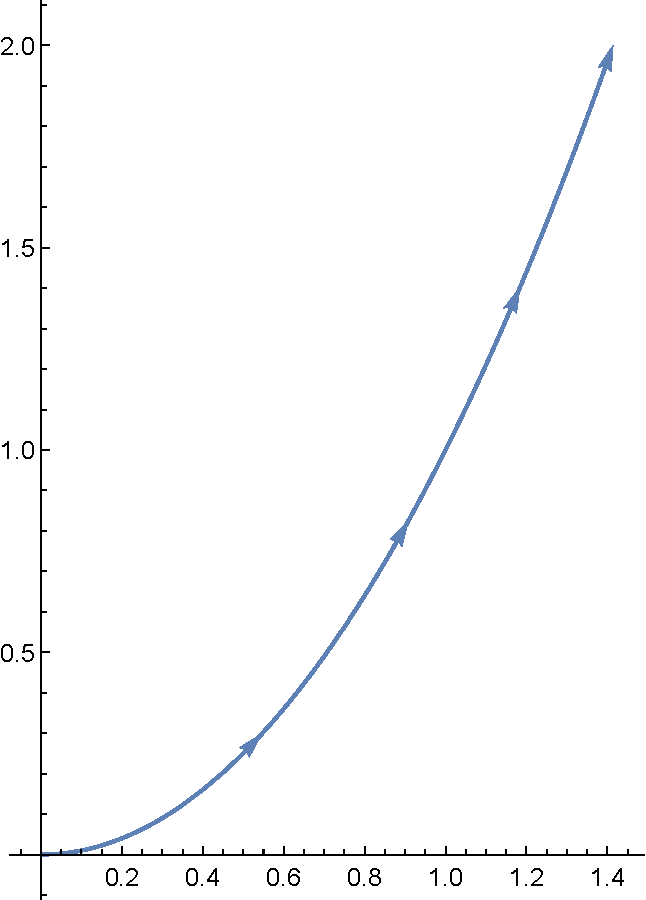
\includegraphics[width=0.6\textwidth]{Figures/parapara.pdf}
        \caption{Plot of curve in Example \ref{e:parametricparabola}.}
        \label{f:parapara}
    \end{minipage}\hfill
    \begin{minipage}{0.45\textwidth}
        \centering
        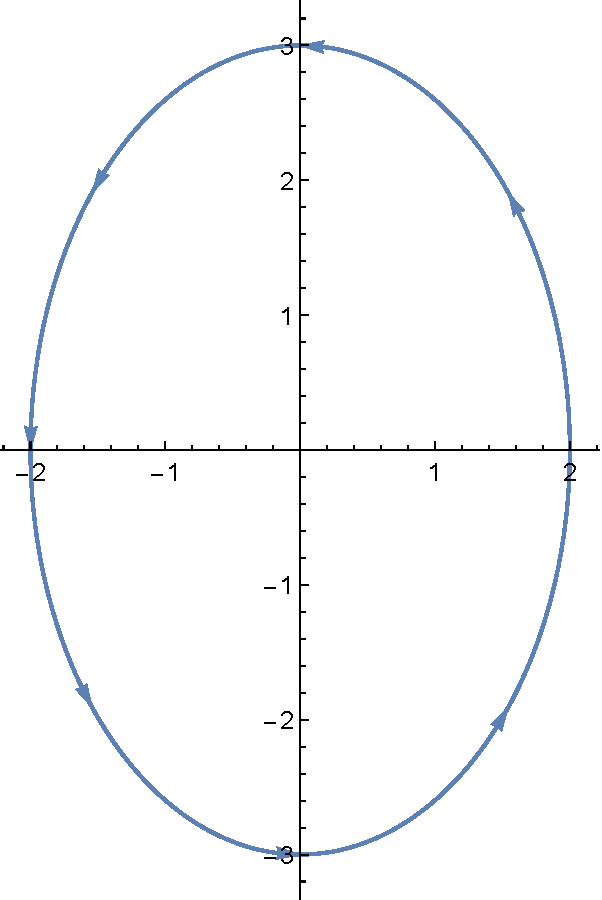
\includegraphics[width=0.6\textwidth]{Figures/paraellipse.pdf}
        \caption{Plot of curve in Example \ref{e:paraellipse}.}
        \label{f:paraellipse}
    \end{minipage}\hfill
\end{figure}

\begin{example}
    Find parametric equations of a circle centered at \((-2, 3)\) with a radius of 4.
    \begin{solution}
        One way to think of this is to take the circle centered at the origin first then translate it to the desired center. A circle with radius 4 centered at the origin would have parametric equations \(x = 4 \cos t, y = 4 \sin t\). Translating these to move the center to \((-2, 3)\) we have \(x = 4\cos t - 2, y = 4\sin t + 3\).
    \end{solution}
\end{example}

\begin{example}
    Find parametric equations of the line segment between the points \((1, -3)\) and \((4,4)\).
    \begin{solution}
        Key is to look at the change in coordinates. \(x\) changes by \(3\) from start to finish and \(y\) changes by 7. If we only let \(0 \leq t \leq 1\), we can set \(x = 1 + 3t\) and \(y = -3 + 7t\).
    \end{solution}
\end{example}

\subsection{Derivatives and Parametric Curves}

\begin{itemize}
    \item Slope of tangent line: $\dfrac{dy}{dx}$; same thing here!
    \item Want the rate of change in $y$ with respect to $x$
    \item $x'(t) = \dfrac{dx}{dt}, y'(t) = \dfrac{dy}{dy} \Rightarrow dx = x'(t) dt, dy = y'(t) dt \Rightarrow \dfrac{dy}{dx} = \dfrac{y'(t)}{x'(t)}$
\end{itemize}

\begin{example}\label{e:paraslope}
    Find the slope of the tangent line to the parametric curve defined by $x = t^{2} + 1, y = \frac{1}{2}(t+1)$ when $t = 3$.
    \begin{solution}
        \[\frac{dy}{dx} = \frac{\frac{1}{2}}{2t} = \frac{1}{4t}\]
        Plugging in $t = 3$ we get $\displaystyle m = \frac{dy}{dx}\bigg|_{t = 3} = \frac{1}{12}$. The curve and the tangent line are shown in Figure \ref{f:paraslope}.
    \end{solution}
\end{example}
\begin{figure}[htbp]
    \centering
        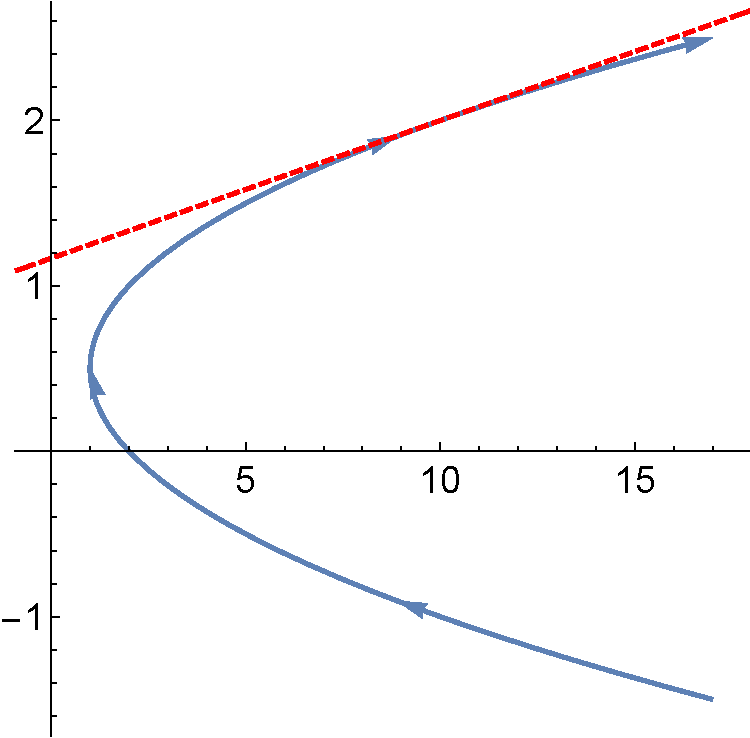
\includegraphics[width=0.25\textwidth]{Figures/paraslope.pdf}
    \caption{Curve and tangent line in Example \ref{e:paraslope}.}
    \label{f:paraslope}
\end{figure}

\begin{itemize}
    \item We can also find $\frac{d^{2}y}{dx^{2}}$ to get the rate of change in the slope of the tangent line or the concavity of the curve. We just take the derivative again, basically replacing $y$ with $\frac{dy}{dx}$:
    \[\frac{d^{2}y}{dx^{2}} = \frac{d}{dx} \frac{dy}{dx} = \frac{\frac{d}{dt} \frac{dy}{dx}}{\frac{dx}{dt}}\]
    \item Take derivative of $\frac{dy}{dx}$ with respect to $t$ again, then divide by $\frac{dx}{dt}$
\end{itemize}

\begin{example}\label{e:paraconcavity}
    Find the concavity of the curve $x = t^{2} + 1, y = \frac{1}{2}(t+1)$ when $t=3$.
    \begin{solution}
        We already found in Example \ref{e:paraslope} that $\frac{dy}{dx} = \frac{\frac{1}{2}}{2t} = \frac{1}{4t}$ so here we have
        \[\frac{d^{2}y}{dx^{2}} = \frac{\frac{d}{dt} \frac{1}{4t}}{2t} = -\frac{1}{8t^3}\]
        When $t=3$ we have $\displaystyle \frac{d^{2}y}{dx^{2}}\bigg|_{t=3} = -\frac{1}{216}$ so the curve is concave down.
    \end{solution}
\end{example}

\subsection{Arc Length of Parametric Curves}

\begin{itemize}
    \item We can go back to our previous work on arc length of $y = f(x)$
    \item We had $\Delta L = \sqrt{(\Delta x)^{2} + (\Delta y)^{2}}$
    \item Now we can put these in terms of $t$:
    \[\sqrt{(\Delta x)^{2} + (\Delta y)^{2}} = \sqrt{\left( \frac{dx}{dt} \right)^{2} + \left( \frac{dy}{dt} \right)^{2}}\, dt\]
    \item So the length along the curve when $a \leq t \leq b$ isn
    \[L = \int_{a}^{b} \sqrt{\left( \frac{dx}{dt} \right)^{2} + \left( \frac{dy}{dt} \right)^{2}}\, dt\]
\end{itemize}

\begin{example}\label{e:paralength}
    Find the length along the parametric curve defined by $x = t^{2} + 1, y = 4t^{3}, 0 \leq t \leq 1$.
    \begin{solution}
        \[\int_{0}^{1} \sqrt{4t^{2} + 144t^{2}} \, dt = \int_{0}^{1} 2t \sqrt{1 + 36t^{2}}\, dt = \frac{1}{54}\left( 37\sqrt{37} - 1 \right)\]
        Using the substitution $u = 1 + 36t^2 \Rightarrow du = 72t \, dt$.
    \end{solution}
\end{example}

\section{Polar Coordinates}
\setcounter{figure}{0}

\begin{itemize}
    \item Cartesian/rectangular coordinates aren't always the best \faMeh
    \item Now we call the origin the \textbf{pole} and the positive $x$-axis the \textbf{polar axis}.
    \item Instead describe point by direction to face to from origin ($\theta$) and \textit{signed} distance to go ($r$)
    \item $r>0$: go forward $r$ units; $r<0$: go backwards $r$ units \faMeh
    \begin{itemize}
        \item Usually best to make $r \geq 0$ and $0 \leq \theta < 2\pi$ or if in Quadrant IV $-\frac{\pi}{2} \leq \theta \leq 0$
    \end{itemize}
    \item See Figure \ref{f:polarpoint} for point $(r, \theta)$
    \item Converting rectangular $\leftrightarrow$ polar coordinates:
    \begin{itemize}
        \item $r^{2} = x^{2} + y^{2}$
        \item $\tan \theta = \frac{y}{x}$ \faExclamationTriangle[solid] \ Watch the quadrant!
        \item $x = r \cos \theta$; $y = r \sin \theta$ 
    \end{itemize}
\end{itemize}
\begin{figure}[htbp]
    \centering
        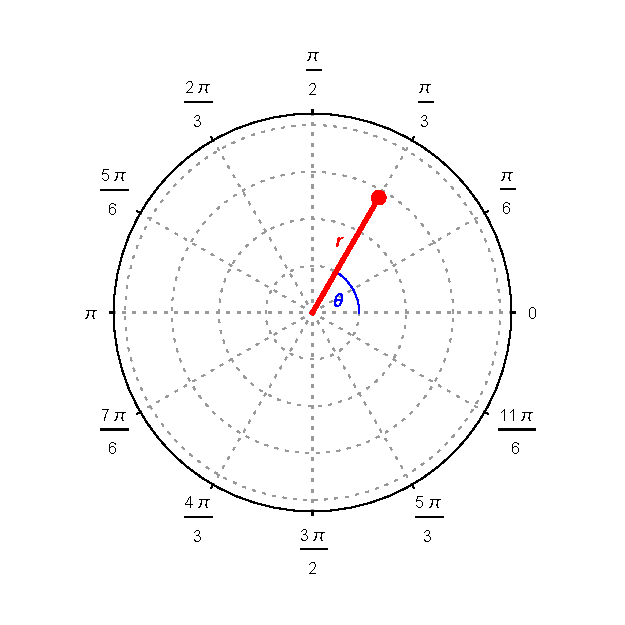
\includegraphics[width = 0.4\textwidth]{Figures/polarpoint.pdf}
    \caption{Polar point $(r, \theta)$.}
    \label{f:polarpoint}
\end{figure}

\begin{example}\label{e:polarconvpoints}
    Convert each of the following points:
    \begin{enumerate}[label=\alph*.]
        \item $(-4\sqrt{3}, -4)$ to polar
        \begin{solution}
            $r^{2} = \left( -4\sqrt{3} \right)^{2} + (-4)^{2} = 64 \Rightarrow r = 8$; $\tan \theta = \frac{1}{\sqrt{3}}$ but this point is in the third quadrant so we use $\theta = \frac{7\pi}{6}$. The polar point is $(8, \frac{7\pi}{6})$. 
        \end{solution}
        \item $\left( -3, \frac{3\pi}{4} \right)$ to rectangular
        \begin{solution}
            $x = -3 \cos \frac{3\pi}{4} = \frac{3}{\sqrt{2}}$; $y = -3 \sin \frac{3\pi}{4} = -\frac{3}{\sqrt{2}}$; the rectangular point is $\left(\frac{3}{\sqrt{2}} , -\frac{3}{\sqrt{2}} \right)$.
        \end{solution}
    \end{enumerate}
\end{example}

\begin{example}\label{e:polarconvs}
    Convert each equation to rectangular form and graph it.
    \begin{enumerate}
        \item $r = 3$\label{e:polarcircle}
        \begin{solution}
            This can be done with the conversion equations but let's think about it; this is all points 3 units away from the origin. It's a circle with radius 3! The rectangular equation is $x^{2} + y^{2} = 9$. A graph is in Figure \ref{f:polarcircle}.
        \end{solution}

        \item $\displaystyle \theta = \frac{\pi}{6}$\label{e:polarthetaline}
        \begin{solution}
            This is the set of points that makes an angle of $\frac{\pi}{6}$ with the polar axis but $r$ can be anything. This is a line through the pole. A graph is in Figure \ref{f:polarthetaline}.
        \end{solution}

        \item $r = \dfrac{12}{3\sin \theta - 6\cos \theta}$
        \begin{solution}
            \[r = \frac{12}{3\sin \theta - 6\cos \theta} \Rightarrow 3r \sin \theta - 6r \cos \theta = 12 \Rightarrow 3y - 6x = 12 \Rightarrow y = 2x + 4\]
            \begin{commentary}
                Note that the original polar function is undefined at the angle $\theta$ that runs parallel to the line. Here $\theta \approx 63.4^{\circ}$.
            \end{commentary}
        \end{solution}
    \end{enumerate}    
\end{example}
\begin{figure}[htbp]
    \centering
    \begin{minipage}{0.45\textwidth}
        \centering
        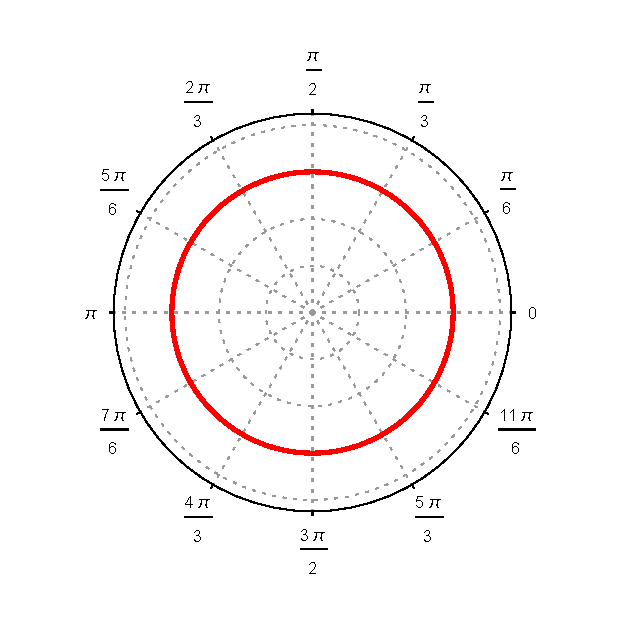
\includegraphics[width=0.6\textwidth]{Figures/polarcircle.pdf}
        \caption{Plot of curve in Example \ref{e:polarconvs}\ref{e:polarcircle}.}
        \label{f:polarcircle}
    \end{minipage}\hfill
    \begin{minipage}{0.45\textwidth}
        \centering
        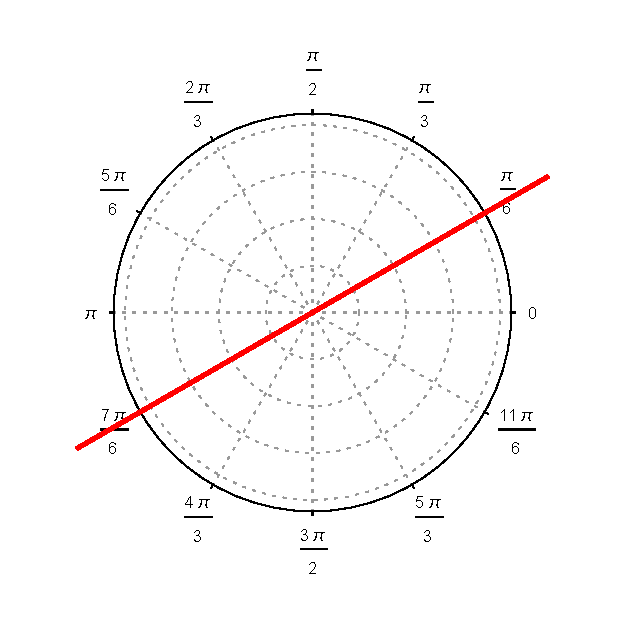
\includegraphics[width=0.6\textwidth]{Figures/polarthetaline.pdf}
        \caption{Plot of curve in Example \ref{e:polarconvs}.}
        \label{f:polarthetaline}
    \end{minipage}\hfill
\end{figure}

\section{Calculus and Polar Coordinates}
\setcounter{figure}{0}
\subsection{Slopes of Tangent Lines}

\begin{itemize}
    \item This is an \textit{excellent} example of when memorization is bad
    \item Start with conversion equations: $x = r \sin \theta$, $y = r \cos \theta$
    \item If we have $r = f(\theta)$ then conversion equations become $x = f(\theta) \sin \theta$, $y = f(\theta) \cos \theta$
    \item Now they are all in terms of $\theta$ so we can treat them as parametric equations and find the slope!
    \[\frac{dy}{dx} = \frac{\frac{dy}{d\theta}}{\frac{dx}{d\theta}} = \frac{f(\theta)\cos \theta + f'(\theta)\sin \theta}{-f(\theta) \sin \theta + f'(\theta)\cos \theta}\]
    \item[{\faExclamationCircle[solid]}] Please do not just try to memorize this \faFrown \ Re-derive it with the polar conversion equations instead \faSmile
\end{itemize}

\begin{example}\label{e:polarslope}
    Find the slope of the tangent line to the polar graph $f(\theta) = 2 - 3\sin \theta$ when $\theta = \pi$.
    \begin{solution}
        This will be much easier if we pre-calculate everything. Here $f(\pi) = 2$; $f'(\theta) = -3 \cos \theta \Rightarrow f'(\pi) = 3$. Now we just plug in!
        \[\frac{dy}{dx} = \frac{(2)(-1) + (3)(0)}{-(2)(0) + (3)(-1)} = \frac{2}{3}\]
        The graph of the function and the tangent line are shown in Figure \ref{f:polarslope}.
    \end{solution}
\end{example}

\begin{figure}[htbp]
    \centering
        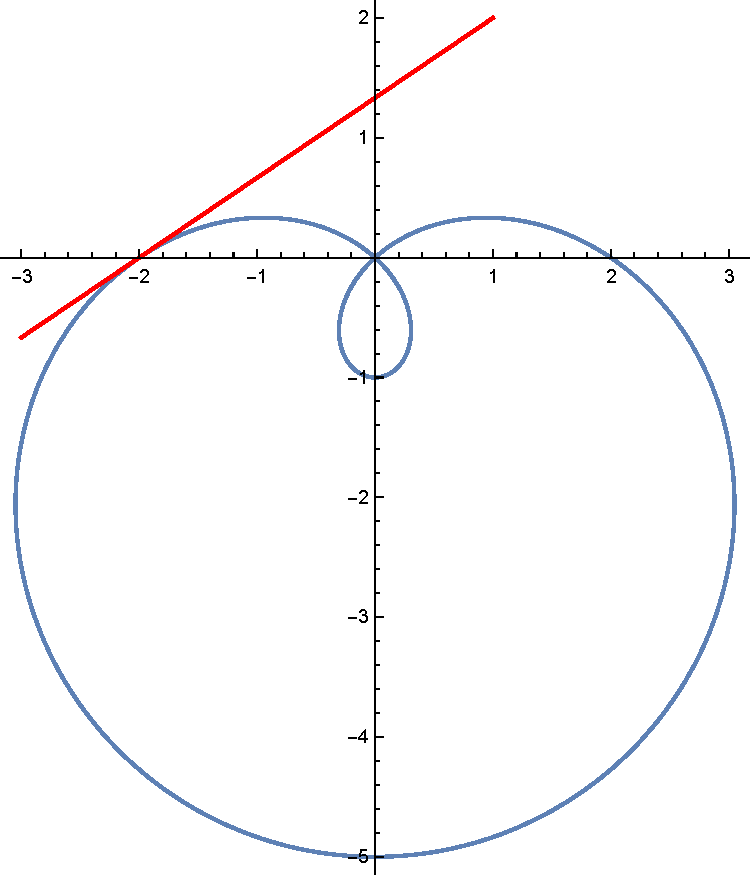
\includegraphics[width = 0.3\textwidth]{Figures/polarslope.pdf}
    \caption{Curve and tangent line in Example \ref{e:polarslope}.}
    \label{f:polarslope}
\end{figure}

\subsection{Areas of Polar Regions}
\begin{itemize}
    \item Instead of rectangles, use circular sectors to approximate area
    \item $A = \frac{1}{2}r^{2} \theta$
    \item With $r = f(\theta)$ and going over an angle of $\Delta \theta$ we have $A = \frac{1}{2} [f(\theta)]^{2} \Delta \theta$
    \item Do the usual add these all up, take limit as $\Delta \theta \to 0$, we have the definite integral \faSmile
    \[A = \frac{1}{2} \int_{a}^{b} [f(\theta)]^{2} \, d\theta\]
    \item Set up shown in Figure \ref{f:polarrects}.
    \item Half-angle identities will be helpful here
\end{itemize}

\begin{figure}[htbp]
    \centering
        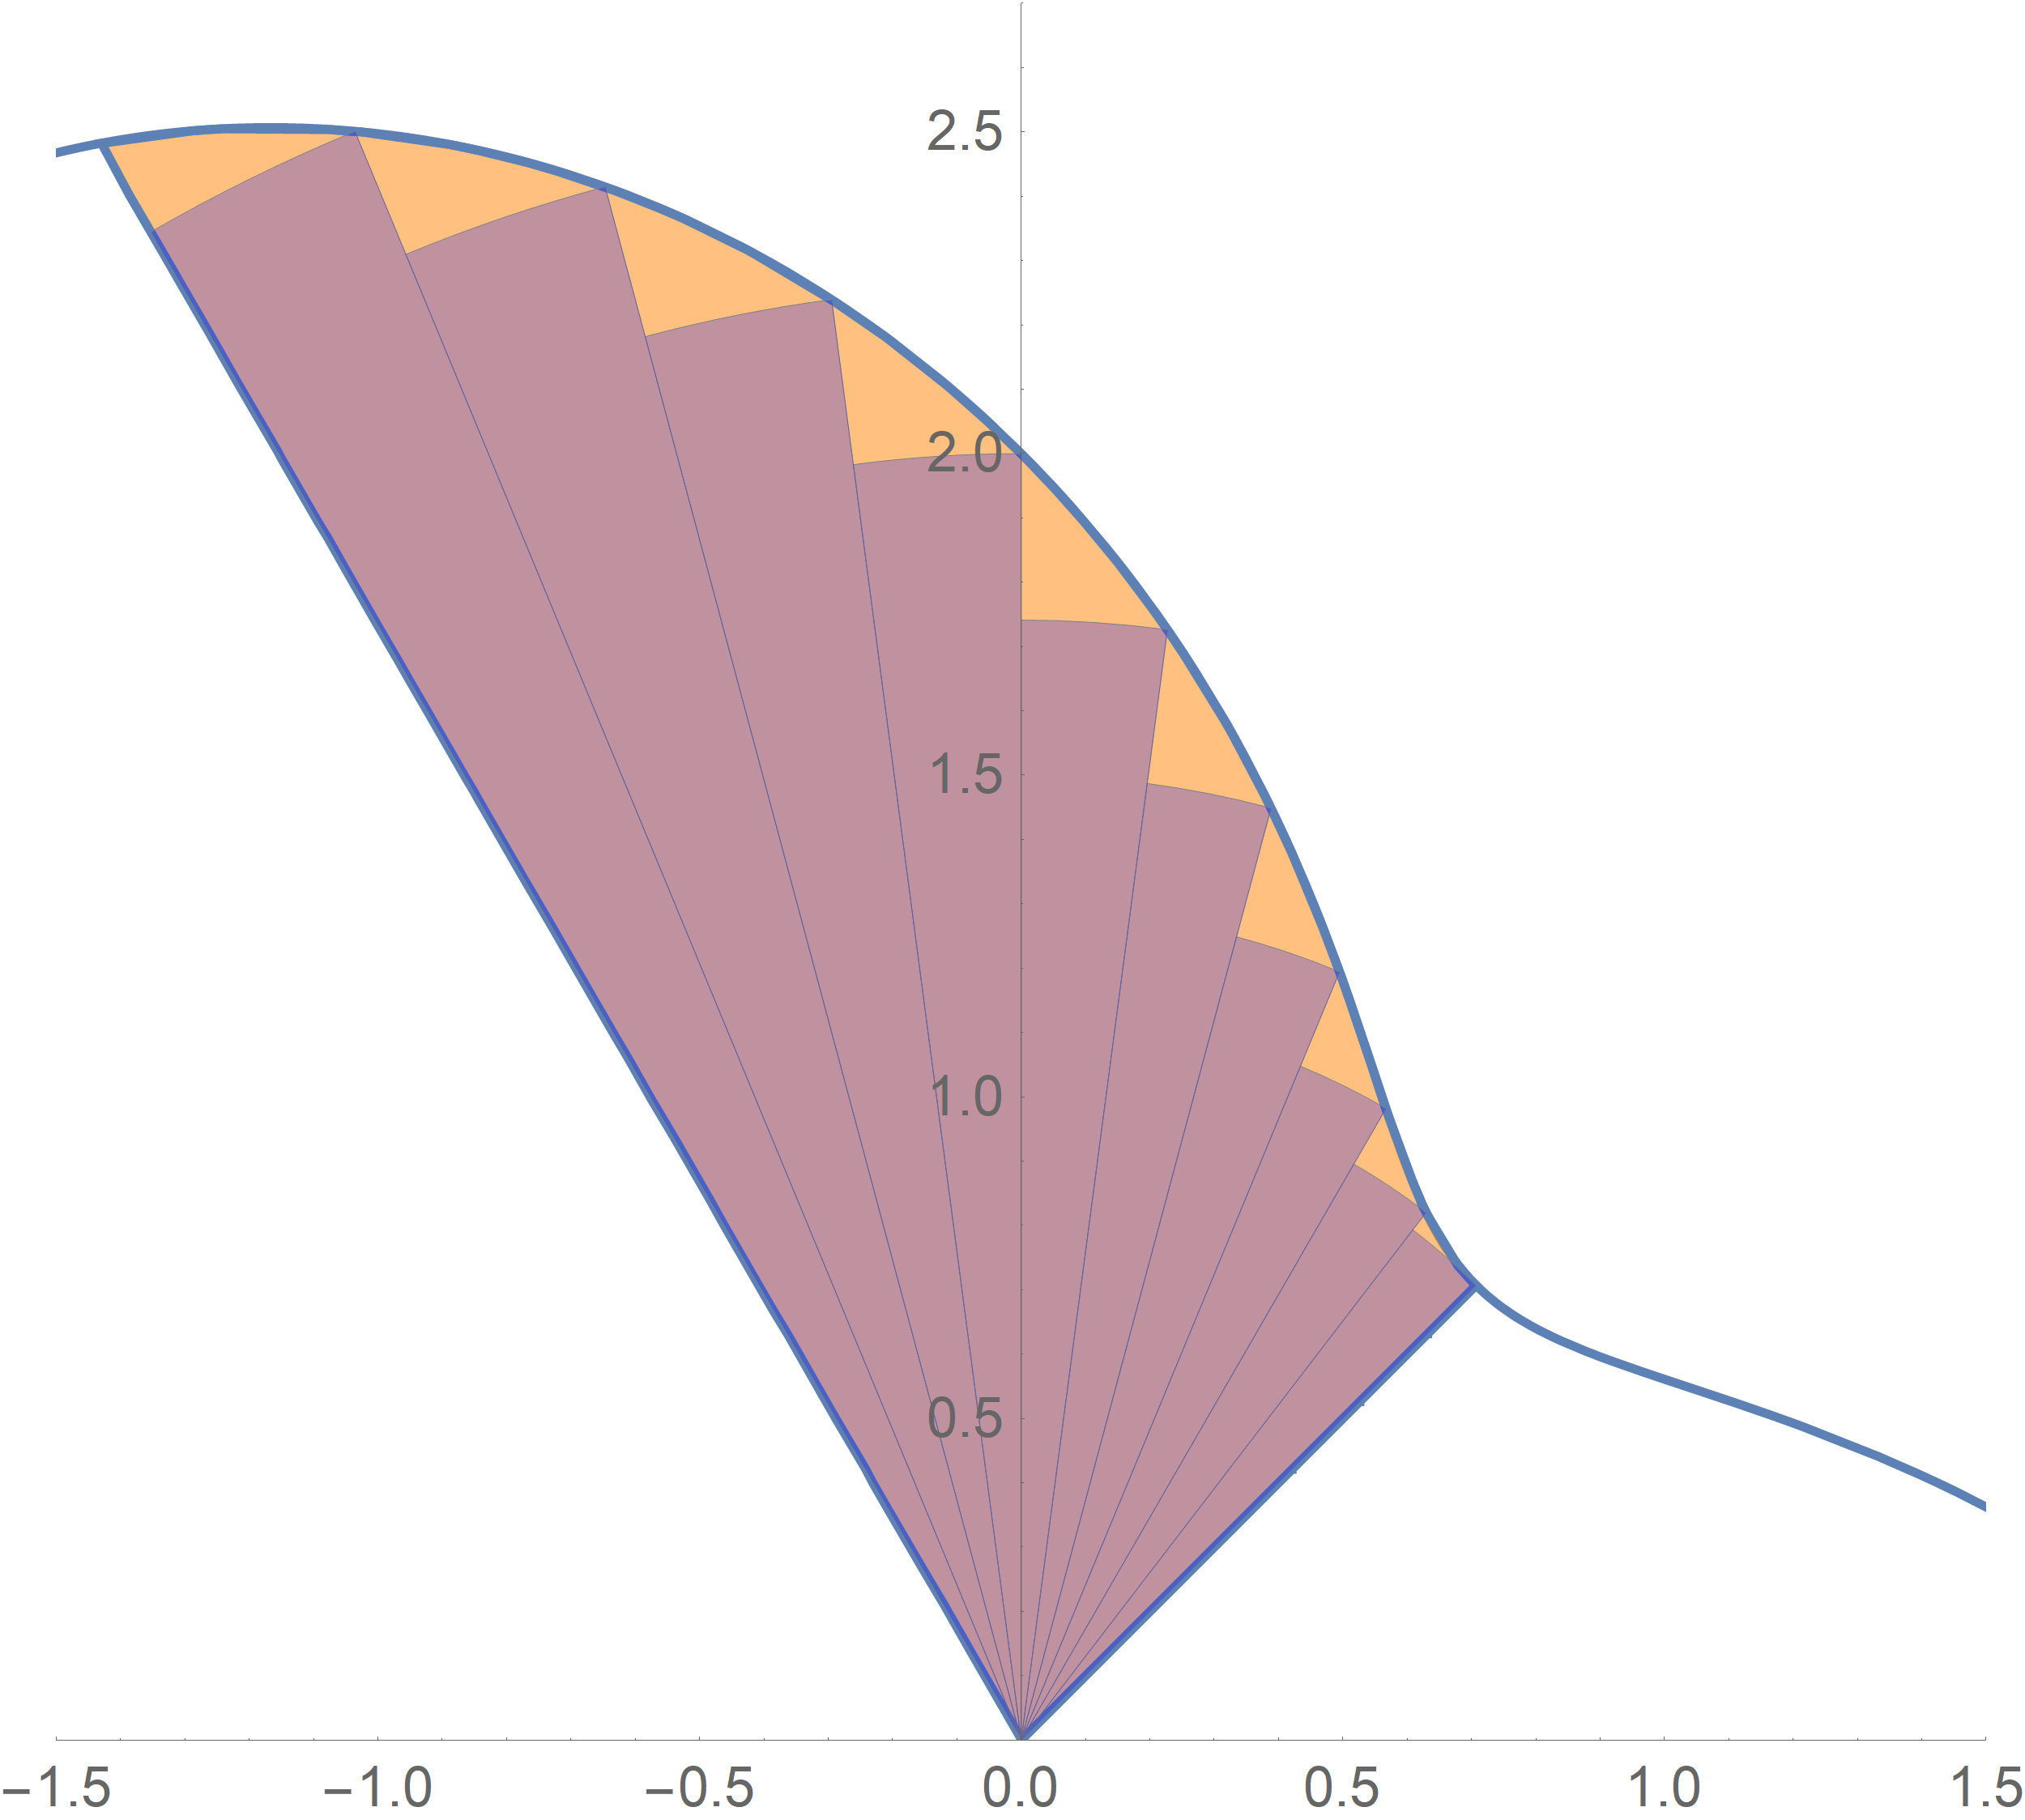
\includegraphics[width=0.4\textwidth]{Figures/polarrects.png}
    \caption{Setup of area of polar region.}
    \label{f:polarrects}
\end{figure}

\begin{example}\label{e:polararearecip}
    Find the area bounded by the graph of $r = \frac{1}{\theta}, \pi \leq \theta \leq 2\pi$.
    \begin{solution}
        \[A = \int_{\pi}^{2\pi} \left( \frac{1}{\theta} \right)^{2} \, d\theta = -\frac{1}{\theta}\bigg|_{\pi}^{2\pi} = \frac{1}{4\pi}\]
    \end{solution}
\end{example}

\begin{example}\label{e:polarbetween}
    Find the area bounded between the graphs of $r = 1 - \cos \theta$ and $r = 2 + \cos \theta$.
    \begin{solution}
        The region is shown in Figure \ref{f:polarbetween}. Note that with the identity $\cos (-\theta) = \cos \theta$ we have symmetry about the $x$-axis, saving a little work. \faSmile

        First find where they intersect: $1 - \cos \theta = 2 + \cos \theta \Rightarrow \theta = \frac{2\pi}{3}, \frac{4\pi}{3}$. Now using symmetry we have
        \begin{align*}
            A   &= 2\left( \frac{1}{2} \int_{0}^{2\pi/3}\left( 1 - \cos \theta \right)^{2} d\theta + \int_{2\pi/3}^{\pi} \left( 2 + \cos \theta \right)^{2} d\theta  \right)\\
                &= \int_{0}^{2\pi/3} \left( \frac{3}{2} - 2\cos \theta + \frac{1}{2}\cos 2\theta \right) d\theta + \int_{2\pi/3}^{\pi} \left( \frac{9}{2} + 4 \cos \theta + \frac{1}{2} \cos 2\theta \right) \, d\theta\\
                &= \frac{5\pi}{2} - 3\sqrt{3}
        \end{align*}
    \end{solution}
    \begin{figure}[htbp]
        \centering
            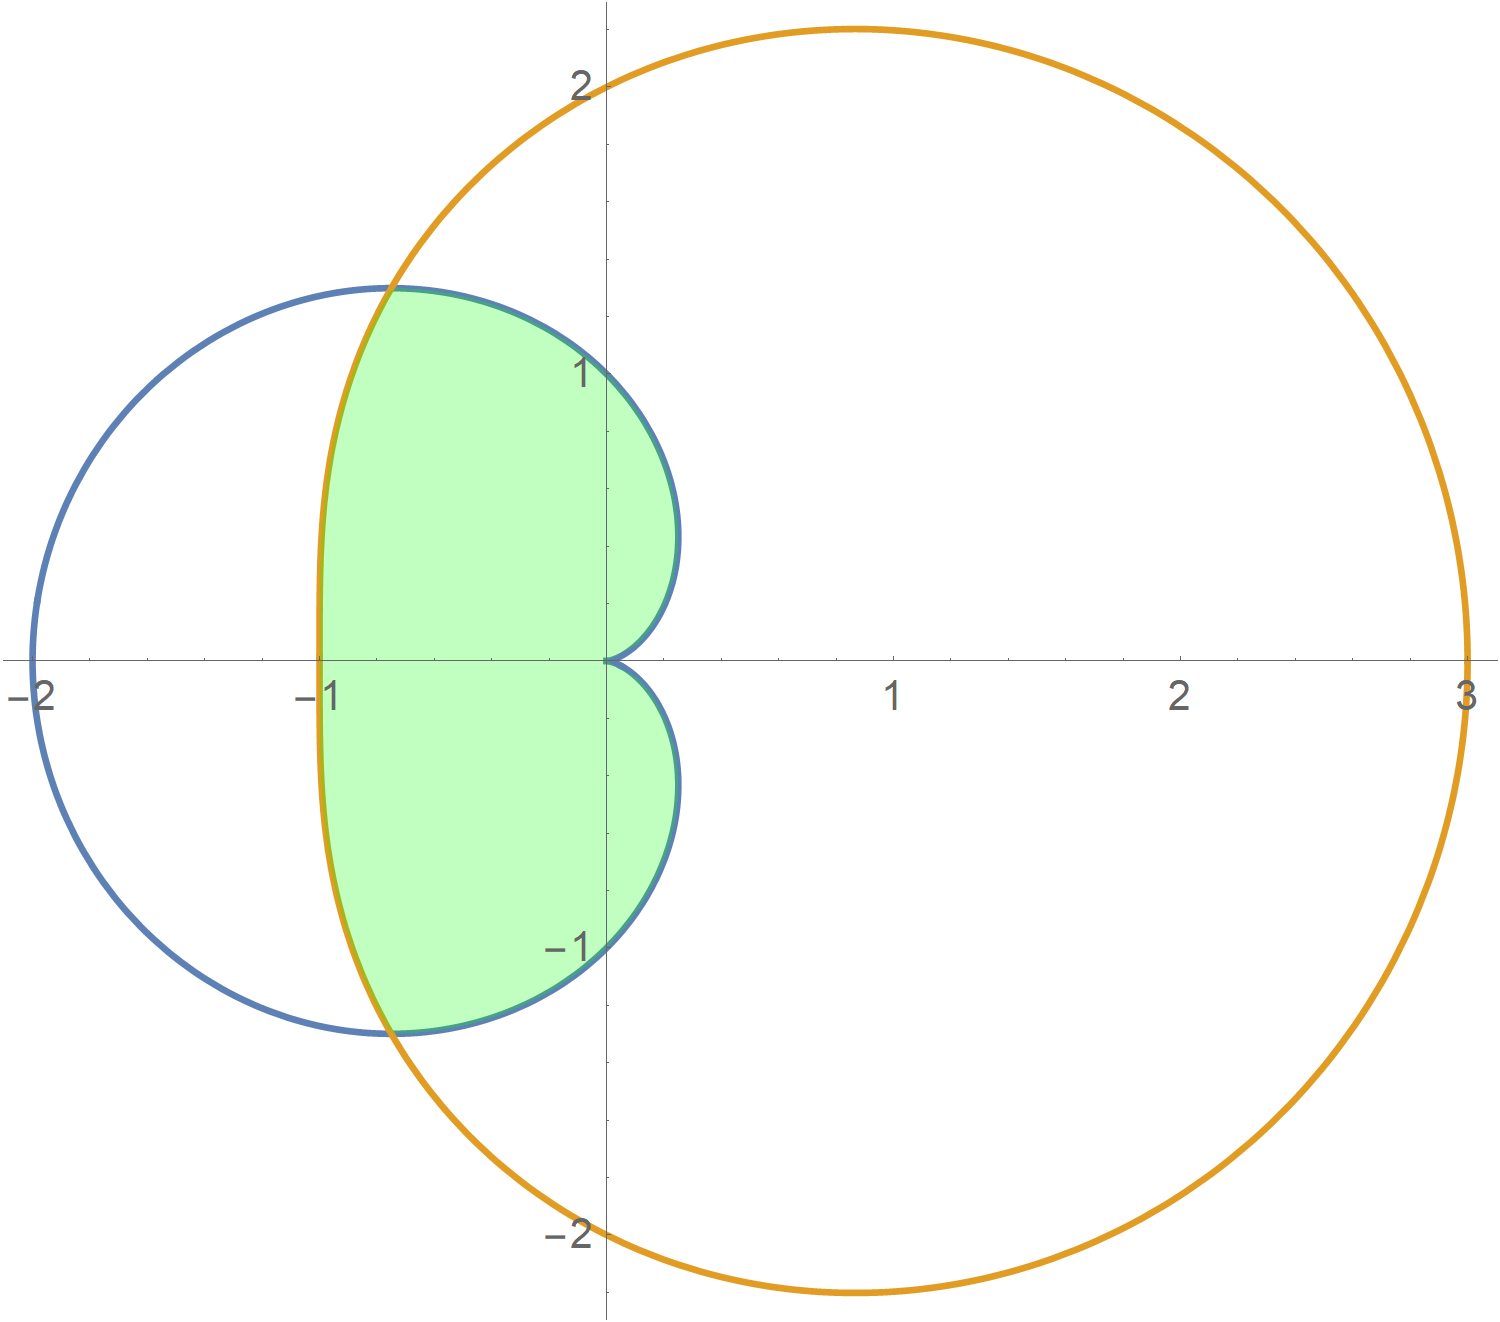
\includegraphics[width=0.4\textwidth]{Figures/polarbetween.png}
        \caption{Region in Example \ref{e:polarbetween}.}
        \label{f:polarbetween}
    \end{figure}
\end{example}

\subsection{Arc Length of Polar Functions}
\begin{itemize}
    \item Follows from parametric curve arc length
    \item Simplified with Pythagorean Identities but derivation is messy and omitted
    \[L = \int_{a}^{b} \sqrt{[f(\theta)]^{2} + [f'(\theta)]^{2}} d\theta\]
\end{itemize}

\begin{example}\label{e:polarlength}
    Find the length along the polar curve $r = 1 + \cos \theta, 0 \leq \theta \leq \frac{\pi}{2}$.
    
    \begin{solution}
        Squaring both $r$ and $r'$ then using a Pythagorean Identity we get
        \[L = \int_{0}^{\pi/2} \sqrt{1 + 2 \cos \theta + \cos^{2} \theta + \sin^{2} \theta}\, d\theta = \int_{0}^{\pi/2} \sqrt{2 + 2\cos \theta} \,d\theta\]
    
    Two ways to go from here. Here is the hard way first! \faSmile \ Start by rationalizing:
    \[\frac{\sqrt{2 + 2\cos \theta}}{1} \cdot \frac{\sqrt{2 - 2\cos \theta}}{\sqrt{2 - 2\cos \theta}} = \frac{\sqrt{2}\sin \theta}{\sqrt{1 - \cos \theta}}\]
    Now we use the substitution $u = 1 - \cos \theta \Rightarrow du = \sin \theta \, d\theta$, $u(\pi/2) = 1, u(0) =  0$ to get
    \[L = \sqrt{2} \int_{0}^{1} u^{-1/2} \, du = 2\sqrt{2}\]
    Note that this is technically an improper integral but it is one we have seen before and it is convergent.

    The method above works more generally (e.g. if we had $\sqrt{2 + 2 \sin \theta}$ we would need to do the above), but for this particular example we have a shortcut. Note that we have the half-angle identity $\cos^{2} \left( \frac{\theta}{2} \right) = \frac{1}{2} + \frac{1}{2} \cos \theta \Rightarrow 2 + 2\cos \theta = 4\cos^{2} \left( \frac{\theta}{2} \right)$ so we actually have a nice perfect square under the radical! \faSmile \ Now we take

    \begin{align*}
        \int_{0}^{\pi/2} \sqrt{2 + 2\cos \theta} \,d\theta  &= \int_{0}^{\pi/2} \sqrt{4\cos^{2} \left( \frac{\theta}{2} \right)}\, d\theta \\
                                                            &= \int_{0}^{\pi/2} 2\cos \left( \frac{\theta}{2} \right)\, d\theta \\
                                                            &= 2\sqrt{2}.
    \end{align*}
    Note that since we are integrating in the interval $\left[ 0, \frac{\pi}{2}\right]$, $\cos \frac{\theta}{2} > 0$ so we need not worry about absolute values when evaluating the square root.
    \end{solution}
\end{example}

\section{Conic Sections}
\setcounter{figure}{0}
\subsection{Common Definition}
\begin{itemize}
    \item A \textbf{conic section} is the curve we get by cutting a right circular cone with a plane
    \item Can be a circle, ellipse, parabola, or hyperbola
    \item Figures below show how!
    \item Only dealing with conics centered at origin
    \item We will either use information about conic to get equation or vice-versa
    \item[\faThumbsUp] It helps a lot if you plot/graph as you go to visualize
\end{itemize}
\begin{figure}[htbp]
    \centering
    \begin{minipage}{0.45\textwidth}
        \centering
        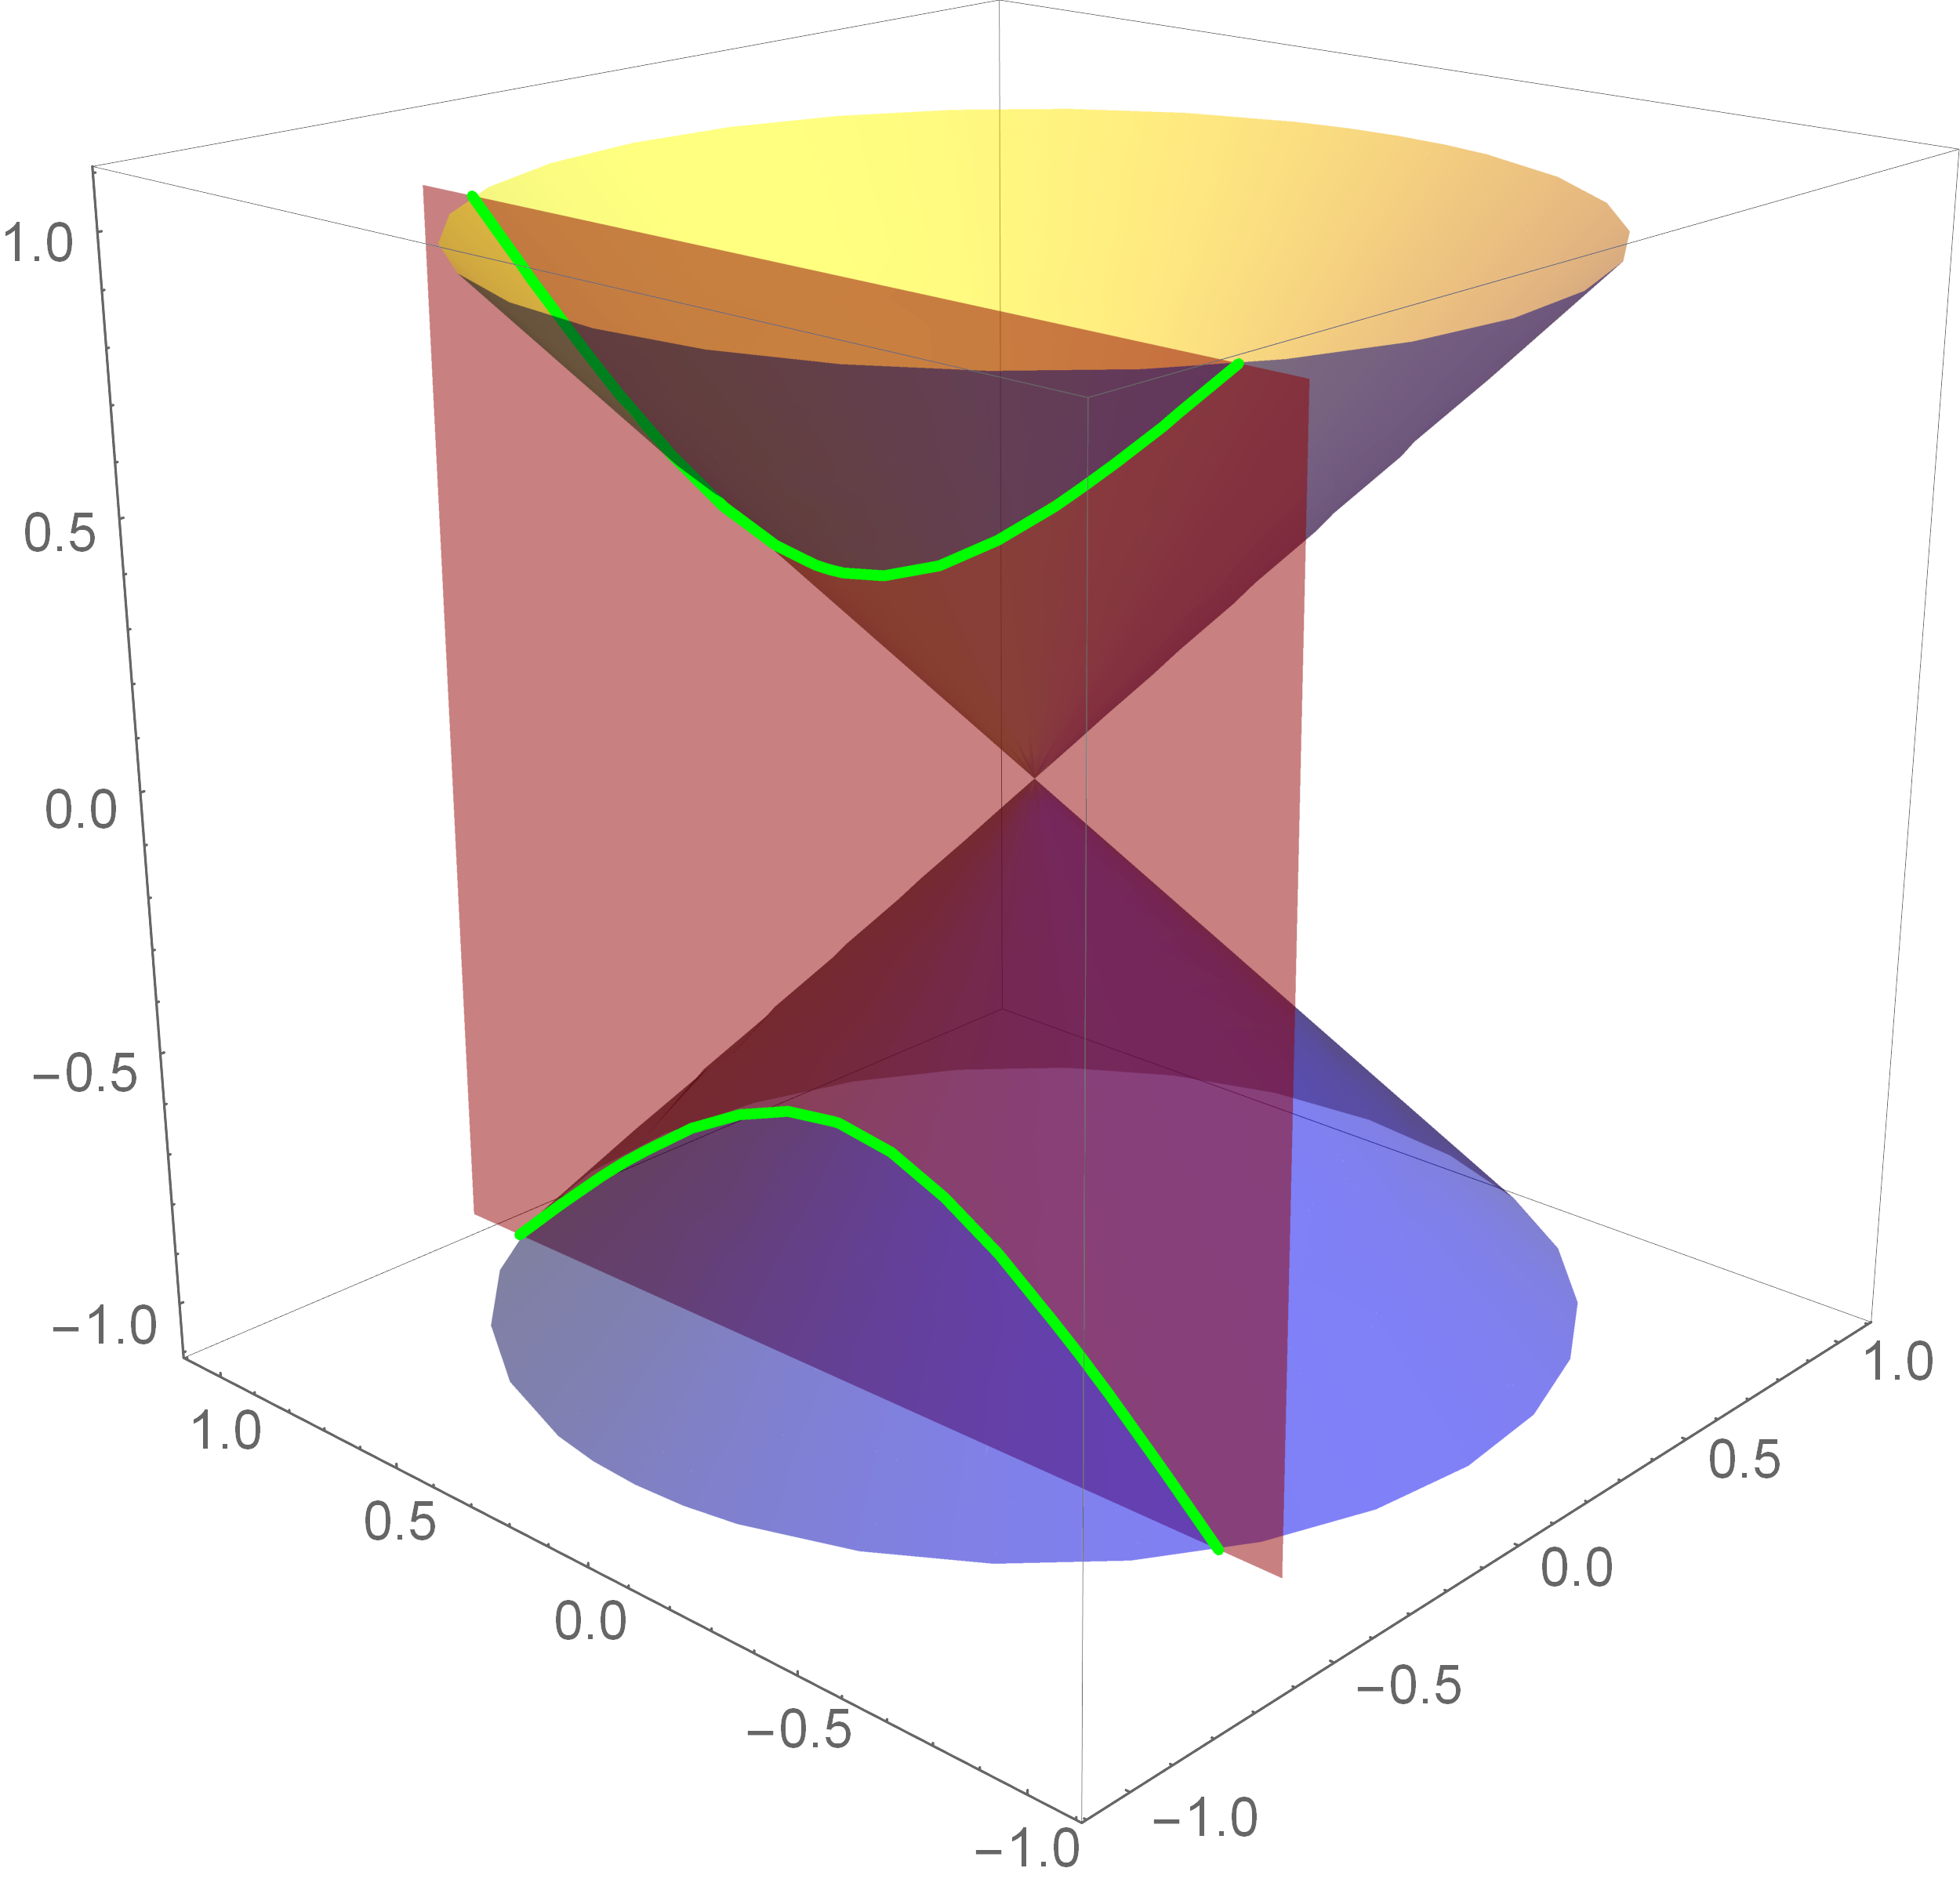
\includegraphics[width=0.9\textwidth]{Figures/conichyperbola.png}
        \caption{Plane intersecting with a cone to form a hyperbola.}
        \label{f:conichyperbola}
    \end{minipage}\hfill
    \begin{minipage}{0.45\textwidth}
        \centering
        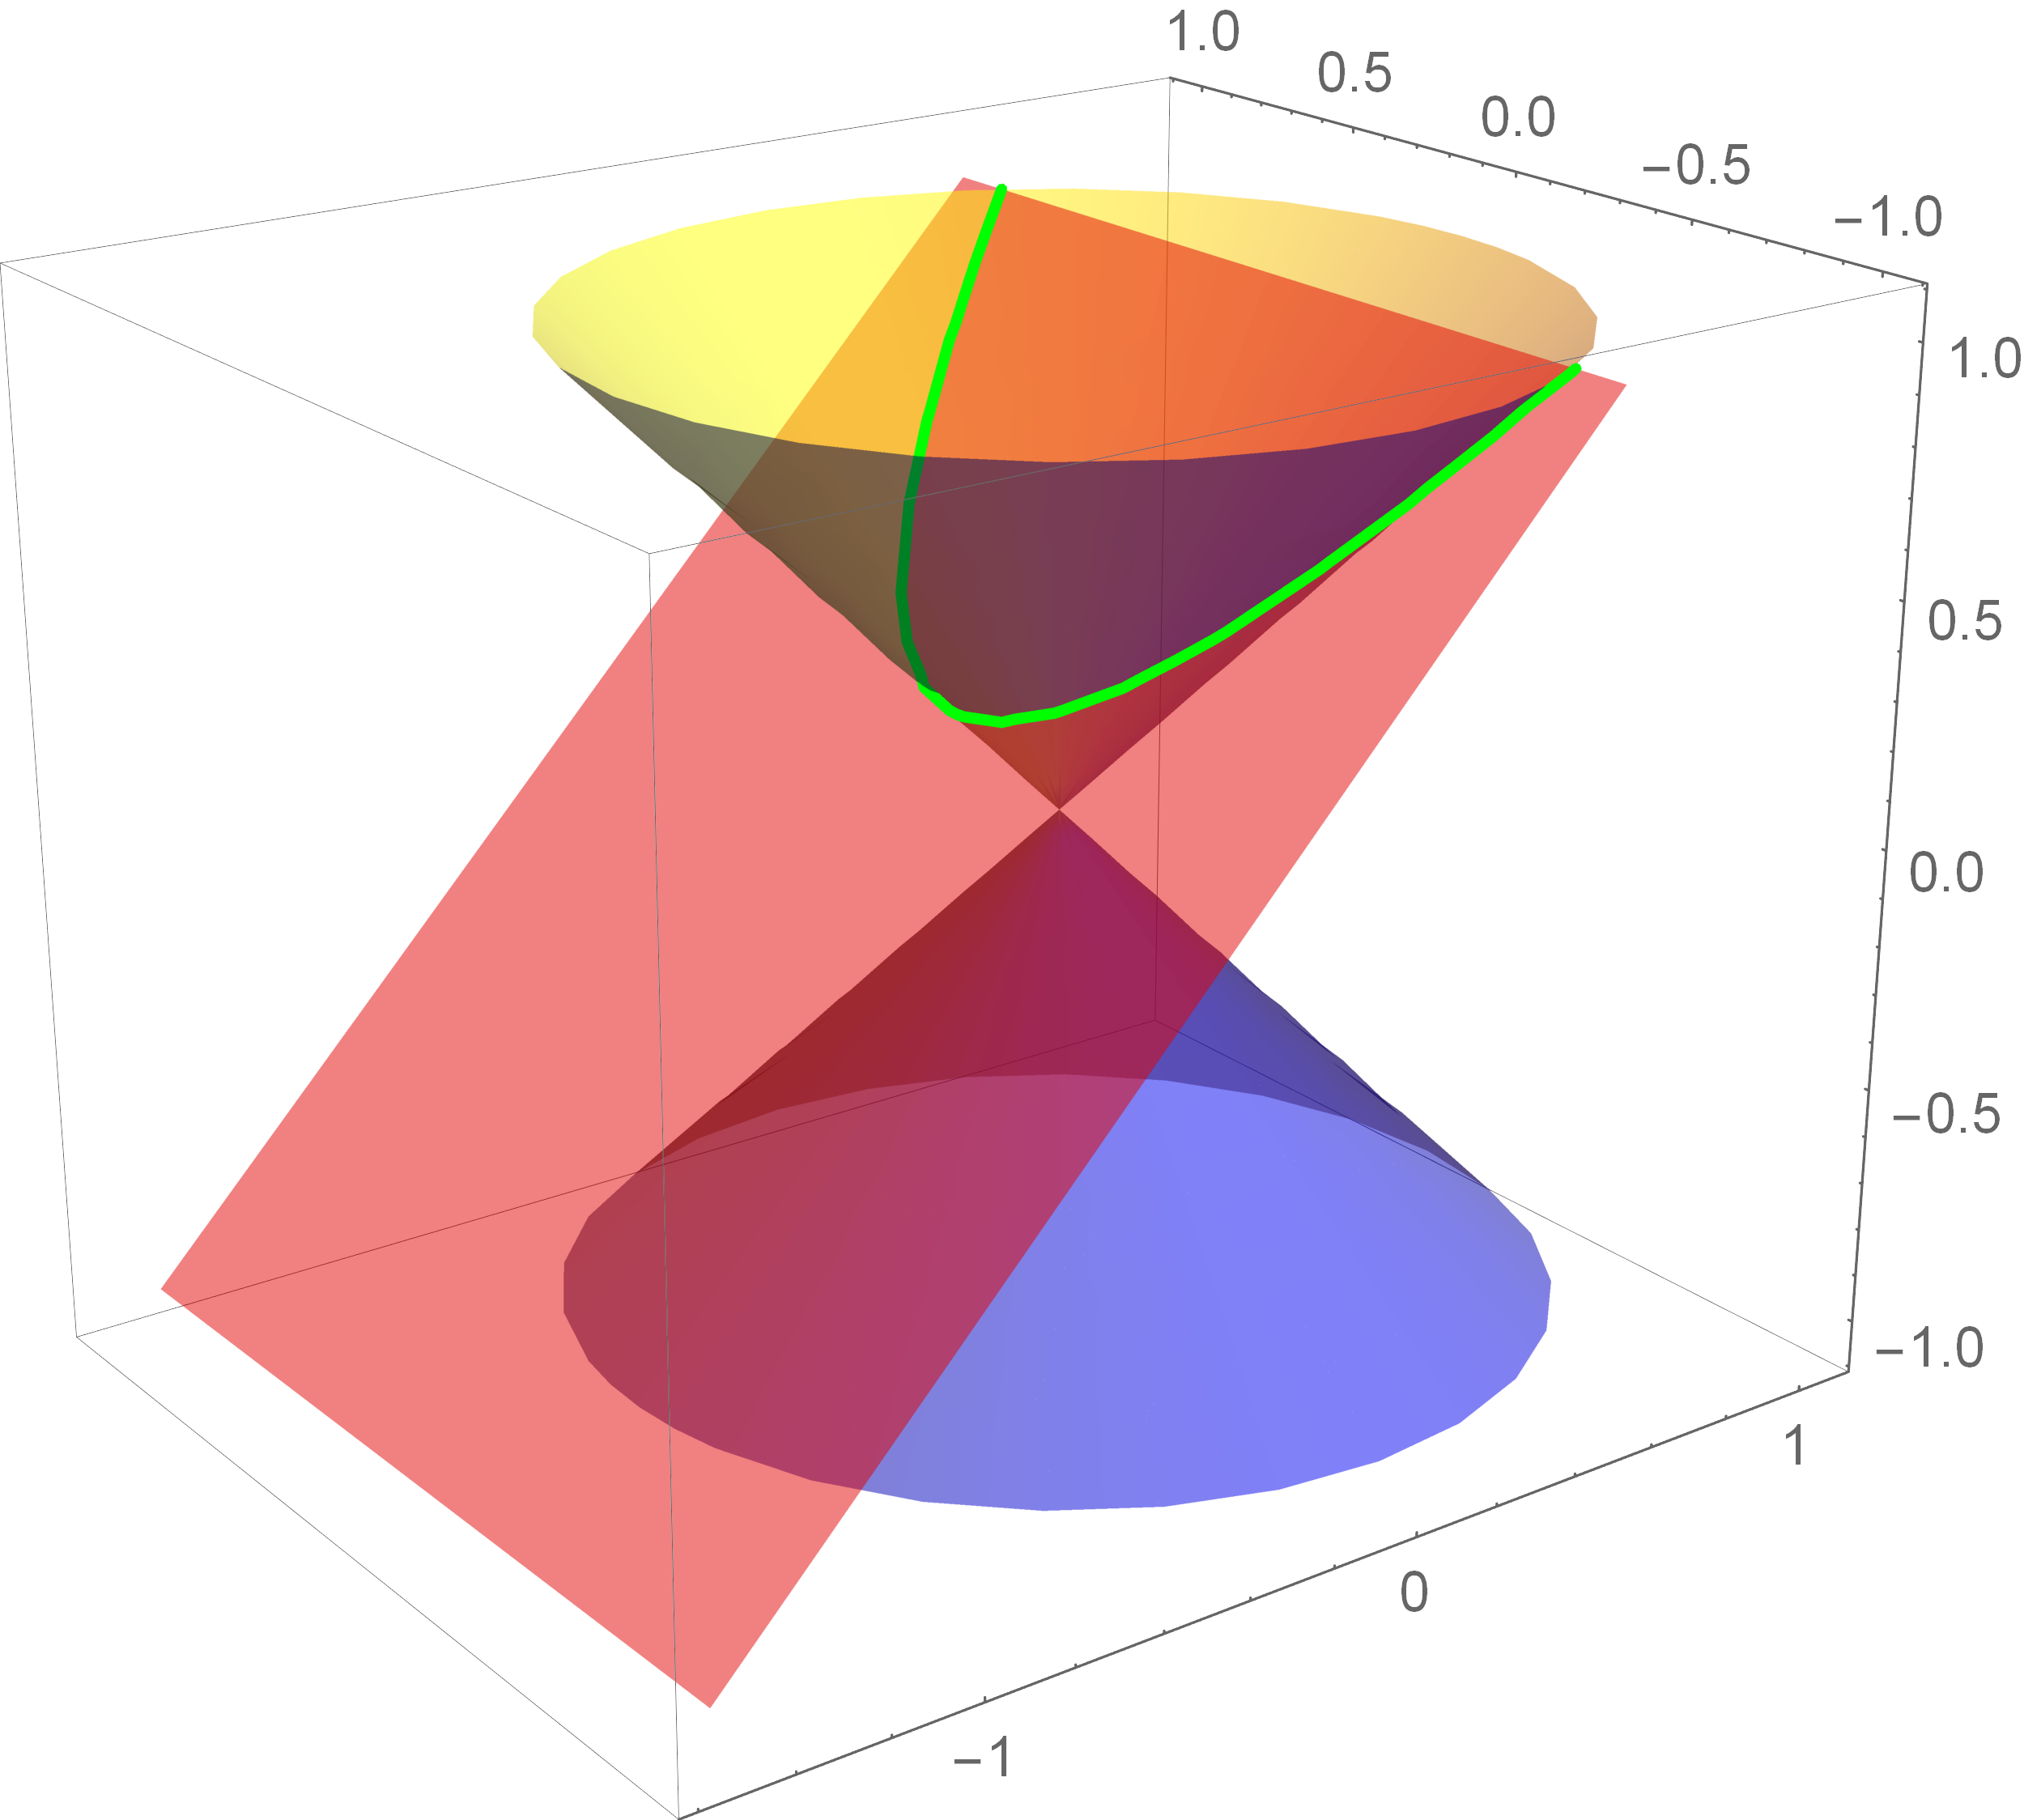
\includegraphics[width=0.9\textwidth]{Figures/conicparabola.png}
        \caption{Plane intersecting with a cone to form a parabola.}
        \label{f:conicparabola}
    \end{minipage}\hfill
\end{figure}

\begin{figure}[htbp]
    \centering
    \begin{minipage}{0.45\textwidth}
        \centering
        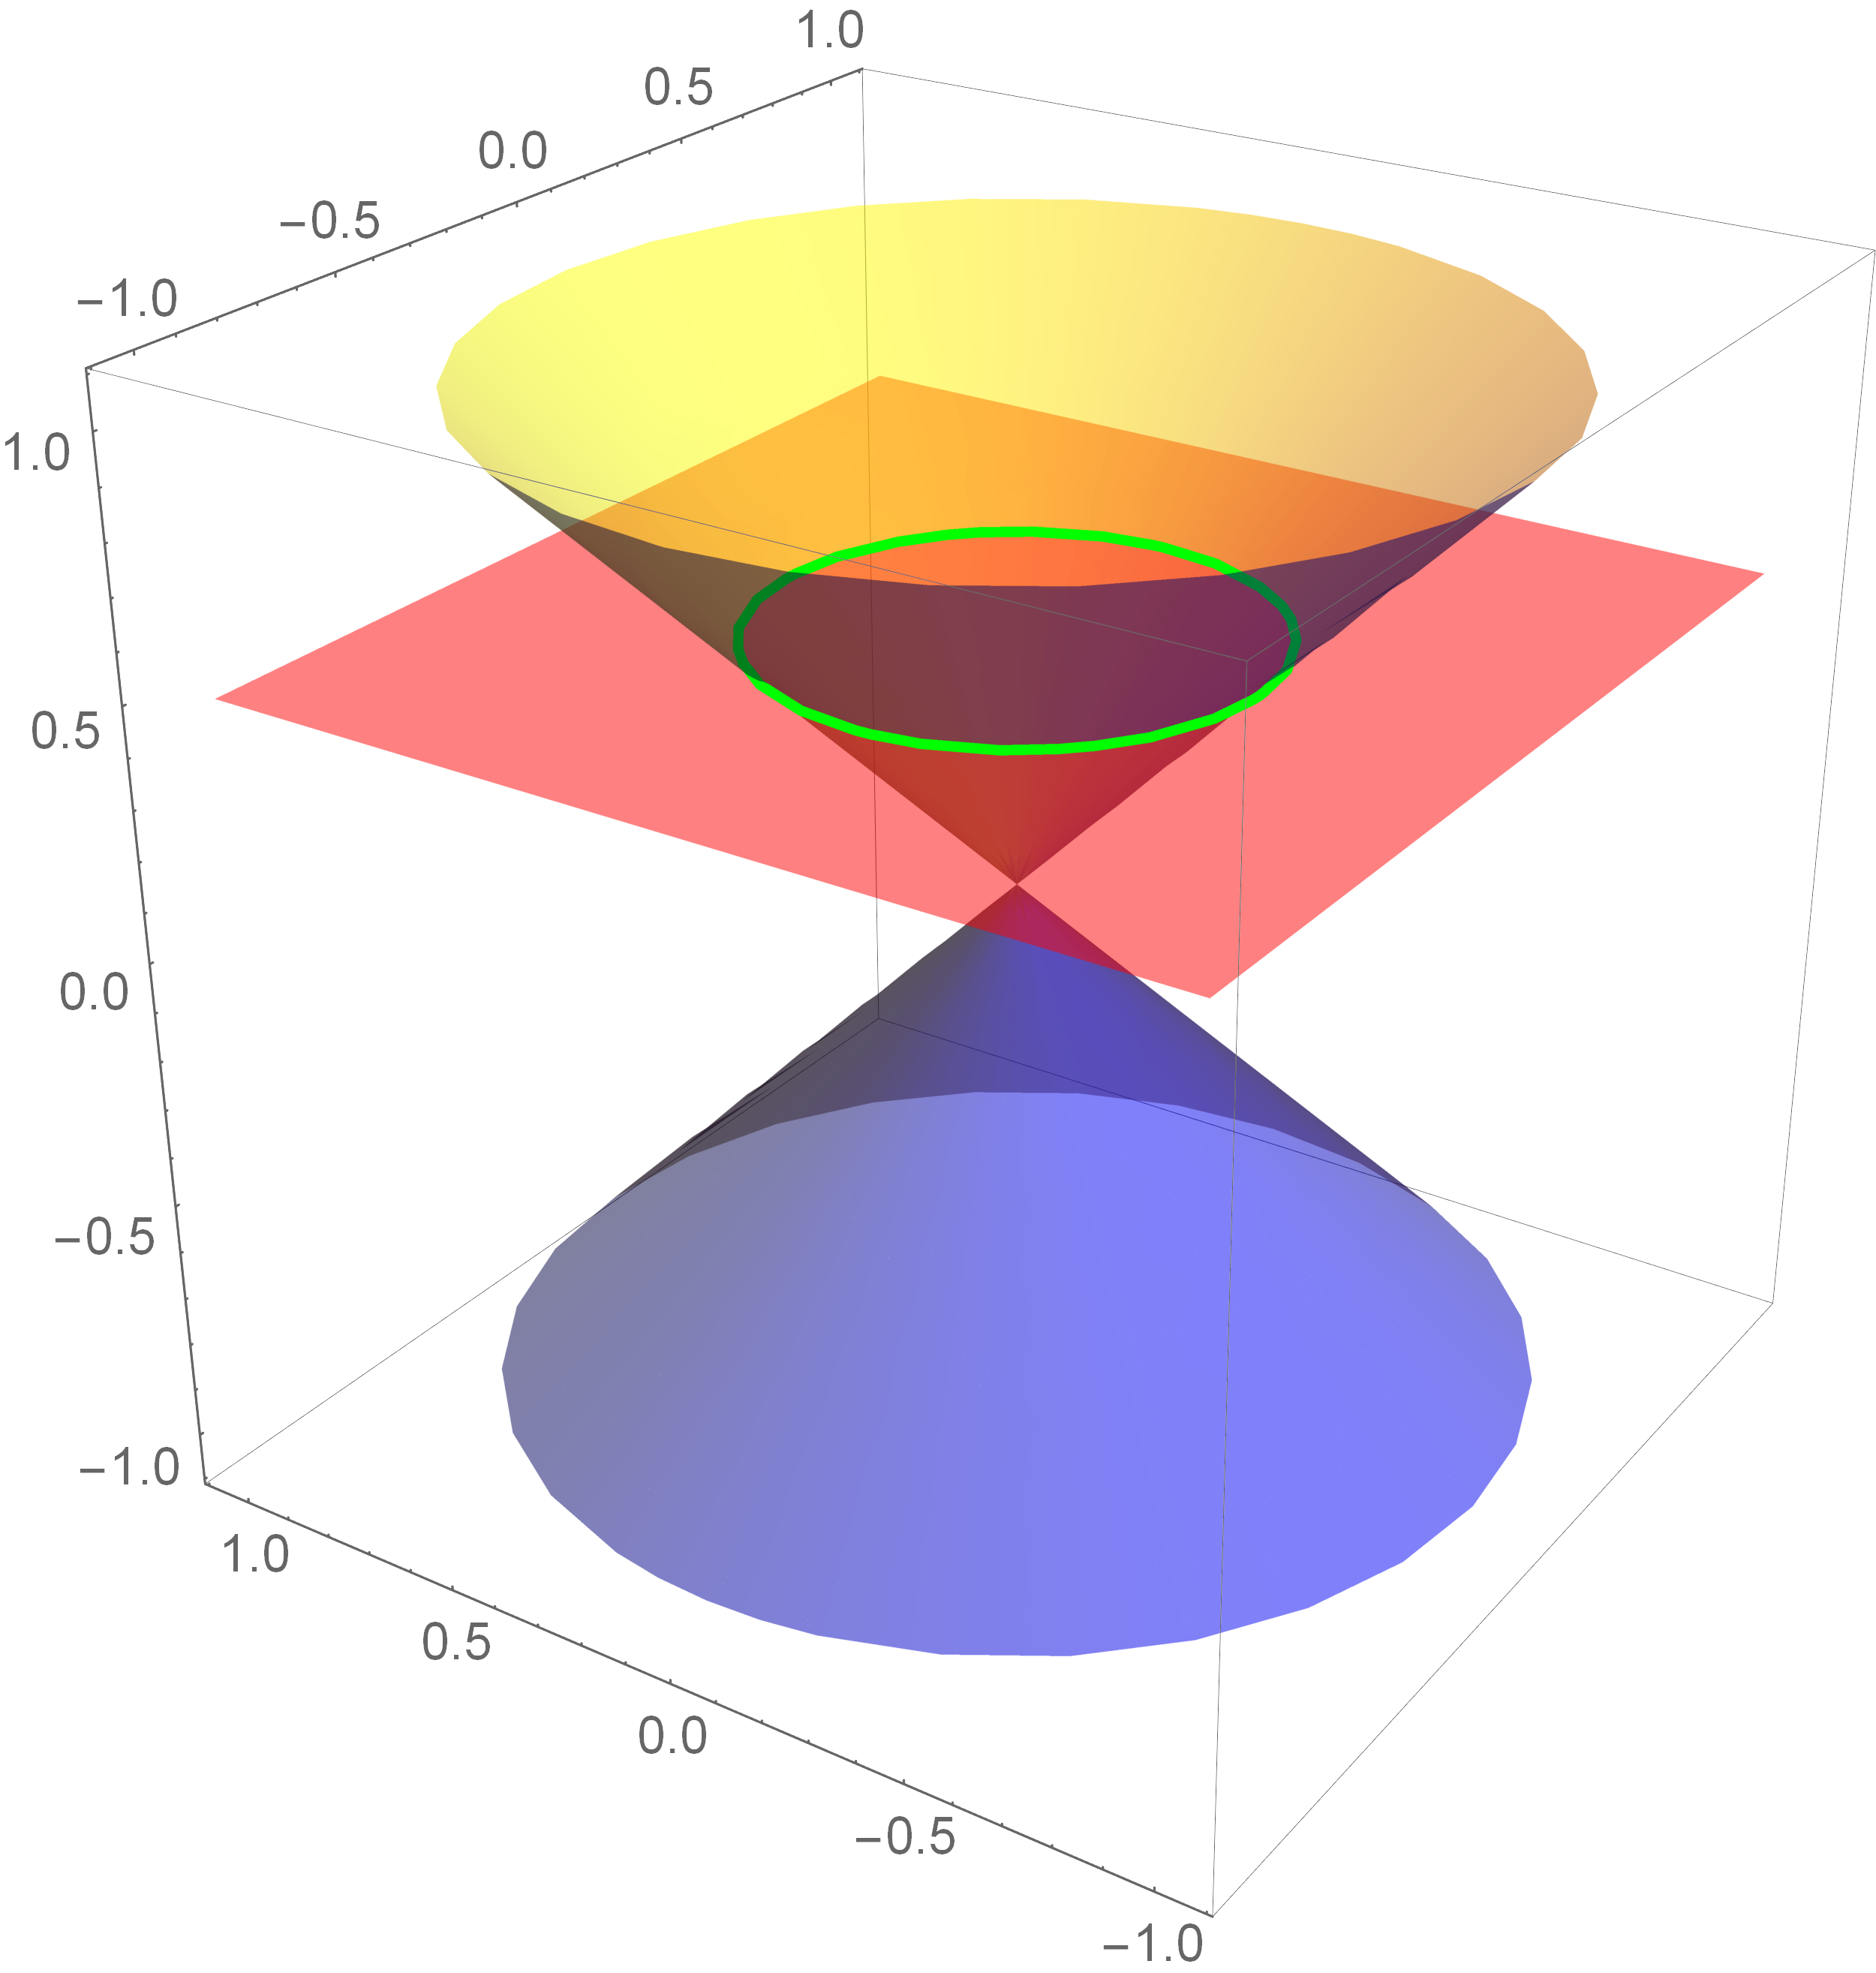
\includegraphics[width=0.9\textwidth]{Figures/coniccircle.png}
        \caption{Plane intersecting with a cone to form a circle.}
        \label{f:coniccircle}
    \end{minipage}\hfill
    \begin{minipage}{0.45\textwidth}
        \centering
        \includegraphics[width=0.9\textwidth]{Figures/conicellipse.png}
        \caption{Plane intersecting with a cone to form an ellipse.}
        \label{f:conicellipse}
    \end{minipage}\hfill
\end{figure}

\subsection{Parabolas}
\begin{itemize}
    \item A \textbf{parabola} is the set of points that are equally distant from a fixed point (the \textbf{focus}) and a fixed line (the \textbf{directrix}).
    \item The \textbf{vertex} is the point where the parabola makes its U-turn
    \item The \textbf{axis} is the line containing the focus and vertex
    \begin{itemize}
        \item Note that axis is perpendicular to directrix
    \end{itemize}
    \item Start with parabola opening up (See Figure \ref{f:paraboladef})
    \begin{itemize}
        \item Pick generic point $P(x,y)$ on parabola
        \item Focus at point $F(0,c) \Rightarrow$ directrix is $y = -c$
        \item Now set distances from $P$ to $F$ and $P$ to $D$ equal. Note we can just set squares of distances equal to avoid roots \faSmile
        \begin{align*}
            (x-0)^{2} + (y-c)^{2} &= (x-x)^{2} + (y+c)^{2}\\
            x^{2} + y^{2} -2cy + c^{2} &= y^{2} + 2cy + c^{2}\\
            x^{2} &= 4cy
        \end{align*}
        \item If $c < 0$ parabola is facing down
    \end{itemize}
    \item Parabola facing right? Similar derivation $y^2 = 4cx, c > 0$; faces left if $c < 0$
\end{itemize}

\begin{figure}[htbp]
    \centering
        \includegraphics[width=0.6\textwidth]{Figures/paraboladef.pdf}
    \caption{Parabola opening upward with vertex at the origin.}
    \label{f:paraboladef}
\end{figure}

\begin{example}\label{e:parabolaleft}
    Find the equation of the parabola with focus $(-3, 0)$ and directrix $x = 3$.
    \begin{solution}
        Note that positions of focus and directrix imply vertex at the origin. Here $c = -3$ and directrix is vertical line; equation is $y^2 = -12x$. A graph is shown in Figure \ref{f:parabolaleft}.
    \end{solution}
\end{example}

\begin{figure}[htbp]
    \centering
        \includegraphics[width=0.4\textwidth]{Figures/parabolaleft.pdf}
    \caption{Parabola and directrix from Example \ref{e:parabolaleft}.}
    \label{f:parabolaleft}
\end{figure}

\begin{example}\label{e:paraboladown}
    Find the directrix and focus of the parabola $y = -\frac{1}{10}x^{2}$.
    \begin{solution}
        This is a parabola with its vertex at the origin; with the $x$ term squared we know it opens either up or down; here $c = -\frac{5}{2}$ so it opens down. The directrix is the line $y = \frac{5}{2}$ and the focus is at $(0, -\frac{5}{2})$. A graph is shown in Figure \ref{f:paraboladown}.
    \end{solution}
\end{example}

\begin{figure}[htbp]
    \centering
        \includegraphics[width=0.4\textwidth]{Figures/paraboladown.pdf}
    \caption{Parabola and directrix from Example \ref{e:paraboladown}.}
    \label{f:paraboladown}
\end{figure}

\subsection{Ellipses}
\begin{itemize}
    \item An \textbf{ellipse} is the set of points for which the sum of the distances to two fixed points (the \textbf{foci}) is constant
    \item Has a \textbf{major axis} (longer) and \textbf{minor axis}
    \item \textbf{Vertices} and foci are all along major axis
    \item Centered at origin; if $a$ is the distance from the center to either vertex, vertices at $(\pm a, 0)$
    \item $c$ is distance from center to either focus; foci at $(\pm c, 0)$
    \item $b$ is the distance from center to point on ellipse on minor axis
    \item For all ellipses, $a > b > 0$ and $c^{2} = a^{2} - b^{2}$
    \item Derivation of equation messy, but if ellipse centered at origin and horizontal major axis (as in Figure \ref{f:ellipsedef}) has the equation
    \[\frac{x^{2}}{a^{2}} + \frac{y^{2}}{b^{2}} = 1\]
    \item If vertical axis:
    \[\frac{y^{2}}{a^{2}} + \frac{x^{2}}{b^{2}} = 1\]
\end{itemize}

\begin{figure}[htbp]
    \centering
        \includegraphics[width = 0.4\textwidth]{Figures/ellipsedef.pdf}
    \caption{Ellipse centered at origin with horizontal major axis.}
    \label{f:ellipsedef}
\end{figure}

\begin{example}\label{e:ellipse-eqn}
    Find an equation of the ellipse with foci $(\pm 4, 0)$ and through the points $(0, \pm 6)$ then sketch.
    \begin{solution}
        With the foci centered at the origin we know the center of the ellipse is there and $c = 4$. This also shows that the major axis is horizontal. The two points on the ellipse are also symmetric about the origin and the line segment joining them is perpendicular to the major axis so they are the point on the ellipse on the minor axis so web know $b = 6$. Now $4^{2} = a^{2} - 6^{2} \Rightarrow a = \sqrt{52}$. So the equation is $\displaystyle \frac{x^{2}}{52} + \frac{y^{2}}{36} = 1$. The graph is show in Figure \ref{f:ellipse-eqn}.
    \end{solution}
\end{example}

\begin{example}
    Find an equation of the ellipse with vertices $(0, \pm 8)$ and through the point $P\left( \frac{\sqrt{3}}{2}, 4 \right)$.
    \begin{solution}
        The origin is the midpoint between the vertices so we know the center is at the origin, the major axis is vertical, and that $a = 8$. So the equation starts off as
        \[\frac{y^{2}}{64} + \frac{x^{2}}{b^{2}}  = 1\]
        so we plug in the coordinates of the given point $P$ to get $\displaystyle \frac{1}{4} + \frac{3}{4b^{2}} = 1 \Rightarrow b = 1$ so the equation is
        \[\frac{y^{2}}{64} + x^{2}  = 1.\]
    \end{solution}
\end{example}

\begin{figure}[htbp]
    \centering
        \includegraphics[width=0.4\textwidth]{Figures/ellipseeqn.pdf}
    \caption{Graph of ellipse in Example \ref{e:ellipse-eqn}.}
    \label{f:ellipse-eqn}
\end{figure}

\begin{example}\label{e:ellipseinfo}
    Find the foci and vertices of the ellipse $36x^{2} + 4y^{2} = 144$.
    \begin{solution}
        First get the equation in the right form: $\displaystyle \frac{x^{2}}{4} + \frac{y^{2}}{36} = 1$. The $y^{2}$ term has the greater denominator so the ellipse has a vertical axis and $a = 6, b = 2 \Rightarrow c = 4\sqrt{2}$. The vertices are at $(0, \pm 6)$ and foci at $(0, 4\sqrt{2})$. The graph is shown in Figure \ref{f:ellipseinfo}.
    \end{solution}
\end{example}

\begin{figure}[htbp]
    \centering
        \includegraphics[width=0.15\textwidth]{Figures/ellipseinfo.pdf}
    \caption{Graph of ellipse in Example \ref{e:ellipseinfo}.}
    \label{f:ellipseinfo}
\end{figure}

\subsection{Hyperbolas}
\begin{itemize}
    \item A \textbf{hyperbola} is the set of points for which the absolute value of the difference of the distances to two fixed points (the \textbf{foci}) is constant
    \item Vertices and foci are on the axis
    \item Branches of the hyperbola follow asymptotes; see Figure \ref{f:hyperboladef}
    \item As with ellipses $a$ is the distance from the center to either vertex
    \item $c$ is the distance from the center to either focus
    \item $b$ is the shortest distance from a vertex to an asymptote in direction perpendicular to the axis
    \item For all hyperbolas, $c^{2} = a^{2} + b^{2}$
    \item Asymptote equations if center at origin:
    \begin{itemize}
        \item Horizontal axis: $y = \pm \frac{b}{a} x$
        \item Vertical axis: $y = \pm \frac{a}{b} x$
    \end{itemize}
    \item For horizontal axis: $\displaystyle \frac{x^{2}}{a^{2}} - \frac{y^{2}}{b^{2}} = 1$
    \item For vertical axis: $\displaystyle \frac{y^{2}}{a^{2}} - \frac{x^{2}}{b^{2}} = 1$
    \begin{itemize}
        \item If confused, try plugging in $x=0$ or $y=0$ and see if the result makes sense
    \end{itemize}
\end{itemize}

\begin{figure}[htbp]
    \centering
        \includegraphics[width = 0.4\textwidth]{Figures/hyperboladef.pdf}
    \caption{Hyperbola centered at the origin with a horizontal axis.}
    \label{f:hyperboladef}
\end{figure}

\begin{example}\label{e:hyperbolaeqn}
    Find the foci and asymptotes of the hyperbola $25x^{2} - 4y^{2} = 100$ and sketch.
    \begin{solution}
        First get in standard form: $\displaystyle \frac{x^{2}}{4} - \frac{y^{2}}{25} = 1$; now the $x^{2}$ term is positive so the axis is horizontal. So here $a = 2$ and $b = 5$ so the asymptotes are $y = \pm \frac{5}{2}x$. For the foci $c^2 = 2^{2} + 5^{2} = 29  \Rightarrow c = \sqrt{29}$ and the foci are at $(\pm \sqrt{29}, 0)$. A graph is shown in Figure \ref{f:hyperbolaeqn}.
    \end{solution}
\end{example}

\begin{figure}[htbp]
    \centering
        \includegraphics[width=0.4\textwidth]{Figures/hyperbolaeqn.pdf}
    \caption{Graph of hyperbola with its foci and asymptotes from Example \ref{e:hyperbolaeqn}.}
    \label{f:hyperbolaeqn}
\end{figure}

\begin{example}\label{e:hyperbolaasymp}
    Find an equation of the hyperbola with asymptotes $y = \pm 2x$ and foci $\left(0, \pm 4\sqrt{5}\right)$ then sketch.
    \begin{solution}
        The location of the foci tell us that the axis of the hyperbola is vertical and that $c = 4\sqrt{5}$. Since the axis is vertical, the slope of the asymptotes gives us $\frac{a}{b} = 2 \Rightarrow a = 2b$. We can use this with the equation $c^{2} = a^{2} + b^{2}$ to find $a$ and $b$. Plugging in we get $(4\sqrt{5})^{2} = (2b)^{2} + b^{2} \Rightarrow 80 = 5b^{2} \Rightarrow b = 4 \Rightarrow a = 8$. The equation of the hyperbola is $\displaystyle \frac{y^{2}}{64} - \frac{x^{2}}{16} = 1$. A graph is shown in Figure \ref{f:hyperbolaasymp}.
    \end{solution}
\end{example}

\begin{figure}[htbp]
    \centering
        \includegraphics[width=0.4\textwidth]{Figures/hyperbolaasymp.pdf}
    \caption{Hyperbola, foci, and asymptotes in Example \ref{e:hyperbolaasymp}.}
    \label{f:hyperbolaasymp}
\end{figure}

\subsection{Polar Equations of Conic Sections}

\begin{itemize}
    \item Another way to define a conic: a \textbf{conic} is the set of points for which the ratio of the distance to a fixed point (a \textbf{focus}) to the distance to a fixed line (a \textbf{directrix}) is constant. This ratio is called the \textbf{eccentricity} of the conic, $e$.
    \item Can classify conic by $e$:
    \begin{table}[htbp]
	\centering
	\caption{Conics and their eccentricities}
	\begin{tabular}{cl}
		$\bm{e}$    & \textbf{Conic Type} \\ \hline
		$e = 0$     & Circle \\
		$0 < e < 1$ & Ellipse \\
        $e = 1$     & Parabola \\
		$e > 1$     & Hyperbola \\ \hline
	\end{tabular}
\end{table}
    \item To get a polar equation of a conic we need a focus at the origin. Assume from here on.
    \item Start with a conic opening to the left towards the focus at the origin
    \begin{itemize}
        \item See Figure \ref{f:polarconic}
    \end{itemize}
    \item Let equation of directrix be $x = d$, $d > 0$
    \item Pick a generic point on the conic $(r, \theta)$
    \item $\displaystyle \frac{r}{d - r \cos \theta} = e$
    \item Solving for $r$ we get $\displaystyle r = \frac{ed}{1 + e\cos \theta}$
    \item Similar derivation if opening right with directrix $x = -d$: $\displaystyle r = \frac{ed}{1 - e\cos \theta}$
    \item Opening down with directrix $y = d$: $\displaystyle r = \frac{ed}{1 + e\sin \theta}$
    \item Opening up with directrix $y = -d$: $\displaystyle r = \frac{ed}{1 - e\sin \theta}$
\end{itemize}

\begin{figure}[htbp]
    \centering
        \includegraphics[width = 0.4\textwidth]{Figures/polarconic.pdf}
    \caption{Conic with a focus at the origin.}
    \label{f:polarconic}
\end{figure}

\begin{example}\label{e:conic-polar-ellipse-eq}
    Find the polar equation of an ellipse with $e = \frac{1}{4}$, directrix $y = -2$, and focus at the origin.
    \begin{solution}
        Here $d = 2$ and we use the form $\displaystyle r = \frac{ed}{1 - e\sin \theta}$ to get $\displaystyle r = \frac{\frac{1}{4}\cdot 2}{1 - \frac{1}{4}\sin \theta} = \frac{2}{4 - \sin \theta}$ 
    \end{solution}
\end{example}

\begin{example}\label{e:conic-polar-hyperbola-eccdir}
    Identify the conic type then find the eccentricity and directrix of the conic with polar equation $\displaystyle r = \frac{21}{4 - 7\cos \theta}$.
    \begin{solution}
        We need to get this in the form $\displaystyle r = \frac{ed}{1 - e\cos \theta}$ first:
        \[r = \frac{21}{4 - 7\cos \theta} = \frac{\frac{21}{4}}{1 - \frac{7}{4}\cos \theta}\]
        So now we see $e = \frac{7}{4}$ so the conic is a hyperbola and $ed = \frac{21}{4} \Rightarrow d = 3$. The form of the equation implies this branch of the hyperbola opens to the right so the directrix is $x = -3$.
    \end{solution}
\end{example}

\begin{example}\label{e:conic-polar-hyperbola-eq}
    Find the polar equation of the hyperbola with a focus at the origin, directrix $r = 5 \sec \theta$, focus at the origin, and eccentricity 4.
    \begin{solution}
        First we need to get the directrix in rectangular form: $r = 5 \sec \theta \Rightarrow r \cos \theta = 5 \Rightarrow x = 5$. Now we have $d = 5$ and we use the form $\displaystyle r = \frac{ed}{1 + e\cos \theta}$ to get $\displaystyle r = \frac{4\cdot 5}{1 + 4\cos \theta} = \frac{20}{1 + 4\cos \theta}$.
    \end{solution}
\end{example}

\begin{example}
    Identify the conic type then find the eccentricity and directrix of the conic with polar equation $r = \dfrac{12}{5 - 3\cos \theta}$.
    \begin{solution}
        We need to get this in the form $\displaystyle r = \frac{ed}{1 - e\cos \theta}$ first:
        \[r = \frac{12}{5 - 3\cos \theta} = \frac{\frac{12}{5}}{1 - \frac{3}{5}\cos \theta}\]
        So now we see $e = \frac{3}{5}$ so the conic is an ellipse and $ed = \frac{12}{5} \Rightarrow d = 4$. The form of the equation implies this branch of the hyperbola opens to the left so the directrix is $x = -4$.
    \end{solution}

\end{example}

\newpage
\part{Calculus III (Incomplete)}
\thispagestyle{firstofchapter}
\chapter{Vectors and 3D Coordinates}
\section{Three Dimensional Coordinate System}
\setcounter{figure}{0}

% Figure with points

\begin{itemize}
    \item AKA $\mathbb{R}^{3}$
    \item Now we have $x$, $y$, and $z$ axes
    \item Uses right-hand rule to orient axes
    \item Now have eight octants
    \begin{itemize}
        \item First four are as before and above $xy$-plane
        \item Second four are in same order below
    \end{itemize}
    \item Graphs of $z = f(x,y)$ are usually surfaces
\end{itemize}

\subsection{Distance Formula}
\begin{itemize}
    \item Just a simple extension of distance formula for $\mathbb{R}^{2}$
    \item $d = \sqrt{(x_{2} - x_{1})^{2} + (y_{2} - y_{1})^{2} + (z_{2} - z_{1})^{2}}$
\end{itemize}

\begin{example}\label{e:3dcoord-triangle}
    Determine if the triangle formed by the points $P(-1, 0 ,1)$, $Q(7, 4, 0)$, and $R(3, -4, 1)$ is isosceles, right, both, or neither.
    \begin{solution}
        Finding distances between each pair of points we have
        \begin{align*}
            |\overline{PQ}| &= \sqrt{8^{2} + 4^{2} + 1^{2}} = 9\\
            |\overline{PR}| &= \sqrt{4^{2} + 4^{2} + 2^{2}} = 6\\
            |\overline{QR}| &= \sqrt{4^{2} + 8^{2} + 1^{2}} = 9
        \end{align*}
        Two sides have the same length so it is isosceles, but the sides do not satisfy the Pythagorean theorem so it is not right.
    \end{solution}
\end{example}

\begin{itemize}
    \item A \textbf{sphere} is the set of all points that are a fixed distance from a fixed point
    \item With center at $(h,k,l)$ and radius $r$, equation is $(x-h)^{2} + (y-k)^{2} + (z-l)^{2} = r^{2}$
\end{itemize}

\subsection{Vectors}

\begin{definition}\label{d:vector-space}
    A \textbf{vector space} consists of a set of \textbf{vectors} $V$ and two operations, addition and scalar multiplication, that have the following properties for any vectors $\mathbf{a}$, $\mathbf{b}$, $\mathbf{c}$ and any scalars $c$ and $d$:
    \begin{enumerate}
        \item $\mathbf{a} + (\mathbf{b} + \mathbf{c}) = (\mathbf{a} + \mathbf{b}) + \mathbf{c}$
        \item $\mathbf{a} + \mathbf{b} = \mathbf{b} + \mathbf{a}$
        \item There exists $\mathbf{0} \in V$, the \textbf{zero vector}, such that $\mathbf{a} + \mathbf{0} = \mathbf{a}$ for all $\mathbf{a} \in V$
        \item For all $a \in V$, there is an element $-\mathbf{a} \in V$ such that $\mathbf{a} + (-\mathbf{a}) = \mathbf{0}$.
        \item $c(d\mathbf{a}) = (cd)\mathbf{a}$
        \item $1\mathbf{a} = \mathbf{a}$
        \item $c(\mathbf{a} + \mathbf{b}) = c\mathbf{a} + c\mathbf{b}$
        \item $(c+d)\mathbf{a} = c\mathbf{a} + d\mathbf{a}$
    \end{enumerate}
\end{definition}

\begin{itemize}
    \item We can use vectors to represent things with magnitude and direction \faMeh \ but also much more! (e.g. polynomials are vectors)
    \item[{\faExclamationTriangle[solid]}] When writing use something like an over-arrow to indicate vectors e.g. $\vec{v}$
    \item We will generally deal with vectors in $\mathbb{R}^{2}$ and $\mathbb{R}^{3}$ which can be represented with arrows 
\end{itemize}

% Add figure to show scalar multiplication, addition

\begin{definition}\label{d:position-vector}
    A \textbf{position vector} has its initial point on the origin. If $\mathbf{a}$ is a position vector with terminal point $(a_{1}, a_{2}, a_{3})$ then the \textbf{component form} of $\mathbf{a}$ is $\langle a_{1}, a_{2}, a_{3} \rangle$. A \textbf{unit vector} is a vector with magnitude 1.
\end{definition}

\begin{itemize}
    \item Addition can now be done component-by-component
    \item Magnitude of $\mathbf{a}$, written $|\mathbf{a}|$, is found by $|\mathbf{a}| = \sqrt{a_{1}^{2} + a_{2}^{2} + a_{3}^{2}}$
    \item Standard basis vectors: $\mathbf{i} = \langle 1, 0, 0 \rangle$, $\mathbf{j} = \langle 0, 1, 0 \rangle$, $\mathbf{k} = \langle 0, 0, 1 \rangle$
    \item Can now write any vector $\mathbf{a} = \langle a_{1}, a_{2}, a_{3} \rangle$ as $\mathbf{a} = a_{1}\mathbf{i} + a_{2}\mathbf{j} + a_{3}\mathbf{k}$
\end{itemize}

\begin{definition}\label{d:unit-vector}
    A \textbf{unit vector} is a vector with magnitude 1.
\end{definition}

\begin{itemize}
    \item The unit vector $\mathbf{u}$ in the same direction as $\mathbf{a}$ is $\displaystyle \mathbf{u} = \frac{\mathbf{a}}{|\mathbf{a}|}$
\end{itemize}

\begin{example}\label{e:vectors-unit-vector}
    Let $\mathbf{a} = \langle -2, 1, 3 \rangle$. Then $|\mathbf{a}| = \sqrt{14}$ and the unit vector in the same direction as $\displaystyle \mathbf{a}$ is \\ $\mathbf{u} = \left\langle -\frac{2}{\sqrt{14}}, \frac{1}{\sqrt{14}},  \frac{3}{\sqrt{14}}\right\rangle$. 
\end{example}

\section{The Dot Product}
\setcounter{figure}{0}

\begin{definition}\label{d:dot-product}
    Let $\mathbf{a} = \langle a_{1}, a_{2}, a_{3} \rangle$ and $\mathbf{b} = \langle b_{1}, b_{2}, b_{3} \rangle$. The \textbf{dot product} of $\mathbf{a}$ and $\mathbf{b}$ is $\mathbf{a} \scdot \mathbf{b} = a_{1}b_{1} + a_{2}b_{2} + a_{3}b_{3}$.
\end{definition}

\begin{example}\label{e:dotprod-basic}
    Let $\mathbf{a} = \langle 3, -2, 0 \rangle$ and $\mathbf{b} = \langle -2, 1, 5 \rangle$. Then $\mathbf{a} \scdot \mathbf{b} = -8$.
\end{example}

\begin{itemize}
    \item Properties of the dot product:
    \begin{enumerate}
        \item \label{p:dot-itself}$\mathbf{a} \scdot \mathbf{a} = |\mathbf{a}|^{2}$
        \item $\mathbf{a} \scdot \mathbf{b} = \mathbf{b} \scdot \mathbf{a}$
        \item $\mathbf{a} \scdot (\mathbf{b} + \mathbf{c}) = \mathbf{a} \scdot \mathbf{b} + \mathbf{a} \scdot \mathbf{c}$
        \item $(c \mathbf{a}) \scdot \mathbf{b} = c(\mathbf{a} \scdot \mathbf{b}) = \mathbf{a} \scdot (c \mathbf{b})$
        \item $\mathbf{0} \scdot \mathbf{a} = 0$
    \end{enumerate}
    \item[{\faExclamationTriangle[solid]}] Note that the dot product is a scalar, not a vector!
    \item What does it tell us? We can find the angle between vectors and other stuff
\end{itemize}

\begin{theorem}
    Let $\theta$ be the angle between vectors $\mathbf{a}$ and $\mathbf{b}$. Then $\cos \theta = \dfrac{\mathbf{a} \scdot \mathbf{b}}{|\mathbf{a}||\mathbf{b}|}$.
\end{theorem}
% Need figure with triangle
\begin{proof}
    Refer to the figure. By the Law of Cosines we have $|\mathbf{a}-\mathbf{b}|^{2} = |\mathbf{a}|^{2} + |\mathbf{b}|^{2} - 2|\mathbf{a}||\mathbf{b}|\cos \theta$. But also by property \ref{p:dot-itself} above we have 
    \begin{align*}
        |\mathbf{a}-\mathbf{b}|^{2}     &= (\mathbf{a}-\mathbf{b}) \scdot (\mathbf{a}-\mathbf{b})\\
                                        &= \mathbf{a} \scdot \mathbf{a} - 2 \mathbf{a}\scdot \mathbf{b} + \mathbf{b}\scdot \mathbf{b}\\
                                        &= |\mathbf{a}|^{2} - 2 \mathbf{a}\scdot \mathbf{b} + |\mathbf{b}|^{2}
    \end{align*}
    Equating the two expressions for $|\mathbf{a}-\mathbf{b}|^{2}$ gives $|\mathbf{a}|^{2} + |\mathbf{b}|^{2} - 2|\mathbf{a}||\mathbf{b}|\cos \theta = |\mathbf{a}|^{2} - 2 \mathbf{a}\scdot \mathbf{b} + |\mathbf{b}|^{2} \Rightarrow \cos \theta = \dfrac{\mathbf{a} \scdot \mathbf{b}}{|\mathbf{a}||\mathbf{b}|}$.
\end{proof}

\begin{figure}[htbp]
    \centering
        \includegraphics[width=0.3\textwidth]{Figures/dotprodcosine.pdf}
    \caption{Derivation of cosine formula for the dot product.}
    \label{f:dotprodcosine}
\end{figure}

This leads to an alternate definition of the dot product: \(\mathbf{a} \scdot \mathbf{b} = |\mathbf{a}||\mathbf{b}|\cos \theta\).

\begin{definition}\label{d:orthogonal-vectors}
    Two vectors $\mathbf{a}$ and $\mathbf{b}$ are \textbf{orthogonal} if $\mathbf{a} \scdot \mathbf{b} = 0$.
\end{definition}

Note that \(\mathbf{0}\) is orthogonal to all vectors.

\subsection{Projections}

We will often need to see how much one vector b goes in the the direction of another vector a. We call this the projection of the vector \(\mathbf{b}\) onto the vector \(\mathbf{a}\), written \(\proj{b}{a}\).

To find this we take the unit vector in the direction of \(\mathbf{a}\) and then find the length of the "shadow" that \(\mathbf{b}\) casts along \(\mathbf{a}\) if we shine a light beam in a direction orthogonal to \(\mathbf{a}\). We call this length the scalar component of the vector \(\mathbf{b}\) along the vector \(\mathbf{a}\), written \(\comp{b}{a}\). If \(\theta\) is the angle between \(\mathbf{a}\) and \(\mathbf{b}\), With a little trigonometry, we can find that \(\comp{b}{a} = |\mathbf{b}| \cos \theta = \dfrac{\mathbf{a} \scdot \mathbf{b}}{|\mathbf{a}|}\). Thus \(\proj{b}{a} = \dfrac{\mathbf{a}}{|\mathbf{a}|}\left( \dfrac{\mathbf{a} \scdot \mathbf{b}}{|\mathbf{a}|} \right)= \dfrac{\mathbf{a} \scdot \mathbf{b}}{|\mathbf{a}|^{2}} \; \mathbf{a}\). See Figure \ref{f:vec-proj} below.

\begin{figure}[htbp]
    \centering
        \includegraphics[width=0.3\textwidth]{Figures/vect-proj.pdf}
    \caption{Vector projection.}
    \label{f:vec-proj}
\end{figure}

\begin{definition}\label{d:vector-projection}
    The \textbf{projection} of the vector \(\mathbf{b}\) onto the vector \(\mathbf{a}\) is defined as \(\proj{b}{a} = \dfrac{\mathbf{a} \scdot \mathbf{b}}{|\mathbf{a}|^{2}} \; \mathbf{a}\).
\end{definition}

\begin{example}
    Given \(\mathbf{a} = -2 \mathbf{i} + 3 \mathbf{j }- \mathbf{k}\) and \( \mathbf{b} =  \mathbf{i} + \mathbf{j} - \mathbf{k}\), find \(\proj{b}{a}\).
    \begin{solution}
        \(\mathbf{a} \scdot \mathbf{b} = 2; |\mathbf{a}| = \sqrt{14}\); so \(\proj{b}{a} = \frac{1}{7}\left(-2 \mathbf{i} + 3 \mathbf{j }- \mathbf{k}\right) = -\frac{2}{7}\mathbf{i} + \frac{3}{7}\mathbf{j} - \frac{1}{7}\mathbf{k}\).
    \end{solution}
\end{example}

\section{Cross Products}
\setcounter{figure}{0}
\subsection{Determinants of Matrices}
We will only deal with 2 by 2 or 3 by 3 matrices.
\[\det
\begin{vmatrix}
    a & b\\
    c & d
\end{vmatrix} = ad - bc\]

By co-factor expansion along first row:
\[\det
\begin{vmatrix}
    a_{11} & a_{12} & a_{13}\\
    a_{21} & a_{22} & a_{23}\\
    a_{31} & a_{32} & a_{33}
\end{vmatrix} = a_{11} \begin{vmatrix} a_{22} & a_{23}\\a_{32} & a_{33}\end{vmatrix} + a_{12} \begin{vmatrix} a_{21} & a_{23}\\a_{31} & a_{33}\end{vmatrix} + a_{13} \begin{vmatrix} a_{21} & a_{22}\\a_{31} & a_{32}\end{vmatrix}\]

Can also use diagonal shortcut for 3 by 3 only

\subsection{Cross Product}
\begin{definition}\label{d:cross-product}
    The cross product of the vectors \(\mathbf{a} = \langle a_1, a_2, a_3\rangle\) and \(\mathbf{b} = \langle b_1, b_2, b_3\rangle\) is
    \[\mathbf{a} \times \mathbf{b} = \det \begin{vmatrix}
        \mathbf{i} &\mathbf{j} &\mathbf{k}\\
        a_1& a_2& a_3\\
        b_1& b_2& b_3
    \end{vmatrix} = (a_2 b_3-a_3 b_2) \mathbf{i} + (a_3 b_1-a_1 b_3) \mathbf{j} + (a_1 b_2-a_2 b_1)\mathbf{k}\]
\end{definition}
Don't bother memorizing what this works out to \faMeh

\begin{example}
    Let \(\mathbf{a} = 2\mathbf{j} + 4\mathbf{k}, \mathbf{b} = -\mathbf{i} + \mathbf{j} + 2\mathbf{k}\). Then \(\mathbf{a} \times \mathbf{b} = -4\mathbf{i} - 8 \mathbf{j} + 2\mathbf{k}\).
\end{example}

\subsection{Properties of the Cross Product}
\begin{enumerate}
    \item For any vector \(\mathbf{a}, \mathbf{a} \times \mathbf{a} = \mathbf{0}\)
    \item \(\mathbf{a} \times \mathbf{b}\) is orthogonal to both \(\mathbf{a}\) and \(\mathbf{b}\)
    \item \(\mathbf{a} \times \mathbf{b} = -(\mathbf{b} \times \mathbf{a})\)
    \item \((c\mathbf{a})\times \mathbf{b} = c(\mathbf{a}\times \mathbf{b}) = \mathbf{a} \times (c\mathbf{b})\)
    \item \(\mathbf{a} \times (\mathbf{b}+ \mathbf{c}) = \mathbf{a} \times \mathbf{b} + \mathbf{a} \times \mathbf{c}\) \\
          \((\mathbf{a} + \mathbf{b})\times \mathbf{c} = \mathbf{a} \times \mathbf{c} + \mathbf{b} \times \mathbf{c}\)
    \item \(\mathbf{a}\scdot (\mathbf{b}\times \mathbf{c}) = (\mathbf{a}\times \mathbf{b})\scdot \mathbf{c}\)
    \item \(\mathbf{a}\times (\mathbf{b}\times \mathbf{c}) = (\mathbf{a}\scdot \mathbf{c})\mathbf{b} - (\mathbf{a}\scdot \mathbf{b})\mathbf{c}\)
\end{enumerate}

\subsection{Applications of the Cross Product}

If \(\theta\) is the angle between the vectors \(\mathbf{a}\) and \(\mathbf{b}, 0 \leq \theta \leq \pi\), then \(|\mathbf{a} \times \mathbf{b}| = |\mathbf{a}||\mathbf{b}|\sin \theta\).

\begin{definition}\label{d:scalar-triple-product}
    The \textbf{scalar triple product} of the vectors \(\mathbf{a}, \mathbf{b}\), and \(\mathbf{c}\) (with usual components) is
    \[\mathbf{a} \scdot (\mathbf{b} \times \mathbf{c}) = \begin{vmatrix}
        a_1 & a_2 & a_3 \\ b_1 & b_2 & b_3 \\ c_1 & c_2 & c_3
    \end{vmatrix}\]
\end{definition}
If \(\theta\) is the angle between \(\mathbf{c}\) and \(\mathbf{b} \times \mathbf{c}\), then the height of the parallelepiped is \(h=|\mathbf{c}||\cos \theta|\). The volume is then \(|\mathbf{a} \times \mathbf{b}||\mathbf{c}||\cos \theta| = |(\mathbf{a} \times \mathbf{b})\scdot \mathbf{c}|=|\mathbf{a} \scdot (\mathbf{b} \times \mathbf{c})|\). See Figure \ref{f:parallelepiped}. This may not seem like much now but we will use these later to divide up three-dimensional regions!

\begin{figure}[htbp]
    \centering
        \includegraphics[width=0.5\textwidth]{Figures/parallelepiped.pdf}
    \caption{A parallelepiped made from vectors \(\mathbf{a},\mathbf{b}, \text{ and } \mathbf{c}\).}
    \label{f:parallelepiped}
\end{figure}

\subsection{How to Derive the Cross Product}
One good question: how on earth was this motivated? We can show by direct calculation that \(\mathbf{a}\scdot (\mathbf{a} \times \mathbf{b}) = \mathbf{b} \scdot (\mathbf{a} \times \mathbf{b}) = \mathbf{0}\) so that we know that \(\mathbf{a} \times \mathbf{b}\) is orthogonal to both \(\mathbf{a}\) and \(\mathbf{b}\), but how did anyone come up with the formula in Definition \ref{d:cross-product}?

We can start with the standard unit vectors \(\mathbf{i}, \mathbf{j}\), and \(\mathbf{k}\), then \textit{define} the cross product be the operator with the following properties:
\begin{align*}
    \mathbf{i} \times \mathbf{i} = \mathbf{0} && \mathbf{j} \times \mathbf{j} = \mathbf{0} && \mathbf{k} \times \mathbf{k} = \mathbf{0}\\
    \mathbf{i} \times \mathbf{j} = \mathbf{k} && \mathbf{j} \times \mathbf{k} = \mathbf{i} && \mathbf{k} \times \mathbf{i} = \mathbf{j}
\end{align*}
These have the expected result of crossing a vector with itself gives \(\mathbf{0}\) and the unit vectors cross in ways that follow the Right-Hand Rule. We will also define the cross product with \textit{bilinearity} so that \(\mathbf{a} \times (\mathbf{b} + \mathbf{c}) = \mathbf{a} \times \mathbf{b} + \mathbf{a} \times \mathbf{c}\) and \((\mathbf{b} + \mathbf{c})\times \mathbf{a} = \mathbf{b} \times \mathbf{a} + \mathbf{c} \times \mathbf{a}\). Finally we define it with \(\mathbf{a} \times \mathbf{b} = -(\mathbf{b} \times \mathbf{a})\) and \(c \mathbf{a} \times d\mathbf{b} = cd (\mathbf{a} \times \mathbf{b})\).

Now if we let \(\mathbf{a} = a_1 \mathbf{i} + a_2 \mathbf{j} + a_3 \mathbf{k}\) and \(\mathbf{b} = b_1 \mathbf{i} + b_2 \mathbf{j} + b_3 \mathbf{k}\) we can, with the above definitions, show:
\begin{align*}
    \mathbf{a} \times \mathbf{b} &= (a_1 \mathbf{i} + a_2 \mathbf{j} + a_3 \mathbf{k}) \times (b_1 \mathbf{i} + b_2 \mathbf{j} + b_3 \mathbf{k})\\
        &= a_1\mathbf{i} \times (b_1 \mathbf{i} + b_2 \mathbf{j} + b_3 \mathbf{k}) + a_2\mathbf{j} \times (b_1 \mathbf{i} + b_2 \mathbf{j} + b_3 \mathbf{k}) + a_3\mathbf{k} \times (b_1 \mathbf{i} + b_2 \mathbf{j} + b_3 \mathbf{k})\\
        &= a_1 b_1(\mathbf{i} \times \mathbf{i}) + a_1 b_2 (\mathbf{i} \times \mathbf{j}) + a_1 b_3 (\mathbf{i} \times \mathbf{k}) + a_2 b_1 (\mathbf{j} \times \mathbf{i}) + a_2 b_2 (\mathbf{j} \times \mathbf{j}) + a_2 b_3 (\mathbf{j} \times \mathbf{k})\\
        &\qquad + a_3 b_1 (\mathbf{k} \times \mathbf{i}) + a_3 b_2 (\mathbf{k} \times \mathbf{j}) + a_3 b_3 (\mathbf{k} \times \mathbf{k})\\
        &= (a_2 b_3-a_3 b_2) \mathbf{i} + (a_3 b_1-a_1 b_3) \mathbf{j} + (a_1 b_2-a_2 b_1)\mathbf{k}
\end{align*}

\section{Lines and Planes}
\setcounter{figure}{0}
\subsection{Lines}
In two dimensions, we generally need a point on the a line and its slope to determine the direction. In three dimensions, we do not really have a slope, but we can still use a vector to find the direction the line needs go.

Suppose the point \(P_0 (x_0, y_0, z_0)\) is a known fixed point on the line \(l\), \(P(x,y,z)\) be any other point on \(l\), and \(\mathbf{v} = \langle a, b, c\rangle\) is a vector parallel to \(l\). Then we can make the vectors \(\mathbf{r}_0 = \langle x_0, y_0, z_0\rangle\) and \(\mathbf{r} = \langle x,y,z\rangle\). The vector \(\mathbf{a} = \overrightarrow{P_{0}P} = \mathbf{r} - \mathbf{r}_{0}\) runs along \(l\) and is parallel to \(\mathbf{v}\), so \(\mathbf{a} = \mathbf{r} - \mathbf{r}_{0} = t\mathbf{v}\) for some real \(t\), so we get the equation

\[ \mathbf{r} = \mathbf{r}_{0} + t\mathbf{v}\]

allowing us to find any point on the line by plugging in the appropriate value of \(t\). Note that this equation is not unique!

\begin{example}\label{e:3dline}
    Find the vector equation of the line parallel to the vector \(\mathbf{v} = \langle 2, -3, 1\rangle\) and through the point \((-1, 4, 5)\).
    \begin{solution}
        \(\mathbf{r}(t) = \langle -1, 4, 5\rangle + t\langle 2, -3, 1\rangle = \langle 2t - 1, -3t + 4, t + 5\rangle\)
    \end{solution}
\end{example}

\begin{example}\label{e:3dline-two-points}
    Find parametric equations of the line through the points \((2,-3, 0)\) and \((4,2,1)\).
    \begin{solution}
        Form the vector \(\mathbf{v}\) by differences in coordinates: \(\mathbf{v} = \langle 2, 5, 1\rangle\). Now use either point. If we use \((2,-3, 0)\) we get the equations
        \[x = 2t + 2 \qquad y = 5t - 3 \qquad z = t\]
        if we use the point \((4,2,1)\) we get
        \[x = 2t + 4 \qquad y = 5t + 2 \qquad z = t + 1\]
        They look a little different but still describe the same set of points on the same line; they just go through those points at different values of the parameter. For example, for the first set of equations if we plug in \(t = -1\) we get the point \(0, -8, -1\). We get the same point from the second set of equations if we plug in \(t = -2\).
    \end{solution}
\end{example}

% \section{Cylinders and Quadric Surfaces}
% \section{Vector Functions}
% \section{Calculus of Vector Functions}
% \section{Length of Curves}
% \section{Curvature and Normal Vectors}
% \section{Graphs and Level Curves}
% \section{Limits and Continuity}
\newpage\thispagestyle{firstofchapter}
\chapter{Multivariable Functions}
\section{Partial Derivatives}
\setcounter{figure}{0}
\begin{theorem}[Clairaut's Theorem]\label{t:Clairauts}
    If \(f\) has continuous partial derivatives \(f_{xy}\) and \(f_{yx}\) then \(f_{xy}=f_{yx}\).
\end{theorem}

\section{Multivariable Chain Rule}
\setcounter{figure}{0}
\begin{theorem}\label{t:multivar-chain-rule}
    If \(z = f(x,y)\) and \(x = x(t), y=y(t)\) then \(\frac{df}{dt} = f_{x}x'(t) + f_{y}y'(t)\).
\end{theorem}

% \section{Directional Derivatives and Gradients}
% \section{Tangent Planes}
% \section{Optimization Problems}
% \section{Lagrange Multipliers}
% \section{Double Integrals}
% \section{Double Integrals in Polar Coordinates}
% \section{Triple Integrals}
% \section{Cylindrical and Spherical Coordinates}
% \section{Change of Variables}
% \section{Vector Fields}
% \section{Line Integrals}
% \section{Conservative Vector Fields}
% \section{Curl and Divergence}
\newpage\thispagestyle{firstofchapter}
\chapter{Calculus of Vector Functions}
\section{Green's Theorem}
\setcounter{figure}{0}

\begin{theorem}[Green's Theorem]
    \[\oint_{C} P \,dx + Q \, dy = \iint_{E} \left(\pd{Q}{x} - \pd{P}{y} \right) dA \]
    Two vector forms: the Circulation Form:
    \[\oint_{C} \mathbf{F} \scdot d\mathbf{r} = \iint_{E} \curl{F} \scdot \mathbf{k} \, dA\]
    and the Flux Form:
    \[\oint_{C} \mathbf{F} \scdot \mathbf{n} \, ds = \iint_{E} \divr{F} \, dA\]
\end{theorem}
\begin{proof}
    (Circulation form) This is not a formal or rigorous proof, but will at least show why it makes sense.

    The idea is that we can divide up the interior region \(E\) into (approximately) parallelograms. The positive direction around the boundary \(C\) can then be applied to each parallelogram. Note that if we take the line integral along each edge of each parallelogram and add all of these line integrals together, all of the interior edges are integrated twice but in opposite directions, cancelling each other out! This leaves only the edges on the exterior! In other words, if \(P_{1}, P_{2},P_{3},\ldots, P_{n}\) are the parallelograms, then

    \[\sum_{i} \oint_{P_{i}} \mathbf{F} \scdot d\mathbf{r} = \oint_{C} \mathbf{F} \scdot d\mathbf{r}\]

    \begin{figure}[htbp]
        \centering
            \includegraphics[width=0.9\linewidth]{Figures/greensparallelograms.pdf}
        \caption{A region divided into parallelograms.}
        \label{f:greens-region}
    \end{figure}

    Now we need to look at what happens when we take the line integral along one parallelogram \(P\) made by change vectors \(\mathbf{v}\) and \(\mathbf{w}\). Note that the area of this is \(\Delta A = |\mathbf{v} \times \mathbf{w}|\). The idea in making these parallelograms is to consider the interior to be a parametric surface with vector function \(\mathbf{r}(s,t)\), then going through an array of values of \(s\) and \(t\) we then give each parameter a little bit of a nudge. Then we come back to the basic idea behind much of calculus: if we just change the variables by a tiny bit, we can get away with pretending the function (in this case, the vector field \(\mathbf{F}\)) to be constant along each edge!

    \begin{figure}[htbp]
        \centering
            \includegraphics[width=0.5\textwidth]{Figures/greens-vectors.pdf}
        \caption{Parallelogram resulting from change vectors \(\mathbf{v}\) and \(\mathbf{w}\).}
        \label{<label>}
    \end{figure}

    Labeling the edges \(E_{1}, \ldots , E_{4}\) (see figure) we have
    \begin{align*}
        \int_{E_{1}} \mathbf{F}\scdot d\mathbf{r} & \approx \mathbf{F}(\mathbf{x})\scdot \mathbf{v}\\
        \int_{E_{2}} \mathbf{F}\scdot d\mathbf{r} & \approx \mathbf{F}(\mathbf{x} + \mathbf{v})\scdot \mathbf{w}\\
        \int_{E_{3}} \mathbf{F}\scdot d\mathbf{r} & \approx \mathbf{F}(\mathbf{x} + \mathbf{w})\scdot (-\mathbf{v})\\
        \int_{E_{4}} \mathbf{F}\scdot d\mathbf{r} & \approx \mathbf{F}(\mathbf{x})\scdot (-\mathbf{w})\\
        \intertext{Adding these together we get}
        \oint_{P} \mathbf{F}\scdot d\mathbf{r}  &= \sum_{i} \int_{E_{i}} \mathbf{F}\scdot d\mathbf{r}\\
                                                &= \mathbf{F}(\mathbf{x} + \mathbf{v})\scdot \mathbf{w} - \mathbf{F}(\mathbf{x})\scdot \mathbf{w} + \mathbf{F}(\mathbf{x})\scdot \mathbf{v} - \mathbf{F}(\mathbf{x} + \mathbf{w})\scdot \mathbf{v}\\
                                                &=(\mathbf{F}(\mathbf{x} + \mathbf{v}) - \mathbf{F}(\mathbf{x}))\scdot \mathbf{w} - (\mathbf{F}(\mathbf{x} + \mathbf{w}) - \mathbf{F}(\mathbf{x}))\scdot \mathbf{v}
    \end{align*}
    
    Now we are getting somewhere! This looks familiar! Recall the definition of the derivative:
    \[f'(x) = \lim_{h \to 0} \frac{f(x+h) - f(x)}{h}\]
    so when \(h\) is small we can say \(f'(x) h \approx f(x+h) - f(x)\). Now let
    \[\mathbf{F}'(\mathbf{x}) = \begin{bmatrix}
        P_{x} & P_{y} \\
        Q_{x} & Q_{y}
    \end{bmatrix},\]
    the Jacobian matrix. So now with \(\mathbf{v} = \begin{bmatrix}
        v_{1}\\
        v_{2}
    \end{bmatrix}\), we have
    \begin{align*}
        \mathbf{F}'(\mathbf{x})  \mathbf{v} &= \begin{bmatrix}
            P_{x} & P_{y} \\
            Q_{x} & Q_{y}
        \end{bmatrix}
        \begin{bmatrix}
            v_{1}\\
            v_{2}
        \end{bmatrix} = 
        \begin{bmatrix}
            P_{x}v_{1} + P_{y}v_{2}\\
            Q_{x}v_{1} + Q_{y}v_{2}
        \end{bmatrix}
    \end{align*}
    Note that this still tracks with the Newton quotient and still gives us the total change in each component of the vector function. And now we look at the differences:
    \begin{align*}
        \mathbf{F}(\mathbf{x} + \mathbf{v}) - \mathbf{F}(\mathbf{x}) &= 
        \begin{bmatrix}
            P(x + v_{1}, y + v_{2})\\
            Q(x + v_{1}, y + v_{2})
        \end{bmatrix} -
        \begin{bmatrix}
            P(x,y)\\
            Q(x,y)
        \end{bmatrix}\\
        &= \begin{bmatrix}
            P(x + v_{1}, y + v_{2}) - P(x,y)\\
            Q(x + v_{1}, y + v_{2}) - Q(x,y)
        \end{bmatrix}
    \end{align*}
    So now we can make an approximation similar to that with the definition of the derivative and say
    \[\begin{bmatrix}
        P_{x}v_{1} + P_{y}v_{2}\\
        Q_{x}v_{1} + Q_{y}v_{2}
    \end{bmatrix} \approx
    \begin{bmatrix}
        P(x + v_{1}, y + v_{2}) - P(x,y)\\
        Q(x + v_{1}, y + v_{2}) - Q(x,y)
    \end{bmatrix}\] which implies \(\mathbf{F}'(\mathbf{x}) \mathbf{v} \approx \mathbf{F}(\mathbf{x} + \mathbf{v}) - \mathbf{F}(\mathbf{x})\). We may similarly say that \(\mathbf{F}'(\mathbf{x}) \mathbf{w} \approx \mathbf{F}(\mathbf{x} + \mathbf{w}) - \mathbf{F}(\mathbf{x})\).

    Now we can say
    \begin{align*}
        \mathbf{F}\scdot d\mathbf{r}  &=(\mathbf{F}(\mathbf{x} + \mathbf{v}) - \mathbf{F}(\mathbf{x}))\scdot \mathbf{w} - (\mathbf{F}(\mathbf{x} + \mathbf{w}) - \mathbf{F}(\mathbf{x}))\scdot \mathbf{v} \\
        &\approx (\mathbf{F}'(\mathbf{x}) \mathbf{v})\scdot \mathbf{w} - (\mathbf{F}'(\mathbf{x}) \mathbf{w})\scdot \mathbf{v}\\
        &= \begin{bmatrix}
        P_{x}v_{1} + P_{y}v_{2}\\
        Q_{x}v_{1} + Q_{y}v_{2}
    \end{bmatrix} \scdot
    \begin{bmatrix}
        w_{1}\\
        w_{2}
    \end{bmatrix} -
    \begin{bmatrix}
        P_{x}w_{1} + P_{y}w_{2}\\
        Q_{x}w_{1} + Q_{y}w_{2}
    \end{bmatrix} \scdot
    \begin{bmatrix}
        v_{1}\\
        v_{2}
    \end{bmatrix}\\
    &= P_{x}v_{1}w_{1} + P_{y}v_{2}w_{1} + Q_{x}v_{1}w_{2} + Q_{y}v_{2}w_{2} - (P_{x}v_{1}w_{1} + P_{y}w_{2}v_{1} + Q_{x}w_{1}v_{2} + Q_{y}w_{2}v_{2})\\
    &= Q_{x}(v_{1}w_{2} - v_{2}w_{1}) - P_{y}(w_{1}v_{2} - v_{2}w_{1})\\
    &= (Q_{x} - P_{y})(v_{1}w_{2} - v_{2}w_{1}) = (Q_{x} - P_{y}) |\mathbf{v} \times \mathbf{w}|\\
    &= (\curl{F}\scdot \mathbf{k}) \, \Delta A
    \end{align*}
    We get the last line by noting that we started this by taking the circulation of \(\mathbf{F}\) around a parallelogram, and that  So by adding this through all parallelograms and letting the difference vectors shrink, we are done \faSmile
\end{proof}

The very basic idea here is this: by taking the line integrals along each of the parallelograms, the stuff on the interior all cancels out, leaving only the exterior segments.

We get something similar for the flux form!

\begin{proof}
    (Flux form) We have \(\mathbf{r}'(t) = \langle \frac{dx}{dt}, \frac{dy}{dt}\rangle\) as tangent to the curve, so taking a "negative reciprocal" we have that the vector \(\langle \frac{dy}{dt}, -\frac{dx}{dt}\rangle\) is normal to the curve. (Note that the dot product of these is zero \faSmile) Also, note that the magnitude of this normal vector is also \(|\mathbf{r}'(t)|\), so a unit normal vector to the curve is \(\mathbf{n} = \dfrac{\langle \frac{dy}{dt}, -\frac{dx}{dt}\rangle}{|\mathbf{r}'(t)|}\).

    So now we want to integrate \(\mathbf{F} \scdot \mathbf{n} \, ds\) along the curve \(C\). So we have \(\mathbf{F} \scdot \mathbf{n} \, ds = \langle P, Q\rangle \scdot \dfrac{\langle \frac{dy}{dt}, -\frac{dx}{dt}\rangle}{|\mathbf{r}'(t)|}  |\mathbf{r}'(t)| dt = P dy - Q dx\); by the scalar form of Green's Theorem we have
    \[\int_{C} P dy - Q dx = \iint_{D} \left(P_x + Q_y\right)\, dA = \iint_{D} \divr{F} \, dA\]
\end{proof}

% \section{Surface Integrals}
% \section{Stokes' Theorem}
% \section{Divergence Theorem}

\newpage
\part{Differential Equations (Incomplete)}
\thispagestyle{firstofchapter}
\chapter{Introduction to Differential Equations}
\section{Introduction and Definitions}
\setcounter{figure}{0}
\begin{definition}\label{d:ODE-PDE}
    An \textbf{ordinary differential equation} (ODE) relates an unknown single-variable function \(y\) with its derivatives and its derivatives. The \textbf{order} of the equation is the order of the highest derivative that appears. A \textbf{partial differential equation} (PDE) relates partial derivatives of multivariable functions.
\end{definition}

\begin{example}\label{e:de-intro-check}
    Verify by differentiation that each function is a solution to the given equation.
    \begin{enumerate}
        \item \(y' = 2xy - x; y = \frac{1}{2} + Ce^{x^2}\)
        \item \(y'' - 2y' - 3y = 0; y = C_{1} e^{-x} - C_{2} e^{3x}\)
    \end{enumerate}
\end{example}

\begin{definition}\label{d:ivp}
    A first-order \textbf{initial value problem} (IVP) is an equation of the form \(y' = f(t,y), y(t_0) = y_0\). The \textbf{interval of existence} is the largest interval over which a solution remains a solution.
\end{definition}

\begin{example}\label{e:de-ioe}
    For the equation \(y' = y^{2} + y\), the general solution is \(y = \dfrac{Ce^{x}}{1 - Ce^{x}}\); with the initial condition \(y(0) = 2\) we have the particular solution \(y = \dfrac{2e^{x}}{3 - 2e^{x}}\). The interval of existence needs to contain the point \((0,2)\), so the interval is \(\left(-\infty, \ln \frac{3}{2}\right)\).
\end{example}

\begin{commentary}
    Some computer algebra systems may give incorrect answers to some initial value problems. For example, \(y' = \sqrt{y}. y(0) = 1\). Some (and until an update, Mathematica) returned both \(y = \frac{1}{4}(x\pm 2)^{2}\). So for \(y = \frac{1}{4}(x - 2)^{2} \Rightarrow y' = \frac{1}{2}(x-2)\) which is negative when \(x < 2\); but we need \(y' = \sqrt{y} \geq 0\) as we are using the principle square root.
 \end{commentary}

\subsection{Existence and Uniqueness}
So how do we know if a solution even exists, or if it does, is it unique? Continuity!
\begin{theorem}\label{t:de-exist-unique}
    If an IVP has the form \(y' = f(x,y), y(x_0) = y_0\) and if \(f\) and \(f_y\) are continuous in a rectangle \(R = \left\{(x,y) : a < x < b, c < y < d\right\}\) containing the point \((x_0, y_0)\) then a unique solution exists in some interval \((x_0 - \delta, x_0 + \delta)\) for some \(\delta > 0\).
\end{theorem}

\subsection{Direction Fields}
It can be difficult (or even impossible!) to solve many equations, but we can get an idea of how solutions behave with a direction field.
We can plug in the coordinates of a point \((a,b)\)and then solve for the slope \(m=y'(a,b)\)to make a little tangent line at the point. Do this for a big rectangular array and we are set. While this is all just plugging in, it needs to be done at many (hundreds) of points to be useful, so let a computer do it! A free web resource, Desmos, has a slope field calculator at \url{https://www.desmos.com/calculator/p7vd3cdmei}. Just change the function \(g(x,y)\).

\begin{example}\label{e:de-direction-field}
    A direction field for the following equation: \(y' = \frac{x-y}{x+y}\) is in Figure \ref{f:de-direction-field}. A figure with some solution curves is shown in Figure \ref{f:de-direction-field-with-sols}.

    \begin{figure}[htbp]
        \centering
        \includegraphics[width=0.4\textwidth]{Figures/de-direction-field.pdf}
        \caption{Direction field for Example \ref{e:de-direction-field}.}
        \label{f:de-direction-field}
    \end{figure}

    \begin{figure}[htbp]
        \centering
        \includegraphics[width=0.4\textwidth]{Figures/de-dfield-with-sols.pdf}
        \caption{Direction field with some solution curves for Example \ref{e:de-direction-field}.}
        \label{f:de-direction-field-with-sols}
    \end{figure}
\end{example}

\subsection{Autonomous Equations}
Equations of the form \(y' = f(y)\) that depend only on the dependent variable are called \textbf{autonomous equations}. Solving these can get messy, but we can do some qualitative analysis. Direction fields will only depend on \(y\), and if we can find where \(y' = 0\) we can find equilibrium solutions and find where solutions are increasing and where they are decreasing.

\begin{example}\label{e:de-aut-dir-field}
    Find equilibrium solutions for the equation \(y' = y^{2} + y - 6\) and discuss increasing/decreasing.
    \(y' = y^{2} + y - 6 = (y+3)(y-2)\); note that \(y'=0\) when \(y=-3,2\). See the direction field in Figure \ref{f:de-aut-dir-field}. Note the equilibrium lines and how \(y = -3\) is stable in that solutions trend towards it while \(y=2\) is unstable as solutions move away from it.
    \begin{figure}[htbp]
        \centering
            \includegraphics[width=0.4\textwidth]{Figures/de-aut-dfield.pdf}
        \caption{Direction Field for Example \ref{e:de-aut-dir-field}.}
        \label{f:de-aut-dir-field}
    \end{figure}
\end{example}

\section{Separable Equations}
\setcounter{figure}{0}
\begin{definition}\label{d:separable-eqn}
    An ODE is \textbf{separable} if we can write it as \(f(y)\frac{dy}{dx} = g(x) \Rightarrow f(y)dy = g(x)dx\).
\end{definition}

To solve, we can integrate each side with respect to its respective variable. \faSmile

\begin{example}\label{de-separable-general}
    Find the general solution to each equation.
    \begin{enumerate}
        \item \(y' = y\)
        \begin{solution}
            \begin{align*}
            y' &= y \Rightarrow \frac{dy}{dx} = y\\
            \frac{dy}{y} &= dx\\
            \ln |y| &= x + C\\
            |y| &= e^{x + C} = e^{C}e^{x}
        \end{align*}
        Now this brings up something we will encounter often so let's make a shortcut here. Now we have
        \[y = \begin{cases}
            \phantom{-}e^{C}e^{x}\; &\text{ if } y > 0\\
            -e^{C}e^{x}\; &\text{ if } y < 0
        \end{cases}\]
        So let's say
        \[
            A = \begin{cases}
                \phantom{-}e^{C}\; &\text{ if } y > 0\\
                -e^{C}\; &\text{ if } y < 0
            \end{cases}
        \]
        and let the solution be \(y = Ae^{x}\).
        \end{solution}
        \begin{commentary}
            Note that yes, \(y = 0\) is a solution to this equation too. \faMeh \, This is usually called the \textit{trivial solution} and we ignore it.
        \end{commentary}

        \item \(y' = y^2 + y\)
        \begin{solution}
            First separating we have \(\displaystyle \frac{dy}{y^2 + y} = dx\); with partial fractions we get \(\displaystyle \left(\frac{1}{y} - \frac{1}{y+1}\right)dy = dx\). The integrating:
            \begin{align*}
                \left(\frac{1}{y} - \frac{1}{y+1}\right)dy &= dx\\
                \ln \left| \frac{y}{y+1}\right| &= x + C\\
                \left| \frac{y}{y+1}\right| &= e^{x + C}\\
                \frac{y}{y+1} = A e^{x}\\
                \intertext{then solving for \(y\),}
                y &= \frac{Ae^{x}}{1 - Ae^{x}}
            \end{align*}
        \end{solution}

        \item Some equations, even if separable, do not yield equations that are easy (or even possible!) to solve for \(y\). We can leave these as implicit solutions. Take \(y^2 y' = x^2 + y'\).
        \begin{solution}
            \begin{align*}
                y^2 y' - y' &= x^2 \\
                y'(y^2 - 1) &= x^2 \\
                \frac{1}{3}y^3 - y &= \frac{1}{3} x^3 + C\\
                \intertext{Now we can multiply both sides by 3 and let \(D = 3C\):}
                y^3 - 3y &= x^3 + D
        \end{align*}
        \end{solution}

        We stop here as while this is solvable for \(y\) it is very messy. \faFrown \, So let's just leave it \faSmile
    \end{enumerate}
\end{example}

IVPs are the same as in Calc I; after getting the general solution plug in for \(x\) and \(y\) but now there is more work to do to solve for the constant.

    \begin{example}\label{de-separable-ivp}
        Solve \(2yy' = x^{2}(1 + y^{2}), y(0) = 2\).
            \begin{solution}
                \begin{align*}
                    \frac{2y}{1+y^{2}}dy &= x^{2} dx\\
                    \int \frac{2y}{1+y^{2}}dy &= \int x^{2} dx\\
                    \ln (1 + y^{2}) &= \frac{1}{3} x^{3} + C (1 + y^2 \geq 0 , \forall y \in \mathbb{R}) \\
                    1 + y^{2} &= e^{C} e^{x^{3}/3}\\
                    y &= \pm \sqrt{Ae^{x^{3}/3} - 1} \text{ (though an implicit solution would be OK too)}\\
                    \intertext{and with \(y(0) = 2\),}
                    4 &= e^{0} - 1 \Rightarrow A = 5
                \end{align*}
                and the solution is \(y = \pm \sqrt{5e^{x^{3}/3} - 1}\).
            \end{solution}
    \end{example}

\begin{commentary}
    Note that you can solve for \(C\) at any step after it is introduced, and that may make things easier in some cases.
\end{commentary}
\section{Linear Equations}
\setcounter{figure}{0}

Linear equations have the form \(y' = a(x) y + f(x)\), similar to the equation of a line \(y = ax + b\)

\subsection{Homogeneous Equations}
A \textbf{linear homogeneous equation} has \(f(x) = 0\) so the equation is separable \faSmile \, and \(y' = a(x)y \Rightarrow \frac{1}{y} y' = a(x) \Rightarrow y = e^{\int a(x) \, dx + C} = Ae^{\int a(x) \, dx}\). 
\begin{commentary}
     \faLightbulb \, Note that any constant multiple of a solution to a homogeneous equation is also a solution!
\end{commentary}

\begin{example}\label{de-lin-hmgns}
    \begin{enumerate}
        \item \(y' = y \sec^{2} x \Rightarrow y = A e^{\tan x}\)
        \item \(y' = y (1-x^2), y(0) = 3 \Rightarrow y = A e^{x-\frac{x^{3}}{3}}\); with \(y(0) = 3\), \(3 = Ae^{0} \Rightarrow A = 3\) so \(y = 3 e^{x-\frac{x^{3}}{3}}\)
    \end{enumerate}
\end{example}

\subsection{Inhomogeneous Equations}
We will look at two methods of solving these, when able.
\subsubsection{Integrating Factors}
Main idea here is to find a function to multiply both sides by to make the equation separable. First, rewrite the equation in the form \(y' - a(x)y = f(x)\). We want a function \(u(x)\) such that 
\begin{equation}\label{eq:de-lin-inhmgns}
    (u(x) y)' = u(x)y' - a(x)u(x)y
\end{equation}
so the left side is a product rule derivative. So we need
\begin{align*}
    (u(x)y)' &= u(x)y' + u'(x)y = u(x)y' - a(x)u(x)y\\
    u'(x) y &= - a(x)u(x)y\\
    \intertext{and since we omit the trivial solution \(y=0\),}
    u'(x) &= - a(x)u(x) \text{ which is separable \faSmile}\\
    u(x) &= e^{-\int a(x) dx}
\end{align*}
so now multiplying both sides of Equation \eqref{eq:de-lin-inhmgns} by this \(u(x)\) we can integrate both sides and then either solve for \(y\) or get an implicit solution.

\begin{example}\label{e:de-lin-intfact-gen}
    Solve \(y' = 2xy + x\).
    \begin{solution}
        Rewriting as \(y' - 2xy = x\) and multiplying by \(u(x) = e^{-\int 2x\, dx} = e^{-x^{2}}\) gives
        \begin{align*}
            y'e^{-x^{2}} - 2xye^{-x^{2}} &= xe^{-x^{2}}\\
            (ye^{-x^{2}})' &= xe^{-x^{2}}\\
            ye^{-x^{2}} &= \int xe^{-x^{2}} \, dx = -\frac{1}{2} e^{-x^{2}} + C\\
            y &= -\frac{1}{2} + Ce^{x^{2}}
        \end{align*}
    \end{solution}
\end{example}

\begin{example}\label{e:de-lin-intfact-ivp}
    Solve \(y' = y\sin x + 2x e^{-\cos x}, y(0) = -2\).
    Will use \(u(x) = e^{-\int \sin x \, dx} = e^{\cos x}\) \faSmile
    \begin{solution}
        \begin{align*}
            y' - y\sin x &= 2x e^{-\cos x}\\
            y'e^{\cos x} - y\sin x e^{\cos x} &= 2x\\
            (y e^{\cos x})' &= 2x\\
            y e^{\cos x} &= x^{2} + C\\
            y &= e^{-\cos x}(x^{2} + C)
        \end{align*}
        with the initial condition \(y(0) = -2\) we get \(-2 = Ce^{-1} \Rightarrow C = -2e\) so the solution is \(y = e^{-\cos x}(x^{2}-2e)\).
    \end{solution}
\end{example}

\subsubsection{Variation of Parameters}

Here is another way to solve linear ODEs that will also illuminate a fact about the structure of solutions. We start with an equation in the form \(y' = a(x)y + f(x)\). Recall that the general solution to the related homogeneous equation is
\[y_{h} = A e^{\int a(x) \, dx}.\]

Start by finding a \textit{particular} solution to the related homogeneous equation: \(y_H = e^{\int a(x) \, dx}\) (note that this is always positive). Now we will look for a function v such that \(y = v y_H = v e^{\int a(x) \, dx}\). This is the "variation of parameters" part; we turn the constant from the general homogeneous solution into a variable function. We have here \(y'_{H} = a(x) e^{\int a(x) \, dx} = a(x) y_{h}\), \(v=\dfrac{y}{y_{h}}\), and \(y' = (vy_{h})'\).

Plugging this all in the equation we wish to solve gives us
\begin{align*}
    (vy_{h})' &= a(x) v y_{h} + f(x)\\
    vy'_{H} + v' y_{h} &= a(x) v y_{h} + f(x)\\
    a(x)y_{h}v + v' y_{h} &= a(x) v y_{h} + f(x)\\
    v'y_{h} &= f(x)\\
    v' &= \frac{f(x)}{y_{h}}
\end{align*}
and that's the bottom line. We can then integrate to get \(v\) and then \(y = vy_{h}\)! \faSmile

\begin{example}\label{e:de-lin-VoP-gen}
    Solve \(xy' = -3y -x\).
    \begin{solution}
        \(xy' = -3y -x \Rightarrow y' = -\frac{3}{x}y - 1\); \(y_{h} = e^{\int -\frac{3}{x}\, dx} = e^{-3 \ln |x|}=x^{-3}\). So \(v' = \frac{-1}{x^{-3}} = -x^{3} \Rightarrow v = -\frac{1}{4} x^{4} + C\). Now \(y = vy_{h} = \left(-\frac{1}{4} x^{4} + C\right)x^{-3}\) to get the final answer \(y = -\frac{1}{4}x + \frac{C}{x^{3}} \).
    \end{solution}
\end{example}


\begin{example}\label{e:de-lin-VoP-with-IBP}
    Solve \(y' = xy + x^{3}, y(0) = 4\).
    \begin{solution}
        First we have \(y_{h} = e^{\int x \, dx} = e^{x^{2}/2}\). To find \(v\) set up \(v' = \frac{x^{3}}{e^{x^{2}/2}} = x^{3}e^{-x^{2}/2}\). This requires a few iterations with integration by parts to get \(v = -e^{-x^{2}/2} (x^2+2) + C\) so \(y = vy_{h} = e^{x^{2}/2} \left(-e^{-x^{2}/2} (x^2+2) + C\right) = -(x^{2} + 2) + Ce^{x^{2}/2}\). So with \(y(0) = 4\) we have \(4 = -2 + C \Rightarrow C = 6\) and the solution is \(y = -(x^{2} + 2) + 6e^{x^{2}/2}\).
    \end{solution}
\end{example}



\subsection{Functions with Discontinuities}
We can handle these in some cases as they are, but later with Laplace Transforms we will see another way.

\begin{example}\label{e:de-discontinuous-linear}
    Solve \(y' = -3y + f(x)\) for \(x \geq 0\), where \(f(x) =
    \begin{cases}
        0 \; &\text{ if } 0 \leq x < 2\\
        4 \; &\text{ if } x \geq 2    
    \end{cases}\) and \(y(0) = 2\).
\begin{solution}
    When \(0 \leq x \leq 2, y' = -3y \Rightarrow y = Ae^{-3x}\). With \(y(0) = 2, y = 2e^{-3x}\). But now for \(x \geq 2\) we can pick up where this first part leaves off; when \(x = 2\) (we are admittedly hand-waving the fact that the first part only applies when \(x < 2\); limits make it right), \(y = 2e^{-6}\) so we now solve the IVP \(y' = -3y + 4\) for \(x \geq 2\), \(y(2) = 2e^{-6}\).

    Under variation of parameters we have \(y_{h} = e^{-3x} \Rightarrow v' = \frac{4}{e^{-3x}} = 4e^{3x} \Rightarrow v = \frac{4}{3}e^{3x} + C \Rightarrow y = \left(\frac{4}{3} e^{3x} + C\right) e^{-3x} \Rightarrow y = \frac{4}{3} + Ce^{-3x}\). Using the condition \(y(2) = 2e^{-6}\), we have \(y = \frac{4}{3} - \frac{4}{3}e^{6-3x} + 2e^{-3x}\). Putting the two parts together we get
    \[
        y = \begin{cases}
                2e^{-3x}\; &\text{ if } 0 \leq x < 2\\
                \frac{4}{3} - \frac{4}{3}e^{6-3x} + 2e^{-3x}\; &\text{ if } x \geq 2
            \end{cases}
    \]
    Note the graph of the solution in Figure \ref{f:de-discontinuous-linear}. \(y'\) can be interpreted as the velocity of an object in motion at time \(x\) seconds. For the first 2 seconds velocity is negative but then at \(x=2\) the object suddenly moves up but then the position seems to settle at \(y = \frac{4}{3}\).
\begin{figure}[htbp]
    \centering
        \includegraphics[width=0.3\textwidth]{Figures/de-discontinuous-linear.pdf}
    \caption{Graph of solution for Example \ref{e:de-discontinuous-linear}.}
    \label{f:de-discontinuous-linear}
\end{figure}
\end{solution}

\end{example}

\subsection{Structure of Solutions}
In general, solutions will have the form
\[y = y_{h}\left(\int f(x) e^{-\int a(x)\, dx} dx + C\right) = y_{h}\int f(x) e^{-\int a(x)\, dx} dx + Cy_{h}\]
For a particular solution for some initial condition that produces \(C = C_{p}\),
\[y_{p} = y_{h}\int f(x) e^{-\int a(x)\, dx} dx + C_{p}y_{h}\]
but now we have \(y - y_{p} = (C-C_{p})y_{h}\); but this is also a solution to the underlying homogeneous equation! So let \(A = C-C_{p}\) to get
\[y = A y_{h} + y_{p}\]

\section{Exact Equations}
\setcounter{figure}{0}
We may want to look at level curves of the form \(F(x,y) = C\). From the Multivariable Chain Rule (Theorem \ref{t:multivar-chain-rule}) we get that \(\frac{dy}{dx} = - \frac{F_{x}}{F_{y}} \Rightarrow F_{x} dx + F_{y} dy = 0\). So given an equation in the form \(P(x,y) dx + Q(x,y)dy = 0\), we want to find the implicit solution in the form \(F(x,y) = C\) that satisfies the equation; so we want to solve \(\frac{dy}{dx} = \frac{-P(x,y)}{Q(x,y)}\).

\begin{definition}\label{d:exact-eqn}
    An equation in differential form \(P(x,y) dx + Q(x,y)dy = 0\) is \textbf{exact} if there exists a function \(F(x,y)\) such that \(F_{x} = P\) and \(F_{y} = Q\).
\end{definition}

So how do we know if an equation is exact or not, and if it is, how do we find the solution?

\begin{theorem}\label{t:exact-eqn-soln}
    The equation \(P(x,y) dx + Q(x,y) dy = 0\) is exact if and only if \(P_{y} = Q_{x}\).
\end{theorem}

\begin{proof}
    First, we assume that the equation is exact. Then \(P_{y} = F_{xy}\) and \(Q_{x} = F{yx}\) and we have \(F_{xy} = F_{yx}\) by Clairaut's Theorem (Theorem \ref{t:Clairauts}).

    This part of the proof also shows how we can solve the equation. Now assume that \(Q_{x} = P_{y}\). We need a function \(F\) such that \(F_{x} = P\) and \(F_{y} = Q\). We may start by either integrating \(P\) with respect to \(x\) or \(Q\) with respect to \(y\); we'll use \(P\) here. So \(F(x,y) = Q = \int P \, dx + g(y)\); we need the \(g(y)\) as there could have been terms with constants or \(y\) only. So now \(F_{y} = \pd{}{y}\int P \, dx + g'(y) = \int P_{y} \, dx + g'(y) \Rightarrow g'(y) = Q - \int P_{y} \, dx\) which we can integrate to find \(g(y)\) as long as the right side has no \(x\). And here since we have \(\pd{}{x} \left(Q - \int P_{y} \, dx\right) = Q_{x} - P_{y} = 0\) we are good!
\end{proof}

\begin{example}
    Show that each equation is exact and find a solution in the form \(F(x,y) = C\).
    \begin{enumerate}
        \item \(\left(2xy - 3y^{3}\right)dx + \left(x^{2}-9xy^{2}\right)dy = 0 \Rightarrow x^{2}y-3xy^{3} = C\)
        \item \(\left(x^{2}y e^{x} + 2xye^{x} + 1\right)dx + \left(x^{2}e^{x} + 2\right)dy = 0 \Rightarrow x^{2}y e^{x} + 2y + x = C\) Note that this one is much easier to start by integrating with respect to \(y\)
    \end{enumerate}
\end{example}

\subsection{Integrating Factors}
If an equation is not exact, there may exist an integrating factor \(\mu(x,y)\) we can multiply through to make it exact. Say there is! Then we need
\begin{align*}
    \mu P dx + \mu Q dy = 0\text{ is exact }    &\Leftrightarrow \pd{}{y}\left(\mu P\right) = \pd{}{x}\left(\mu Q\right)\\
                                &\Rightarrow \mu P_{y} + \mu_{y} P = \mu Q_{x} + \mu_{x} Q\\
                                &\Rightarrow \mu\left(P_{y} - Q_{x}\right) = \mu_{x}Q - \mu_{y} P
\end{align*}
Bad news: there is no general solution to this PDE. \faFrown \, There may be a solution but no way to find it in general. But if \(\mu\) depends on only one variable we are OK \faSmile \, Suppose that \(\mu = \mu(x)\). Then \(\mu_{y} = 0\) and the above becomes
\[\mu\left(P_{y} - Q_{x}\right) = \mu'(x) Q \Rightarrow \frac{\mu'}{\mu} = \frac{P_{y} - Q_{x}}{Q} \Rightarrow \mu(x) = e^{\int \frac{P_{y} - Q_{x}}{Q} \, dx}\]
Similarly if \(\mu\) is a function of \(y\), then \(\displaystyle \mu(y) = e^{\int \frac{Q_{x} - P_{y}}{P} \, dx}\)

\begin{example}
    \begin{enumerate}
        \item If \(\mu = \mu(x)\), find \(\mu\) and use it to solve the resulting exact equation.
        \[(2y^{2} + 2y + 4x^{2})dx + (2xy + x)dy = 0\]
        \begin{solution}
            \(\displaystyle P_{y} = 4y+2, Q_{x} = 2y+1; \int \frac{P_{y} - Q_{x}}{Q} \, dx = \int \frac{2y+1}{2xy + x}\, dx = \int \frac{1}{x}\, dx = \ln |x| \Rightarrow \mu = e^{\ln |x|} = x\) (Ignoring the interval stuff) Now multiply through by \(\mu\) to get
            \[(2xy^{2} + 2xy + 4x^{3})dx + (2x^{2}y + x^{2})dy = 0\]
            Check that this is exact. So now we can take \(\displaystyle F(x,y) = \int \left(2x^{2}y + x^{2}\right)\, dy = x^{2}y^{2}+x^{2}y + g(x) \Rightarrow F_{x} = 2xy^{2} + 2xy + g'(x) = 2xy^{2} + 2xy + 4x^{3} \Rightarrow g'(x) = 4x^{3} \Rightarrow g(x) = x^{4}\) and the solution is \(x^{2}y^{2}+x^{2}y + x^{4} = C\).
        \end{solution}
    \end{enumerate}
\end{example}

\section{Substitutions and Transformations}
\setcounter{figure}{0}
Sometimes an equation won't have the form we want but we can use various techniques, depending on the equation, to rewrite it in a solvable form.

\subsection{Homogeneous Equations}
This is actually a different kind than what we dealt with earlier even though it's the same term.
\begin{definition}\label{d:de-homogeneuous-deg-n}
    A function \(F(x,y)\) \textbf{is homogeneous of degree \(n\)} if \(F(tx, ty) = t^{n} F(x,y)\) for all \(t>0, x,y \neq 0\). An equation of the form \(P dx + Q dy = 0\) is \textbf{is homogeneous of degree \(n\)} if both \(P\) and \(Q\) are homogeneous of degree \(n\).
\end{definition}

\begin{example}\label{e:de-homogeneous-deg-n}
    Find the degree to which each function is homogeneous.
    \begin{enumerate}
        \item \(F(x,y) = x^{3} + y^{3}; F(tx, ty) = (tx)^{3} + (ty)^{3} = t^{3}(x^{3} + y^{3})\) so the function is homogeneous of degree 3.
        \item \(F(x,y) = \sqrt{x+y}; F(tx, ty) = \sqrt{tx + ty} = \sqrt{t}\sqrt{x+y}\) so the function is homogeneous of degree \(\frac{1}{2}\).
        \item \(F(x,y) = \frac{x}{y}; F(tx, ty) = \frac{tx}{ty} = \frac{x}{y}\) (note that \(t>0\)) so the function is homogeneous of degree 0.
    \end{enumerate}
\end{example}

So if the equation \(P dx + Q dy = 0\) is homogeneous of degree \(n\), here's how to solve it!
\begin{enumerate}[leftmargin=0.75in]
    \item Let \(y = vx \Rightarrow dy = v dx + x dv\); simplify
    \item There must be a factor of \(x^{n}\); factor and cancel (remember, we omitted case when \(x=y=0\))
    \item Resulting equation is now separable; so separate and solve in terms of \(x\) and \(v\)
    \item Reverse the substitution with \(v = \frac{y}{x}\) and simplify; will likely just want implicit solution
\end{enumerate}

\begin{example}\label{e:de-homogeneous-deg-n-eqns}
    \begin{enumerate}
        \item Solve \((x^{2} + xy -y^{2})dx + xy dy = 0\).
        \begin{solution}
            First note that the equation is not exact but homogeneous of degree 2. Following the steps above we get
            \begin{align*}
                \left(x^{2} + x\cdot vx -(vx)^{2}\right)dx + x\cdot vx (x dv + v dx) &= 0\\
                (x^{2} + x^{2}v)dx + x^{3}v dv &= 0\\
                (1+v)dx + xv dv &=0\\
                \frac{1}{x}dx &= -\frac{v}{1+v}dv = \left(\frac{1}{1+v} - 1\right) dv\\
                \ln|x| &= \ln |1+v| - v + C\\
                \ln|x| &= \ln\left|1 + \frac{y}{x}\right| - \frac{y}{x} + C\\
                \ln|\frac{x^{2}}{x + y}| + \frac{y}{x} &= C
            \end{align*}
        \end{solution}
        \item Solve \((x+y)dx + (y-x)dy=0\).
        \begin{solution}
            Again, note that this equation is not exact but is homogeneous of degree 1. So with \(y=vx\) we have:
            \begin{align*}
                (x+vx)dx + (vx-x)(x dv + v dx) &= 0\\
                x(1+v^{2})dx + (v-1)x^{2}dv &= 0\\
                \frac{1}{x}dx + \frac{v-1}{v^{2}+1}dv = 0\\
                \ln |x| + \frac{1}{2}\ln |v^{2} + 1| - \tan^{-1} v &= C\\
                2\ln |x| + \ln |v^{2} + 1| &= C + 2\tan^{-1} v\\
                \ln|x^{2}(v^{2} + 1)| &= C + 2\tan^{-1} v\\
                x^{2}(v^{2} + 1) &= A e^{2\tan^{-1} v}\\
                x^{2}\left(\left(\frac{y}{x}\right)^{2} + 1\right) &= A e^{2\tan^{-1} \frac{y}{x}}\\
                x^{2} + y^{2} &= A e^{2\tan^{-1} \frac{y}{x}}
            \end{align*}
        \end{solution}
    \end{enumerate}
\end{example}

\subsection{Equations of the form \texorpdfstring{\(\bm{y' = F(ax+by)}\)}{y' = F(ax + by)}}
With these we can make the substitution \(z = ax + by\) and create a separable equation.

\begin{example}\label{e:de-ax+by-sub}
    Solve \(y' = x + y - 3 + (x+y)^{2}\).
    \begin{solution}
        First substitute \(z = x + y \Rightarrow z' = 1 + y' \Rightarrow y' = z' -1\) to get
        \begin{align*}
            z' - 1 &= z - 3 + z^{2}\\
            z' &= z^{2} + z -2 = (z-1)(z+2)
        \end{align*}
        which is separable. So dividing we gets
        \[\int \frac{dz}{(z-1)(z+2)} = \int dx\]
        and we use partial fractions to get
        \begin{align*}
            \int \left(\frac{1}{3(z-1)} - \frac{1}{3(z+2)}\right) dx &= x + C \\
            \frac{1}{3}\ln |z-1| - \frac{1}{3}\ln |z+2| &= x + C\\
            \ln \left|\frac{z-1}{z+2}\right| &= 3x + D\\
            \frac{z-1}{z+2} &= A e^{3x}\\
            z &= - \frac{2Ae^{3x + 1}}{Ae^{3x} - 1}\\
            \intertext{and reversing the substitution with \(z = x + y\),}
            y &= - \frac{2Ae^{3x + 1}}{Ae^{3x} - 1} - x
        \end{align*}
    \end{solution}
\end{example}

\subsection{Bernoulli Equations}

\begin{definition}\label{d:Bernoulli-eqn}
    An equation of the form
    \[y' + p(x)y = q(x)y^{n}\]
    is a \textbf{Bernoulli equation}.
\end{definition}    

We can solve these by first dividing through by \(y^{n}\) and then making the substitution \(v = y^{1-n}\) which will make the equation linear and solvable by either method of choice.

\begin{example}\label{e:de-Bernoulli}
    Solve \(y' + xy = xy^{2}\).
    \begin{solution}
        This is a Bernoulli equation with \(n=2\). So divide by \(y^{2}\) to get
        \[\frac{y'}{y^{2}} + \frac{x}{y} = x\]
        Now make the substitution \(v = y^{1-2} = y^{-1} \Rightarrow v' = -\frac{y'}{y^2}\) to get
        \[-v' + vx = x \Rightarrow v' = vx - x\]
        Solving this linear equation using either method gives the solution
        \[v = 1 + C e^{x^2/2} \Rightarrow \frac{1}{y} = 1 + C e^{x^2/2} \Rightarrow y= \frac{1}{1 + C e^{x^2/2}}\]
    \end{solution}
\end{example}

\newpage\thispagestyle{firstofchapter}
\chapter{Second-Order ODEs}
\section{Homogeneous Second-Order Linear Equations with Constant Coefficients}
\setcounter{figure}{0}
Now we will begin looking at equations of the form
\[y'' + p(x)y' + q(x)y = f(x)\]
As long as \(p\) and \(q\) are continuous and we have initial conditions \(y(a) = b\) and \(y'(c) = d\), such equations will have a unique solution. In this course we will mostly deal with the case where each coefficient function is a constant. If \(f(x) = 0\) then the equation is \textbf{homogeneous}. In this section we will work on equations of the form
\begin{equation}\label{eq:2nd-lin-hmgns-const-coeff}
    y'' + py' + qy = 0
\end{equation}
where \(p\) and \(q\) are constants. Note that \(y = 0\) is a solution, but we will omit this as trivial from here.

\subsection{Structure of Solutions}

\begin{theorem}\label{t:de-2o-lin-combo-solns}
    If \(y_{1}\) and \(y_{2}\) are solutions to equation \eqref{eq:2nd-lin-hmgns-const-coeff}, then so is any other function \(y\) of the form \(y = C_{1} y_{1} + C_{2} y_{2}\) where \(C_{1}\) and \(C_{2}\) are constants. This is called a \textbf{linear combination} of \(y_{1}\) and \(y_{2}\).
\end{theorem}

\begin{proof}
    This is done by straight substitution. Plugging in the linear combination \(y = C_{1} y_{1} + C_{2} y_{2}\) into the left side of (\eqref{eq:2nd-lin-hmgns-const-coeff}) gives
    \begin{align*}
        y'' + py' + qy  &=(C_{1} y_{1} + C_{2} y_{2})'' + p(C_{1} y_{1} + C_{2} y_{2})' + q(C_{1} y_{1} + C_{2} y_{2})\\
        &=  C_{1} y''_{1} +  C_{2} y''_{2} + p C_{1} y'_{1} + p C_{2} y'_{2} + q C_{1} y_{1} + q C_{2} y_{2}\\
        &= C_{1} (y''_{1} + p y'_{1} + qy_{1}) + C_{2} (y''_{2} + p y'_{2} + qy_{2})\\
        &= C_{1} \cdot 0 + C_{2} \cdot 0 = 0
    \end{align*}
    since both \(y_{1}\) and \(y_{2}\) are solutions to (\eqref{eq:2nd-lin-hmgns-const-coeff}), \(y''_{1} + p y'_{1} + qy_{1} = y''_{2} + p y'_{2} + qy_{2} = 0\).
\end{proof}

\begin{definition}\label{d:de-linear-dependent}
    Solutions \(y_{1}\) and \(y_{2}\) to \(y'' + py' + qy = 0\) are \textbf{linearly dependent} if there exists constants \(C_{1}, C_{2} \neq 0\) such that \(C_{1} y_{1} + C_{2} y_{2} = 0\). If so such constants exist, then \(y_{1}\) and \(y_{2}\) are \textbf{linearly independent}.
\end{definition}

In this case with two solutions,  \(C_{1} y_{1} + C_{2} y_{2} = 0 \Rightarrow y_{2} = -\frac{C_{1}}{C_{2}} y_{1}\) so \(y_{1}\) and \(y_{2}\) are constant multiples of each other. Later when we look at higher order equations, though, we will need some more robust way to determine linear independence.

\begin{definition}\label{d:Wronskian}
    The \textbf{Wronskian} of the functions \(y_{1}\) and \(y_2\) is
    \[
        W(y_{1}, y_{2}) = \begin{vmatrix}
        y_{1} & y_{2}\\
        y'_{1} & y'_{2}
    \end{vmatrix} = y_{1} y'_{2} - y_{2} y'_{1}
    \]
\end{definition}

For any continuous functions \(y_{1}\) and \(y_2\) we have that either \(W(y_{1}, y_{2}) = 0\) for all \(x\) in an interval or \(W(y_{1}, y_{2}) \neq 0\) for all \(x\). Further \(W(y_{1}, y_{2}) \neq 0 \Leftrightarrow y_{1}, y_{2}\) are linearly independent. We can use this to prove the following through straight calculation: if \(\lambda_{1} \neq \lambda_{2}\) then \(y_{1} = e^{\lambda_{1}}\) and \(y_{2} = e^{\lambda_{2}}\) are linearly independent.

Now we can prove that the following:
\begin{theorem}
    If \(y_{1}\) and \(y_{2}\) are linearly independent solutions to Equation \eqref{eq:2nd-lin-hmgns-const-coeff} then all solutions have the form of \(y = C_{1} y_{1} + C_{2} y_{2}\) for some constants \(C_{1}\) and \(C_{2}\).
\end{theorem}
\begin{proof}
    The idea is that if we can show that for any initial value problem \(y'' + py' + qy = 0, y(a) = b, y'(a) = c\) that any solution \(y\) can be written as \(y = C_{1} y_{1} + C_{2} y_{2}\) for linearly independent solutions \(y_{1}\) and \(y_{2}\) then we have the desired result. We know by Theorem \ref{t:de-2o-lin-combo-solns} that \(y = C_{1} y_{1} + C_{2} y_{2}\) is a solution. So now \(y' = C_{1} y'_{1} + C_{2} y'_{2}\); with the given initial conditions we have the following system of equations:
    \begin{alignat*}{2}
        y(a) &= C_{1} y_{1}(a) + C_{2} y_{2}(a) &= b\\
        y'(a) &= C_{1} y'_{1}(a) + C_{2} y'_{2}(a) &= c
    \end{alignat*}
    It's linear and we can solve it for \(C_{1}\) and \(C_{2}\) using Cramer's Rule:
    \[
        C_{1} = \frac{  \begin{vmatrix}
                        b & y_{2}(a)\\
                        c & y'_{2}(a)
                    \end{vmatrix}
                }
                {\begin{vmatrix}
                    y_{1}(a)  & y_{2}(a)\\
                    y'_{1}(a) & y'_{2}(a)
                \end{vmatrix}} = \frac{b y'_{2}(a) - c y_{2}(a)}{y_{1}(a)y'_{2}(a) - y_{2}(a)y'_{1}(a)}
    , C_{2} = \frac{    \begin{vmatrix}
                            y_{1}(a)  & b\\
                            y'_{1}(a) & c
                        \end{vmatrix}}
{\begin{vmatrix}
    y_{1}(a)  & y_{2}(a)\\
    y'_{1}(a) & y'_{2}(a)
\end{vmatrix}} = \frac{c y_{1}(a) - b y'_{1}(a)}{y_{1}(a)y'_{2}(a) - y_{2}(a)y'_{1}(a)}
\]
Whew! But the denominators of each solution is \(W(y_{1}, y_{2})(a)\) and as \(y_{1}\) and \(y_{2}\) are linearly independent \(W(y_{1}, y_{2})(a) \neq 0\) so a solution definitely exists.
\end{proof}

\subsection{Reduction of Order}

This is a special case but sometimes given one solution to a second-order equation we can find another one through the technique outlined in the following example. The general case is messy so we will just look at an example.

\begin{example}\label{e:de-2o-order-reduce}
    Given that \(y_{1} = t^{2}\) is a solution to the following (check this!):
    \begin{equation}\label{eq:de-2o-order-reduce}
        t^{2} y'' + ty' - 4y = 0
    \end{equation}

    \begin{enumerate}
        \item Show that plugging in \(y_{2} = v y_{1} = v t^{2}\) for a non-constant function \(v\) (so \(y_{1}\) and \(y_{2}\) are linearly independent) reduces Equation \eqref{eq:de-2o-order-reduce} to \(5v' + tv'' = 0\).
        \begin{solution}
            Taking derivatives of \(y_{2}\) we gets
            \begin{align*}
                y_{2} &= vt^{2}\\
                y'_{2} &= 2ct + v't^{2}\\
                y''_{2} &= 2v + 2v't + 2v't + v''t\\
                        &= 2v + 4v't + v''t
            \end{align*}
            Plugging these in \eqref{eq:de-2o-order-reduce} gives \(5v't^{3} + v''t^{4}\); \(t=0 \Rightarrow y_{2} = 0\) so we omit this solution, and factor/cancel to get \(5v' + tv'' = 0\).
        \end{solution}
        \item Make the substitution \(u = v' \Rightarrow u' = v''\) to reduce the order and solve the resulting equation. Then find the general solution to Equation \eqref{eq:de-2o-order-reduce}
        \begin{solution}
            With the substitutions we get \(5u + u't = 0\) which is separable and has the particular solution \(u = t^{-5} \Rightarrow v' = t^{-5} \Rightarrow v = -\frac{1}{4} t^{-4} \Rightarrow y_{2} = -\frac{1}{4}t^{-2}\) which we can check is also a solution. \faSmile \; So the general solution to the equation Is
            \[y = C_{1} t^{2} + \frac{C_{2}}{t^{2}}\]
        \end{solution}
    \end{enumerate}
\end{example}

So first-order equations of the form \(y' = a y\) has solutions of the form \(y = c e^{a x}\). So why not second-order equations? Let's say they do! If a solution to \(y'' + p y' + q y = 0\) has the form \(y = e^{\lambda x}\) then we need

\begin{align*}
    (e^{\lambda x})'' + p(e^{\lambda x})' + q e^{\lambda x} = 0 &\Rightarrow \lambda^{2} e^{\lambda x} + p \lambda e^{\lambda x} + q e^{\lambda x} = 0\\
                                                                &\Rightarrow e^{\lambda x} \left(\lambda^{2} + p \lambda  + q\right)  = 0\\
    \intertext{and since \(e^{\lambda x} \neq 0\) for any \(x\)}
                                                                &\Rightarrow \lambda^{2} + p \lambda  + q = 0\\
                                                                &\Rightarrow \lambda_{1}, \lambda_{2} = \frac{-p \pm \sqrt{p^{2} - 4q}}{2}
\end{align*}
so we really just need to solve this quadratic equation. We call \(\lambda^{2} + p \lambda  + q\) the \textbf{characteristic polynomial} of the equation. The roots the characteristic polynomial give two solutions of the form \(e^{\lambda_{1}}\) and \(e^{\lambda_{2}}\). There are three cases to consider; two distinct real solutions, complex conjugate solutions, and a repeated real solution. For the following we assume that \(\lambda_{1}\) and \(\lambda_{2}\) are solutions to the equation \(\lambda^{2} + p \lambda  + q = 0\).

\subsection{Distinct Real Solutions}

This is the most straightforward case. The general solution is
\[y = C_{1} e^{\lambda_{1} t} + C_{2} e^{\lambda_{2} t}\]
to solve initial value problems we need values of \(y\) and \(y'\) as we now have two constants to solve for.

\begin{example}\label{e:de-2o-hcc-general}
    Find the general solution to \(y'' - 2y' - 80y = 0\).
    \begin{solution}
        \(y'' - 2y' - 80y = 0\) has the characteristic polynomial \(\lambda^{2} - 2\lambda - 80 =0 \Rightarrow \lambda = -8, 10\). So the general solution is \(y = C_{1} e^{-8t} + C_{2} e^{10t}\).
    \end{solution} 
\end{example}

\begin{example}\label{e:de-2o-hcc-ivp}
    Solve \(y'' - 6y' + 8y = 0, y(0) = 2, y'(0) = 1\).
    \begin{solution}
        The characteristic polynomial \(\lambda^{2} -6\lambda + 8 = 0 \Rightarrow \lambda = 2,4\) so the general solution is \(y = C_{1} e^{2t} + C_{2} e^{4t}\). To get the particular solution we also need \(y' = 2c_{1} e^{2t} + 4c_2 e^{4t}\). Now the given initial conditions gives the following system of equations:
        \begin{alignat*}{5}
            y(0) &= &C_{1} &+ &C_{2} &= 2\\
            y'(0) &= 2&C_{1}&+ 4&C_{2} &= 1
        \end{alignat*}
        Solving this system gives \(C_{1} = \frac{7}{2}, C_{2} = -\frac{3}{2}\) so the solution is \(y = \frac{7}{2} e^{2t} -\frac{3}{2} e^{4t}\).
    \end{solution}
\end{example}

\subsection{Complex Conjugate Solutions}

Here's where it gets fun! \faSmile \, Now we have \(\lambda = a + bi\) and \(\bar{\lambda} = a - bi\) as roots, so we have two linearly independent complex solutions \(z = e^{(a+bi)t}\) and \(\bar{z} = e^{(a-bi)t}\). So we can get the complex general solution
\[y = C_{1} e^{(a+bi)t} + C_{2}e^{(a-bi)t}\]
This might be fine but what if we want a real one? That is where \textbf{Euler's Formula} comes in! It states that 
\[e^{it} = \cos t + i \sin t\]
and we can use this to get linearly independent real-valued solutions from the complex ones. As any linear combination of two solutions is also a solution, we have \(y_{1} = \frac{1}{2}\left(z + \bar{z}\right) = e^{at}\cos bt\) and \(y_{2} = \frac{1}{2i}\left(z - \bar{z}\right) = e^{at}\sin t\) also solutions. And it can be checked that \(W(y_{1}, y_{2}) = b e^{2at} \neq 0 \forall t\) so they are linearly independent. Thus a real-valued general solution has the form
\[y = C_{1} e^{at}\cos bt + C_{2} e^{at}\sin bt = e^{at} \left(C_{1}\cos bt + C_{2}\sin bt\right)\]

\begin{example}
    Solve \(y'' + 4y = 0\). Give both complex and real general solutions.
    \begin{solution}
        The characteristic equation is \(\lambda^{2} + 4 = 0 \Rightarrow \lambda = \pm 2i\) giving the complex general solution \(z = C_{1} e^{2it} + C_{2} e^{-2it}\) and the real general solution \(y = C_{1} \cos 2t + C_{2} \sin 2t\).
    \end{solution}
\end{example}

\begin{example}\label{e:de-2ocomp-negative}
    Solve the initial value problem \(y'' + 2y' + 5y = 0, y(0) = 3, y'(0) = 2\). Give a real-valued solution.
    \begin{solution}
        The characteristic equation is \(\lambda^{2} + 2\lambda + 5 =0 \Rightarrow \lambda = -1 \pm 2i\) so the general solution is
        \[y = e^{-t}\left(C_{1}\cos 2t + C_{2}\sin{2t}\right)\]
        So now 
        \(y' = -e^{-t}\left(C_{1}\cos 2t + C_{2}\sin{2t}\right) + e^{-t}\left(-2C_{1}\sin 2t + 2C_{2}\cos{2t}\right) \). With the initial conditions we have the following system:
        \begin{alignat*}{4}
            y(0)  &=  &&C_{1}    &= 3\\
            y'(0) &= -&&C_{1} + 2C_{2} &= 2
        \end{alignat*}
        which gives \(C_{1} = 3, C_{2} = \frac{5}{2}\), so the solution is \(y = e^{-t}\left(3\cos 2t + \frac{5}{2}\sin{2t}\right)\). A plot of this solution is given in Figure \ref{f:de-2ocomp-negative}.
    \end{solution}
\end{example}
\begin{figure}[htbp]
    \centering
        \includegraphics[width=0.4\textwidth]{Figures/de-2ocomp-negative.pdf}
    \caption{Plot of solution for Example \ref{e:de-2ocomp-negative}.}
    \label{f:de-2ocomp-negative}
\end{figure}
\begin{example}
    Solve the equation \(y'' - 6y' + 25y = 0, y(0) = -1, y'(0) = 1\). Give a real-valued solution.
    \begin{solution}
        The characteristic equation is \(\lambda ^{2} - 6\lambda + 25 = 0 \Rightarrow \lambda = 3 \pm 4i\) so the general solution is \[y = e^{3t} \left(C_{1}\cos 4t + C_{2} \sin 4t \right)\]
        Now \(y' = e^{3t} \left((3C_{1} + 4C_{2})\cos 4t + (3C_{2} - 4C_{1})\sin 4t\right)\), so with the initial conditions we have the following system:
        \begin{alignat*}{4}
            y(0)  &=  &&C_{1}    &= -1\\
            y'(0) &= 3&&C_{1} + 4C_{2} &= 1
        \end{alignat*}
        which gives \(C_{1}  = -1, C_{2} = 1\), so the solution is \(y = e^{3t} \left( \sin 4t - \cos 4t \right)\).
    \end{solution}
\end{example}

\subsection{Repeated Real Solutions}

In this has we have only one solution to the characteristic equation, \(\lambda = -\frac{p}{2}\). We also have \(q = \frac{p^{2}}{2}\) from the quadratic formula having a discriminant of 0, so the differential equation is

\begin{equation}\label{eq:de-2o-rep-real}
    y'' + p y' -\frac{p}{2} y = 0
\end{equation}

Now here is where it looks like we hit a bit of a snag. We do have \(y_{1} = e^{-\frac{p}{2} t}\) a solution, but how do we get another one? We will employ the technique of Example \ref{e:de-2o-order-reduce} and look for another solution of the form \(y_{2} = v e^{-\frac{p}{2} t}\) where \(v\) is a non-constant function. Then \(y'_{2} = e^{-\frac{p t}{2}} v'-\frac{1}{2} p v e^{-\frac{p t}{2}}\) and \(y''_{2} = \frac{1}{4} p^2 v e^{-\frac{p t}{2}}+e^{-\frac{p t}{2}} v''-p
e^{-\frac{p t}{2}} v'\). \faMeh \, Plugging this all in to equation \eqref{eq:de-2o-rep-real} gives:

\begin{align*}
    y''_{2} + p y'_{2} + \frac{p^{2}}{4} y_{2} &= \left(v e^{-\frac{p}{2} t}\right) + p \left(e^{-\frac{p t}{2}} v'-\frac{1}{2} p v e^{-\frac{p t}{2}}\right) -\frac{p}{2}\left(\frac{1}{4} p^2 v e^{-\frac{p t}{2}}+e^{-\frac{p t}{2}} v''-p
e^{-\frac{p t}{2}} v'\right)\\
        &= e^{-\frac{p t}{2}} v'' \, \text{\faSmile}\\
        &\Rightarrow v'' = 0\\
        &\Rightarrow v' = a\\
        &\Rightarrow v = at + b
\end{align*}
We can choose any \(a,b, a \neq 0\) so let's pick \(a=1, b=0\) \faSmile \, to get \(y_{2} = t e^{-\frac{p}{2} t}\) and the general solution
\[y = C_{1} e^{-\frac{p}{2} t} + C_{2} t e^{-\frac{p}{2} t}\]

\begin{commentary}
    Other choices for \(a,b\) do not matter as they would just get merged in with the constants \(C_{1}, C_{2}\) by addition and multiplication, respectively, into new arbitrary constants
\end{commentary}

\begin{example}
    Solve \(y'' -4y' + 4y = 0\).
    \begin{solution}
        \(\lambda^{2} -4\lambda + 4 = 0 \Rightarrow (\lambda - 2)^{2} =0 \Rightarrow \lambda = 2\) so the general solution is \(y = C_{1} e^{2t} + C_{2}t e^{2t}\).
    \end{solution}
\end{example}

\begin{example}
    Solve \(y'' + 2y' + y = 0, y(0) = 2, y'(0) = -1\).
    \begin{solution}
        The sole root of the characteristic polynomial is \(\lambda = -1\) so the general solution is \(y = C_{1} e^{-t} + C_{2} t e^{-t}\) which gives \(y' = -C_{1} e^{-t} -C_{2} t e^{-t} + C_{2} e^{-t}\). With the initial conditions we have the following system to solve for \(C_{1}, C_{2}\):
        \begin{alignat*}{4}
            y(0) &= &&C_{1} &&=&2\\
            y'(0) &= -&&C_{1} + C_{2} &&= -&1
        \end{alignat*}
        which has the solutions \(C_{1} = 2, C_{2} = 1\), so the solution is \(y = 2 e^{-t} + te^{-t}\).
    \end{solution}
\end{example}

\section{Euler-Cauchy Equations}
\setcounter{figure}{0}
\begin{commentary}
    This section is optional but fun \ \faSmile
\end{commentary}

In this section we will look at equations of the form

\[t^2 y'' + aty' + by = 0\]

where \(a, b\) are constants and we will assume that \(t > 0\). This is called an \textbf{Euler-Cauchy Equation}. It is the only other second-order equation that we can always find exact elementary solutions for, so let's find them!

First we note that since we have powers of \(t\) as coefficients and we need the left side to equal 0, then maybe something of the form \(y = t^r\) could be a solution. So then we would have \(y' = r t^{r-1}\) and \(y'' = r(r-1)t^{r-2}\). Plugging these in to the equation gives
\begin{align*}
    t^2 r(r-1)t^{r-2} + a t r t^{r-1} + bt^r &= 0
    \intertext{so}
    t^r (r(r-1) + ar + b) &= 0
    \intertext{and with \(t>0\),}
    r(r-1) + ar + b &=0\\
    r^2 + (a-1)r + b &= 0
\end{align*}

And so once again it comes down to solving a quadratic equation, which we can do all day any day. \faLaugh \ We now have the usual three cases for solutions to quadratic equations with real coefficients.

\subsection{Distinct Real Roots}
If \(r_1\) and \(r_2\) are distinct real roots of \(r(r-1) + ar + b =0\), then the general solution is \(y = C_1 t^{r_1} + C_2 t^{r_2}\). Easy to show that they give linearly independent solutions when \(t > 0\).

\begin{example}
    Solve the equation: \(t^2y'' - 6ty' + 12y = 0\)
    \begin{solution}
        We need roots of \(r^2 -7r + 12 = 0 \Rightarrow r = 3, 4\) so the general solution is \(y = C_1 t^3 + C_2 t^4\).
    \end{solution}
\end{example}

\subsection{Complex Conjugate Roots}
Now things get a little interesting. \faGrin \ Let \(r, \bar{r} = \alpha \pm \beta i\). Then \(z, \bar{z} = t^{\alpha \pm \beta i}\) are still solutions but complex-valued. But if we let \(t = e^x \Rightarrow x = \ln t\), we have
\begin{align*}
    z = t^r &= e^{xr} = e^{(\alpha + \beta i)x}\\
    &= e^{\alpha x} e^{\beta i x}\\
    &= t^\alpha e^{\beta i x}\\
    &= t^\alpha \left(\cos \beta x + i \sin \beta x\right)\\
    &= t^\alpha \left(\cos \left(\beta \ln t\right) + i \sin \left(\beta \ln t\right)\right)\\
\end{align*}

Similarly, we have \(\bar{z} = t^\alpha \left(\cos \left(\beta \ln t\right) - i \sin \left(\beta \ln t\right)\right)\), and just like with the constant coefficient equations, since any linear combination of solutions is also a solution, we can show that \(\Re z = \frac{1}{2}(z + \bar{z}) = t^\alpha \left(\cos \left(\beta \ln t\right)\right)\) and \(\Im z = \frac{1}{2i}\left(z - \bar{z}\right) = t^\alpha\left(\sin \left(\beta \ln t\right)\right)\) are solutions. Not checking it here but the Wronskian of these are never zero for \(t > 0\). \faLaughWink \ Thus we have a fundamental set of solutions, and the real-valued general solution is
\[y = C_1 t^\alpha \left(\cos \left(\beta \ln t\right)\right) + C_2 t^\alpha \left(\sin \left(\beta \ln t\right)\right)\]

\begin{example}
    Solve \(t^2y'' +9ty' + 25y = 0\).
    \begin{solution}
        We need roots of \(r^2 + 8r + 25 = 0 \Rightarrow r = -4 \pm 3i\) so the general solution is \(y = C_1 t^{-4} \cos (3\ln t) + C_2 t^{-4} \sin (3\ln t)\).
    \end{solution} 
\end{example}

\subsection{Repeated Real Root}

This is going to be the same deal as with the constant coefficient case. We know that \(y_1 = t^r\) is a solution. But we need another linearly independent solution. So is there a nonconstant function \(v\) that will make \(y_2 = v t^r\) a solution? If so then we have
\begin{align*}
    y_2 ' &= v r t^{r-1} + v' t^{r}\\
    \text {and }  y_2 '' &= v r (r-1) t^{r-2} + v' r t^{r-1} + v' r t^{r-1} + v'' t^{r}\\
                            &= v r (r-1) t^{r-2} + 2v' r t^{r-1} + v'' t^{r}
\end{align*}

Plugging these in to the equation we get
\[
\begin{alignedat}{5}
    t^2 &y_2 ''&&= v r (r-1) t^{r} &&+ 2v' r t^{r+1} &&+ v'' t^{r+2}\\
    + at &y_2 ' &&= a v r t^{r} && + a v' t^{r+ 1}\\
    + b &y_2   &&= bvt^{r}\\
    \hline
    t^2 y_2 '' + aty_2 ' + b&y_2  &&= (r(r-1) + ar + b)vt^{r} &&+ (2r+a)v' t^{r+1} &&+  v'' t^{r+2} = 0
\end{alignedat}
\]

At first this looks \faDizzy \ but two really nice things happen: the first term has our quadratic we solved for \(r\)! The coefficient is zero! \faLaugh \ Also, since \(r\) is a repeated real root of that quadratic, we have \(r = \frac{1-a}{2} \Rightarrow 2r+a = 1\) \faLaugh \ And since we assume that \(t > 0\) we can factor and cancel a \(t^{r}\). So this boils down to \(v' + v''t = 0\). With the reduction of order substitution \(u = v'\) along with sweeping all the arbitrary constant stuff under the rug since we just need a particular \(v\), we get \(v = \ln t\). Thus the general solution (after all that!) is

\[y = C_1 t^{r} + C_2 t^{r} \ln t\]

\begin{example}
    Solve the equation \(t^2 y'' - 5t y' + 9y = 0, \quad y(1) = 3, y'(1) = 1\).
    \begin{solution}
        We need to solve \(r^2 - 6r + 9 = 0 \Rightarrow r = 3\). So the general solution is \(y = C_{1} t^3 + C_{2}t^3 \ln t \Rightarrow y' = 3C_{1} t^{2} + C_{2}\left( 3t^2  \ln t + t^2\right)\). Now with the initial condition we have \(3 = C_{1}\) and \(3C_{1} + C_{2} = 1 \Rightarrow C_{2} = -8\). Plugging in these constants gives \(y = t^{3} \left( 3- 8 \ln t \right)\).
    \end{solution}
\end{example}

\section{Inhomogeneous Equations and Undetermined Coefficients}
\setcounter{figure}{0}
Now we get to the case of inhomogeneous equations, i.e., 
\begin{equation}\label{eq:de-2o-lin-inhgs-cc}
    y'' + py' + qy = f(t)
\end{equation}
where \(f(t) \neq 0\). As it turns out, the solutions to these equations have a similar structure to first-order equations.

\subsection{Structure of Solutions}

We begin by showing that the structure of second-order solutions is the same as first-order inhomogeneous equations.

\begin{theorem}\label{t:de-inhgs-gen-struct}
    If \(y_{p}\) is a particular solution to Equation \eqref{eq:de-2o-lin-inhgs-cc} and \(y_{h}\) is the general solution to the related homogeneous equation, then all solutions to Equation \eqref{eq:de-2o-lin-inhgs-cc} have the form \(y = y_{h} + y_{p} = C_{1} y_{1} + C_{2} y_{2} + y_{p}\) where \(y_{1}\) and \(y_{2}\) are a fundamental set of solutions to the underlying homogeneous equation.
\end{theorem}

\begin{proof}
    First note that if \(y_{p}\) is a particular solution to \eqref{eq:de-2o-lin-inhgs-cc} and \(y\) is any other solution, then we can plug them in and subtract:
\begin{align*}
    y'' + py' + qy &= f(t)\\
    -(y''_{p} + py'_{p} + qy_{p}) &= -f(t)\\
   (y'' - y''_{p}) + p(y' - y'_{p}) + q(y - y_{p}) &= 0
\end{align*}
so \((y - y_{p})\) is a solution to the underlying homogeneous system and thus \(y - y_{p} = C_{1} y_{1} + C_{2} y_{2}\) which gives us \(y  = C_{1} y_{1} + C_{2} y_{2} + y_{p}= y_{h} + y_{p}\).
\end{proof}

What this means is that if we can come up with one particular solution to the inhomogeneous equation, we actually can find all solutions, as we can always find the general solution to the underlying homogeneous equation. It is not possible to find a particular solution in general but in the following sections we look at cases where we can.

\subsection{Method of Undetermined Coefficients}

The main idea here is that if \(f(t)\) in Equation \eqref{eq:de-2o-lin-inhgs-cc} is a function whose derivatives are self-similar, then a solution should also look the same! This happens with polynomials, exponential functions, and sine/cosine functions, or products/sums thereof.

We will make a trial solution \(y_{p}\) with a similar structure and then determine the coefficients.

\subsection{Polynomials}

For polynomials \(y_{p}\) should be another polynomial of the same degree.

\begin{example}
    Solve \(y'' + 6y' -8y = 16t + 36\).
    \begin{solution}
        The general solution to the homogeneous version is \(y_{h} = C_{1} e^{2t} + C_{2} e^{4t}\). We will see later why we should get this first! Try \(y_{p} = at + b\) for some a and b. Then \(y'_{p} = a, y''_{p} = 0\); plug these into the equation to get 
        \begin{align*}
            0 + 6(a) - 8(at + b) &= 16t + 36\\
            -8at + (6a - 8b) &= 16t + 36
        \end{align*}
        Equating coefficients gives \(-8a = 16 \Rightarrow a = -2 \Rightarrow -12 - 8b = -36 \Rightarrow b = 3 \Rightarrow y_{p} = -2t + 3\) is a particular solution. The general solution is then \(y = C_{1} e^{2t} + C_{2} e^{4t} -2t + 3\).
    \end{solution}
\end{example}

\begin{example}
    Find a particular solution \(y_{p}\) to \(y'' - 2y' + 2y  = 4 t^{2}-16 t+14\).
    \begin{solution}
        The general solution to the homogeneous version is \(y_{h} = C_{1} e^{t}\cos t + C_{2} e^{t}\sin t\) so again the forcing term is not a solution to the homogeneous equation. We try \(y_{p} = at^2 + bt + c \Rightarrow y'_{p} = 2at + b, y''_{p} = 2a\). Plug these in to the equation to get
        \begin{align*}
            2a - 2(2at + b) + 2(at^2 + bt + c) &= 4 t^{2}-16 t+14\\
            2at^{2} + (2b - 4a)t + + 2a + 2c - 2b & = 4 t^{2}-16 t+14
        \end{align*}
        Equating coefficients gives \(2a = 4 \Rightarrow a= 2 \Rightarrow 2b - 8 = -16 \Rightarrow b = -4 \Rightarrow 2c + 12 = 14 \Rightarrow c = 1\). So \(y_{p} = 2t^2 - 4t + 1\).
    \end{solution}
\end{example}

\subsection{Exponential Functions}
This is where we have to start being more careful. If \(f(t) = c e^{bt}\) and \(f(t)\) is not a solution to the underlying homogeneous equation, then we can try \(y_{p} = a e^{bt}\).

\begin{example}\label{e:de-undetcoef-exp}
    Find a particular solution to \(y'' - y' -6y = 3e^{4t}\).
    \begin{solution}
        Note that the general solution to the homogeneous version is \(y_{h} = C_{1} e^{-3t} + C_{2} e^{2t}\) and that \(f(t) = 3e^{4t}\) is not a solution to the homogeneous equation. We try \(y_{p} = a e^{4t}\). So \(y'_{p} = 4a e^{4t}, y''_{p} = 16ae^{4t}\). Plugging in to the equation gives \(6a e^{4t} = 3e^{4t} \Rightarrow a = \frac{1}{2}\), so \(y_p = \frac{1}{2}e^{4t}\).
    \end{solution}
\end{example}

\subsection{Superposition Principle}

So what if \(f(t)\) has multiple terms made of the above types of functions or even products of them? Just add/multiply the trial solutions together too!

\begin{example}\label{e:de-undetcoef-Superposition-1}
    Find a particular solution to \(y'' - 4y = 25t e^{3t}\).
    \begin{solution}
        Here \(y_h = C_1 e^{-2t} + C_2 e^{2t}\) so \(f(t)=  25t e^{3t}\) is not a solution. So we will try \(y_p = e^{3t}(at + b) \Rightarrow y'_{p} = e^{3 t} (3 a t+a+3 b)\) and \(y''_p = 3 e^{3 t} (3 a t+2 a+3 b)\). Plug these in to get:
        \begin{align*}
            3 e^{3 t} (3 a t+2 a+3 b) - 4\left(e^{3t}(at + b)\right) &= 25t e^{3t}\\
            e^{3 t} (6 a + 5 b + 5 a t) &= 25t e^{3t}
        \end{align*}
        Equating coefficients leads to the system of equations
        \begin{align*}
            6 a + 5 b &= 0\\
            5a &= 25
        \end{align*}
        which has the solutions \(a = 5, b=-6\), so \(y_p = (5t-6)e^{3t}\).
    \end{solution}
\end{example}

\begin{example}\label{e:de-undetcoef-Superposition-2}
    Find a particular solution to \(y'' - y = 2t + \cos t\).
    \begin{solution}
        Here \(y_h = C_1 e^{-t} + C_2 e^{t}\) so \(f(t)= 2t + \cos t\) is not a solution. So we will try \(y_p = at + b + c \cos t + d \sin t \Rightarrow y'_{p} = a - c \sin t + d \cos t\) and \(y''_p = -c \cos t - d \sin t\). Plug these in to get:
        \begin{align*}
            -c \cos t - d \sin t - (at + b + c \cos t + d \sin t) &= 2t + \cos t\\
            -at - b - 2c \cos (t) - 2d \sin (t) &= 2t + \cos t
        \end{align*}
        Equating coefficients leads to the system of equations
        \begin{align*}
            -a & = 2\\
            -b &= 0\\
            -2c &= 1\\
            -2d & = 0
        \end{align*}
        which is not so bad \faSmile \ and has solutions \(a = -2, b = d = 0, c = -\frac{1}{2}\) so \(y_p = -2t - \frac{1}{2} \cos t\).
    \end{solution}
\end{example}


\section{Variation of Parameters}
\setcounter{figure}{0}
Now we will adapt the method of Variation of Parameters we used for first-order equations! Back them we did this: let \(y_H\) be a particular solution to the homogeneous equation \(y' = a(x) y\). Now all solutions have the form \(y = Ay_H\) where \(A\) is a constant. But for the inhomogeneous equation \(y' = a(x)y + f(x)\) we started by letting \(y = v(x) y_H\); in other words, we took the arbitrary constant \(A\) and turned it into a variable function \(v(x)\) to find a solution.

So we will do the same here for second-order equations. The solutions to \(y'' + py' + qy = 0\) all have the form \(y = C_1 y_1 + C_2 y_2\) where \(y_1, y_2\) are linearly independent particular solutions. So we will vary both parameters and look for a particular solution of the form \(y_p = v_1 y_1 + v_2 y_2\) where both \(v_1, v_2\) are functions.

This gives \(y'_p = v_1 y'_1 + v'_1 y_1 + v_2 y'_2 + v'_2 y_2\) \faMeh \ but we are going to be even pickier about the solution to simplify things and insist that \(v'_1 y_1 + v'_2 y_2 = 0\); this means now \(y'_p = v_1 y'_1 + v_2 y'_2 \Rightarrow y''_p = v'_1 y'_1 + v_1 y''_1 + v'_2 y'_2 + v_2 y''_2\).

Plugging all of this in we get:

\begin{align*}
    y''_{p} + p y'_{p} + q y_p    & = v'_1 y'_1 + v_1 y''_1 + v'_2 y'_2 + v_2 y''_2 + p(v_1 y'_1 + v_2 y'_2) + q(v_1 y_1 + v_2 y_2)\\
                                  &= v_1 (y''_1 + p y'_1 + q y_1) + v_2 (y''_2 + p y'_2 + q y_2) + v'_1 y'_1 + v'_2 y'_2
                                  \intertext{and since \(y_1, y_2\) both solve \(y'' + p y' + qy = 0\),}
    y''_{p} + p y'_{p} + q y_p                             &= v'_1 y'_1 + v'_2 y'_2 = f(t)
\end{align*}
This gives us another equation relating \(v'_1\) and \(v'_2\) so now we have the following system:
\begin{align*}
    v'_1 y_1 + v'_2 y_2 &= 0 \\
    v'_1 y'_1 + v'_2 y'_2 &= f(t)
\end{align*}
This can be solved by elimination. In each solution's denominator we get \(y_1 y'_2 - y_2 y'_1 = W(y_1, y_2) \neq 0\) as \(y_1, y_2\) are linearly independent, to obtain:
\[ v'_1 = - \frac{y_2 f(t)}{W(y_1, y_2)} \qquad v'_2 = \frac{y_1 f(t)}{W(y_1, y_2)} \]
and as long as we can integrate each we are good to go to compute \(y_p = v_1 y_1 + v_2 y_2\)!

\begin{example}\label{e:de-2vop-exp}
    Find a particular solution for \(y'' - 2y' + y = \frac{e^t}{t}\).
    \begin{solution}
        Here \(y_1 = e^t, y_2 = t e^t\); \(W(y_1, y_2) = e^{2t}\). So for a particular solution \(y_p = v_1 y_1 + v_2 y_2\), we need:
        \[v'_1 = -\frac{\frac{e^t}{t} t e^t}{e^2t} = -1 \Rightarrow v_1 = t; \quad v'_2 = \frac{\frac{e^t}{t} e^t}{e^{2t}} = \frac{1}{t} \Rightarrow v_2 = \ln |t|\]
        so a particular solution is \(y_p = -t e^t + t e^t \ln |t|\).
    \end{solution}
\end{example}

\begin{example}\label{e:de-2vop-sinh}
    Find a particular solution for \(y'' - y = 2 \sinh 2t = e^{2t} - e^{-2t}\).
    \begin{solution}
        Here \(y_1 = e^t, y_2 = e^{-t}\); \(w(y_1, y_2) = -2\). So now
        \[v'_1 = - \frac{e^{-t}(e^{2t} - e^{-2t})}{-2} \Rightarrow v_1 = \frac{1}{2}\left(e^t + \frac{1}{3}e^{-3t}\right) \quad v'_2 = \frac{e^{t}(e^{2t} - e^{-2t})}{-2} \Rightarrow v_2 = -\frac{1}{2}\left(\frac{1}{3}e^{3t} + e^{-t}\right)\]
        plugging these in to \(y_p = v_1 y_1 + v_2 y_2\) and simplifying gives \(y_p = \frac{1}{3}e^{2t} - \frac{1}{3}e^{-2t}\).
    \end{solution}
    \begin{commentary}
        Note that this problem can be solved with undermined coefficients too! \faSmile
    \end{commentary}
\end{example}

\newpage\thispagestyle{firstofchapter}
\chapter{Laplace Transforms}
\setcounter{figure}{0}
\section{Laplace Transforms and Their Properties}
\setcounter{figure}{0}
The idea here is to transform a differential equation into an algebraic equation that is easier to solve. For many equations this is going to be more work than previous methods, but it will work for some equations that we couldn't solve before too.
\subsection{Definition of the Laplace Transforms}
\begin{definition}\label{d:Laplace-xform}
    The \textbf{Laplace Transform} of \(f(t)\) is
    \[\mathcal{L}\{f(t)\}(s) = \int_0^{\infty} f(t) e^{-st} \, dt\]
    The domain is the set of \(s\) for which the integral converges. For simplicity, the convention is \(\mathcal{L}\{f(t)\}(s) = F(s)\). 
\end{definition}

In order for the above integral to converge, we generally need \(f(t)\) to be continuous and of \textbf{exponential order}, meaning \(\forall t \geq 0, |f(t)| \leq M e^{at} \) for some constants \(a, M\).

We will generally refer to a table of transforms, but here are a few worked out.

\begin{example}
    Find the Laplace transform of each of the following functions.
    \begin{enumerate}
        \item \(f(t) = 1\)
        \begin{solution}
            \(\displaystyle F(s) = \int_0^\infty e^{-st} \, dt = \frac{1}{s} \)
        \end{solution}
        \item \(f(t) = e^{at}\)
        \begin{solution}
            \(\displaystyle F(s) = \int_0^\infty e^{at}e^{-st} \, dt = \int_0^\infty e^{(a-s)t} \, dt = \frac{1}{s - a}, s > a\)
        \end{solution}
    \end{enumerate}
\end{example}

Most of the Laplace transforms require integration by parts (often multiple times).

Here is a table of some of the Laplace Transforms we will use most often.

\begin{table}[htbp]
    \centering
    \begin{tabular}{ll}
        $\boldsymbol{f(t)}$				& 	$\boldsymbol{F(s) = \mathcal{L}\{f(t)\}(s)}$ \rule[-0.9ex]{0pt}{0pt} \\
        \hline
        $1$								&	$\displaystyle \frac{1}{s}$ \rule{0pt}{3.6ex} \\[12pt] 
	    $t^n,n\in \mathbb{N}$			&	$\displaystyle \frac{n!}{s^{n+1}}$ \\[12pt]
	    $\sin{at}$						&	$\displaystyle \frac{a}{s^2 + a^2}$ \\[12pt] 
	    $\cos{at}$						&	$\displaystyle \frac{s}{s^2 + a^2}$ \\[12pt] 
	    $e^{at}$						&	$\displaystyle \frac{1}{s-a}$ \\[12pt]
    \end{tabular}
    \caption{Laplace Transforms of common functions.}
    \label{t:common-laplace-xforms}
\end{table}

Table \ref{t:common-laplace-xforms} is just the beginning. We will expand on these as we go.

We also have the property that the Laplace transform is "linear", i.e., \(\mathcal{L}\{a f(t) + g(t)\} = a F(s) + G(s)\)

\subsection{Laplace Transforms of Derivatives}

Here is where we start to see the applications of the Laplace transform in solving differential equations.

\begin{align*}
    \mathcal{L}\{f'(t)\}(s) &= \int_{0}^{\infty} f'(t) e^{-st} \, dt \\
                            &= \lim_{b \to \infty} \int_{0}^{b}f'(t) e^{-st} \, dt\\
    \intertext{using Integration by Parts, we obtain}
                            &= \lim_{b \to \infty} \left[f(t) e^{-st} \bigg|_{0}^{b} + s\int_{0}^{b}f(t) e^{-st} \, dt \right]\\
                            &= \lim_{b \to \infty} \left[\frac{f(b)}{e^{sb}} - f(0)\right] + s F(s)\\
    \intertext{and since \(f\) has exponential order, \(\lim_{b \to \infty} \frac{f(b)}{e^{sb}} = 0\) for appropriate values of \(s\), so:}
    \mathcal{L}\{f'(t)\}(s) &= s F(s) - f(0)
\end{align*}

The above can be applied again to show the following:
\begin{align*}
    \mathcal{L}\{f''(t)\} &= s^2 F(s) - sf(0) - f'(0)\\
    \intertext{and in general if we continue to take derivatives,}
    \mathcal{L}\{f^{(n)}(t)\} &= s^n F(s) - s^{n-1} f(0) - s^{n-2}f'(0) - \cdots - f^{(n-1)}(0)
\end{align*}

Note that this "bakes in" the initial value(s) of the problem. We can do a general solution, but it will be in terms of \(y(0), y'(0), y''(0)\), etc.

Now we can apply the Laplace Transform to both sides of differential equations!

\begin{example}\label{e:laplace-xform-basic}
    Find \(F(s) = \mathcal{L}\{f(t)\}\) for each of the following:
    \begin{enumerate}
        \item \(f(t) = 2 \cos 5t - 6e^{4t} + 3t^4\)
        \begin{solution}
            \(\displaystyle F(s) = \frac{2s}{s^2 + 25} - \frac{6}{s-4} + \frac{72}{s^5}\)
        \end{solution}
        \item \(f(t) = 3 + 6t - 4\sin 2t\)
        \begin{solution}
            \(\displaystyle F(s) = \frac{3}{s} + \frac{6}{s^2} - \frac{4}{s^2 + 4}\)
        \end{solution}
    \end{enumerate}
\end{example}

\begin{example}\label{e:laplace-xform-equation}
    Take the Laplace transform of each side of the equation \(y'' - 4y = 2\sin 3t, y(0) = 0, y'(0) = -2\), then solve for the transformed function \(Y(s)\).
    \begin{solution}
        It's going to take some partial fraction decompositions, but we get:
        \[ s^2 Y(s)-4 Y(s)+2=\frac{6}{s^2+9} \Rightarrow Y(s) = -\frac{6}{13 \left(s^2+9\right)}+\frac{5}{13 (s+2)}-\frac{5}{13 (s-2)}\]
    \end{solution}
\end{example}

\subsection{Products with Exponential Functions}

\begin{align*}
    \mathcal{L}\{e^{at}f(t)\}   &= \int_0^\infty e^{at} f(t) e^{-st} \, dt\\
                                &= \int_0^\infty f(t) e^{(a-s)t} \, dt\\
                                &= \int_0^\infty f(t) e^{-(s-a)t} \, dt\\
                                &= F(s-a)
\end{align*}

where \(F(s) = \mathcal{L}\{f(t)\}\). So in other words, multiplying a transformable function \(f(t)\) by \(e^{at}\) will essentially translate or shift the Laplace transform of \(f(t)\).

\begin{example}\label{e:Laplace-translated}
    Find each of the following Laplace transforms.
    \begin{enumerate}
        \item \(\displaystyle \mathcal{L}\{e^{5t}\cos 2t\} = \frac{s-5}{(s-5)^2 + 4}\)
        \item \(\displaystyle \mathcal{L}\{e^{t}t^3\} = \frac{3!}{(s-1)^4}\)
    \end{enumerate}
\end{example}

\subsection{Laplace Transforms of Integrals}
One transform we can use to get out of some partial fraction decompositions is the Laplace transform of an integral:

\begin{align*}
    \mathcal{L}\left\{\int_{0}^{t} f(u)\, du\right\}    &= \int_{0}^{\infty} \left(\int_{0}^{t} f(u)\, du\right)e^{-st}\, dt\\
                                                        &= \int_{0}^{\infty} \int_{0}^{t} f(u)\, e^{-st}\, du\, dt\\
\end{align*}
Now here's the neat part: we're currently integrating over the region \(R=\left\{(t,u)\mid t \geq0, 0 \leq u \leq t\right\}\). But we can also define this region as \(R=\left\{(t,u)\mid t \geq y, u \geq 0\right\}\). So we can rewrite the integral above and proceed:
\begin{align*}
    \mathcal{L}\left\{\int_{0}^{t} f(u)\, du\right\}    &= \int_{0}^{\infty} \int_{u}^{\infty} f(u) e^{-st}\,dt\,du\\
                                                        &= \left(\int_{0}^{\infty}f(u)\left(\int_{u}^{\infty}e^{-st}\,dt\right)\right)\,du\\
                                                        &= \left(\int_{0}^{\infty}f(u)\left(-\frac{e^{-st}}{s}\Bigg|_{u}^{\infty}\right)\right)\,du\\
                                                        &= \frac{1}{s}\int_{0}^{\infty}f(u)e^{-su}\,du\\
    \mathcal{L}\left\{\int_{0}^{t} f(u)\, du\right\}    &= \frac{F(s)}{s} \numberthisline \label{de:Laplace-of-integral}
\end{align*}
The last line comes from the fact that the name of the original variable doesn't matter as long as we use \(s\) as the frequency domain variable.
\section{Inverse Laplace Transforms}
\setcounter{figure}{0}
Now that we are able to transform both sides of an equation and solve for the transformed function \(F(s)\), we need a way to undo the transform to recover \(f(t)\). The inverse Laplace transform does have an integral definition, but it's messy and involves complex contour integrals. \faFrown \ For our purposes it suffices to say that \(\mathcal{L}^{-1}\{F(s)\} = f(t) \Leftrightarrow F(s) = \mathcal{L}\{f(t)\}\).

However, the main part of the work here is getting \(F(s)\) in a form where we can use the table. Once we do that, we just go right to left. This may involve partial fraction decomposition or some other techniques that we will see.

\begin{example}\label{e:de-inv-laplace}
    Find the inverse Laplace transform of each of the following functions.
    \begin{enumerate}
        \item \(\displaystyle F(s) = \frac{2}{2s + 3} = \frac{1}{s + \frac{3}{2}} \Rightarrow f(t) = e^{\frac{3}{2}t}\)
        \item \(\displaystyle F(s) = \frac{2s + 1}{s^2 + 16} = \frac{2s}{s^2 + 16} + \frac{1}{s^2 + 16} \Rightarrow f(t) = \frac{1}{4} \sin 4t + 2 \cos 4t\)
        \item \(\displaystyle F(s) = \frac{5s - 10}{s^2 - 3s - 4} = \frac{2}{s-4} + \frac{3}{s+1} \text{ by partial fractions }\Rightarrow f(t) = 3e^{-t} + 2e^{4t}\)
        \item \(\displaystyle F(s) = \frac{s-4}{s^2 - 8s + 20} = \frac{s-4}{(s-4)^2 + 4} \Rightarrow f(t) = e^{4t} \cos 2t\)
        \item \(\displaystyle F(s) = \frac{s + 2}{s^{2} - 2s + 5} = \frac{s + 2}{(s-1)^2 + 4} = \frac{s-1}{(s-1)^2 + 4} + \frac{3}{(s-1)^2 + 4} \Rightarrow f(t) = e^t \cos 2t + \frac{3}{2} e^t \sin 2t\)
    \end{enumerate}
\end{example}

\section{Solving Equations with Laplace Transforms}
\setcounter{figure}{0}
Now we have everything in place to solve equations using Laplace transforms. We can transform each side of the equation, solve for the transform of the solution, then apply the inverse transform to each side to get everything back in the time domain (i.e., in terms of \(t\).)

One advantage is that the initial conditions of the equation get baked in. This can save some time in some cases.

\begin{example}
    Solve \(y' - 3y = 0; \ y(0) = 1\).
    \begin{solution}
        \begin{align*}
            sY(s) - 1 - 3Y(s) &= 0\\
                (s-3)Y(s) &= 1\\
                Y(s) &= \frac{1}{s-3} \Rightarrow y(t) = e^{3t}
        \end{align*}
    \end{solution}
\end{example}

\begin{example}
    Solve \(y'' + 4y = 0; \ y(0) = 1, y'(0) = -1\)
    \begin{solution}
        \begin{align*}
            s^2 Y(s) - s + 1 + 4Y(s) &= 0\\
                       Y(s) &= \frac{s-1}{s^2 + 4} = \frac{s}{s^2 + 4} - \frac{1}{2} \cdot \frac{2}{s^2 + 4}\\
                       \Rightarrow f(t) &= \cos 2t - \frac{1}{2} \sin 2t
        \end{align*}
    \end{solution}
\end{example}

\begin{example}
    Solve\(y'' - 8y' + 16y = t e^{4t}; y(0) = 1, y'(0) = -3\).
    \begin{solution}
        \begin{align*}
            s^{2} Y(s) - s + 3 -8(sY(s) -1 ) +16Y(s) &= \frac{1}{(s-4)^{2}}\\
            Y(s) (s^{2} - 8s + 16) &= s-11 + \frac{1}{(s-4)^{2}}\\
            Y(s) &= \frac{s-11}{(s-4)^2} + \frac{1}{(s-4)^{4}}\\
            Y(s) &= \frac{s-4}{(s-4)^2} - \frac{7}{(s-4)^2} + \frac{1}{(s-4)^{4}}\\
            Y(s) &= \frac{1}{s-4} - \frac{7}{(s-4)^2} + \frac{6}{6(s-4)^{4}}\\
            \Rightarrow y(t) &= e^{4t} -7te^{4t} + \frac{1}{6} t^{3} e^{4t}
        \end{align*}
    \end{solution}
\end{example}

We can also use Laplace transforms on higher-order initial value problems. We're trading doing a system of equations to find the constants at the end for a partial fraction decomposition.

\begin{example}
    Solve \(y^{(4)} - 16y = 0; y(0) = 0, y'(0) = 0, y''(0) = 1, y'''(0) = 0\).
    \begin{solution}
        \begin{align*}
            s^{4}Y(s) - s - 16Y(s) &= 0\\
            Y(s) &= \frac{s}{s^{4} - 16} = \frac{s}{(s^{2}+ 4)(s-2)(s+2)}\\
            Y(s) &= \frac{1}{16} \frac{1}{s-2} + \frac{1}{16} \frac{1}{s+2} - \frac{1}{8} \frac{s}{s^{2} + 4}\\
            \Rightarrow y(t) &= -\frac{1}{8} \cos 2t + \frac{1}{16} e^{-2t} + \frac{1}{16} e^{2t}
        \end{align*}
    \end{solution}
\end{example}

\section{Discontinuous functions and Laplace Transforms}
\setcounter{figure}{0}
In many applications we want to make a sudden change in the input of a system. This is where we will have a piecewise and likely discontinuous function involved. To set these up in a way where we can use a Laplace transform, we will define the following:

\begin{definition}\label{d:heaviside-function}
    The \textbf{Heaviside} (or \textbf{Unit Step}) function is defined as
    \[H(t) = \begin{cases}
        0 \; &\text{ if } t<0\\
        1 \; &\text{ if } t\geq 0
    \end{cases}\]
    If we want to shift this function, we can define
    \[H_{c}(t) = H(t-c) = \begin{cases}
        0 \; &\text{ if } t<c\\
        1 \; &\text{ if } t\geq c
    \end{cases}\]
    And if we want this over an interval, we can define the interval function:
    \[H_{a,b}(t) = H_{a}(t) - H_{b}(t) = \begin{cases}
        1\; &\text{ if } a \leq t < b\\
        0\; &\text{ if }\text{otherwise}
    \end{cases}
    \]
\end{definition}

\subsection{Laplace Transforms of Piecewise Functions}

Now the Laplace transform of \(H(t)\) is\dots nothing special. \faMeh \ The Laplace transform starts out with \(t=0\) anyway so the Heaviside function does nothing here.
\[\mathcal{L}\{H(t)\} = \int_{0}^{\infty} H(t) e^{-st}\, dt = \int_{0}^{\infty} e^{-st}\, dt = \frac{1}{s}\]
Note that this is just the Laplace transform of 1. Now for the shifted version it's a little more interesting, since the function is equal to zero on \(0 \leq t < c\):
\[\mathcal{L}\{H_c (t)\} = \int_{0}^{\infty} H_c (t) e^{-st}\, dt = \int_{c}^{\infty} e^{-st} \, dt = \frac{e^{-cs}}{s}\]
But typically we're going to want to use this to turn on pieces of a forcing term. So we need \(\mathcal{L}\{f(t)H_{c}(t)\}\):
\begin{align*}
    \mathcal{L}\{f(t) H_c (t)\} &= \int_{0}^{\infty} f(t)H_c (t) e^{-st}\, dt\\
                                &=\int_{c}^{\infty} f(t)e^{-st} \, dt\\
                                &=\int_{0}^{\infty} f(t+c)e^{-s(t+c)}\, dt\\
                                &=e^{-cs}\int_{0}^{\infty} f(t+c)e^{-st}\, dt\\
                                &= e^{-cs} \mathcal{L}\{f(t + c)\}
\end{align*}
We will generally use this formula from left to right on the table.

Now we will find \(\mathcal{L}\{H_{c}(t)f(t-c)\}\). Why would we want this? This is a transform that we will typically use with the inverse Laplace transform instead. It works out similarly to the above.
\begin{align*}
    \mathcal{L}\{H_{c}(t)f(t-c)\}   &= \int_{0}^{\infty} H_{c}(t)f(t-c) e^{-st} \, dt\\
                                    &= \int_{c}^{\infty} f(t-c) e^{-st} \, dt\\
                                    \intertext{Now we shift everything $c$ units to the left to get}
                                    &= \int_{0}^{\infty} f(t) e^{-s(t+c)} \, dt\\
                                    &= e^{-cs}\int_{0}^{\infty} f(t) e^{-st} \, dt\\
    \mathcal{L}\{H_{c}(t)f(t-c)\}   &= e^{-cs} F(s) \numberthisline \label{eq:Laplace-Heaviside-Inverse}
\end{align*}
Generally the way this will work is after taking the Laplace transform of both sides of the equation with a piecewise right side and solving for \(Y(s)\), we can break down the right side with terms of the form \(e^{-cs} F(s)\) and use the above to perform the inverse transform and get the solution in terms of Heaviside functions.

\begin{example}
    Find the Laplace transform of \(\displaystyle f(t) = \begin{cases}
        \phantom{-}3 \; &\text{ if } 0 \leq t < 2\\
        -2 \; &\text{ if } t \geq 2
    \end{cases}\).
    \begin{solution}
        One way to think of this process is to think of needing to turn on and off the pieces of the function using the Heaviside functions as the switches. We turn on the first piece with \(H(t)\) but then we may need to turn off the first piece with the next one, so we subtract the first piece with the next Heaviside function.
        
        So first, write in terms of Heaviside functions: \(f(t) = 3 H_{0,2}(t) -2 H_{2}(t) = 3H_{0}(t) - 5H_{2}(t)\). Now applying the Laplace Transform we get
        \[F(s) = \frac{3}{s} - \frac{5e^{-2s}}{s}\]
    \end{solution}
\end{example}

\begin{example}
    Find the Laplace transform of \(\displaystyle f(t) = \begin{cases}
        t^2\; &\text{ if } 0 \leq t < 4\\
        2-3t\; &\text{ if }4 \leq t < 8\\
        4\; &\text{ if }t \geq 8
    \end{cases}\)
    \begin{solution}
        \begin{align*}
            f(t) &= t^2 H_{0,4}(t) + (2 -3t) H_{4,8}(t) + 4H_{8}(t)\\
                 &= t^2 H(t) + (2-3t-t^2)H_{4}(t) + (2 + 3t)H_{8}(t)\\
            \Rightarrow F(s) &= \frac{2}{s^{3}} + e^{-4s} \mathcal{L}\{2 - 3(t+4) - (t+4)^2\} + e^{-8s} \mathcal{L}\{2 + 3(t+8)\}\\
                            &= \frac{2}{s^{3}} + e^{-4s} \mathcal{L}\{-t^2-11 t-26\} + e^{-8s} \mathcal{L}\{3t + 26\}\\
                            &= \frac{2}{s^{3}} + e^{-4s} \left(-\frac{2}{s^3} - \frac{11}{s^2} - \frac{26}{s}\right) + e^{-8s}\left(\frac{3}{s^2} + \frac{26}{s}\right)
        \end{align*}
    \end{solution}
\end{example}

When dealing with sine/cosine functions, we may need their addition identities:
\begin{itemize}
    \item \(\cos(A+B) = \cos A \cos B - \sin A \sin B\)
    \item \(\sin(A+B) = \sin A \cos B + \cos A \sin B\)
\end{itemize}

\begin{example}
    Find the Laplace transform of \(\displaystyle f(t) = \begin{cases}
        2t \; &\text{ if }0 \leq t \leq \frac{\pi}{3} \\
        \cos t \; &\text{ if } t \geq \frac{\pi}{3}
    \end{cases}\)
    \begin{solution}
        \begin{align*}
            f(t) &= 2t H_{0,\frac{\pi}{3}}(t) + \cos t H_{\frac{\pi}{3}}(t)\\
                &= 2t H(t) + (-2t + \cos t)H_{\frac{\pi}{3}}(t)\\
            \Rightarrow F(s) &= \frac{2}{s^2} + \mathcal{L}\left\{-2\left(t+\frac{\pi}{3}\right) + \cos \left(t + \frac{\pi}{3}\right)\right\}\\
                            &= \frac{2}{s^2} + \mathcal{L}\left\{-2t -\frac{2\pi}{3} + \frac{1}{2}\cos t - \frac{\sqrt{3}}{2}\sin t\right\}\\
                            &= \frac{2}{s^2} + e^{-\frac{\pi}{3}s} \left(-\frac{2}{s^2} - \frac{2\pi}{3s} + \frac{1}{2}\frac{s}{s^2 + 1} - \frac{\sqrt{3}}{2} \frac{1}{s^2 + 1}\right)
        \end{align*}
    \end{solution}
\end{example}

\subsection{Inverse Transforms with Heaviside Functions}
After taking the Laplace transform of each side and solving for \(Y(s)\) we generally want to group terms by values of \(c\) in \(e^{-cs}\). We will generally use the transform in Equation \ref{eq:Laplace-Heaviside-Inverse}, but from right to left.

\begin{example}
    Find the inverse Laplace transform of \(\displaystyle F(s) = \frac{1}{s} + \frac{4}{s^2} + e^{-3s}\left(-\frac{11}{s} - \frac{4}{s^{2}}\right)\).
    \begin{solution}
        \begin{align*}
            f(t)    &= 1 + 4t + H_{3}(t)\left(-11 - 4(t-3)\right)\\
                    &= 1 + 4t + H_{3}(t)\left(-4t + 1\right)\\
            f(t)    &= \begin{cases}
                        1 + 4t \; &\text{ if }0\leq t < 3\\
                        2      \; &\text{ if }t \geq 3
                    \end{cases}
        \end{align*}
    \end{solution}
\end{example}

\begin{example}
    Find the inverse Laplace transform of \(\displaystyle F(s) = \frac{2e^{-s} + 3e^{-4s}}{(s+2)(s^{2}+16)}\).
    \begin{solution}
        First, let's break this down by exponential factor:
        \[F(s) = 2e^{-s}\frac{1}{(s+2)(s^{2}+16)} + 3e^{-4s}\frac{1}{(s+2)(s^{2}+16)}\]
        We need to do a partial fraction decomposition here:
        \[\frac{1}{(s+2)(s^{2}+16)} = -\frac{s}{20 \left(s^2+16\right)}+\frac{1}{10 \left(s^2+16\right)}+\frac{1}{20 (s+2)}\]
        But now we can go term-by-term. Now it might help to note that under the inverse transform:
        \[-\frac{s}{20 \left(s^2+16\right)}+\frac{1}{10 \left(s^2+16\right)}+\frac{1}{20 (s+2)} \xrightarrow{\mathcal{L}^{-1}} -\frac{1}{20} \cos 4t + \frac{1}{40}\sin 4t + \frac{1}{20}e^{-2t}\]
        and now we can shift this appropriately for each part:
        \begin{multline*}
            f(t) = 2H_{1}(t)\left( -\frac{1}{20} \cos 4(t-1) + \frac{1}{40}\sin 4(t-1) + \frac{1}{20}e^{-2(t-1)}\right) \\ + 3H_{4}(t)\left(-\frac{1}{20} \cos 4(t-4) + \frac{1}{40}\sin 4(t-4) + \frac{1}{20}e^{-2(t-4)}\right)
        \end{multline*}
        No way am I going to put this in a piecewise form \faDizzy
    \end{solution}
\end{example}
\subsection{Solving Equations with Discontinuous Forcing Terms}

Now we are ready to put it all together for a discontinuous forcing term.

\begin{example}
    Solve \(y' - 3y = f(t); \, y(0) = 5\) where \(f(t) = \begin{cases}
        1-t^2\; &\text{ if } 0 \leq t < 4\\
        2t\; &\text{ if } t \geq 4
    \end{cases}\)
    \begin{solution}
        First, write \(f(t)\) in terms of Heaviside functions:
        \[f(t) = (1-t^2)H(t) + (-1 + 2t - t^2)H_{4}(t)\]
        Taking the Laplace transform we get
        \begin{align*}
            sY(s) - 5 - 3Y(s)   &= \frac{1}{s} - \frac{2}{s^{3}} + e^{-4s}\left(-\mathcal{L}\{1\} + \mathcal{L}\{2(t+4)\} - \mathcal{L}\{(t+4)^2\}\right)\\
            (s-3)Y(s)           &= 5+ \frac{1}{s} - \frac{2}{s^{3}} + e^{-4s}\left(\mathcal{L}\{23 + 10t + t^2\}\right)\\
                                &= 5+ \frac{1}{s} - \frac{2}{s^{3}} + e^{-4s}\left(\frac{23}{s} + \frac{10}{s^{2}} + \frac{2}{s^{3}}\right)\\
            Y(s)                &= \frac{5}{s-3} + \frac{1}{s(s-3)} - \frac{2}{s^{3}(s-3)} + e^{-4s}\left(\frac{23}{s(s-3)} + \frac{10}{s^{2}(s-3)} + \frac{2}{s^{3}(s-3)}\right)
        \end{align*}
        Now we could do three different partial fraction decompositions but who wants to do that? Rather, let's use the transform from Equation \ref{de:Laplace-of-integral} instead and do some antiderivatives! We start with \(\mathcal{L}^{-1}\left\{\frac{1}{s-3}\right\}(t) = e^{3t}\) and each factor of \(s\) corresponds to one integration:
        \begin{align*}
            \frac{1}{s(s-3)} &\xrightarrow{\mathcal{L}^{-1}} \int_{0}^{t} e^{3u} \, du = \frac{1}{3}e^{3t} - \frac{1}{3}\\
            \frac{1}{s^2 (s-3)} &\xrightarrow{\mathcal{L}^{-1}} \int_{0}^{t} \left(\frac{1}{3}e^{3u} - \frac{1}{3}\right)\, du = \frac{1}{9}e^{3t} - \frac{1}{3}t - \frac{1}{9}\\
            \frac{1}{s^3 (s-3)} &\xrightarrow{\mathcal{L}^{-1}} \int_{0}^{t} \left(\frac{1}{9}e^{3u} - \frac{1}{3}u - \frac{1}{9}\right)\, du = \frac{1}{27}e^{3t} - \frac{1}{6}t^{2} - \frac{1}{9}t - \frac{1}{27}
        \end{align*}
        Now we have all the ingredients we need and can plug in. Just remember that all terms with a factor of \(e^{-4s}\) get each \(t\) replaced with \(t+4\).
        \begin{multline*}
            y(t) = 5e^{3t} + \frac{1}{3}e^{3t} - \frac{1}{3} - 2\left(\frac{1}{27}e^{3t} - \frac{1}{6}t^{2} - \frac{1}{9}t - \frac{1}{27}\right) \\ + H_{4}(t)\left(23\left(\frac{1}{3}e^{3(t-4)} - \frac{1}{3}\right) + 10\left(\frac{1}{9}e^{3(t-4)} - \frac{1}{3}(t-4) - \frac{1}{9}\right)+ 2 \left(\frac{1}{27}e^{3(t-4)} - \frac{1}{6}(t-4)^{2} - \frac{1}{9}(t-4) - \frac{1}{27}\right)\right)
        \end{multline*}
        You better believe I used a CAS to expand this \faLaugh \ to get
        \[y(t) =  \frac{t^2}{3}+\frac{2 t}{9}+\frac{142 e^{3 t}}{27}-\frac{7}{27}+ H_{4}(t)\left(-\frac{t^2}{3}-\frac{8 t}{9}+\frac{239}{27} e^{3 (t-4)}+\frac{1}{27}\right)\]
    \end{solution}
\end{example}
%\subsection{Periodic Functions}
% Not sure to include this or not
\section{The Dirac Delta Function}
\setcounter{figure}{0}
Now we're going to talk about a function that's not a function. Let's start with the following definition. Let
\begin{align*}
    \delta_{c}^{\epsilon}(t) = \begin{cases}
        \frac{1}{\epsilon} \; &\text{ if } c \leq t < c + \epsilon\\
        0 \; &\text{ if } t < c \text{ or } t \geq c + \epsilon
    \end{cases}
\end{align*}
The main feature about this function is that the total area bound by the graph and the \(t\)-axis is exactly 1. Now, as per usual in calculus, we use a limit and define the \textbf{(Dirac) Delta function: }
\[\delta_{c}(t) = \lim_{\epsilon \to 0} \delta_{c}^{\epsilon}(t)\]
This really isn't a function in the sense of a mapping from one set to another. We don't really plug stuff into this and get things out. Be suspicious of anyone who says you can \faFlushed \ Instead, we're going to use this to model a sharp force applied to an object for just an instant.

\begin{definition}\label{def:unit-impulse}
    If \(F(t)\) is the force applied to an object at time \(t, a \leq t \leq b\), then the \textbf{impulse} is \(\displaystyle \int_a^b F(t) \, dt\). If this integral equals one, then we call it a \textbf{unit impulse function}.
\end{definition}

We can interpret the impulse as the change in momentum on an object in motion. Note that the delta function is a unit impulse function. The main thing we're going to do with the delta function is integrate it over an interval. Note that
\[ \int_{a}^{b} \delta_{c}(t) \, dt = \begin{cases}
   1 \; &\text{ if } a \leq c < b\\
   0  \; &\text{ if } c < a \text{ or } c \geq b
\end{cases}\]

Then we can use the fact that \(\displaystyle \int_{c}^{c + \epsilon} f(t)\, dt \approx \epsilon f(t)\) when \(\epsilon\) is small to show that
\begin{equation}\label{eq:de-delta-f-integral}
    \int_{a}^{b} \delta_{c}(t)f(t) \, dt = \begin{cases}
    f(c)  \; &\text{ if } a \leq c < b\\
    0  \; &\text{ if } c < a \text{ or } c \geq b
\end{cases}
\end{equation}

Now that we have this set up, let's find the Laplace transform! We'll assume that \(c \geq 0\). We basically just need Equation \ref{eq:de-delta-f-integral} above with \(f(t) = e^{-st}\):
\begin{align}\label{eq:de-Laplace-delta}
    \mathcal{L}\{\delta_{c}(t)\}(s) &= \int_{0}^{\infty} \delta_{c}(t) e^{-st} \, dt = e^{-cs}
\end{align}
Note that when \(c = 0, \mathcal{L}\{\delta(t)\} = 1\)\ \faSmile

A solution to an equation of the form \(y'' + ay' + by = \delta(t)\) with initial conditions \(y(0)=0, y'(0)=0\) is a \textbf{unit impulse response function}. We have zero/ground initial position and zero initial velocity, so we are getting how the system responds only to unit impulse. It's straightforward to show that after the Laplace transform, we get
\begin{equation}
    Y(s) = \frac{1}{p(s)}
\end{equation}
where \(p(s)\) is the characteristic polynomial of the equation! \faSmile \ This makes these problems much easier to solve.
\begin{example}\label{e:de-unit-impulse}
    Find the solution to the equation \(y'' + 4y' + 13y = \delta(t),\quad y(0)=0, y'(0)=0\).
    \begin{solution}
        The Laplace transform and completing the square gives
        \begin{align*}
            Y(s) = \frac{1}{s^2 + 4s + 13} &= \frac{1}{(s+2)^{2} + 9}\\
            \Rightarrow y(t) &= \frac{1}{3}e^{-2t}\sin 3t
        \end{align*}
        The graph of the function is shown in Figure \ref{f:de-unit-impulse}. But something looks off\dots the slope of the tangent line at \(t=0\) is not zero as required. That's typically going to happen here since the instantaneous unit impulse occurs then. So we're going to just adopt the convention that when we say \(y(0)=y'(0)=0\) we really mean \(\displaystyle \lim_{t\to 0^{-}} y(t) = 0\). Essentially this is just keeping with the convention that all functions are zeroed out when \(t<0\). SO the solution we're going to go with is in Figure \ref{f:de-unit-impulse-zeroed}.
        \begin{figure}[htbp]
            \centering
                \includegraphics[width=0.4\textwidth]{Figures/de-unit-impulse-response.pdf}
            \caption{Unit impulse response function for Example \ref{e:de-unit-impulse} but not meeting the condition that \(y'(0)=0\)}
            \label{f:de-unit-impulse}
        \end{figure}
        \begin{figure}[htbp]
            \centering
            \includegraphics[width=0.4\textwidth]{Figures/de-unit-impulse-response-zeroed.pdf}
            \caption{Solution to Example \ref{e:de-unit-impulse} zeroed out when \(t<0\).}
            \label{f:de-unit-impulse-zeroed}
        \end{figure}
    \end{solution}
\end{example}
\section{Convolutions}
\setcounter{figure}{0}
\begin{definition}\label{d:convolution}
    The \textbf{convolution} of \(f\) and \(g\), \(f*g\), is defined as
    \[(f*g)(t) = \int_{-\infty}^{\infty} f(u)g(t-u)\, du\]
    assuming the integral converges.
\end{definition}

We are going to adopt the convention that all our functions will be zeroed out when \(t < 0\). This means the only values for which \(f(u)\) and \(g(t-u)\) will both be nonzero will be when \(0 \leq u \leq t\). This leads to the following easier-to-use version for our purposes:
\begin{equation}\label{d:convolution-zeroed}
    (f*g)(t) = \int_{0}^{t} f(u)g(t-u)\, du
\end{equation}


\begin{example}
    Find each of the following convolutions, assuming that each function is identically zero when \(t < 0\).
    \begin{enumerate}
        \item \(\displaystyle e^{-t} * e^{3t} = \int_{0}^{t} e^{-u}e^{3(t-u)}\, du = e^{3t} \int_{0}^{t} e^{-4u}\, du = -\frac{1}{4}e^{3t}\cdot e^{-4u} \bigg|_{0}^{t} = -\frac{1}{4}\left(e^{-t} - e^{3t}\right)\)
        \item \(\displaystyle e^{t} * \cos t = \int_{0}^{t} e^{u}\cos (t-u)\, du = \int_{0}^{t} e^{u}\left(\cos t \cos u - \sin t \sin u\right)\, du \\ = \cos t \int_{0}^{t} e^{u} \cos u \, du + \sin t \int_{0}^{t} e^{u} \sin u 
        , du = \frac{1}{2}\left(e^{t} -\cos t + \sin t\right)\)
        
        where the last step is through integration by parts twice and solving for the integral \faMeh
    \end{enumerate} 
\end{example}

\newpage\thispagestyle{firstofchapter}
\chapter{Systems of Differential Equations}
We will now look at systems of first-order equations with constant coefficients, e.g.,
\begin{align*}
    y'_{1} &= a_{11}y_{1} + a_{12}y_{2} + \cdots + a_{1n} y_{n} + f_{1}(t)\\
    y'_{2} &= a_{21}y_{1} + a_{22}y_{2} + \cdots + a_{2n} y_{n} + f_{2}(t)\\
    \vdots\\
    y'_{n} &= a_{n1}y_{1} + a_{n2}y_{2} + \cdots + a_{nn} y_{n} + f_{n}(t)\\
\end{align*}

We are going to need some linear algebra to work through these as this is a system of linear equations. The following sections will be a brief preview of linear algebra.

% \section{Matrices and Vectors}
% \subsection{Matrices}
% \subsection{Algebraic Properties}
% \subsection{Matrix Operations}
% \subsection{Calculus and Matrices}

\section{Homogeneous Linear Systems with Constant Coefficients}
\setcounter{figure}{0}
Now we can get to solving the system
\begin{align*}
    y'_{1} &= a_{11}y_{1} + a_{12}y_{2} + \cdots + a_{1n} y_{n} + f_{1}(t)\\
    y'_{2} &= a_{21}y_{1} + a_{22}y_{2} + \cdots + a_{2n} y_{n} + f_{2}(t)\\
    \vdots\\
    y'_{n} &= a_{n1}y_{1} + a_{n2}y_{2} + \cdots + a_{nn} y_{n} + f_{n}(t)\\
\end{align*}
For now we will look at \textbf{homogeneous} systems where \(f_{i}(t) = 0\) for all \(i\). With all constant coefficients we can write the system in matrix form \(\mathbf{y}' = A \mathbf{y}\) where \(\mathbf{y} = \begin{bsmallmatrix}
    y_1 & y_2 & y_3 & \hdots &y_n
\end{bsmallmatrix}^{T}\). Note the similarity to a first-order homogeneous equation \(y' = ay \Rightarrow y = Ce^{at}\). So why not look for a solution like that? We will try to find a solution of the form \(\mathbf{y} = e^{\lambda t} \mathbf{v} \) where \(\mathbf{v}\) has constant entries. Then
\begin{align*}
    \mathbf{y}' &= A \mathbf{y}\\
    \lambda e^{\lambda t} \mathbf{v} &= e^{\lambda t} A \mathbf{v}\\
    \intertext{and since \(e^{\lambda t} \neq 0\),}
    \lambda \mathbf{v} &= A \mathbf{v} \numberthisline \label{eq:eigenvalue-vector}
\end{align*}
This leads to a key definition from linear algebra.
\begin{definition}\label{d:eigenvalue-vector}
    If for some \(\mathbf{v} \neq \mathbf{0}, \lambda \mathbf{v} = A \mathbf{v}\), then we say \(\lambda\) is an \textbf{eigenvalue} of \(A\), and \(\mathbf{v}\) is a corresponding \textbf{eigenvector}.
\end{definition}

Note that any constant multiple of an eigenvector is also an eigenvector. Now we can write Equation \ref{eq:eigenvalue-vector} above as \((A - \lambda I) \mathbf{v} = \mathbf{0}\). However, the only way this can happen with \(\mathbf{v} \neq \mathbf{0}\) is if \(\det (A - \lambda I) = 0\). This determinant leads to the \textbf{characteristic polynomial of \(\bm{A}\)}, and once we find its roots we have the eigenvalues we need. We then solve the system \((A - \lambda I) \mathbf{v} = \mathbf{0}\) for \(\mathbf{v}\) to get a corresponding eigenvector, giving us a solution.

But as in the case of second-order equations, for an \(n\)-dimensional system, we need \(n\) linearly independent solutions. Fortunately, if \(\lambda_{1}, \ldots, \lambda_{n}\) are all distinct, then their corresponding eigenvectors are all linearly independent, leading to all solutions of the form \(\mathbf{y}_{i} = e^{\lambda_{i} t} \mathbf{v}_{i}, \ i = 1, \ldots ,n\), being linearly independent. And as expected, this fundamental set of solutions covers all nontrivial solutions to \(\mathbf{y}' = A \mathbf{y}\).

\subsection{Distinct Real Eigenvalues}

We'll start with cases where we only have distinct real eigenvalues. This case extends easily to any number of unknown functions, as we just need to find the eigenvalues and eigenvectors to get a fundamental set of solutions.

\begin{example}
    Solve the system \(\mathbf{y}' = A \mathbf{y}\), where
    \[A = \begin{bmatrix}
        1 & 3 \\ 3 & 1
    \end{bmatrix}\]
    \begin{solution}
        First compute \(A - \lambda I\) and find its determinant:
        \[
            A - \lambda I = \begin{bmatrix}
                1 - \lambda & 3 \\ 3 & 1 - \lambda
            \end{bmatrix} \Rightarrow \det(A - \lambda I) = (1- \lambda)^2 - 9 = \lambda^2 - 2 \lambda -8
        \]
        The roots of the characteristic polynomial are \(\lambda = 2,4\). So for each we need a corresponding eigenvector. When \(\lambda  = 2\), we have
        \[A - 2I = \begin{bmatrix} 3 & 3 \\ 3 & 3 \end{bmatrix}\]

        We need a solution \(\mathbf{v}_{1}\) to \((A - 2 I)\mathbf{v}_{1} = \mathbf{0}\); in larger-dimensional systems we might need to do some row-reduction to nail things down, but here the rows are constant multiples of each other (as they should be!) so we need not get too into that.
        
        So if \(\mathbf{v}_{1} = \begin{bsmallmatrix}
            v_1 & v_2
        \end{bsmallmatrix}^{T}\), then we need \(v_1 + v_2 = 0 \Rightarrow v_1 = -v_2\), and we can pick any \(v_2 \neq 0\) to make it. Let's use \(\mathbf{v}_{1} = \begin{bsmallmatrix}
            1 & -1
        \end{bsmallmatrix}^{T}\). So our first solution is \(\mathbf{y}_{1} = e^{2t} \begin{bmatrix}
            \phantom{-}1 \\ -1
        \end{bmatrix}\)

        When \(\lambda  = 4\), we have
        \[A - 2I = \begin{bmatrix} -3 & 3 \\ 3 & -3 \end{bmatrix}\]
               
        If \(\mathbf{v}_{2} = \begin{bsmallmatrix}
            v_1 & v_2
        \end{bsmallmatrix}^{T}\), then we need \(v_1 - v_2 = 0 \Rightarrow v_1 = v_2\). Let's use \(\mathbf{v}_{2} = \begin{bsmallmatrix}
            1 & 01
        \end{bsmallmatrix}^{T}\). So our second solution is \(\mathbf{y}_{2} = e^{4t} \begin{bmatrix}
            1 \\ 1
        \end{bmatrix}\)
        making our general solution
        \[\mathbf{y} = C_{1} e^{2t} \begin{bmatrix}\phantom{-}1 \\ -1\end{bmatrix} + C_{2} e^{4t} \begin{bmatrix}1 \\ 1\end{bmatrix}\]
    \end{solution}
\end{example}

For planar systems, we have a little shortcut for finding the characteristic polynomial. It always has the form \(\lambda^{2} - T\lambda + D\) where \(T\) is the trace of \(A\) and \(D\) is its determinant.
 
\begin{example}
    \(A = \begin{bmatrix} 2 & 4 \\ 3 & 3  \end{bmatrix}, \mathbf{y}(0) = \begin{bmatrix}
        3 \\ 2
    \end{bmatrix}\)
    \begin{solution}
        \(\lambda^{2} -5 \lambda - 6= 0 \Rightarrow \lambda = -1, 6\). When \(\lambda = -1\),
        \[A + I = \begin{bmatrix}3 & 4 \\ 3 & 4\end{bmatrix} \Rightarrow \mathbf{v}_{1} = \begin{bmatrix}
             \phantom{-}4 \\ -3
        \end{bmatrix} \Rightarrow \mathbf{y}_{1} = e^{-t} \begin{bmatrix}
             \phantom{-}4 \\ -3
        \end{bmatrix}\]
        and when \(\lambda = 6\),
        \[A - 6I = \begin{bmatrix}-4 &  \phantom{-}4 \\  \phantom{-}3 & -3\end{bmatrix} \Rightarrow \mathbf{v}_{2} = \begin{bmatrix}
             1 \\ 1
        \end{bmatrix} \Rightarrow \mathbf{y}_{2} = e^{t} \begin{bmatrix}
             1 \\ 1
        \end{bmatrix}\]
        so the general solution is
        \[\mathbf{y} = C_{1}e^{-t} \begin{bmatrix}\phantom{-}4 \\ -3\end{bmatrix} + C_{2}e^{6t} \begin{bmatrix}1 \\ 1\end{bmatrix}\]
        Now plugging in \(t=0\) for our initial condition we get the system
        \begin{align*}
             \phantom{-}4C_{1} + C_{2} &= 3\\
            -3C_{1} + C_{2} &= 2
        \end{align*}
        with the solution \(C_{1} = \frac{1}{7}, C_{2} = \frac{17}{7}\) giving us the specific solution
        \[\mathbf{y} = \frac{1}{7}e^{-t} \begin{bmatrix}\phantom{-}4 \\ -3\end{bmatrix} + \frac{17}{7}e^{6t} \begin{bmatrix}1 \\ 1\end{bmatrix}\]
    \end{solution}
\end{example}

Now let's go to a 3 by 3 system \faSmile

\begin{example}
    \(A = \begin{bmatrix}
        -1 &  \phantom{-}6 &  \phantom{-}6\\
         \phantom{-}0 & -2 &  \phantom{-}0\\
         \phantom{-}0 &  \phantom{-}2 &  \phantom{-}2
    \end{bmatrix}\)
    \begin{solution}
        Same deal as a planar system, but we just have more work. Here
        \[A - \lambda I = \begin{bmatrix}
            -1 - \lambda &  \phantom{-}6 &  \phantom{-}6\\
             \phantom{-}0 & -2 - \lambda &  \phantom{-}0\\
             \phantom{-}0 &  \phantom{-}2 &  \phantom{-}2 - \lambda
        \end{bmatrix} \Rightarrow \det(A- \lambda I) = (-1-\lambda)(-2 - \lambda)(2-\lambda) = 0 \Rightarrow \lambda = -1, \pm 2\]
        When \(\lambda = -1\),
        \[A + I = \begin{bmatrix}
             \phantom{-}0 &  \phantom{-}6 &  \phantom{-}6 \\
             \phantom{-}0 & -1 &  \phantom{-}0 \\
             \phantom{-}0 &  \phantom{-}2 &  \phantom{-}3
        \end{bmatrix} \sim \begin{bmatrix}
            0 & 1 & 0 \\
            0 & 0 & 1 \\
            0 & 0 & 0 
        \end{bmatrix} \Rightarrow \mathbf{v}_{1} = \begin{bmatrix}
            1 \\ 0 \\ 0
        \end{bmatrix} \Rightarrow \mathbf{y}_{1} = e^{-t}\begin{bmatrix}
            1 \\ 0 \\ 0
        \end{bmatrix}\]
        When \(\lambda = -2\),
        \[A + 2I = \begin{bmatrix}
            1 & 6 & 6 \\
            0 & 0 & 0 \\
            0 & 2 & 4
        \end{bmatrix} \sim \begin{bmatrix}
             \phantom{-}1 &  \phantom{-}0 & -6 \\
             \phantom{-}0 &  \phantom{-}1 &  \phantom{-}2 \\
             \phantom{-}0 &  \phantom{-}0 &  \phantom{-}0
        \end{bmatrix} \Rightarrow \mathbf{v}_{2} = \begin{bmatrix}
             \phantom{-}6 \\ - 2 \\  \phantom{-}1
        \end{bmatrix} \Rightarrow \mathbf{y}_{2} = e^{2t}\begin{bmatrix}
            \phantom{-}6 \\ - 2 \\  \phantom{-}1
        \end{bmatrix}\]
        When \(\lambda = 2\),
        \[A - 2I = \begin{bmatrix}
            -3 &  \phantom{-}6 &  \phantom{-}6 \\
             \phantom{-}0 & -4 &  \phantom{-}0 \\
             \phantom{-}0 &  \phantom{-}2 &  \phantom{-}0
        \end{bmatrix} \sim \begin{bmatrix}
             \phantom{-}1 &  \phantom{-}0 & -2 \\
             \phantom{-}0 &  \phantom{-}1 &  \phantom{-}0 \\
             \phantom{-}0 &  \phantom{-}0 &  \phantom{-}0 
        \end{bmatrix} \Rightarrow \mathbf{v}_{3} = \begin{bmatrix}
            2 \\ 0 \\ 1
        \end{bmatrix} \Rightarrow \mathbf{y}_{3} = e^{2t}\begin{bmatrix}
            2 \\ 0 \\ 1
        \end{bmatrix}\]
        so the general solution is
        \[\mathbf{y} = C_{1} e^{-t}\begin{bmatrix}
            1 \\ 0 \\ 0
        \end{bmatrix} + C_{2}e^{2t}\begin{bmatrix}
            \phantom{-}6 \\ - 2 \\  \phantom{-}1
        \end{bmatrix} + C_{3} e^{2t}\begin{bmatrix}
            2 \\ 0 \\ 1
        \end{bmatrix} \]
    \end{solution}
\end{example}

\subsection{Complex Eigenvalues}
Not much actually changes here. Even with complex conjugate pairs, we still get two linearly independent, albeit complex, solutions. But there's more! Let \(\lambda = a + bi\) and \(\mathbf{w}\) be an associated eigenvector. Then \(\mathbf{z} = e^{(a + bi)t}\mathbf{w}\) is a solution.

Now \(\lambda \mathbf{w} = A \mathbf{w} \Rightarrow \overline{\lambda \mathbf{w}} = \overline{A \mathbf{w}} \Rightarrow \overline{\lambda} \overline{\mathbf{w}} = \overline{A} \overline{\mathbf{w}} \Rightarrow  \overline{\lambda} \overline{\mathbf{w}} = A \overline{\mathbf{w}}\) since \(A\) is all real. But this means that \(\overline{\lambda}\) and \(\overline{\mathbf{w}}\) are an eigenvalue and eigenvector pair, and that makes \(\overline{\mathbf{z}} = e^{(a - bi)t}\overline{\mathbf{w}}\) is a also solution and is linearly independent of \(\mathbf{z}\). And not only that, since any linear combination of solutions is also a solution, then we have the following (sans proof of the second claim \faMeh):

\begin{theorem}\label{t:complex-to-real-solns}
    If \(\mathbf{z} = \mathbf{x} + i\mathbf{y}\) is a solution to \(\mathbf{z}' = A \mathbf{z}\) then:
    \begin{enumerate}
        \item So is \(\overline{\mathbf{z}}\)
        \item So are \(\mathbf{x}\) and \(\mathbf{y}\), and if \(\mathbf{z}\) and \(\overline{\mathbf{z}}\) are linearly independent, so are \(\mathbf{x}\) and \(\mathbf{y}\).
    \end{enumerate}
\end{theorem}
So once we get one complex solution we can use Euler's Formula:
\[e^{it} = \cos t + i \sin t\]
to break it down into a real and imaginary part to get two linearly independent real solutions.

One important thing to note with planar systems is that usually after computing \(A - \lambda I\) it will be more difficult to tell if the rows are constant multiples of each other, but assuming our arithmetic is correct then they will be. \faSmile \ Also if we want to use the entry \(v_{2}\) as the free variable it will usually be easier to use the second row since it will start with a real entry.

\begin{example}\label{e:de-comp-conj-pos-real}
    \(A = \begin{bmatrix}
        3 & -2 \\
        1 &  \phantom{-}1
    \end{bmatrix}\)
    \begin{solution}
        \(\lambda ^2-4 \lambda +5 \Rightarrow \lambda = 2 \pm i\). With \(\lambda = 2+ i\):
        \[A - (2+i)I = \begin{bmatrix}
            1-i & -2 \\
            1 & -1-i
        \end{bmatrix} \Rightarrow w_{1} = (1+i)w_{2} \Rightarrow \mathbf{w} = \begin{bmatrix}1 + i \\ 1\end{bmatrix} \Rightarrow \mathbf{z} = e^{(2 + i)t}\begin{bmatrix}1 + i \\ 1\end{bmatrix}\]
        And now we need to break this down into real and imaginary parts:
        \begin{align*}
            \mathbf{z}  &= e^{(2 + i)t}\begin{bmatrix}1 + i \\ 1\end{bmatrix}\\
                        &= e^{2t}\left(\cos t + i \sin t\right)\left(\begin{bmatrix}1 \\ 1\end{bmatrix} + i \begin{bmatrix}1 \\ 0\end{bmatrix}\right)\\
                        &= e^{2t} \left(\begin{bmatrix}\cos t - \sin t\\ \cos t\end{bmatrix} + i \begin{bmatrix}\sin t + \cos t\\ 0\end{bmatrix}\right)\\
            \mathbf{y} &= e^{2t}\left(C_{1} \begin{bmatrix}\cos t - \sin t\\ \cos t\end{bmatrix} + C_{2}\begin{bmatrix}\sin t + \cos t\\ 0\end{bmatrix}\right)
        \end{align*}
        And so we can take the real and imaginary parts to get\[\]
        A stream plot of the vector field created by this family of functions is in Figure \ref{f:de-comp-conj-pos-real}. Note how solutions tend to move away from the origin.
        \begin{figure}[htbp]
            \centering
                \includegraphics[width=0.4\textwidth]{Figures/de-stream-complex-pos-re.pdf}
            \caption{Stream plot for Example \ref{e:de-comp-conj-pos-real}.}
            \label{f:de-comp-conj-pos-real}
        \end{figure}
    \end{solution}
\end{example}

\begin{example}\label{e:de-comp-conj-neg-real}
    \(A = \begin{bmatrix}
        -4 &  \phantom{-}1 \\
         \phantom{-}5 &  -2
    \end{bmatrix}\)
    \begin{solution}
        \(\lambda ^2 + 6 \lambda + 13 \Rightarrow \lambda = -3 \pm 2i\). With \(\lambda = -3 + 2i\):
        \[A - (-3+2i)I = \begin{bmatrix}
            -1-2 i & -1 \\
                5 & 1-2 i \\
        \end{bmatrix} \Rightarrow w_{2} = (-1-2i)w_{1} \Rightarrow \mathbf{w} = \begin{bmatrix}1 \\ -1 - 2i\end{bmatrix} \Rightarrow \mathbf{z} = e^{(-3 + 2i)t}\begin{bmatrix}1 \\ -1 - 2i\end{bmatrix}\]
        And now we need to break this down into real and imaginary parts:
        \begin{align*}
            \mathbf{z} &= e^{(-3 + 2i)t}\begin{bmatrix}1 \\ -1 - 2i\end{bmatrix}\\
                        &= e^{-3t}\left(\cos 2t + i \sin 2t\right)\left(\begin{bmatrix}1 \\ -1\end{bmatrix} + i \begin{bmatrix}0 \\ -2\end{bmatrix}\right)\\
                        &= e^{-3t} \left(\begin{bmatrix}\cos 2t \\ -\cos 2t + 2 \sin 2t\end{bmatrix} + i \begin{bmatrix}\sin 2t\\ -2\cos 2t - \sin 2t\end{bmatrix}\right)\\
            \mathbf{y} &= e^{-3t}\left(C_{1} \begin{bmatrix}\cos 2t \\ -\cos 2t + 2 \sin 2t\end{bmatrix} + C_{2}\begin{bmatrix}\sin 2t\\ -2\cos 2t - \sin 2t\end{bmatrix}\right)
        \end{align*}
        A stream plot of the vector field created by this family of functions is in Figure \ref{f:de-comp-conj-neg-real}. Note how solutions tend to move towards from the origin.
        \begin{figure}[htbp]
            \centering
                \includegraphics[width=0.4\textwidth]{Figures/de-stream-complex-neg-re.pdf}
            \caption{Stream plot for Example \ref{e:de-comp-conj-neg-real}.}
            \label{f:de-comp-conj-neg-real}
        \end{figure}
    \end{solution}
\end{example}

\begin{example}\label{e:de-comp-conj-zero-real}
    \(A = \begin{bmatrix}
        -8 & 4 \\
        -20 & 8 
    \end{bmatrix}\)
    \begin{solution}
        \(A - \lambda I = \begin{bmatrix}
            -\lambda -8 & 4 \\
        -20 & 8-\lambda
        \end{bmatrix} \Rightarrow \lambda^2 + 16 = 0 \Rightarrow \lambda = \pm 4i \). With \(\lambda = 4i\),
        \[A - 4iI = \begin{bmatrix}-8-4 i & 4 \\-20 & 8-4 i\end{bmatrix} \sim \begin{bmatrix}1 & -\frac{2}{5}+\frac{1}{5}i \\0 & 0 \end{bmatrix} \Rightarrow w_{1} = \left(\frac{2}{5}-\frac{1}{5}i\right)w_{2}\Rightarrow \mathbf{w} = \begin{bmatrix}2-i \\ 5\end{bmatrix} \Rightarrow \mathbf{z} = e^{4it} \begin{bmatrix}2-i \\ 5\end{bmatrix}\]
        And now we need to break this down into real and imaginary parts:
        \begin{align*}
            \mathbf{z}  &= e^{4it} \begin{bmatrix}2-i \\ 5\end{bmatrix}\\
                        &= \left(\cos 4t + i \sin 4t\right)\left(\begin{bmatrix}2 \\ 5\end{bmatrix}+ i \begin{bmatrix}-1 \\  \phantom{-}0\end{bmatrix}\right)\\
                        &=\begin{bmatrix}2 \cos 4t + \sin 4t \\ 5 \cos 4t\end{bmatrix} + i \begin{bmatrix}2\sin 4t - \cos 4t \\ 5 \sin 4t\end{bmatrix}\\
            \mathbf{y}  &=C_{1}\begin{bmatrix}2 \cos 4t + \sin 4t \\ 5 \cos 4t\end{bmatrix} + C_{2}\begin{bmatrix}2\sin 4t - \cos 4t \\ 5 \sin 4t\end{bmatrix}                      
        \end{align*}
        A stream plot of the vector field created by this family of functions is in Figure \ref{f:de-comp-conj-zero-real}. Note how solutions have a stable elliptical orbit the origin.
        \begin{figure}[htbp]
            \centering
                \includegraphics[width=0.4\textwidth]{Figures/de-stream-complex-zero-re.pdf}
            \caption{Stream plot for Example \ref{e:de-comp-conj-zero-real}.}
            \label{f:de-comp-conj-zero-real}
        \end{figure}
    \end{solution}
\end{example}

\subsection{Repeated Real Eigenvalues}
So far we have had distinct eigenvalues and could always get a fundamental set of solutions from them. But with a repeated eigenvalue, we have something else to consider in that we have have fewer free variables than we need to get linearly independent solutions. Note that in either case this means that the characteristic equation is \(\left(\lambda - \frac{T}{2}\right)^{2} = 0\). We define the following:

\begin{definition}\label{d:algebraic-geometric-multiplicity}
    If \(\lambda_{i}\) is an eigenvalue of a matrix \(A\), then the \textbf{algebraic multiplicity \(\bm{m}\)} of \(\lambda_{i}\) is the number of times \((\lambda - \lambda_{i})\) is a factor in the characteristic polynomial. The \textbf{geometric multiplicity} is the number of free variables in the equation \((A - \lambda_{i})\mathbf{v} = \mathbf{0}\).
\end{definition}

A few things: the geometric multiplicity is always at most the algebraic multiplicity. We could get into a discussion of Jordan normal form here.

\subsubsection{The "Easy" Case}
In this case \(A - \lambda I\) has two free variables, so any vector is an eigenvector! In particular, the vectors \(\mathbf{i}, \mathbf{j}\) are too. So for we have \(A \mathbf{i} = \lambda \mathbf{i} \Rightarrow a_{11} = 0 \lambda, a_{21} = 0\) and \(A \mathbf{j} = \lambda \mathbf{j} \Rightarrow a_{12}= 0, a_{22} = \lambda\), so \(A = \begin{bmatrix}
    \lambda & 0 \\ 0 & \lambda
\end{bmatrix}\) and then the solution to the initial value problem \(\mathbf{y}' = A \mathbf{y}, \mathbf{y}(0) = \mathbf{v}\) is \(\mathbf{y} = e^{\lambda t} \mathbf{v}\).

\subsubsection{The "Interesting" Case}
If there is only one free variable in \(A - \lambda I\), then we only get one solution from a eigenvalue-eigenvector pair \(\lambda, \mathbf{v}\), namely \(\mathbf{y}_{1} = e^{\lambda t} \mathbf{v}\). Back with second-order equations, we could get a solution of the form \(y = e^{\lambda t}\left(C_{2} + C_{1}t\right)\) so lets see if we can do something similar and find a solution of the form \(\mathbf{y}_{2} = e^{\lambda t}\left(\mathbf{v}_{2} + t\mathbf{v}_{1}\right)\). For this to be a solution we need:
\begin{align*}
    \mathbf{y}'_{2} &= A \mathbf{y}_{2}\\
\lambda e^{\lambda t}\left(\mathbf{v}_{2} + t\mathbf{v}_{1}\right) + e^{\lambda t} \mathbf{v}_{1} &= A e^{\lambda t}\left(\mathbf{v}_{2} + t\mathbf{v}_{1}\right)\\
e^{\lambda t} \left(\lambda \mathbf{v}_{2} + \mathbf{v}_{1} + \lambda t \mathbf{v}_{1}\right) &= e^{\lambda t} \left(A \mathbf{v}_{2} + tA\mathbf{v}_{1}\right)\\
\lambda (\mathbf{v}_{2} + \mathbf{v}_{1}) + \lambda t \mathbf{v}_{1} &= A \mathbf{v}_{2} + tA\mathbf{v}_{1}
\end{align*}
Now we can match the coefficients of the \(t\) terms and the constant terms on each side to get the following:
\begin{align}
    A \mathbf{v}_{1} &= \lambda \mathbf{v}_{1}\label{eq:de-rep-eval-eval-vec}\\
    \lambda \mathbf{v}_{2} + \mathbf{v}_{1} &= A \mathbf{v}_{2}\label{eq:de-rep-eval-gen-evec}
\end{align}
Equation \ref{eq:de-rep-eval-eval-vec} says that \(\mathbf{v}_{1}\) must be an eigenvector for \(\lambda\), so we have that covered by letting \(\mathbf{v}_{1} = \mathbf{v}\) in our first solution \(\mathbf{y}_{1}\). Finding \(\mathbf{v}_{2}\) will be more difficult. Equation \ref{eq:de-rep-eval-gen-evec} can be rewritten as 
\begin{equation}\label{eq:de-rep-eval-gen-evec-2}
    (A - \lambda I) \mathbf{v}_{2} = \mathbf{v}_{1}
\end{equation}

but we need \(\mathbf{v}_{1}, \mathbf{v}_{2} \neq \mathbf{0}\) and we found \(\lambda\) to make sure that \(A - \lambda I\) is a singular matrix, so this equation has no unique solution.

But we have this!
\begin{theorem}[Cayley-Hamilton]\label{t:Cayley-Hamilton}
    Every square matrix \(A\) satisfies its own characteristic equation. That is, if the characteristic equation of \(A\) is
    \begin{align*}
        a_{n} \lambda^{n} + a_{n-1}\lambda^{n-1} + \cdots + a_{0} = 0\\
        \intertext{then}
        a_{n}A^{n} + a_{n-1} A^{n} + \cdots a_{0}I = 0I
    \end{align*}
\end{theorem}
\begin{commentary}
    Note that in general matrices do not have the zero product property, that is, \(AB = 0 \nRightarrow A = 0 \vee B = 0\)
\end{commentary}
So what this means here is that \((A - \lambda I)^{2} = \mathbf{0} \Rightarrow (A - \lambda I)^{2} \mathbf{w} = \mathbf{0}\) for any vector \(\mathbf{w}\). But this also means that \((A - \lambda I)\left((A - \lambda I) \mathbf{w}\right) = \mathbf{0}\) which means that \((A - \lambda I)\mathbf{w}\) must also be an eigenvector! This means that \((A - \lambda I)\mathbf{w} = c \mathbf{v}_{1}\) for some \(c \neq 0\). So if we let \(\mathbf{v}_{2} = \frac{1}{c}\mathbf{w}\), then plugging this into Equation \ref{eq:de-rep-eval-gen-evec-2} we get
\[(A - \lambda I) \left(\dfrac{1}{a}\mathbf{w}\right) = a \cdot \frac{1}{a} \mathbf{v}_{1}= \mathbf{v}_{1}\]
which satisfies the equation and thus provides us with the needed vector and solution.

Here's a breakdown of the process:
\begin{enumerate}
    \item Find the eigenvalue-eigenvector pair \(\lambda, \mathbf{v}_{1}\) as before.
    \item Pick literally any \(\mathbf{w}\) that is not a multiple of \(\mathbf{v}_{1}\); one of the standard basis vectors will do fine.
    \item Determine \(c\) by computing \((A - \lambda I)\mathbf{w} = c \mathbf{v}_{1}\).
    \item Now let \(\mathbf{v}_{2} = \frac{1}{c} \mathbf{w}\) and construct \(\mathbf{y}_{2} = e^{\lambda t}\left(\mathbf{v}_{2} + t\mathbf{v}_{1}\right)\).
\end{enumerate}

\begin{example}\label{e:de-rep-ev-pos}
    \(A = \begin{bmatrix}
        1 & -1 \\
        1 & 3
    \end{bmatrix}\)
    \begin{solution}
        \(A= \lambda I = \begin{bmatrix}
            1-\lambda  & -1 \\
            1 & 3-\lambda
        \end{bmatrix} \Rightarrow (\lambda - 2)^{2} = 0 \Rightarrow \lambda = 2\) is our only eigenvalue. So now
        \[A - 2I = \begin{bmatrix}
            -1 & -1 \\
             \phantom{-}1 &  \phantom{-}1
        \end{bmatrix} \Rightarrow v_{1} = -v_{2} \Rightarrow \mathbf{v}_{1} = \begin{bmatrix}1 \\ -1\end{bmatrix} \Rightarrow \mathbf{y}_{1} = e^{2t} \begin{bmatrix}1 \\ -1\end{bmatrix}\]
        Picking \(\mathbf{w} = \begin{bsmallmatrix}
            1 & 0
        \end{bsmallmatrix}^{T}\) we get
        \[(A - 2I)\mathbf{w} = \begin{bmatrix}-1\\  \phantom{-}1\end{bmatrix} = -\mathbf{v}_{1} \Rightarrow \mathbf{v}_{2} = \begin{bmatrix}-1 \\  \phantom{-}0\end{bmatrix} \Rightarrow \mathbf{y}_{2} = e^{2t}\left(\begin{bmatrix}-1 \\ 0\end{bmatrix} + t \begin{bmatrix}1 \\ -1\end{bmatrix}\right) = e^{2t}\begin{bmatrix}-1 + t \\ -t\end{bmatrix}\]
        So our general solution is
        \[\mathbf{y} = e^{2t}\left(C_{1} \begin{bmatrix}1 \\ -1\end{bmatrix} + C_{2}\begin{bmatrix}-1 + t \\ -t\end{bmatrix} \right)\]
        A stream plot of this family of functions is shown in Figure \ref{f:de-rep-ev-pos}. Note how solutions that start on points on the line corresponding to the set of eigenvectors stay there, while solutions that start off it it tend to move away from the origin and the eigenvector.
        \begin{figure}[htbp]
            \centering
                \includegraphics[width=0.4\textwidth]{Figures/de-rep-ev-pos.pdf}
            \caption{Stream plot for Example \ref{e:de-rep-ev-pos}.}
            \label{f:de-rep-ev-pos}
        \end{figure}
    \end{solution}
\end{example}

\begin{example}\label{e:de-rep-ev-neg}
    \(\begin{bmatrix}
         \phantom{-}1 &  \phantom{-}1 \\
        -4 & -3
    \end{bmatrix}\)
    \begin{solution}
        \(A - \lambda I =\begin{bmatrix}
            1-\lambda  & 1 \\
        -4 & -\lambda -3
        \end{bmatrix} \Rightarrow (\lambda + 1)^{2} = 0 \Rightarrow \lambda = -1\). Now we find an eigenvector:
        \[A + I = \begin{bmatrix}
            2 & 1 \\
            -4 & -2 
        \end{bmatrix} \Rightarrow v_{1} = -\frac{1}{2}v_{2} \Rightarrow \mathbf{v}_{1} = \begin{bmatrix}\phantom{-}1 \\ -2\end{bmatrix} \Rightarrow \mathbf{y}_{1} = e^{-t}\begin{bmatrix}\phantom{-}1 \\ -2\end{bmatrix} \]
        Now we can let \(\mathbf{w} = \begin{bmatrix}1 \\ 0\end{bmatrix}\) and compute
        \[(A + I)\mathbf{w} = \begin{bmatrix}2 \\ -4\end{bmatrix} = 2 \mathbf{v}_{1} \Rightarrow \mathbf{v}_{2} = \frac{1}{2}\mathbf{w} = \begin{bmatrix}\frac{1}{2} \\ 0\end{bmatrix}\Rightarrow \mathbf{y}_{2} = e^{-t}\left(\begin{bmatrix}\frac{1}{2} \\ 0\end{bmatrix} + t \begin{bmatrix}\phantom{-}1 \\ -2\end{bmatrix}\right) = e^{-t} \begin{bmatrix}
            \frac{1}{2} + t\\
            -2t
        \end{bmatrix}\]
        So the general solution is
        \[\mathbf{y} = e^{-t}\left(C_{1}\begin{bmatrix}\phantom{-}1 \\ -2\end{bmatrix} + C_{2}\begin{bmatrix}\frac{1}{2} + t\\-2t\end{bmatrix} \right)\]
        A stream plot of this family of functions is shown in Figure \ref{f:de-rep-ev-neg}. Note how solutions that start on points on the line corresponding to the set of eigenvectors stay there, while solutions that start off it it tend to move towards the origin and the eigenvector.
        \begin{figure}[htbp]
            \centering
                \includegraphics[width=0.4\textwidth]{Figures/de-rep-ev-neg.pdf}
            \caption{Stream plot for Example \ref{e:de-rep-ev-neg}.}
            \label{f:de-rep-ev-neg}
        \end{figure}
    \end{solution}
\end{example}

\begin{commentary}
    It's worth noting that many possible solutions are possible for each of these.
\end{commentary}
% \section{Nonhomogeneous Systems}

\section{Exponential of a Matrix}
\setcounter{figure}{0}
Remember Calc 2 and series? We have
\[e^{x} = \sum_{n=0}^{\infty} \frac{x^{n}}{n!} = 1 + x + \frac{x^{2}}{2!} + \frac{x^{3}}{3!} + \cdots, \quad x \in \mathbb{C}\]
but note that these operations in the series are things we can do to square matrices as well! So why not define\dots

\begin{definition}\label{d:matrix-exp}
    If \(A\) is a square matrix, then the \textbf{exponential of the matrix \(\bm{A}\)} Is
    \[e^{A} = \sum_{n=0}^{\infty} \frac{A^{n}}{n!} = I + A + \frac{A^{2}}{2!} + \frac{A^{3}}{3!} + \cdots\]
    with the convention that \(A^{0} = I\).
\end{definition}
Details will be omitted but it can be shown that this series converges for any square matrix \(A\). The basic idea is that the entries of \(A^{n}\) may grown in magnitude but so do bounded by a polynomial, and the \(n!\) will grow faster, thus the terms of the series approach a zero matrix fast enough.

So how do we calculate \(e^{A}\) exactly? That is where things get hazy. If \(A\) is a diagonal matrix, it's not so bad. For example:
\begin{align*}
    A &= \begin{bmatrix}
        a_{11} & 0\\
        0 & a_{22}
    \end{bmatrix} \\
    A^{2} &= \begin{bmatrix}
        a_{11} & 0\\
        0 & a_{22}
    \end{bmatrix}\begin{bmatrix}
        a_{11} & 0\\
        0 & a_{22}
    \end{bmatrix} =
    \begin{bmatrix}
        a_{11}^{2} & 0\\
        0 & a_{22}^{2}
    \end{bmatrix}\\
    \vdots\\
    A^{n} &= \begin{bmatrix}
        a_{11}^{n} & 0\\
        0 & a_{22}^{n}
    \end{bmatrix}
\end{align*}

so now

\begin{align*}
    e^{A}   &= I + A + \frac{A^{2}}{2!} + \frac{A^{3}}{3!} + \cdots \\
            &= \begin{bmatrix}
                1 & 0\\
                0 & 1
            \end{bmatrix} + 
            \begin{bmatrix}
                a_{11} & 0\\
                0 & a_{22}
            \end{bmatrix} + 
            \frac{1}{2!}\begin{bmatrix}
                a_{11}^{2} & 0\\
                0 & a_{22}^{2}
            \end{bmatrix} + \cdots \\
            &= \begin{bmatrix}
                e^{a_{11}} & 0 \\
                0 & e^{a_{22}}
            \end{bmatrix}
\end{align*}
Of course this works for larger dimension matrices too.

\subsection{Solving Systems of Equations with Exponentials of Matrices}

Now we can start with our new definition and say
\[e^{At} = \sum_{n=0}^{\infty} \frac{(At)^{n}}{n!} = I + tA + \frac{t^{2}}{2!}A^{2} + \frac{t^{3}}{3!}A^{3} + \cdots\]
for any \(t\), and also
\[e^{At}\mathbf{v} = \sum_{n=0}^{\infty} \frac{A^{n}}{n!} = \mathbf{v} + tA\mathbf{v} + \frac{t^{2}}{2!}A^{2}\mathbf{v} + \frac{t^{3}}{3!}A^{3}\mathbf{v} + \cdots\]
Remember how the equation \(y' = ay\) has \(y = e^{at}\) as a solution? Well how about the matrix equation \(Y' = AY\) where \(A,Y\) are square matrices? \faSmile \ We will show that we can do the same here.

First we can take the derivative:
\begin{align*}
    e^{At} &= I + tA + \frac{t^{2}}{2!}A^{2} + \frac{t^{3}}{3!}A^{3} + + \frac{t^{4}}{4!}A^{4} + \cdots\\
    \frac{d}{dt} e^{At}     &= A + tA^{2} + \frac{t^{2}}{2!}A^{3} + \frac{t^{3}}{3!}A^{4} + \cdots \\
                            &= A\left(I + tA + \frac{t^{2}}{2!}A^{2} + \frac{t^{3}}{3!}A^{3} + \cdots\right)\\
                            &= Ae^{tA}
\end{align*}
just like the Chain Rule for \(\frac{d}{dt} e^{at}\)! \faSmile

Now this shows that \(\mathbf{y} = e^{At}\mathbf{v}\) is a solution to the system \(\mathbf{y}' = A \mathbf{y}, \mathbf{y}(0) = \mathbf{v}\):
\[\mathbf{y}' = Ae^{At}\mathbf{v} = A \mathbf{y}\]


It now follows pretty much immediately that \(\mathbf{y}(t) = e^{At}\mathbf{v}\) is a solution to \(Y' = AY, Y(0) = \mathbf{v}\):

\[\frac{d}{dt} \mathbf{y}(t) = \frac{d}{dt} e^{At}\mathbf{v} = Ae^{tA}\mathbf{v} = A\mathbf{y}(t)\]
We are still faced with the issue of computing \(e^{At}\mathbf{v}\). Fortunately, we really do not need to actually calculate \(e^{At}\). We need some more properties though (proofs omitted).
\begin{itemize}
    \item \(e^{A+B}=e^{A}e^{B} \Leftrightarrow AB = BA\)
    \item \(\det e^{A} = e^{\text{tr} (A)}\)
    \item \(e^{A}e^{-A} = I\)
\end{itemize}
Note that matrix multiplication is not commutative in general. But for the second property, note that it implies that \(\det e^{A} \neq 0\) for any square matrix \(A\), so \(e^{A}\) is always invertible and its columns are linearly independent! The third property follows from this.

Now we can compute, for an eigenvalue \(\lambda\) of \(A\):
\[e^{At}\mathbf{v} = e^{\lambda t} e^{(A-\lambda I)t} \mathbf{v} = e^{\lambda t}\left(\mathbf{v} + t(A - \lambda I)\mathbf{v} + \frac{t^{2}}{2!}(A - \lambda I)^{2}\mathbf{v} + \frac{t^{3}}{3!}(A - \lambda I)^{3}\mathbf{v} + \cdots\right)\]
The first noticeable thing here is that if \(\mathbf{v}\) is an eigenvector of \(A\) then \((A - \lambda I)\mathbf{v} = \bm{0}\), and so \((A - \lambda I)^{n}\mathbf{v} = \bm{0}, n \geq 1\) which makes the series finite! Plus it gives us \(e^{\lambda t}\mathbf{v}\) as a solution which we already knew!

But as we already saw we sometimes do not have enough linearly independent eigenvectors to get all of the solutions we need to make a fundamental set of solutions. Fortunately, it may be the case that \((A - \lambda I)^{n}\mathbf{v} = \bm{0}\) for other vectors \(\mathbf{v}\).

\begin{definition}\label{d:generalized-evect}
    A vector \(\mathbf{v}\) such that \((A - \lambda I)^{n}\mathbf{v} = \bm{0}\) but \((A - \lambda I)^{n-1}\mathbf{v} \neq \bm{0}\) for an eigenvalue \(\lambda\) of \(A\) and for some \(n \in \mathbb{N}\) is a \textbf{generalized eigenvector of \(\bm{A}\) of rank \(\bm{n}\)}.
\end{definition}

Fortunately, it can be shown (though not here) that if \(m_{i}\) is the algebraic multiplicity of the eigenvalue \(\lambda_{i}\) then we are guaranteed that \((A - \lambda_{i}I)^{m_{i}} \mathbf{v}= \mathbf{0}\) for some generalized eigenvector \(\mathbf{v}\). This means that the series form of \(e^{At}\mathbf{v}\) \textbf{truncates} and is finite, so we can compute it exactly! Now, it may be that \((A - \lambda_{i}I)^{p} \mathbf{v}= \mathbf{0}\) for some \(p < m_{i}\) so we might be able to save some time.

So putting this all together we can now use this to solve any case of the equation \(\mathbf{y}' = A\mathbf{y}\) even with any case of repeated eigenvalues.

\begin{example}\label{e:de-sys-exp-mat-rep-evals}
    Solve the equation \(\mathbf{y}' = A\mathbf{y}\) for each of the following coefficient matrices \(A\).
    \begin{commentary}
        Skipping all of the row reduction steps in these; also some characteristic polynomials are a pain to solve \faFrown
    \end{commentary}
    \begin{enumerate}
        \item \(A = \begin{bmatrix}
            -3 & 3 & 5\\
            -1 & 3 & 1\\
            -6 & 3 & 8 
        \end{bmatrix}\)
        \begin{solution}
            \(p(\lambda) = -(\lambda -3)^2 (\lambda -2)\); unique eigenvalue \(\lambda = 2\) has eigenvector \(\mathbf{v}_{1} = \begin{bsmallmatrix}1 & 0 & 1\end{bsmallmatrix}^{T}\) so one solution is \(\mathbf{y}_{1} =e^{2t} \begin{bsmallmatrix}1 & 0 & 1\end{bsmallmatrix}^{T}\). For \(\lambda=3\) we have
            \[A - 3I = \left[
                        \begin{array}{ccc}
                        -6 & 3 & 5 \\
                        -1 & 0 & 1 \\
                        -6 & 3 & 5 \\
                        \end{array}
                        \right]
                        \sim 
                        \left[
                        \begin{array}{ccc}
                        1 & 0 & -1 \\
                        0 & 1 & -\frac{1}{3} \\
                        0 & 0 & 0 \\
                        \end{array}
                        \right]
            \]
            which only has one free variable, so we only get one linearly independent eigenvector, for which we need:
            \[\mathbf{v}_2 = \begin{bmatrix}v_3 \\ \frac{1}{3}v_3 \\ v_3\end{bmatrix}\]
            so a suitable eigenvector would be \(\mathbf{v}_2 = \begin{bsmallmatrix}3 & 1 &3\end{bsmallmatrix}^{T}\) and so \(\mathbf{y}_2 = e^{3t} \begin{bsmallmatrix}3 & 1 &3\end{bsmallmatrix}^{T}\) is a solution. But we need another! So we will calculate \((A-3I)^2\) then row reduce:
            \[ (A-3I)^2 =   \left[
                            \begin{array}{ccc}
                            3 & -3 & -2 \\
                            0 & 0 & 0 \\
                            3 & -3 & -2 \\
                            \end{array}
                            \right]
                            \sim
                            \left[
                            \begin{array}{ccc}
                            1 & -1 & -\frac{2}{3} \\
                            0 & 0 & 0 \\
                            0 & 0 & 0 \\
                            \end{array}
                            \right]
            \]
            so a generalized eigenvector \(\mathbf{v}_3\)will need the form
            \[ \mathbf{v}_3 = \begin{bmatrix}
                v_2 + \frac{2}{3}v_3\\
                v_2\\
                v_3
            \end{bmatrix}\]
            but we need to pick something that is linearly independent of \(\mathbf{v}_1\); letting \(v_2 = 1, v_3 = 0\) so \(\mathbf{v}_3 = \begin{bsmallmatrix}1& 1& 0\end{bsmallmatrix}^{T}\) will work as the first and third entries are different. Now we need to compute
            \[\mathbf{y}_3 = e^{3t}\left(\mathbf{v}_3 + t(A - 3I)\mathbf{v}_3\right) = e^{3t}\left(\begin{bmatrix}
                1 \\ 1 \\ 0
            \end{bmatrix} + t \left[
                        \begin{array}{ccc}
                        -6 & 3 & 5 \\
                        -1 & 0 & 1 \\
                        -6 & 3 & 5 \\
                        \end{array}
                        \right] \begin{bmatrix}
                1 \\ 1 \\ 0
            \end{bmatrix}\right) = e^{3t}\left(\begin{bmatrix}
                1 \\ 1 \\ 0
            \end{bmatrix} +  t\begin{bmatrix}
                -3 \\ -1 \\ -3
            \end{bmatrix}\right) 
            = e^{3t} \begin{bmatrix}1 - 3t\\ 1-t \\ -3t\end{bmatrix}\]

            to get our third linearly independent solution \(\mathbf{y}_3\). Note that \((A-3I)^n \mathbf{v_{3}} = \mathbf{0}\) for all \(n \geq 2\). The general solution, as before, can be put in the form \(\mathbf{y} = C_1 \mathbf{y}_1 + C_2 \mathbf{y}_2 + C_3 \mathbf{y}_3\). We can also, of course, solve any initial value problem from there as well.
        \end{solution}

        \item \(A = \begin{bmatrix}
            -1 & 1 & -2 \\
            1 & 2 & 1 \\
            3 & -1 & 4 \\
        \end{bmatrix}\)
        \begin{solution}
            Here \(p(\lambda) = -(\lambda -2)^2 (\lambda -1)\) so we have eigenvalues \(\lambda = 1, 2, 2\). For the unique eigenvalue \(\lambda = 1\) we have the eigenvector \(\mathbf{v}_1 = \begin{bsmallmatrix}1 & 0 & -1\end{bsmallmatrix}^{T}\) giving the solution \(\mathbf{y}_1 = e^t \begin{bsmallmatrix}1 & 0 & -1\end{bsmallmatrix}^{T}\).
            We will do this one a little differently than the last one in order to ensure that one of our generalized eigenvectors is a "regular" eigenvector. We will find the null space of \(A - 2I\) first:
            \[A - 2I = 
            \begin{bmatrix}
                -3 & 1 & -2\\
                1 & 0 & 1\\
                3 & -1 & 2
             \end{bmatrix}
             \sim
             \begin{bmatrix}
                1 & 0 & 1\\
                0 & 1 & 1\\
                0 & 0 & 0
             \end{bmatrix}\]
             so for an eigenvector we need
             \[\mathbf{v}_2 = v_3 \begin{bmatrix}
                1 \\ 1 \\ -1
             \end{bmatrix}\] so let's pick \(\mathbf{v}_2 =\begin{bsmallmatrix}1 & 1 & -1\end{bsmallmatrix}^{T}\) to get the solution \(\mathbf{y}_2 = e^{2t} \begin{bsmallmatrix}1 & 1 & -1\end{bsmallmatrix}^{T}\). But this eigenspace only has dimension 1 so we need another linearly independent solution. We obtain it by calculating
             \[(A - 2I)^2 = \begin{bmatrix}
                4 & -1 & 3\\
                0 & 0 & 0\\
                -4 & 1 & -3
             \end{bmatrix}\]
            and as rows 1 and 3 are multiples of each other, we see that for generalized eigenvectors we need
            \[\mathbf{v}_3 = v_2 \begin{bmatrix}\frac{1}{4} \\ 1 \\0\end{bmatrix} + v_3 \begin{bmatrix}-\frac{3}{4} \\ 0 \\1\end{bmatrix} .\]
            We need to choose parameters so that the generalized eigenvector is linearly independent of \(\mathbf{v}_2\); picking \(v_2 = 2\) and \(v_3 = 2\) gives \(\mathbf{v}_3 = \begin{bsmallmatrix}
                -1 & 2 & 2
            \end{bsmallmatrix}^{T}\) which works!

            Now we can calculate
            \[\mathbf{y}_3 = e^{tA}\mathbf{v}_3 = e^{2t} \left(\mathbf{v}_3 + t(A-2I)\mathbf{v}_3\right) = e^{2t} \begin{bmatrix}-1 \\ 2 \\ 2\end{bmatrix} + t\begin{bmatrix} 1 \\ 1 \\ -1 \end{bmatrix} = e^{2t}\begin{bmatrix}t - 1 \\ t + 2 \\ 2 -t \end{bmatrix}\]
            to get our last linearly independent solution!
        \end{solution}

        \item \(A= \left[
            \begin{array}{ccc}
             1 & 1 & 3 \\
             -1 & 4 & 1 \\
             -3 & 1 & 7 \\
            \end{array}
            \right]\)

        \begin{solution}
            Now we have \(p(\lambda) = - (\lambda - 4)^3\) so the eigenvalue \(\lambda = 4\) is repeated three times. So we compute \(A - 4I\) and row reduce:
            \[A - 4I = \left[
                \begin{array}{ccc}
                 -3 & 1 & 3 \\
                 -1 & 0 & 1 \\
                 -3 & 1 & 3 \\
                \end{array}
                \right]
                \sim
                \left[
                \begin{array}{ccc}
                1 & 0 & -1 \\
                0 & 1 & 0 \\
                0 & 0 & 0 \\
                \end{array}
                \right]
                \]
            and we only have one free variable. \faMeh \ So, we have some work to do! An eigenvector \(\mathbf{v}_1\) needs the form
            \[\mathbf{v}_1 = \begin{bmatrix}v_3 \\ 0 \\ v_3\end{bmatrix}\]
            so we can pick \(\mathbf{v}_1 = \begin{bsmallmatrix}1 & 0 & 1\end{bsmallmatrix}^{T}\), and our first solution is \(\mathbf{y}_1 = e^{4t} \begin{bsmallmatrix}1 & 0 & 1\end{bsmallmatrix}^{T}\).

            Next we compute \(\) and row reduce:
            \[(A - 4I)^2 = \left[
                \begin{array}{ccc}
                 -1 & 0 & 1 \\
                 0 & 0 & 0 \\
                 -1 & 0 & 1 \\
                \end{array}
                \right]
                \sim
                \left[
                \begin{array}{ccc}
                1 & 0 & -1 \\
                0 & 0 & 0 \\
                0 & 0 & 0 \\
                \end{array}
                \right]
                \]
            Here we have two free variables, so for a generalized eigenvector \(\mathbf{v}_2\), we need:
            \[\mathbf{v}_2 = \begin{bmatrix}
                v_3 \\ v_2 \\ v_3
            \end{bmatrix}\]
            but we need to be careful! We need to choose these so that it is linearly independent of \(\mathbf{v}_1\)! We will pick  \(\mathbf{v}_2 = \begin{bsmallmatrix}1 & 1 & 1\end{bsmallmatrix}^{T}\). But we still need to compute \(\mathbf{y}_2\):
            
            \[\mathbf{y}_2 = e^{4t} \left(\mathbf{v}_2 + t(A-4I)\mathbf{v}_2\right) = e^{4t}\left(\begin{bmatrix}1 \\ 1 \\ 1\end{bmatrix} + t \left[
                \begin{array}{ccc}
                 -3 & 1 & 3 \\
                 -1 & 0 & 1 \\
                 -3 & 1 & 3 \\
                \end{array}
                \right]\begin{bmatrix}1 \\ 1 \\ 1\end{bmatrix}
                \right) = 
                e^{4t}\left(\begin{bmatrix}1 \\ 1 \\ 1\end{bmatrix} + t \begin{bmatrix}1 \\ 0 \\ 1\end{bmatrix}\right) = e^{4t} \begin{bmatrix}1 + t \\ 1 \\ 1+ t\end{bmatrix}\]
                to get our second solution. One to go. Now we need to compute \((A - 4I)^3\), but thanks to the Cayley-Hamilton Theorem we know that \((A - 4I)^3 = 0I\), so we just need to choose a generalized eigenvector \(\mathbf{v}_3\) that is linearly independent of \(\mathbf{v}_1\) and \(\mathbf{v}_2\); \(\mathbf{v}_3 = \begin{bsmallmatrix}1 & 0 & 0\end{bsmallmatrix}^{T}\) will work. (We can check by calculating \(\det  \begin{bsmallmatrix}\mathbf{v}_1 & \mathbf{v}_2 &\mathbf{v}_3 \end{bsmallmatrix} = -1 \neq 0\) so they are linearly independent)
                Now the last step, calculate the solution \(\mathbf{y}_3\):
                \begin{align*}
                    \mathbf{y}_3    &= e^{4t}\left(\mathbf{v}_3 + t(A-4I)\mathbf{v}_3 + \frac{t^2}{2}(A-4I)^{2}\mathbf{v}_3\right)\\
                                    &= e^{4t}\left(\begin{bmatrix}1 \\ 0 \\ 0\end{bmatrix} + t \left[
                                        \begin{array}{ccc}
                                            -3 & 1 & 3 \\
                                            -1 & 0 & 1 \\
                                            -3 & 1 & 3 \\
                                           \end{array}
                                        \right] \begin{bmatrix}1 \\ 0 \\ 0\end{bmatrix} + 
                                        \frac{t^2}{2} \left[
                                            \begin{array}{ccc}
                                             -1 & 0 & 1 \\
                                             0 & 0 & 0 \\
                                             -1 & 0 & 1 \\
                                            \end{array}
                                            \right] \begin{bmatrix}1 \\ 0 \\ 0\end{bmatrix}\right)\\
                                    &= e^{4t}\left(\begin{bmatrix}1 \\ 0 \\ 0\end{bmatrix} + t \begin{bmatrix}-3 \\ -1 \\ -3\end{bmatrix} + \frac{t^2}{2} \begin{bmatrix}-1 \\ 0 \\ -1\end{bmatrix}\right)\\
                                    &= e^{4t} \begin{bmatrix} 1 - 3t - \frac{1}{2}t^2 \\ -t \\ -3t - \frac{1}{2}t^2\end{bmatrix}
                \end{align*}
                and we are finally done!\ \faSmile
            \end{solution}
    \end{enumerate}
\end{example}

\section{Inhomogeneous Systems of Equations}
Now we are looking at equations of the form \(\mathbf{y}' =A\mathbf{y} + \mathbf{f}\). As before, all solutions will have the form \(\mathbf{y} = \mathbf{y}_{h} + \mathbf{y}_{p}\) where \(\mathbf{y}_{h}\) is the general solution to the related homogeneous system and \(\mathbf{y}_{p}\) is a particular solution to the inhomogeneous system.
As before we will have two methods to use in general: undetermined coefficients and variation of parameters.
\subsection{Undetermined Coefficients}
This works the same as it did for single equations but we need to each component of \(\mathbf{f}\) to be represented in each component of the trial solution \(\mathbf{y}_{p}\). We will only do planar systems here as even those will have a lot of work.

\begin{example}
    Solve the system \(\mathbf{y}' =A\mathbf{y} + \mathbf{f}\) where \(A = \begin{bmatrix}
        1 &  \phantom{-}3\\ 1 & -1
    \end{bmatrix},\mathbf{f} = \begin{bmatrix}-1 \\ -1\end{bmatrix}\).
    \begin{solution}
        Both entries of \(\mathbf{f}\) are constants, so try \(\mathbf{y}_{p} = \mathbf{a} = \begin{bmatrix}a_{1} \\ a_{2}\end{bmatrix} \Rightarrow \mathbf{y}'_{p} = \mathbf{0}\). Plugging these in gives \(A \mathbf{y}_{p} + \mathbf{f} = \mathbf{0} \Rightarrow A \mathbf{y}_{p} =  - \mathbf{f}\) so we reduce the augmented matrix
        \[\left[
            \begin{matrix}
            1 &  \phantom{-}3 \\ 1 & -1
            \end{matrix}
            \left|
                \begin{matrix}
                    1 \\ 1
                \end{matrix}
            \right.
        \right] \sim 
        \left[
            \begin{matrix}
            1 &  0 \\ 0 & 1
            \end{matrix}
            \left|
                \begin{matrix}
                    -1 \\  \phantom{-}0
                \end{matrix}
            \right.
        \right]\]
        so \(\mathbf{y}_{p} = \begin{bmatrix}-1 \\  \phantom{-}0\end{bmatrix}\) is a particular solution. Solving the related homogeneous system gives us the general solution
        \[\mathbf{y} = C_{1}e^{2t} \begin{bmatrix}3 \\ 1\end{bmatrix} + C_{2}e^{-2t}\begin{bmatrix}-1 \\  \phantom{-}1\end{bmatrix} + \begin{bmatrix}-1 \\  \phantom{-}0\end{bmatrix}\]
    \end{solution}
\end{example}

\begin{example}
    Solve the system \(\mathbf{y}' =A\mathbf{y} + \mathbf{f}\) where \(A = \begin{bmatrix}
        -2 &  1\\ -3 & 2
    \end{bmatrix},\mathbf{f} = \begin{bmatrix}t + 1 \\ t\end{bmatrix}\).
    \begin{solution}
        With both entries of \(\mathbf{f}\) being polynomials of degree 1, we will try \(\mathbf{y}_{p} = \mathbf{a} + t \mathbf{b} \Rightarrow \mathbf{y}'_{p} = \mathbf{b}\).  Plugging these in to our equation, we get
        \begin{align*}
            \mathbf{b} &= A(\mathbf{a} + t \mathbf{b}) + \mathbf{f}\\
            \mathbf{b} &= A \mathbf{a} + t A \mathbf{b} + \begin{bmatrix}1 \\ 0\end{bmatrix} + t \begin{bmatrix}1 \\ 1 \end{bmatrix}\\
            \mathbf{b} &= \left(A \mathbf{a} + \begin{bmatrix}1 \\ 0\end{bmatrix}\right) + t\left(A \mathbf{b} + \begin{bmatrix}1 \\ 1 \end{bmatrix}\right)
        \end{align*}
        and now we can match coefficients. This gives us
        \[A \mathbf{b} + \begin{bmatrix}1 \\ 1 \end{bmatrix} = \mathbf{0} \Rightarrow A \mathbf{b} = \begin{bmatrix}-1 \\ -1\end{bmatrix} \text{ and } A \mathbf{a} + \begin{bmatrix}1 \\ 0\end{bmatrix} = \mathbf{b}\]
        Fortunately we can solve the first equation for \(\mathbf{b}\) then substitute into the second to solve for \(\mathbf{a}\). The augmented for the first equation is
        \[\left[
            \begin{matrix}
                -2 & 1\\ -3 & 2
            \end{matrix}
            \left|
                \begin{matrix}
                    -1 \\ -1
                \end{matrix}
            \right.
        \right] \Rightarrow \mathbf{b} = \begin{bmatrix}1 \\ 1\end{bmatrix}
        \]
        Plugging this into the second equation and solving for \(\mathbf{a}\) gives \(\mathbf{a} = \begin{bmatrix}1 \\ 2\end{bmatrix}\)
        so our particular solution is
        \[\mathbf{y}_{p} = \begin{bmatrix}
            t + 1 \\ t + 2
        \end{bmatrix}\]
    \end{solution}
\end{example}

\begin{example}
    Solve the system \(\mathbf{y}' =A\mathbf{y} + \mathbf{f}\) where \(A = \begin{bmatrix}
         \phantom{-}7 &  \phantom{-}8 \\
        -4 & -5
    \end{bmatrix},\mathbf{f} = \begin{bmatrix}-7 \cos t + 15 \sin t \\  \phantom{-}2 \cos t - 10\sin t\end{bmatrix}\).
    \begin{solution}
        Here we need to consider a solution of the form \(\mathbf{y}_p = \begin{bmatrix}
            a_{1} \cos t + b_{1} \sin t\\
            a_{2} \cos t + b_{2} \sin t
        \end{bmatrix} \Rightarrow \mathbf{y}'_{p} = \begin{bmatrix}
            -a_{1} \sin t + b_{1} \cos t\\
            -a_{2} \sin t + b_{2} \cos t
        \end{bmatrix}\)
    \end{solution}
\end{example}


\subsection{Variation of Parameters}
This will have the same idea; take the form of the homogeneous solution and vary the parameter to get a new solution. First, a little bit of setup.

\begin{definition}\label{d:fundamental-matrix}
    If \(\mathbf{y}_{1}, \mathbf{y}_{2}, \dots , \mathbf{y}_{n}\) are all linearly independent solutions to the system \(\mathbf{y}' = A \mathbf{y}\), then the matrix \(Y = \begin{bmatrix}\mathbf{y}_{1} & \mathbf{y}_{2} & \cdots & \mathbf{y}_{n} \end{bmatrix}\) is a \textbf{fundamental matrix}.
\end{definition}
Note that since \(\mathbf{y}_{1}, \mathbf{y}_{2}, \dots , \mathbf{y}_{n}\) are linearly independent, \(Y\) is invertible. This implies that \(Y\) is a fundamental matrix if and only if \(Y' = AY\) and \(Y_{0} = Y(t_{0})\) is invertible for some \(t_{0}\). Also note that \(e^{tA}\) is a fundamental matrix.

So now let \(\mathbf{v} = \begin{bsmallmatrix}
    v_{1} & v_{2} & \cdots & v_{n}
\end{bsmallmatrix}^{t}\) where each \(v_{i}\) is a function of \(t\). We want \(\mathbf{y}_{p} = Y \mathbf{v} \Rightarrow \mathbf{y}_{p} = v_{1}\mathbf{y}_{1} + v_{2}\mathbf{y}_{2} + \cdots + v_{n}\mathbf{y}_{n}\).

Now recall that \(Y' = AY\). Now with \(\mathbf{y}_{p} = Y \mathbf{v} \Rightarrow \mathbf{y}'_{p} = Y \mathbf{v}' + Y' \mathbf{v} = Y \mathbf{v}' + AY \mathbf{v}\), we plug in to the inhomogeneous equation to get
\[Y \mathbf{v}' + AY \mathbf{v} = AY \mathbf{v} + \mathbf{f} \Rightarrow Y \mathbf{v}' = \mathbf{f}\]
which we can now solve for \(\mathbf{v}\):
\begin{align*}
    Y \mathbf{v}' &= \mathbf{f}\\
    Y^{-1} Y \mathbf{v}' &= Y^{-1} \mathbf{f}\\
    I \mathbf{v}' = \mathbf{v}' &= Y^{-1} \mathbf{f}\\
    \mathbf{v} &= \int Y^{-1} \mathbf{f} \, dt\\
    \Rightarrow \mathbf{y}_{p} &= Y \int Y^{-1} \mathbf{f} \, dt
\end{align*}

\begin{commentary}
    As with second order equations this is generally more flexible than the method of undetermined coefficients, but also in some cases it's a lot more work.
\end{commentary}
% TODO #8 check the text for the definite integral with the initial condition baked in
\begin{example}
    Solve the system \(\mathbf{y}' =A\mathbf{y} + \mathbf{f}\) where \(A = \begin{bmatrix}
        -1 &   \phantom{-}2\\  \phantom{-}2 & -1
    \end{bmatrix},\mathbf{f} = \begin{bmatrix} e^{t} \\ 1\end{bmatrix}\).
    \begin{solution}
        Unlike undetermined coefficients, we need to get the homogeneous solution first. In this case 
        \[Y = \begin{bmatrix}
             \phantom{-}e^{-3t} & e^{t}\\
            -e^{-3t} & e^{t}
        \end{bmatrix}\] 
        
        Note, though, that one of the entries of \(\mathbf{f}\) contains a solution for one of the underlying homogeneous equations. We can find \(Y^{-1}\) by row reducing the augmented matrix
        {\[\left[\begin{matrix}
            \phantom{-}e^{-3t} & e^{t}\\
            -e^{-3t} & e^{t}
        \end{matrix}
        \left|
            \begin{matrix}
                1 & 0\\ 0 & 1
            \end{matrix}
        \right.
        \right] \sim
        \left[
            \begin{matrix}
                1 & 0\\ 0 & 1
            \end{matrix}
            \smash{\underbrace{
                \left|
                \begin{matrix}
                     \phantom{-}\frac{1}{2}e^{3t} & -\frac{1}{2} e^{3t}\\
                     \phantom{-}\frac{1}{2} e^{-t} &  \phantom{-}\frac{1}{2}e^{-t}
                \end{matrix}
            \right.}_{Y^{-1}}}
        \right] \]}
        \vspace{.25in}
        
        Now we calculate \[Y^{-1} \mathbf{f} = \begin{bmatrix}
            \phantom{-}\frac{1}{2}e^{3t} & -\frac{1}{2} e^{3t}\\
            \phantom{-}\frac{1}{2} e^{-t} &  \phantom{-}\frac{1}{2}e^{-t}
       \end{bmatrix} \begin{bmatrix}e^{t} \\ 1\end{bmatrix} = 
       \begin{bmatrix}
            \frac{1}{2}e^{4t}  -\frac{1}{2}e^{3t}\\
            \frac{1}{2} + \frac{1}{2} e^{-t}
       \end{bmatrix}\]
       Then integrating we get \[\int Y^{-1} \mathbf{f} \, dt = \begin{bmatrix}\frac{1}{8}e^{4 t}-\frac{1}{6}e^{3 t} \\
        \frac{1}{2}t-\frac{1}{2}e^{-t}\end{bmatrix}\]
        so now
        \[\mathbf{y}_{p} = Y \int Y^{-1} \mathbf{f} \, dt  = \begin{bmatrix}
            \phantom{-}e^{-3t} & e^{t}\\
           -e^{-3t} & e^{t}
       \end{bmatrix}
       \begin{bmatrix}\frac{1}{8}e^{4 t}-\frac{1}{6}e^{3 t} \\
        \frac{1}{2}t-\frac{1}{2}e^{-t}\end{bmatrix} = \begin{bmatrix}
            \frac{1}{2}t e^t +\frac{1}{8}e^t-\frac{2}{3} \\
            \frac{1}{2} t e^t -\frac{1}{8}e^t-\frac{1}{3}
        \end{bmatrix}
       \]
    \end{solution}
\end{example}

\section{Higher Order Equations}
Most higher-order equations just follow the same pattern as we had with second-order equations. We find the roots of the characteristic polynomial, then each distinct root produces a linearly independent solution. In the case of repeated roots, we just keep adding a factor of \(t\) as necessary.
\begin{theorem}\label{t:de-repeated-root-general-case}
    If \(\lambda\) is a root of multiplicity \(q\) of the characteristic polynomial, then \(y_{i} = t^{i} e^{\lambda t}, \ i = 0, \ldots, q-1\), are \(q\) linearly independent solutions.
\end{theorem}

This is a test!

\end{document}